% Options for packages loaded elsewhere
\PassOptionsToPackage{unicode}{hyperref}
\PassOptionsToPackage{hyphens}{url}
\PassOptionsToPackage{dvipsnames,svgnames,x11names}{xcolor}
%
\documentclass[
  ngerman,
]{scrbook}
\title{Stoffdidaktik Mathematik}
\author{Dr.~Heiko Etzold, Universität Potsdam}
\date{Wintersemester 2021/22; letzte Änderung: 21.02.2022}

\usepackage{amsmath,amssymb}
\usepackage{lmodern}
\usepackage{iftex}
\ifPDFTeX
  \usepackage[T1]{fontenc}
  \usepackage[utf8]{inputenc}
  \usepackage{textcomp} % provide euro and other symbols
\else % if luatex or xetex
  \usepackage{unicode-math}
  \defaultfontfeatures{Scale=MatchLowercase}
  \defaultfontfeatures[\rmfamily]{Ligatures=TeX,Scale=1}
\fi
% Use upquote if available, for straight quotes in verbatim environments
\IfFileExists{upquote.sty}{\usepackage{upquote}}{}
\IfFileExists{microtype.sty}{% use microtype if available
  \usepackage[]{microtype}
  \UseMicrotypeSet[protrusion]{basicmath} % disable protrusion for tt fonts
}{}
\makeatletter
\@ifundefined{KOMAClassName}{% if non-KOMA class
  \IfFileExists{parskip.sty}{%
    \usepackage{parskip}
  }{% else
    \setlength{\parindent}{0pt}
    \setlength{\parskip}{6pt plus 2pt minus 1pt}}
}{% if KOMA class
  \KOMAoptions{parskip=half}}
\makeatother
\usepackage{xcolor}
\IfFileExists{xurl.sty}{\usepackage{xurl}}{} % add URL line breaks if available
\IfFileExists{bookmark.sty}{\usepackage{bookmark}}{\usepackage{hyperref}}
\hypersetup{
  pdftitle={Stoffdidaktik Mathematik},
  pdfauthor={Dr.~Heiko Etzold, Universität Potsdam},
  pdflang={de-DE},
  colorlinks=true,
  linkcolor={linkColor},
  filecolor={Maroon},
  citecolor={Blue},
  urlcolor={linkColor},
  pdfcreator={LaTeX via pandoc}}
\urlstyle{same} % disable monospaced font for URLs
\usepackage{longtable,booktabs,array}
\usepackage{calc} % for calculating minipage widths
% Correct order of tables after \paragraph or \subparagraph
\usepackage{etoolbox}
\makeatletter
\patchcmd\longtable{\par}{\if@noskipsec\mbox{}\fi\par}{}{}
\makeatother
% Allow footnotes in longtable head/foot
\IfFileExists{footnotehyper.sty}{\usepackage{footnotehyper}}{\usepackage{footnote}}
\makesavenoteenv{longtable}
\usepackage{graphicx}
\makeatletter
\def\maxwidth{\ifdim\Gin@nat@width>\linewidth\linewidth\else\Gin@nat@width\fi}
\def\maxheight{\ifdim\Gin@nat@height>\textheight\textheight\else\Gin@nat@height\fi}
\makeatother
% Scale images if necessary, so that they will not overflow the page
% margins by default, and it is still possible to overwrite the defaults
% using explicit options in \includegraphics[width, height, ...]{}
\setkeys{Gin}{width=\maxwidth,height=\maxheight,keepaspectratio}
% Set default figure placement to htbp
\makeatletter
\def\fps@figure{htbp}
\makeatother
\setlength{\emergencystretch}{3em} % prevent overfull lines
\providecommand{\tightlist}{%
  \setlength{\itemsep}{0pt}\setlength{\parskip}{0pt}}
\setcounter{secnumdepth}{5}
\newlength{\cslhangindent}
\setlength{\cslhangindent}{1.5em}
\newlength{\csllabelwidth}
\setlength{\csllabelwidth}{3em}
\newlength{\cslentryspacingunit} % times entry-spacing
\setlength{\cslentryspacingunit}{\parskip}
\newenvironment{CSLReferences}[2] % #1 hanging-ident, #2 entry spacing
 {% don't indent paragraphs
  \setlength{\parindent}{0pt}
  % turn on hanging indent if param 1 is 1
  \ifodd #1
  \let\oldpar\par
  \def\par{\hangindent=\cslhangindent\oldpar}
  \fi
  % set entry spacing
  \setlength{\parskip}{#2\cslentryspacingunit}
 }%
 {}
\usepackage{calc}
\newcommand{\CSLBlock}[1]{#1\hfill\break}
\newcommand{\CSLLeftMargin}[1]{\parbox[t]{\csllabelwidth}{#1}}
\newcommand{\CSLRightInline}[1]{\parbox[t]{\linewidth - \csllabelwidth}{#1}\break}
\newcommand{\CSLIndent}[1]{\hspace{\cslhangindent}#1}
\addtokomafont{disposition}{\rmfamily}
\KOMAoptions{numbers=noenddot}

\usepackage{libertine}
\usepackage{libertinus-otf}

\usepackage{color}
\definecolor{formalColor}{HTML}{00A2FF}
\definecolor{semanticColor}{HTML}{1DB100}
\definecolor{concreteColor}{HTML}{EE220C}
\definecolor{empiricColor}{HTML}{F8BA00}
\definecolor{linkColor}{HTML}{929292}
\definecolor{quoteColor}{HTML}{666666}

% \usepackage{framed}
% \renewenvironment{quote}{
%   \list{}{
% 	\leftmargin0.2cm   % this is the adjusting screw
%     \rightmargin\leftmargin
%       	\def\FrameCommand
%     {%
%         {\color{quoteColor}\vrule width 3pt}%
%         \hspace{0pt}%must no space.
%         %
%     }%
%     \MakeFramed{\advance \hsize -\width \FrameRestore}    \color{quoteColor}
%     }
%   \item\relax
% }
% {\endlist\color{black}\endMakeFramed}


\makeatletter
\def\renewtheorem#1{%
  \expandafter\let\csname#1\endcsname\relax
  \expandafter\let\csname c@#1\endcsname\relax
  \gdef\renewtheorem@envname{#1}
  \renewtheorem@secpar
}
\def\renewtheorem@secpar{\@ifnextchar[{\renewtheorem@numberedlike}{\renewtheorem@nonumberedlike}}
\def\renewtheorem@numberedlike[#1]#2{\newtheorem{\renewtheorem@envname}[#1]{#2}}
\def\renewtheorem@nonumberedlike#1{
\def\renewtheorem@caption{#1}
\edef\renewtheorem@nowithin{\noexpand\newtheorem{\renewtheorem@envname}{\renewtheorem@caption}}
\renewtheorem@thirdpar
}
\def\renewtheorem@thirdpar{\@ifnextchar[{\renewtheorem@within}{\renewtheorem@nowithin}}
\def\renewtheorem@within[#1]{\renewtheorem@nowithin[#1]}
\makeatother
\ifXeTeX
  % Load polyglossia as late as possible: uses bidi with RTL langages (e.g. Hebrew, Arabic)
  \usepackage{polyglossia}
  \setmainlanguage[]{german}
\else
  \usepackage[main=ngerman]{babel}
% get rid of language-specific shorthands (see #6817):
\let\LanguageShortHands\languageshorthands
\def\languageshorthands#1{}
\fi
\ifLuaTeX
  \usepackage{selnolig}  % disable illegal ligatures
\fi

\usepackage{amsthm}
\newtheorem{theorem}{Theorem}[chapter]
\newtheorem{lemma}{Lemma}[chapter]
\newtheorem{corollary}{Corollary}[chapter]
\newtheorem{proposition}{Proposition}[chapter]
\newtheorem{conjecture}{Conjecture}[chapter]
\theoremstyle{definition}
\newtheorem{definition}{Definition}[chapter]
\theoremstyle{definition}
\newtheorem{example}{Example}[chapter]
\theoremstyle{definition}
\newtheorem{exercise}{Exercise}[chapter]
\theoremstyle{definition}
\newtheorem{hypothesis}{Hypothesis}[chapter]
\theoremstyle{remark}
\newtheorem*{remark}{Remark}
\newtheorem*{solution}{Solution}
\begin{document}
\maketitle

% \renewtheorem{definition}{Definition}[chapter]
% 
% \newtheoremstyle{definition}% name of the style to be used
% {}% measure of space to leave above the theorem. E.g.: 3pt
% {}% measure of space to leave below the theorem. E.g.: 3pt
% {\em}% name of font to use in the body of the theorem
% {}% measure of space to indent
% {\bf}% name of head font
% {.}% punctuation between head and body
% { }% space after theorem head; " " = normal interword space
% {\thmname{#1}\thmnumber{\addtocounter{thm}{-1} #2$^\prime$}\thmnote{\textnormal{ (#3)}}}

{
\hypersetup{linkcolor=}
\setcounter{tocdepth}{1}
\tableofcontents
}
\hypertarget{part-einleitung}{%
\part*{Einleitung}\label{part-einleitung}}
\addcontentsline{toc}{part}{Einleitung}

\hypertarget{uxfcber-dieses-dokument}{%
\chapter*{Über dieses Dokument}\label{uxfcber-dieses-dokument}}
\addcontentsline{toc}{chapter}{Über dieses Dokument}

Die Veranstaltung \emph{Stoffdidaktik Mathematik} wird über dieses Dokument begleitet. Es wird fortlaufend aktualisiert und zur Verfügung gestellt. Über ein Git-Respository können Änderungen nachverfolgt werden. In der html-Version gelangt man über die Menüleiste am oberen Rand sowohl zu den Rohdaten als auch zu einer pdf-Version. Die Darstellung der Inhalte ist jedoch optimiert für die html-Version dieses Dokuments.

\hypertarget{aufbau-des-dokuments}{%
\section*{Aufbau des Dokuments}\label{aufbau-des-dokuments}}

In den Kapiteln \ref{stoffdidaktik-mathematik-an-der-up} und \ref{vier-ebenen-ansatz} werden die begrifflichen und inhaltlichen Grundlagen für den weiteren Verlauf des Skriptes gelegt. Angelehnt an die in Kapitel \ref{vier-ebenen-ansatz} eingeführte theoretische Grundlage werden in den Kapiteln \ref{fundamentale-ideen} bis \ref{zweites-intermezzo-wurzel} einzelne Themen sowohl theoretisch als auch anhand von Praxisbeispielen näher beleuchtet. Die Kapitel \ref{arbeitsmittel-analysieren} und \ref{aufgaben-gestalten} legen noch einmal den Fokus auf die Gestaltung von Unterricht unter stoffdidaktischer Perspektive. Im Anhang \ref{leitidee-zahl} bis \ref{leitidee-daten-und-zufall} werden anhand der Leitideen bedeutsame Lerngegenstände aufgezählt und ausgewählte Begriffe und Zusammenhänge diskutiert. Anhang \ref{seminar-und-hausarbeit} gibt Hinweise zum Seminar bzw. der Hausarbeit zur Veranstaltung.

\hypertarget{lizenz}{%
\section*{Lizenz}\label{lizenz}}

Soweit nicht anders gekennzeichnet, ist dieses Dokument unter einem Creative Commons Lizenzvertrag lizenziert: »Namensnennung -- Weitergabe unter gleichen Bedingungen 4.0 International«. Dies gilt nicht für Zitate und Werke, die aufgrund einer anderen Erlaubnis genutzt werden.
Eine Beschreibung der Lizenz findet sich unter \url{https://creativecommons.org/licenses/by-sa/4.0/deed.de}.

Ausgenommen von der CC-BY-SA-Lizenz sind insbesondere die Abbildungen \ref{fig:FreudenthalWinkel}, \ref{fig:FreudenthalWinkelSpiegeln}, \ref{fig:GVausbilden}, \ref{fig:Tiergehege}, \ref{fig:FlaecheEinheiten}, \ref{fig:DefSenkrecht}, \ref{fig:OperativeGenese}, \ref{fig:GVVerinnerlichen}, \ref{fig:ACAT}, \ref{fig:ProzentErkunden} bis \ref{fig:Schwierig}, \ref{fig:InnenwinkelReissen}, \ref{fig:ThalesBeweis}, \ref{fig:DefinitionZufallsexperiment} und \ref{fig:Modelle} -- diese werden im Sinne des Zitaterechts (\href{https://www.gesetze-im-internet.de/urhg/__51.html}{§~51 UrhG}) verwendet.

\hypertarget{stoffdidaktik-mathematik-an-der-up}{%
\chapter{Stoffdidaktik Mathematik an der UP}\label{stoffdidaktik-mathematik-an-der-up}}

\hypertarget{struktur-der-veranstaltung}{%
\section{Struktur der Veranstaltung}\label{struktur-der-veranstaltung}}

Die Veranstaltung \emph{Stoffdidaktik Mathematik}\footnote{Die Modulbeschreibung finden Sie bei \href{https://puls.uni-potsdam.de/qisserver/rds?state=verpublish\&status=init\&vmfile=no\&moduleCall=modulansicht\&publishConfFile=modulverwaltung\&publishSubDir=up/modulbearbeiter\&\&modul.modul_id=3155\&menuid=\&topitem=Modulbeschreibung\&subitem=}{PULS}.} besteht aus einer \textbf{Vorlesung (2~SWS)} und einem zugehörigen \textbf{Seminar (2~SWS)}.

Im Wintersemester 2021/22 wird die \textbf{Vorlesung semesterbegleitend} stattfinden und das \textbf{Seminar als Block} am Ende des Semesters.

In der Vorlesung erhalten Sie einen \textbf{Input zu stoffdidaktischen Grundlagen}, wobei der Schwerpunkt auf \textbf{stoffdidaktischen Theorien} liegt, die über vielfältige Unterrichtsbeispiele illustriert werden. Im Seminar haben Sie die Aufgabe, diese Grundlagen selbstständig \textbf{auf verschiedene Lerngegenstände anzuwenden}.

Sie halten einen \textbf{Seminarvortrag} (30 bis 45 Minuten) als Voraussetzung für die Zulassung zur Modulprüfung und fassen Ihre Erarbeitungen in einer \textbf{Hausarbeit} (6 bis 8 Seiten) zusammen, die als Modulprüfung dient. Genauere Hinweise dazu finden Sie im Anhang \ref{seminar-und-hausarbeit}.

Am Ende der Veranstaltung steht damit ein \textbf{Katalog an stoffdidaktischen Analysen}, der Ihnen im weiteren Studium und in Ihrer späteren Lehrtätigkeit an der Schule dienlich sein kann.

\hypertarget{einordnung}{%
\section{Einordnung}\label{einordnung}}

Die Veranstaltung \emph{Stoffdidaktik Mathematik} findet nach empfohlenen Studienverlaufsplan im \textbf{5. Fachsemester parallel zur \emph{Einführung in die Mathematikdidaktik}} statt.

Das heißt insbesondere, dass Sie bereits die \textbf{Grundlagen} zur Analysis, Linearen Algebra, Stochastik, Geometrie, Algebra und Numerik studiert haben sollten. Auf diese Grundlagen wird in der Stoffdidaktisch \textbf{fachlich aufgebaut} und sie sollten daher von Ihnen sicher beherrscht werden.

Während Sie sich in der \emph{Einführung in die Mathematikdidaktik} mit verschiedenen Lehr-Lern-Theorien, Unterrichtsprinzipien, fach- und prozessbezogenen Kompetenzen oder methodischen Grundlagen des Mathematikunterrichtens beschäftigen, liegt in der \emph{Stoffdidaktik Mathematik} der Fokus in der \textbf{Auswahl und Strukturierung der Unterrichtsinhalte}, basierend auf fachlichen und fachdidaktischen Erkenntnissen.

Im Anschluss an beide Veranstaltungen absolvieren Sie die \textbf{Schulpraktischen Studien}, in denen Sie die erworbenen Kenntnisse in die \textbf{Unterrichtspraxis} transferieren und erste eigene Unterrichtsstunden im Fach Mathematik halten.

\hypertarget{lernziele-der-veranstaltung}{%
\section{Lernziele der Veranstaltung}\label{lernziele-der-veranstaltung}}

Als Lernziele, die Sie nach Abschluss von Vorlesung und Seminar erreicht haben sollen, sind angedacht:

\begin{itemize}
\tightlist
\item
  Sie \textbf{kennen Aspekte und Grundvorstellungen} zu zentralen mathematischen Begriffen.
\item
  Sie \textbf{beurteilen Unterrichtsmaterialien und Lernumgebungen} hinsichtlich ihrer stoffdidaktischen Eignung.
\item
  Sie \textbf{erstellen Aufgaben und erste Lernumgebungen} zu konkreten Stoffgebieten.
\item
  Sie \textbf{erkennen mathematikdidaktische Prinzipien und Ideen} als \textbf{Entscheidungs- und Strukturierungsgrundlage} zu stofflichen Inhalten der mathematischen Bildung.
\item
  Sie \textbf{wählen zielgerichtet} analoge und digitale \textbf{Medien} zur Unterstützung stofflich orientierter Lehr-Lern-Prozesse aus.
\item
  Sie \textbf{setzen sich} selbstständig \textbf{mit stoffdidaktischen Fragestellungen auseinander} und nutzen dafür geeignete mathematikdidaktische Literatur.
\item
  Sie \textbf{reflektieren die Inhalte der vorangegangenen Mathematik-Fachmodule} unter stoffdidaktischen Gesichtspunkten.
\end{itemize}

\hypertarget{was-ist-stoffdidaktik}{%
\section{Was ist Stoffdidaktik?}\label{was-ist-stoffdidaktik}}

Für die Disziplin der \emph{Stoffdidaktik Mathematik} gibt es keine allgemeingültige Definition, auch haben sich die Schwerpunkte in der historischen Entwicklung stets verschoben.

Grundsätzliches Ziel ist, stoffliche Inhaltsbereiche für den Mathematikunterricht auszuwählen (\textbf{\emph{Was?}}) und aufzubereiten (\textbf{\emph{Wie?}}). Im Sinne dieser Veranstaltung kann Stoffdidaktik grob als \textbf{Spezifierung und Strukturierung von Lerngegenständen} aufgefasst werden (zur begrifflichen Einordnung siehe auch \protect\hyperlink{ref-Hussmann:2016a}{Hußmann et al., 2016}).

Während hierzu, historisch betrachtet, anfangs der Stoff ausschließlich aus fachmathematischer Perspektive aufbereitet wurde (z.~B. durch \emph{didaktisch-orientierte Sachanalysen}), nahmen in der Folgezeit mehr und mehr auch Lehr-Lern-Theorien Einzug -- gar ein Verschwinden der stofflichen Orientierung der Mathematikdidaktik wird befürchtet (vgl. \protect\hyperlink{ref-Jahnke:2010}{Jahnke, 2010}).

Mit dem Begriff der \textbf{Strukturgenetischen Analyse} erweitert \protect\hyperlink{ref-Wittmann:2015}{Wittmann} (\protect\hyperlink{ref-Wittmann:2015}{2015}) die historische Sichtweise als eine »Mathematikdidaktik \emph{vom Fach aus}«, die sich »auf implizite Theorien des Lehrens und Lernens, die im Fach selbst liegen{[}, stützt{]}« (\protect\hyperlink{ref-Wittmann:2015}{Wittmann, 2015, S. 240}). »Anders als bei der Stoffdidaktik, die sich im Wesentlichen auf die logische Analyse des Stoffes und die Wissensvermittlung konzentriert hat, stehen jetzt aber die Genese des Wissens im Verlauf der Schulzeit und Lernprozesse unter Bezug auf unterschiedliche Lernvoraussetzungen im Vordergrund« (\protect\hyperlink{ref-Wittmann:2015}{Wittmann, 2015, S. 250}). Eine derartig ganzheitliche Sichtweise soll auch den Geist dieser Veranstaltung ausmachen.

\begin{quote}
\textbf{Überblicke zur historischen Entwicklung der Stoffdidaktik}

\begin{itemize}
\tightlist
\item
  \protect\hyperlink{ref-Hefendehl-Hebeker:2016}{Hefendehl-Hebeker} (\protect\hyperlink{ref-Hefendehl-Hebeker:2016}{2016}): Subject-matter didactics in German traditions: Early historical developments
\item
  \protect\hyperlink{ref-Schupp:2016}{Schupp} (\protect\hyperlink{ref-Schupp:2016}{2016, S. 79~ff.}): Gedanken zum „Stoff`` und zur „Stoffdidaktik`` sowie zu ihrer Bedeutung für die Qualität des Mathematikunterrichts
\end{itemize}
\end{quote}

\hypertarget{vier-ebenen-ansatz}{%
\chapter{Vier-Ebenen-Ansatz}\label{vier-ebenen-ansatz}}

\begin{quote}
\textbf{Lernziele}

\begin{itemize}
\tightlist
\item
  Sie kennen typische Fragestellungen, um sich einer stoffdidaktischen Analyse systematisch zu nähern.
\item
  Sie erkennen den Vier-Ebenen-Ansatz als eine Möglichkeit, eine stoffdidaktische Analyse strukturiert vorzunehmen.
\item
  Sie können den Vier-Ebenen-Ansatz anhand eines Beispiels nachvollziehen.
\item
  Sie sind sich der Komplexität einer stoffdidaktischen Analyse bewusst.
\end{itemize}

\textbf{Material}

\begin{itemize}
\tightlist
\item
  Folien zur Vorlesung zum Vier-Ebenen-Ansatz (\href{files/Stoffdidaktik-WiSe2122-Kap2.pdf}{pdf}, \href{files/Stoffdidaktik-WiSe2122-Kap2.key}{Keynote})
\item
  \href{https://apps.apple.com/de/app/winkel-farm/id1369585218}{App \emph{Winkel-Farm}} (nur für iOS)
\end{itemize}
\end{quote}

\hypertarget{analyse-von-lerngegenstuxe4nden}{%
\section{Analyse von Lerngegenständen}\label{analyse-von-lerngegenstuxe4nden}}

Die inhaltliche Basis der Veranstaltung bietet ein Beitrag von \protect\hyperlink{ref-Hussmann:2016}{Hußmann \& Prediger} (\protect\hyperlink{ref-Hussmann:2016}{2016}) zur Spezifizierung und Strukturierung mathematischer Lerngegenstände. Nur einen Artikel als Basis einer kompletten 4~SWS starken Veranstaltung zu nutzen, scheint zunächst unüblich. In diesem Fall ist es jedoch hilfreich, da der Beitrag eine Kategorisierung stoffdidaktischer Analysen vorschlägt und vielfältige Fragen formuliert, woraus sich wieder ein ganzes Repertoir an Themen ergibt, die es im Rahmen von Vorlesung und Seminar zu untersuchen gilt.

\protect\hyperlink{ref-Hussmann:2016}{Hußmann \& Prediger} (\protect\hyperlink{ref-Hussmann:2016}{2016, S. 35~f.}) kategorisieren eine stoffdidaktische Analyse in eine \textbf{\textcolor{formalColor}{formale}}, \textbf{\textcolor{semanticColor}{semantische}}, \textbf{\textcolor{concreteColor}{konkrete}} und \textbf{\textcolor{empiricColor}{empirische}} Ebene, wobei diese nicht hierarchisch aufgebaut sind, sondern sich gegenseitig beeinflussen. Innerhalb der Ebenen wird jeweils noch einmal in die \textbf{Spezifizierung} und die \textbf{Strukturierung} eines Lerngegenstands unterschieden.

Auf der \textcolor{formalColor}{formalen Ebene} wird der Lerngegenstand aus seiner fachlich-logischen Struktur heraus betrachtet.

Die \textcolor{semanticColor}{semantische Ebene} adressiert Sinn und Bedeutung des mathematischen Gegenstands sowie erkenntnistheoretische Aspekte.

Ziel der \textcolor{concreteColor}{konkreten Ebene} ist die Umsetzung des Lehr-Lern-Prozesses an konkreten Situationen, über die das mathematische Wissen konstruiert wird.

Über die \textcolor{empiricColor}{empirische Ebene} werden die kognitiven und ggf. sozialen Aspekte der Schülerinnen und Schüler in die stoffdidaktische Analyse integriert.

Über die \textbf{Spezifizierung} wird ermittelt, was genau Schülerinnen und Schüler bezüglich eines bestimmten mathematischen Themas lernen sollen, während die \textbf{Strukturierung} analysiert, wie diese Elemente miteinander in Verbindung stehen und wie sie im Lernpfad strukturiert werden können.

Aus den vier Ebenen und der jeweiligen Unterscheidung in Spezifizierung und Strukturierung ergeben sich acht (nicht immer trennscharfe) Dimensionen, die den Analyseprozess zu einem Lerngegenstand kategorisieren können. Um dies für Forschungs- und Entwicklungsprozesse greifbar zu machen, haben \protect\hyperlink{ref-Hussmann:2016}{Hußmann \& Prediger} (\protect\hyperlink{ref-Hussmann:2016}{2016, S. 36}) typische Fragestellungen formuliert, an die in Tabelle \ref{tab:fragen-ebenen} angelehnt wird.

\begin{longtable}[]{@{}
  >{\raggedright\arraybackslash}p{(\columnwidth - 4\tabcolsep) * \real{0.29}}
  >{\raggedright\arraybackslash}p{(\columnwidth - 4\tabcolsep) * \real{0.36}}
  >{\raggedright\arraybackslash}p{(\columnwidth - 4\tabcolsep) * \real{0.36}}@{}}
\caption{\label{tab:fragen-ebenen} Typische Fragestellungen, angelehnt an \protect\hyperlink{ref-Hussmann:2016}{Hußmann \& Prediger} (\protect\hyperlink{ref-Hussmann:2016}{2016, S. 36})}\tabularnewline
\toprule
\begin{minipage}[b]{\linewidth}\raggedright
\end{minipage} & \begin{minipage}[b]{\linewidth}\raggedright
Spezifizierung
\end{minipage} & \begin{minipage}[b]{\linewidth}\raggedright
Strukturierung
\end{minipage} \\
\midrule
\endfirsthead
\toprule
\begin{minipage}[b]{\linewidth}\raggedright
\end{minipage} & \begin{minipage}[b]{\linewidth}\raggedright
Spezifizierung
\end{minipage} & \begin{minipage}[b]{\linewidth}\raggedright
Strukturierung
\end{minipage} \\
\midrule
\endhead
\textbf{\textcolor{formalColor}{Formale Ebene}} & \textbf{Welche Begriffe und Sätze} sollen erarbeitet werden? \textbf{Welche Verfahren} sollen erarbeitet werden und \textbf{wie} werden sie \textbf{formal begründet}? & Wie lassen sich die Begriffe, Sätze, Begründungen und Verfahren \textbf{logisch strukturieren}? Welche \textbf{Verbindungen} zwischen den Fachinhalten sind entscheidend, welche weniger bedeutsam? Wie kann das \textbf{Netzwerk} aus Begriffen, Sätzen, Begründungen und Verfahren entwickelt werden? \\
\textbf{\textcolor{semanticColor}{Semantische Ebene}} & \textbf{Welche Fundamentalen Ideen} liegen hinter den Begriffen, Sätzen und Verfahren? \textbf{Welche Grundvorstellungen und Repräsentationen} (graphisch, verbal, numerisch und algebraisch) sind für den Verständnisaufbau entscheidend? & Wie \textbf{verhalten} sich Ideen und Vorstellungen \textbf{zueinander} und \textbf{zu früheren und späteren Lerninhalten}? Wie kann ein \textbf{Lernpfad angeordnet} werden, in dem das Verständnis, zusammen mit den Erkenntnissen der formalen Ebene, aufgebaut wird? \\
\textbf{\textcolor{concreteColor}{Konkrete Ebene}} & \textbf{Welche Kernfragen und Kernideen} können die Entwicklung der Begriffe, Sätze und Verfahren leiten? \textbf{Welche Kontexte und Probleme} sind geeignet, um an ihnen die Kernfragen und -ideen exemplarisch zu behandeln und die Inhalte zu rekonstruieren? & Wie kann das Verständnis sukzessive \textbf{über konkrete Situationen} in den beabsichtigten Lernpfaden \textbf{konstruiert} werden (\emph{horizontale Mathematisierung})? Wie können die Lernpfade \textbf{in Bezug auf die Problemstruktur angeordnet} werden (\emph{vertikale Mathematisierung})? \\
\textbf{\textcolor{empiricColor}{Empirische Ebene}} & \textbf{Welche} typischen \textbf{individuellen Voraussetzungen} (Vorstellungen, Kenntnisse, Kompetenzen, \ldots) sind zu erwarten und \textbf{wie passen} diese zum \textbf{angestrebten Verständnis} (Ressourcen vs.~Hindernisse)? \textbf{Woher} kommen typische \textbf{Hindernisse} oder \textbf{unerwünschte Vorstellungen}? & Wie können typische \textbf{Vorkenntnisse und Vorstellungen} als \textbf{fruchtbare Anknüpfungspunkte} dienen? Welche \textbf{Schlüsselstellen} (Hindernisse, Wendepunkte, \ldots) gibt es \textbf{im Lernweg} der Schülerinnen und Schüler? Wie kann der angestrebte \textbf{Lernpfad} bezüglich der Anknüpfungspunkte und Schlüsselstellen \textbf{neu angeordnet} werden? \\
\bottomrule
\end{longtable}

Diese Fragen können dabei helfen, einen Lerngegenstand aus professioneller Sicht vollumfänglich zu analysieren und daraus die Gestaltung eines Lernpfades für Schülerinnen und Schüler abzuleiten. Noch \emph{nicht} abgeleitet werden kann daraus jedoch die Gestaltung einer \emph{konkreten Unterrichtsstunde} -- dies bedarf weiterer Überlegungen, z.~B. zu Unterrichtsmethoden, Aufgaben, Klassenmanagement, \ldots{} (\protect\hyperlink{ref-Hussmann:2016}{Hußmann \& Prediger, 2016, S. 37}).

\hypertarget{themen-der-vorlesung}{%
\section{Themen der Vorlesung}\label{themen-der-vorlesung}}

In dem Vier-Ebenen-Ansatz wird auf mehrere mathematikdidaktische Theorien Bezug gekommen, die es näher zu betrachten gilt, um eine stoffdidaktische Analyse in diesem Sinne durchführen zu können. Die zentralen Themen der Vorlesung werden demnach sein:

\begin{itemize}
\tightlist
\item
  \textbf{Fundamentale Ideen}
\item
  \textbf{Grundvorstellungen}
\item
  \textbf{Begriffsbildung}
\item
  \textbf{Gestaltung von Aufgaben und Lernumgebungen}
\end{itemize}

Diese zentralen Themen sind v.~a. der \textcolor{semanticColor}{semantischen} und \textcolor{concreteColor}{konkreten} Ebene zuzuordnen. Die \textcolor{formalColor}{formale} Ebene wird insbesondere im Zusammenhang mit der semantischen betrachtet, indem Ihre Vorkenntnisse aus den Mathematik-Fachveranstaltungen (formale Ebene) rekapituliert und mit Grundvorstellungen und Fundamentalen Ideen (semantische Ebene) in Bezug gebracht werden. Die \textcolor{empiricColor}{empirische} Ebene wird nur angeschnitten und spielt dann in Ihren schulpraktischen Ausbildungselementen des Lehramtsstudium eine bedeutendere Rolle.

\hypertarget{beispiel-winkelbegriff}{%
\section{Beispiel Winkelbegriff}\label{beispiel-winkelbegriff}}

Um sich der Komplexität des Vier-Ebenen-Ansatzes bewusst zu werden, sollen mögliche Gedankengänge am Beispiel des Winkelbegriffs durchgeführt werden. Grundlage hierfür bietet die Dissertation \emph{Neue Zugänge zum Winkelbegriff} (\protect\hyperlink{ref-Etzold2021}{Etzold, 2021}). In dieser wird zwar nicht der Vier-Ebenen-Ansatz für die stoffdidaktische Analyse verfolgt, aber dennoch lassen sich die einzelnen Elemente darin wiederfinden. Ziel ist hier keine vollumfängliche stoffdidaktische Analyse, sondern eher eine Darstellung der exemplarischen Herangehensweise, wie man sich einer Spezifizierung und Strukturierung des Lerngegenstands \emph{Winkel} in den vier Ebenen nähern kann.

\hypertarget{formale-ebene}{%
\subsection{Formale Ebene}\label{formale-ebene}}

Eine fachmathematische Analyse (bereits mit dem Blick auf eine schulische Nutzung) des Winkelbegriffs bieten u.~a. \protect\hyperlink{ref-Freudenthal:1973}{Freudenthal} (\protect\hyperlink{ref-Freudenthal:1973}{1973}), \protect\hyperlink{ref-Strehl:1983}{Strehl} (\protect\hyperlink{ref-Strehl:1983}{1983}) oder \protect\hyperlink{ref-Mitchelmore:1990}{Mitchelmore} (\protect\hyperlink{ref-Mitchelmore:1990}{1990}).

\protect\hyperlink{ref-Freudenthal:1973}{Freudenthal} (\protect\hyperlink{ref-Freudenthal:1973}{1973, S. 441}) unterscheidet einen Winkel bspw. dahingehend, ob er über Geraden oder Halbgeraden (bzw. Strahlen) beschrieben wird, ob diese geordnet oder ungeordnet sind und ob sie in der orientierten oder unorientierten Ebene vorliegen (siehe Abbildung \ref{fig:FreudenthalWinkel}).



\begin{figure}

{\centering 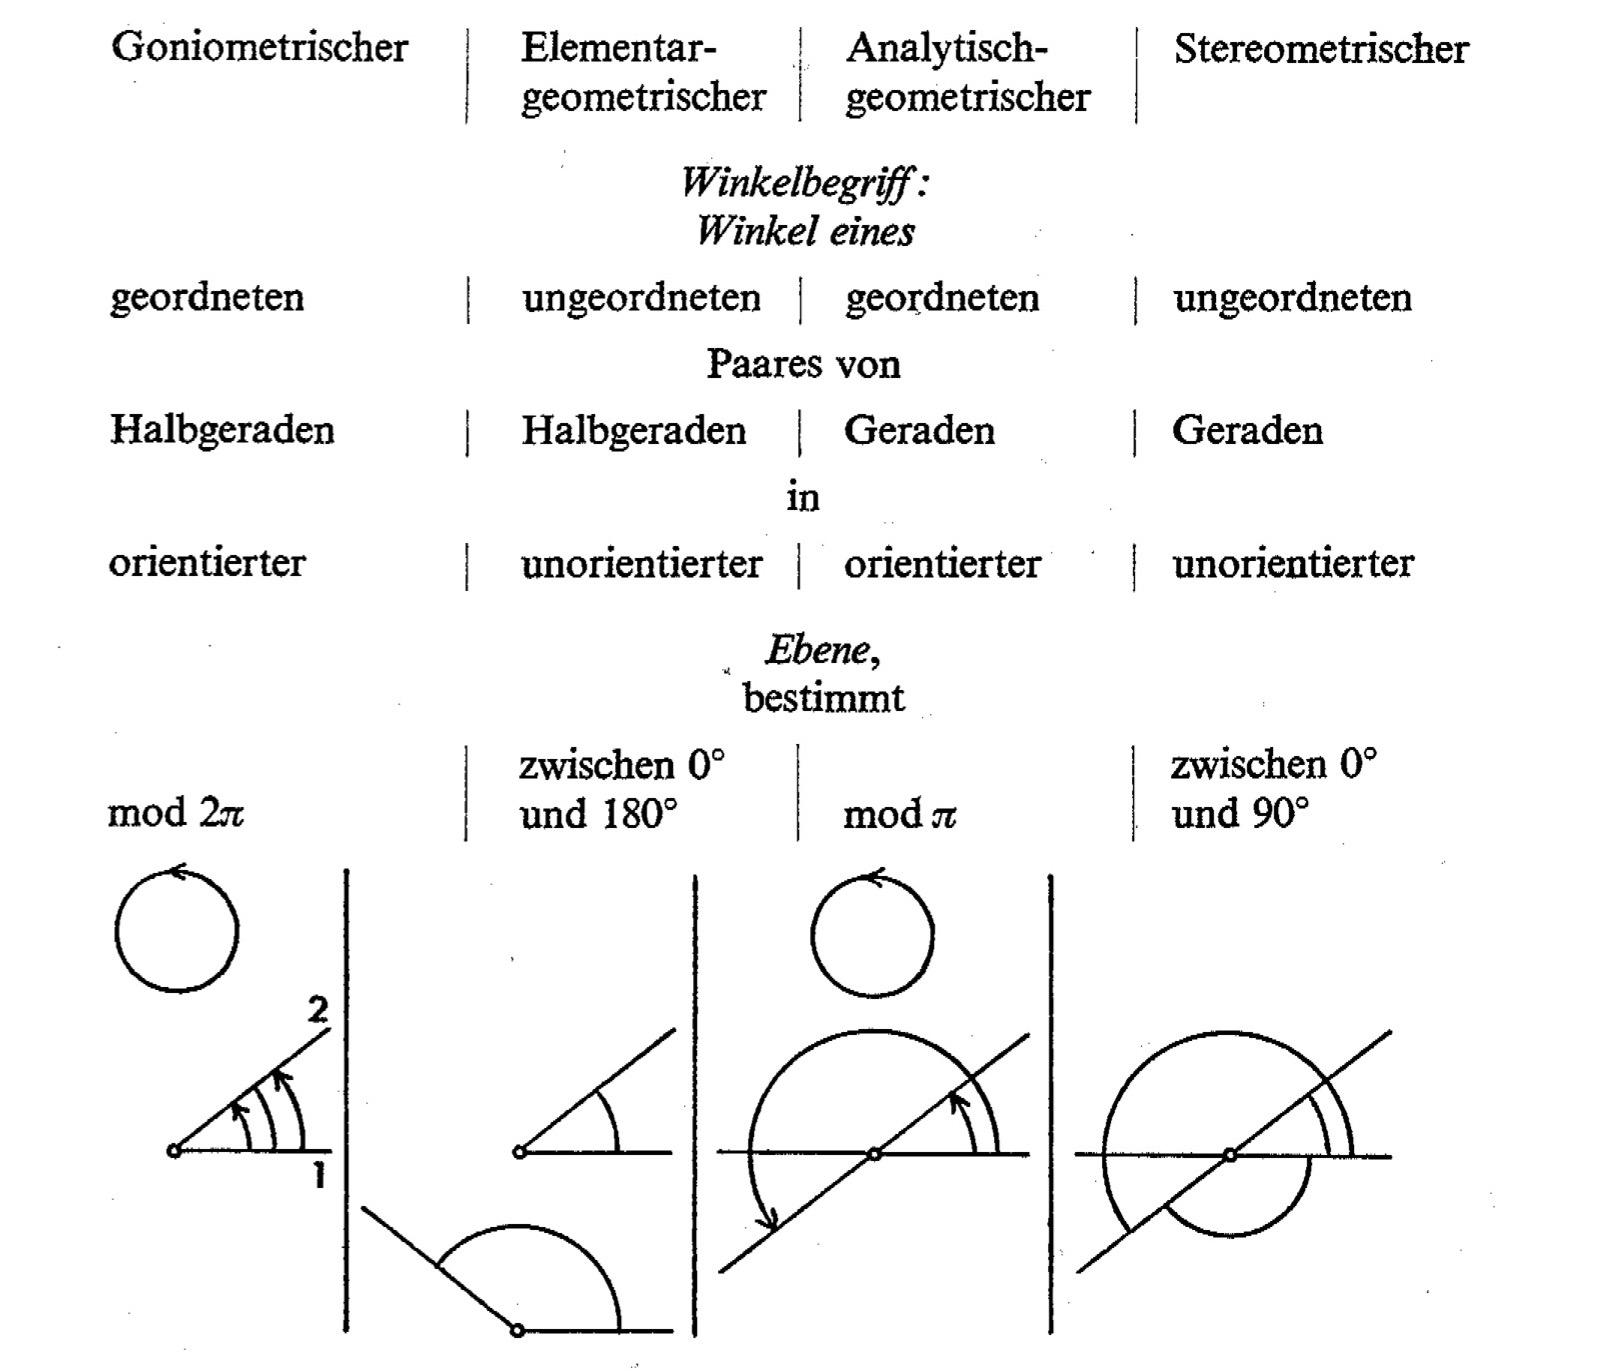
\includegraphics[width=0.75\linewidth]{pictures/2-FreudenthalWinkel} 

}

\caption{Winkelbegriffe nach \protect\hyperlink{ref-Freudenthal:1973}{Freudenthal} (\protect\hyperlink{ref-Freudenthal:1973}{1973, S. 441})}\label{fig:FreudenthalWinkel}
\end{figure}

Er diskutiert, welchen Einfluss die jeweilige Sichtweise auf dem Maßbereich hat, wie Winkel überhaupt gemessen werden können und wie mit Winkeln operiert werden kann. Was passiert denn, wenn man ein geordnetes Strahlenpaar in der orientierten Ebene spiegelt (vgl. \protect\hyperlink{ref-Freudenthal:1973}{Freudenthal, 1973, S. 443~ff.})?

Wenn die Reihenfolge der Strahlen erhalten bleibt und die Winkelmessung aufgrund der Orientierung der Ebene vorgegeben ist, ändert sich damit ggf. auch das Maß des Winkels (siehe Abbildung \ref{fig:FreudenthalWinkelSpiegeln}).



\begin{figure}

{\centering 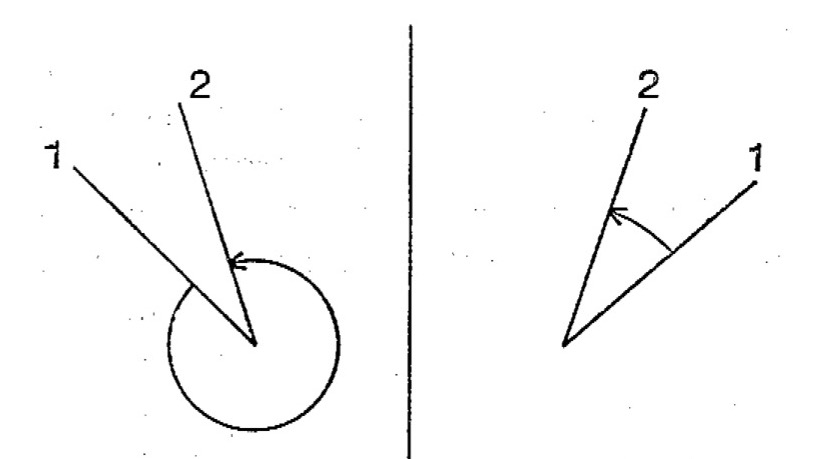
\includegraphics[width=0.5\linewidth]{pictures/2-FreudenthalWinkelSpiegeln} 

}

\caption{Spiegelung eines goniometrischen Winkels (\protect\hyperlink{ref-Freudenthal:1973}{Freudenthal, 1973, S. 443})}\label{fig:FreudenthalWinkelSpiegeln}
\end{figure}

Hierzu stellt \protect\hyperlink{ref-Freudenthal:1973}{Freudenthal} (\protect\hyperlink{ref-Freudenthal:1973}{1973, S. 443~ff.}) weitere fachmathematische Ausführungen dar und schließt damit, dass der elementargeometrische, goniometrische und analytische Winkelbegriff aus fachlicher Sicht für den schulischen Lernpfad unentbehrlich sind (\protect\hyperlink{ref-Freudenthal:1973}{Freudenthal, 1973, S. 449}).

Die \emph{Spezifizierung} besteht also darin, den Begriff zu schärfen und Operationen mit ihm zu beschreiben. Die \emph{Strukturierung} besteht u.~a. in der vernetzenden Analyse der verschiedenen Winkelbegriffe und der Schlussfolgerung ihrer gleichermaßen Bedeutsamkeit für den Schulunterricht.

\hypertarget{semantische-ebene}{%
\subsection{Semantische Ebene}\label{semantische-ebene}}

Dazu, welche Vorstellungen Schülerinnen und Schüler zum Winkelbegriff entwickeln sollen, sei u.~a. auf \protect\hyperlink{ref-Krainer:1989}{Krainer} (\protect\hyperlink{ref-Krainer:1989}{1989}) und \protect\hyperlink{ref-Mitchelmore:1998}{Mitchelmore \& White} (\protect\hyperlink{ref-Mitchelmore:1998}{1998}) verwiesen. Eine grundsätzliche Schwierigkeit beim Unterrichten von Winkeln sind diverse und nicht in Verbindung zu bringende Anwendungskontexte, die dennoch über denselben mathematischen Begriff beschrieben werden können. So ist das Sichtfeld eines Tieres ebenso wie die Umdrehung eines Wasserzählers über Winkel beschreibbar -- haben doch beide Situationen zunächst nichts miteinander zu tun.

Aufbauend auf den Arbeiten von \protect\hyperlink{ref-Krainer:1989}{Krainer} (\protect\hyperlink{ref-Krainer:1989}{1989}) und \protect\hyperlink{ref-Mitchelmore:1998}{Mitchelmore \& White} (\protect\hyperlink{ref-Mitchelmore:1998}{1998}) können über eine Verknüpfung zur formalen Ebene mithilfe einer \emph{informationstheoretischen Winkeldefinition} (\protect\hyperlink{ref-Etzold2021}{Etzold, 2021, S. 39~f..}) vier Grundvorstellungen zum Winkelbegriff ausgearbeitet bzw. validiert werden:

\begin{itemize}
\tightlist
\item
  Winkel als Knick
\item
  Winkel als Feld
\item
  Winkel als Richtungsänderung
\item
  Winkel als Umdrehung
\end{itemize}

Dabei erhalten die \emph{Bestandteile} eines Winkels (Scheitelpunkt, Schenkel, ggf. Bereich zwischen den Schenkeln, Abweichungsmaß) eine besondere Bedeutung, über die sich auch eine sinnvolle Reihenfolge der Behandlung dieser Grundvorstellungen ableiten lässt. So »bietet es sich an, mit den Winkelfeldern zu beginnen. Bei diesen werden die meisten Bestandteile sichtbar (Scheitelpunkt, beide Schenkel als Begrenzungen sowie der zwischen den Schenkeln relevante Bereich) {[}\ldots{]}. Anschließend können Knicke oder Richtungsänderungen behandelt werden, woraufhin die Umdrehungen folgen.« (\protect\hyperlink{ref-Etzold2021}{Etzold, 2021, S. 60})

Die \emph{Spezifizierung} in diesem semantischen Teil ist demnach die Ausarbeitung der Grundvorstellungen. Die Begründung einer möglichen Reihenfolge kann der \emph{Strukturierung} des Lerngegenstands zugeordnet werden.

\hypertarget{konkrete-ebene}{%
\subsection{Konkrete Ebene}\label{konkrete-ebene}}

Um die einzelnen Vorstellungen zu Winkeln aufzubauen, bedarf es charakteristischer Situationen, an denen der mathematische Kern der jeweiligen Vorstellung besonders gut sichtbar wird. Abbildung \ref{fig:Winkelsituationen} zeigt derartige \emph{Winkelsituationen} und die zugehörigen Grundvorstellungen (hier \emph{Winkelkontexte}).



\begin{figure}

{\centering 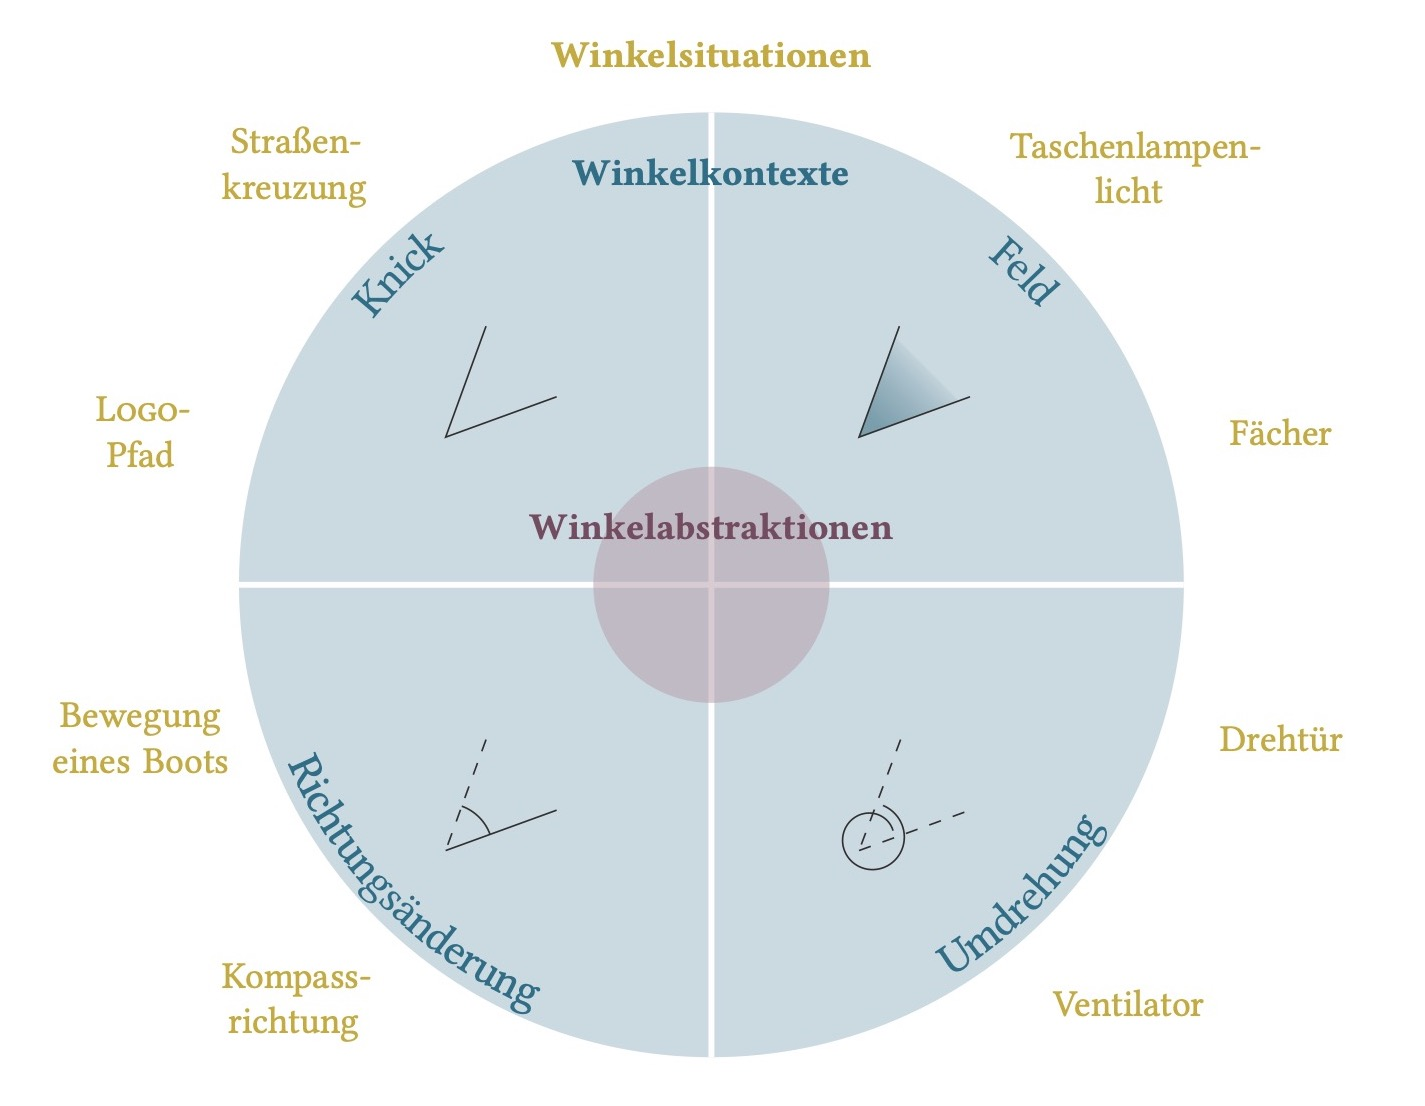
\includegraphics[width=0.75\linewidth]{pictures/2-Winkelsituationen} 

}

\caption{Winkelsituationen und -kontexte (\protect\hyperlink{ref-Etzold2021}{Etzold, 2021, S. 70})}\label{fig:Winkelsituationen}
\end{figure}

Exemplarisch für die Grundvorstellung des Winkels als Feld wird darauf aufbauend eine Lernumgebung und darin eingebettetes Unterrichtsmaterial entwickelt, mithilfe dessen die Grundvorstellung ausgebildet werden kann. An der konkreten Situation der \emph{Sichtfelder von Tieren} sollen die Schülerinnen und Schüler Handlungen ausführen, die es ihnen ermöglicht, den mathematischen Kern hinter dem konkreten Beispiel zu erkunden.

Die Schülerinnen und Schüler nutzen dazu eine App (siehe Abbildung \ref{fig:WinkelfarmApp}), in der mehrere Tiere mit ihren Sichtfeldern dargestellt werden können, und erhalten u.~a. folgende Aufgaben (vgl. \protect\hyperlink{ref-Etzold:2019Praxis4}{Etzold, 2019b, S. 8~ff.}):

\begin{enumerate}
\def\labelenumi{\arabic{enumi}.}
\tightlist
\item
  Setze das Schaf an eine Stelle, an der es von der Kuh gesehen wird, aber die Kuh selbst nicht sieht.
\item
  Setze das Schaf an eine Stelle, an der es nicht von der Kuh gesehen wird.
\item
  Das Schaf will die Kuh verwirren. Bewege es an möglichst viele Orte, an denen es von der Kuh gesehen wird.
\item
  Setze das Schaf an eine Stelle, an der es noch gerade so von der Kuh gesehen wird.
\item
  Wo muss das Schaf lang laufen, damit es die gesamte Zeit gerade so von der Kuh gesehen wird?
\end{enumerate}

An Aufgabe 5 kann z.~B. erkundet werde, dass sich das Schaf geradlinig auf der Grenze zwischen Sichtfeld und Nicht-Sichtfeld bewegen muss. In die eine Richtung ist die Bewegung beliebig fortsetzbar, in die andere durch den Kopf der Kuh begrenzt. Eine mathematische Verallgemeinerung dieser Handlung besteht dann in der Identifizierung des Schenkels (Begrenzung) als Strahl (nur in eine Richtung fortsetzbar) mit dem Scheitelpunkt (Kopf der Kuh) als \emph{Quelle} des Winkelfeldes.



\begin{figure}

{\centering 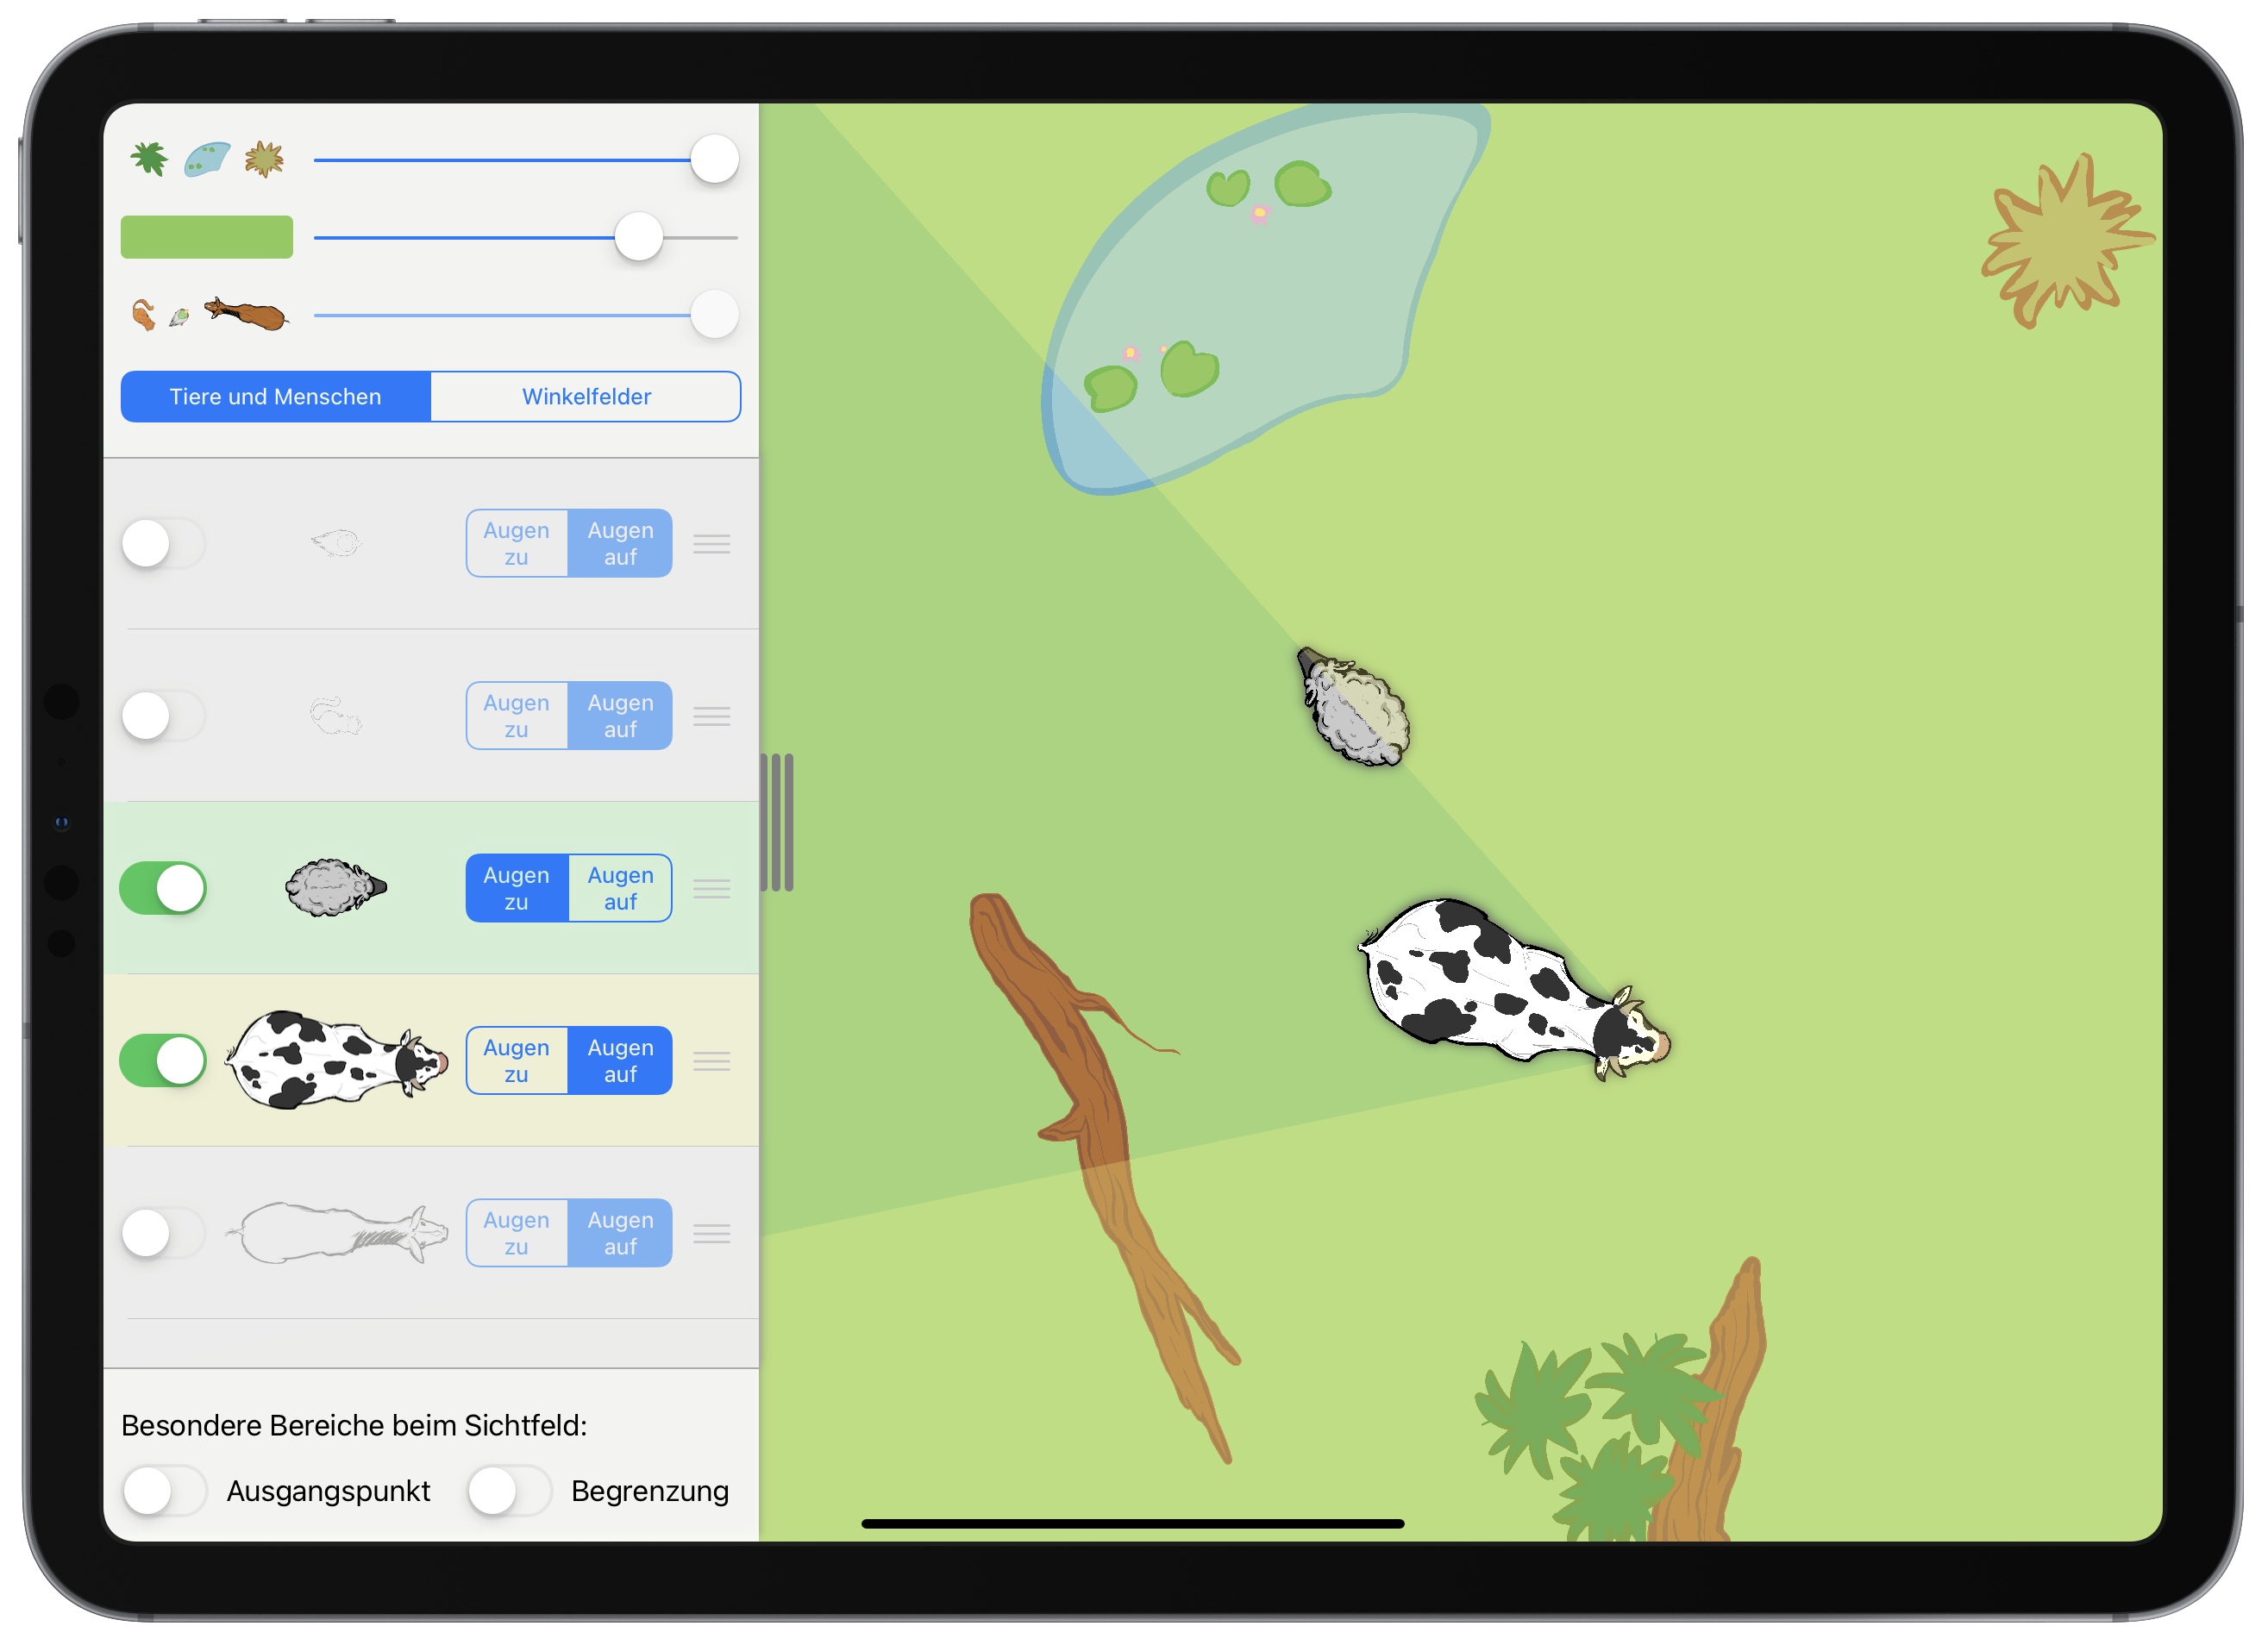
\includegraphics[width=0.75\linewidth]{pictures/2-Winkelfarm} 

}

\caption{Screenshot der App Winkel-Farm (\protect\hyperlink{ref-Etzold:2019}{Etzold, 2019a})}\label{fig:WinkelfarmApp}
\end{figure}

Als \emph{Spezifizierung} kann das Finden der Sichtfeld-Situation als charakterisches Beispiel für ein Winkelfeld angesehen werden. Die \emph{Strukturierung} führt zum dargestellten Lernpfad und den konkreten Aufgabenstellung, über die konkrete Handlungen verallgemeinert werden und damit das mathematische Verständnis aufgebaut wird.

\hypertarget{empirische-ebene}{%
\subsection{Empirische Ebene}\label{empirische-ebene}}

Die zuvor beschriebene Lernumgebung wurde in mehreren Zyklen erprobt und dabei die Qualität der Handlungen der Schülerinnen und Schüler beobachtet. Ein Ziel bestand darin, dass möglichst verallgemeinerbare Handlungen (wie oben am Beispiel des Schenkels beschrieben) durchgeführt werden.

Es wird erwartet, dass die Repräsentation eines Sichtfeldes von der Draufsicht über eine semintransparent ausgemalte Teilfläche der Ebene noch nicht bekannt ist. Um diese nachzuvollziehen und mit eigenen Erfahrungen in Bezug zu bringen, wird an den Beginn der Unterrichtsstunde ein Bild des Klassenraumes in der Draufsicht präsentiert (siehe Abbildung \ref{fig:Klassenraum}). Dann soll eine Schülerin oder ein Schüler beschreiben, was sie/er alles sieht, ohne den Kopf zu drehen. Dieser Bereich wird auf dem Bild eingezeichnet, so dass die Repräsentation des Sichtfeldes im Folgenden zur Verfügung steht.

\begin{figure}

{\centering 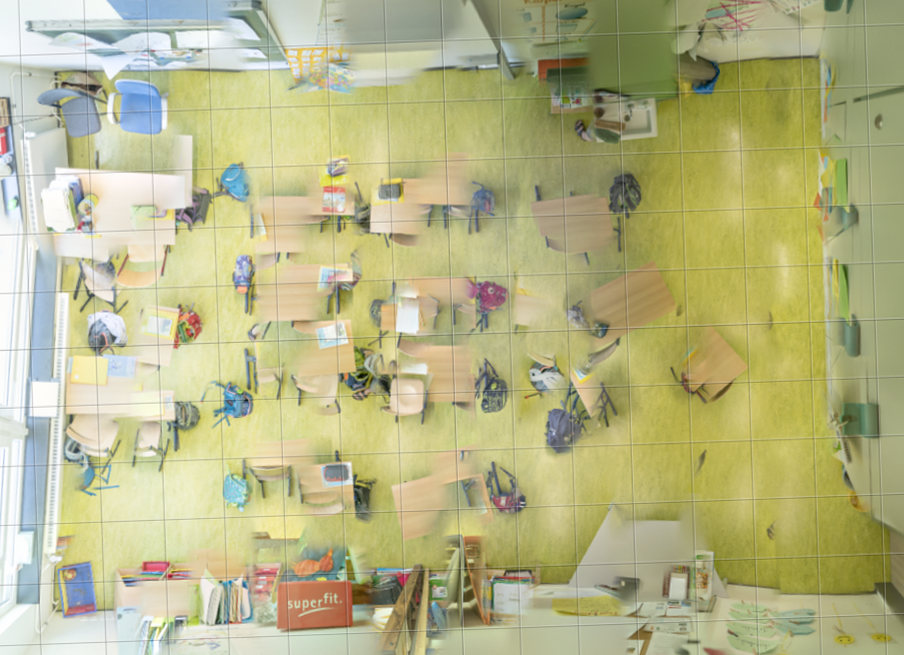
\includegraphics[width=0.75\linewidth]{pictures/2-Klassenraum} 

}

\caption{Klassenraum von oben (Foto: Christian Dohrmann)}\label{fig:Klassenraum}
\end{figure}

In der Erprobung konnte beobachtet werden, dass einige Bedienschwierigkeiten mit der Anwendung den Lernfortschritt hemmten. Dies konnte u.~a. dadurch verbessert werden, dass vor die eigentliche Erarbeitung eine freie Erkundungsphase mit der App (siehe Abbildung \ref{fig:WinkelfarmStart}) gesetzt wurde (\protect\hyperlink{ref-Etzold2021}{Etzold, 2021, S. 147, 152}). Durch spezifische Aufgabenstellungen wurden bestimmte Funktionen der App fokussiert:

\begin{figure}

{\centering 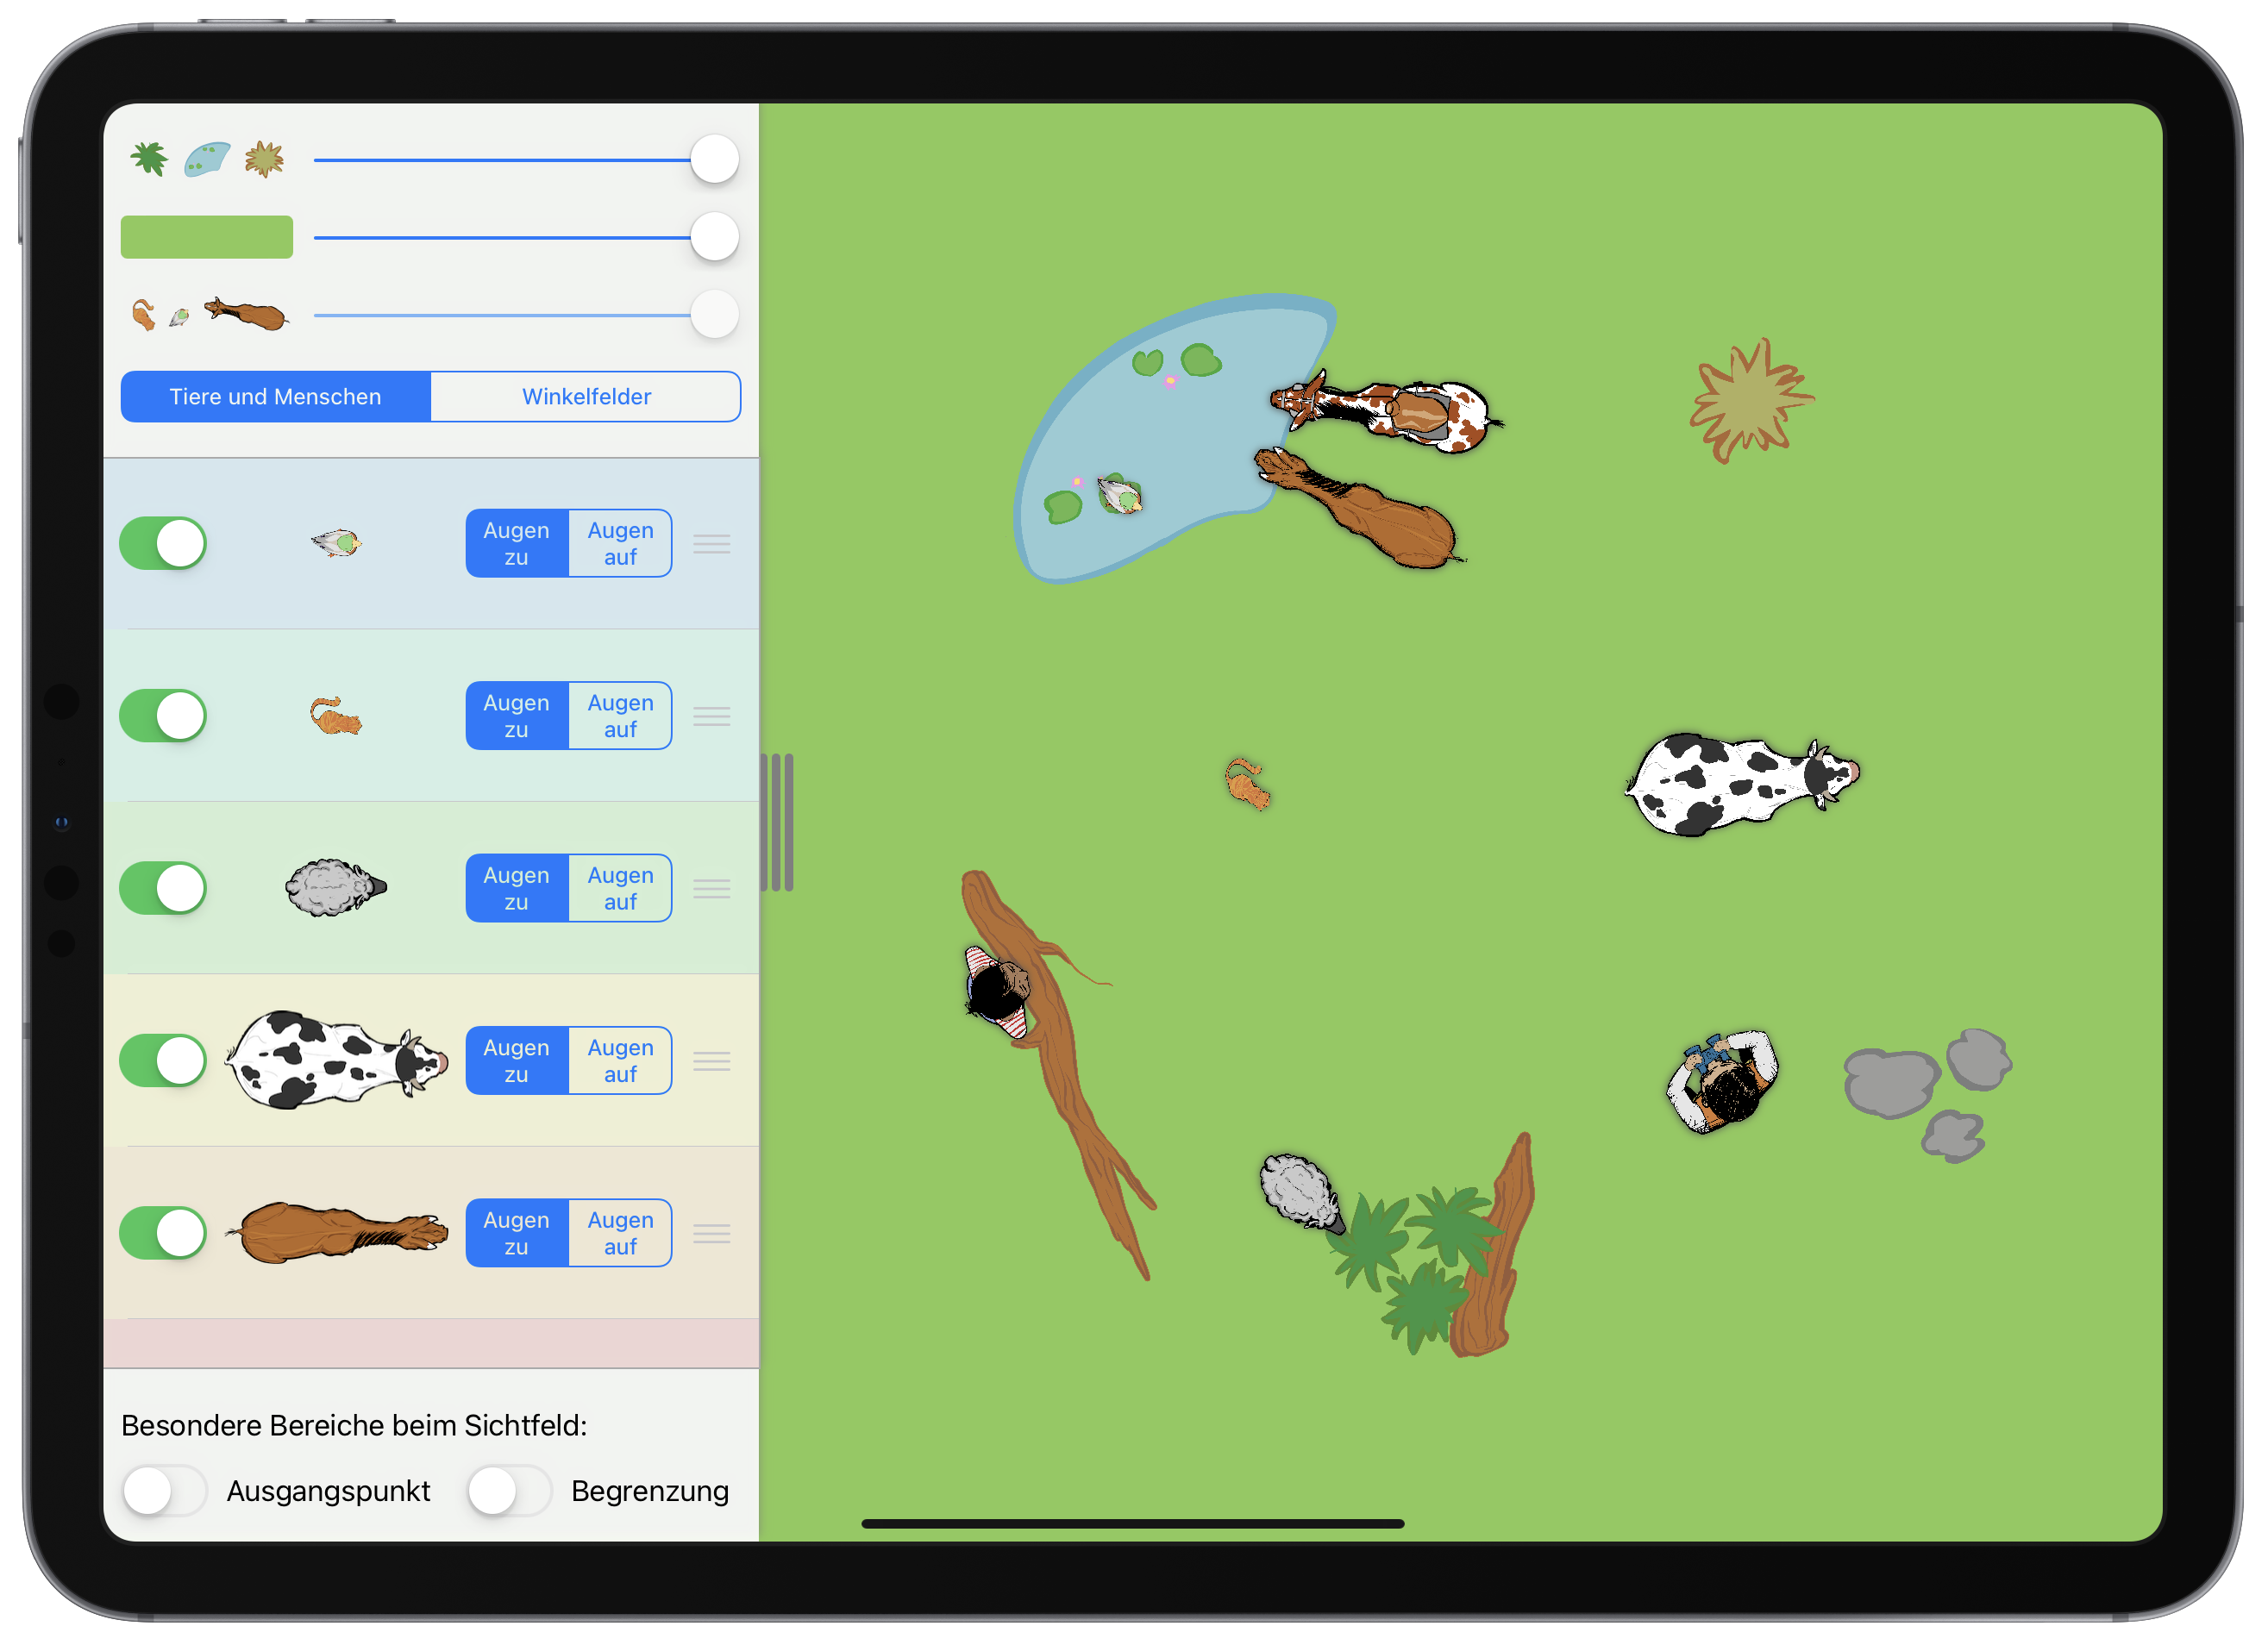
\includegraphics[width=0.75\linewidth]{pictures/2-WinkelfarmStart} 

}

\caption{Möglicher Startbildschirm für die freie Erkundungphase}\label{fig:WinkelfarmStart}
\end{figure}

\emph{»Das Pferd soll auf dem Steinpflaster stehen, die Frau soll auf dem Pferd sitzen/stehen. Das Pferd guckt in Richtung der grünen Büsche, die Frau hat die Augen zu. Gleichzeitig versteckt sich die Katze unter der Kuh.«}

Die Einführungsphase über das Klassenraumfoto folgt aus der \emph{Spezifizierung} innerhalb der empirischen Ebene. Das Hinzufügen der freien Erkundungsphase ist dagegen der \emph{Strukturierung} der Analyse zuzuordnen.

\hypertarget{verknuxfcpfung-der-ebenen}{%
\subsection{Verknüpfung der Ebenen}\label{verknuxfcpfung-der-ebenen}}

An den Ausführungen ist schon sichtbar geworden, dass sich die Ebenen nicht immer trennen lassen und teilweise gegenseitig beeinflussen. Auch gehen oft Spezifizierung und Strukturierung ineinander über.

Das ist aber gar nicht schlimm, ganz im Gegenteil. Es zeigt wieder einmal, wie wichtig solch ein ganzheitlicher Ansatz ist, so dass eine stoffdidaktische Analyse aus den diversen Sichtpunkten heraus betrachtet werden sollte.

Wichtig ist v.~a., dass Sie sich als Lehrkraft stets darüber im Klaren sind, dass für eine stoffdidaktische Analyse verschiedene Perspektiven verfolgt werden müssen. Sehen sie den Vier-Ebenen-Ansatz daher auch als Kontrollinstrument, ob Sie an alles gedacht haben, wenn Sie einen Lerngegenstand intensiv analysieren.

\hypertarget{vier-ebenen-nachbereitung}{%
\section{Zum Nachbereiten}\label{vier-ebenen-nachbereitung}}

\begin{enumerate}
\def\labelenumi{\arabic{enumi}.}
\tightlist
\item
  Lesen Sie den Artikel von \protect\hyperlink{ref-Hussmann:2016}{Hußmann \& Prediger} (\protect\hyperlink{ref-Hussmann:2016}{2016}) zum Vier-Ebenen-Ansatz.
\item
  Reflektieren Sie Ihre bisherige Fach- und Fachdidaktikausbildung in Mathematik dahingehend, welche der aufgeworfenen Fragen Sie zu konkreten Themenbereichen beantworten könnten.
\end{enumerate}

\hypertarget{part-formale-und-semantische-ebene}{%
\part*{Formale und Semantische Ebene}\label{part-formale-und-semantische-ebene}}
\addcontentsline{toc}{part}{Formale und Semantische Ebene}

\hypertarget{fundamentale-ideen}{%
\chapter{Fundamentale Ideen}\label{fundamentale-ideen}}

\begin{quote}
\textbf{Lernziele}

\begin{itemize}
\tightlist
\item
  Sie können Fundamentale Ideen über ihre Kriterien definieren.
\item
  Sie kennen Beispiele für Fundamentale Ideen, auch über die in den Bildungsstandards beschriebenen Kompetenzen hinaus.
\item
  Sie können bei einzelnen Unterrichtsinhalten den Zusammenhang zu zugehörigen Fundamentalen Ideen herstellen.
\end{itemize}

\textbf{Material}

\begin{itemize}
\tightlist
\item
  Folien zur Vorlesung zu Fundamentalen Ideen (\href{files/Stoffdidaktik-WiSe2122-Kap3.pdf}{pdf}, \href{files/Stoffdidaktik-WiSe2122-Kap3.key}{Keynote})
\end{itemize}
\end{quote}

\hypertarget{fundamentale-ideen-begriffsklaerung}{%
\section{Begriffsklärung}\label{fundamentale-ideen-begriffsklaerung}}

Die Entwicklung Fundamentaler Ideen beruft sich auf Bruners Annahme, dass »jedes Kind {[}\ldots{]} auf jeder Entwicklungsstufe jeder Lehrgegenstand in einer intellektuell ehrlichen Form erfolgreich gelehrt werden« kann (vgl. \protect\hyperlink{ref-Bruner:1976}{Bruner, 1976, S. 77}). Voraussetzung dafür ist, dass die \emph{Struktur} eines Inhaltsbereichs in einer Art und Weise präsentiert wird, dass sie dem Kind zugänglich wird. Diese \emph{hinter den Dingen} liegende Struktur hebt sich vom konkreten Inhaltsbereichen ab, ist allgemeinerer Natur und kann daher über \emph{Fundamentale Ideen} beschrieben werden.

Ziel der Orientierung des Unterrichtens an Fundamentalen Ideen besteht v.~a. darin, die (oftmals) isolierten Stoffelementen einzuordnen und in einem größeren Ganzen zu sehen. Im Umkehrschluss heißt dies aber auch, dass die Auswahl des konkreten Stoffes daran orientiert sein muss, wie dieser dazu beitragen kann, den dahinter liegenden mathematischen Kern und die zugehörigen Fundamentalen Ideen zu vertreten.

Die dazu seit den 1960er Jahren in Gang gesetzte Forschung führte zu vielfältigen Vorschlägen Fundamentaler Ideen der Mathematik -- jedoch bisher nicht zu einem allgemeingültigen Katalog. Dieser Vielfalt in den Formulierungen und Kategorisierungen kann begegnet werden, indem Fundamentale Ideen über Eigenschaften charakterisiert werden. Im Rahmen dieser Veranstaltung wird folgende Definition genutzt, zitiert aus \protect\hyperlink{ref-Schwill:1994}{Schwill} (\protect\hyperlink{ref-Schwill:1994}{1994}).

\begin{definition}[Fundamentale Idee]
\protect\hypertarget{def:FundamentaleIdee}{}\label{def:FundamentaleIdee}

Eine \textbf{Fundamentale Idee} bzgl. eines Gegenstandsbereichs (Wissenschaft, Teilgebiet) ist ein \textbf{Denk-, Handlungs-, Beschreibungs- oder Erklärungsschema}, das

\begin{enumerate}
\def\labelenumi{\arabic{enumi}.}
\tightlist
\item
  in verschiedenen Gebieten des Bereichs vielfältig anwendbar oder erkennbar ist (\textbf{Horizontalkriterium}),
\item
  auf jedem intellektuellen Niveau aufgezeigt und vermittelt werden kann (\textbf{Vertikalkriterium}),
\item
  in der historischen Entwicklung des Bereichs deutlich wahrnehmbar ist und längerfristig relevant bleibt (\textbf{Zeitkriterium}),
\item
  einen Bezug zu Sprache und Denken des Alltags und der Lebenswelt besitzt (\textbf{Sinnkriterium}).
\end{enumerate}

\end{definition}

\begin{quote}
\textbf{Überblick zur historischen Entwicklung Fundamentaler Ideen}

\begin{itemize}
\tightlist
\item
  \protect\hyperlink{ref-Bank:2016}{von der Bank} (\protect\hyperlink{ref-Bank:2016}{2016, S. 37~ff.}): \emph{Fundamentale Ideen der Mathematik: Weiterentwicklung einer Theorie zu deren unterrichtspraktischer Nutzung}
\end{itemize}
\end{quote}

\hypertarget{auswahl-fundamentaler-ideen}{%
\section{Auswahl fundamentaler Ideen}\label{auswahl-fundamentaler-ideen}}

\hypertarget{kategorisierung}{%
\subsection{Kategorisierung}\label{kategorisierung}}

Das Fehlen eines allgemeingültigen Katalogs sollte nicht davon abhalten, bestehende Auflistungen und Strukturierungen Fundamentaler Ideen zu betrachten. Angelehnt an \protect\hyperlink{ref-vonderBank:2013}{von der Bank} (\protect\hyperlink{ref-vonderBank:2013}{2013, S. 103}) und \protect\hyperlink{ref-Lambert:2012}{Lambert} (\protect\hyperlink{ref-Lambert:2012}{2012}), die unterschiedliche Kategorisierungen analysiert haben, sollen an dieser Stelle drei grobe Bereiche festgehalten werden.

\hypertarget{inhaltsideen}{%
\subsubsection{Inhaltsideen}\label{inhaltsideen}}

Inhaltsideen beziehen sich auf konkrete Inhaltsbereiche der Mathematik, die die Kriterien Fundamentaler Ideen erfüllen können. Nicht ganz zufällig spiegeln diese sich in den Leitideen der Bildungsstandards wider (\protect\hyperlink{ref-KMK:2012}{Sekretariat der Ständigen Konferenz der Kultusminister der Länder in der Bundesrepublik Deutschland, 2012}, \protect\hyperlink{ref-KMK:2004a}{2004}).

Beispiele:

\begin{itemize}
\tightlist
\item
  Zahl
\item
  Algorithmus
\item
  Maß
\item
  Raum und Form
\item
  Funktion
\item
  Zufall
\end{itemize}

\hypertarget{schnittstellenideen}{%
\subsubsection{Schnittstellenideen}\label{schnittstellenideen}}

Schnittstellenideen haben die Eigenschaft, dass durch sie die »Mathe(matik) wirkt« und »auch für andere Fächer in ihrer je spezifischen Weise relevant sind« (\protect\hyperlink{ref-Lambert:2012}{Lambert, 2012}). Damit korrelieren sie mit den prozessbezogenen Kompetenzen der Bildungsstandards.

Beispiele:

\begin{itemize}
\tightlist
\item
  Kommunizieren
\item
  Modellieren
\item
  Argumentieren
\item
  Problemlösen
\item
  Darstellen
\item
  Fragen
\end{itemize}

\hypertarget{taetigkeitsideen}{%
\subsubsection{Tätigkeitsideen}\label{taetigkeitsideen}}

Tätigkeitsideen beziehen sich insbesondere auf innermathematische Tätigkeiten, die sich über verschiedene Inhaltsbereiche hinweg zeigen. \protect\hyperlink{ref-Lambert:2012}{Lambert} (\protect\hyperlink{ref-Lambert:2012}{2012}) betont, dass es diese (über die Bildungsstandards hinaus) ebenfalls zu beachten gilt, wenn man einen reichhaltigen Mathematikunterricht bewirken möchte.

Beispiele:

\begin{itemize}
\tightlist
\item
  Approximierung
\item
  Optimierung
\item
  Linearität/Linearisierung
\item
  Symmetrie
\item
  Invarianz
\item
  Rekursion
\item
  Vernetzung
\item
  Ordnen
\item
  Strukturierung
\item
  Formalisierung
\item
  Exaktifizierung
\item
  Verallgemeinern
\item
  Idealisieren
\end{itemize}

Im Rahmen des Projektmoduls \emph{Erweitertes Fachwissen für den schulischen Kontext in Mathematik}\footnote{siehe Modulbeschreibung bei \href{https://puls.uni-potsdam.de/qisserver/rds?state=verpublish\&status=init\&vmfile=no\&moduleCall=modulansicht\&publishConfFile=modulverwaltung\&publishSubDir=up/modulbearbeiter\&\&modul.modul_id=3156\&menuid=\&topitem=Modulbeschreibung\&subitem=}{PULS}} werden Sie insbesondere Bezüge zwischen Schul- und Hochschulmathematik auf Basis Fundamentaler Ideen herstellen, wofür die Inhalts- und Tätigkeitsideen von hoher Relevanz sind.

\begin{quote}
\textbf{Diskussion Fundamentaler Ideen in den Stoffgebieten der Sekundarstufe II}

\begin{itemize}
\tightlist
\item
  Analysis: \protect\hyperlink{ref-Tietze:2000a}{Tietze et al.} (\protect\hyperlink{ref-Tietze:2000a}{2000a})
\item
  Lineare Algebra/Analytische Geometrie: \protect\hyperlink{ref-Tietze:2000}{Tietze et al.} (\protect\hyperlink{ref-Tietze:2000}{2000b})
\item
  Stochastik: \protect\hyperlink{ref-Tietze:2002}{Tietze et al.} (\protect\hyperlink{ref-Tietze:2002}{2002})
\end{itemize}
\end{quote}

\hypertarget{beispiel-linearitaet}{%
\subsection{Beispiel Linearität}\label{beispiel-linearitaet}}

\hypertarget{horizontal--und-vertikalkriterium}{%
\subsubsection{Horizontal- und Vertikalkriterium}\label{horizontal--und-vertikalkriterium}}

Linearität ist ein wesentliches Konzept über die gesamte Schullaufbahn hinweg (und darüber hinaus). Dies spiegelt sich in vielfältigen Themenbereichen wider, die sowohl die Breite (\emph{Horizontalkriterium}) als auch Tiefe (\emph{Vertikalkriterium}) von Linearität und (später) auch Linearisierung zeigen. Dieser Abschnitt orientiert sich an den Darstellungen von \protect\hyperlink{ref-Danckwerts:1988}{Danckwerts} (\protect\hyperlink{ref-Danckwerts:1988}{1988}).

\begin{itemize}
\tightlist
\item
  Linearität als Phänomen tritt schon im Geometrieunterricht der Grundschule mit \textbf{Geraden} als essentielle geometrische Objekte auf. In der euklidischen Geometrie sind Geraden neben Punkten die Basisobjekte eines axiomatischen Aufbaus.
\item
  Das \textbf{Distributivgesetz} \(a\cdot (b+c) = a\cdot b + a\cdot c\), ebenfalls bereits in der Grundschule behandelt, beschreibt einen linearen Vorgang und bietet die Grundlage für die halbschriftliche Multiplikation. Über die Schulmathematik hinaus dient es z.~B. als eines der Vektorraumaxione (Skalarmultiplikation).
\item
  Das Bestimmen eines \textbf{Rechteckflächeninhalts} ist ein linearer Vorgang: Ein Rechteck, das doppelt so breit ist, hat (bei gleicher Höhe) einen doppelt so großen Flächeninhalt. Betrachtet man diese Eigenschaft nicht als Phänomen, sondern als Forderung an eine Flächeninhaltsformel, so kann aus den Bedingungen \(A(a_1+a_2,b) = A(a_1,b) + A(a_2,b)\) und \(A(a,b_1+b_2) = A(a,b_1)+A(a,b_2)\) sowie der Stetigkeit in \(\mathbb{R}^+\) die Formel \(A(a,b) = a\cdot b\) abgeleitet werden.
\item
  Lineare Zuordnungen der Art \(f(x+y) = f(x)+f(y)\) werden zu Beginn der Sekundarstufe I als \textbf{proportionale Zuordnungen} behandelt. Dies wird fortgeführt bei \textbf{linearen Funktionen} der Art \(f(x) = mx+n\), in der Fachmathematik als affin-lineare Abbildungen bezeichnet.
\item
  \textbf{Lineare Gleichungen und Gleichungssysteme} sind ebenfalls bedeutsamer Bestandteil des Mathematikunterrichts. Überhaupt baut die gesamte \textbf{Lineare Algebra} auf lineare und affin-lineare Abbildungen auf.
\item
  Die \textbf{Strahlensätze} beschreiben ebenfalls ein lineares Verhalten: Geradenabschnitte in \(c\)-facher Entfernung sind \(c\) mal so lang.
\end{itemize}

\begin{figure}

{\centering 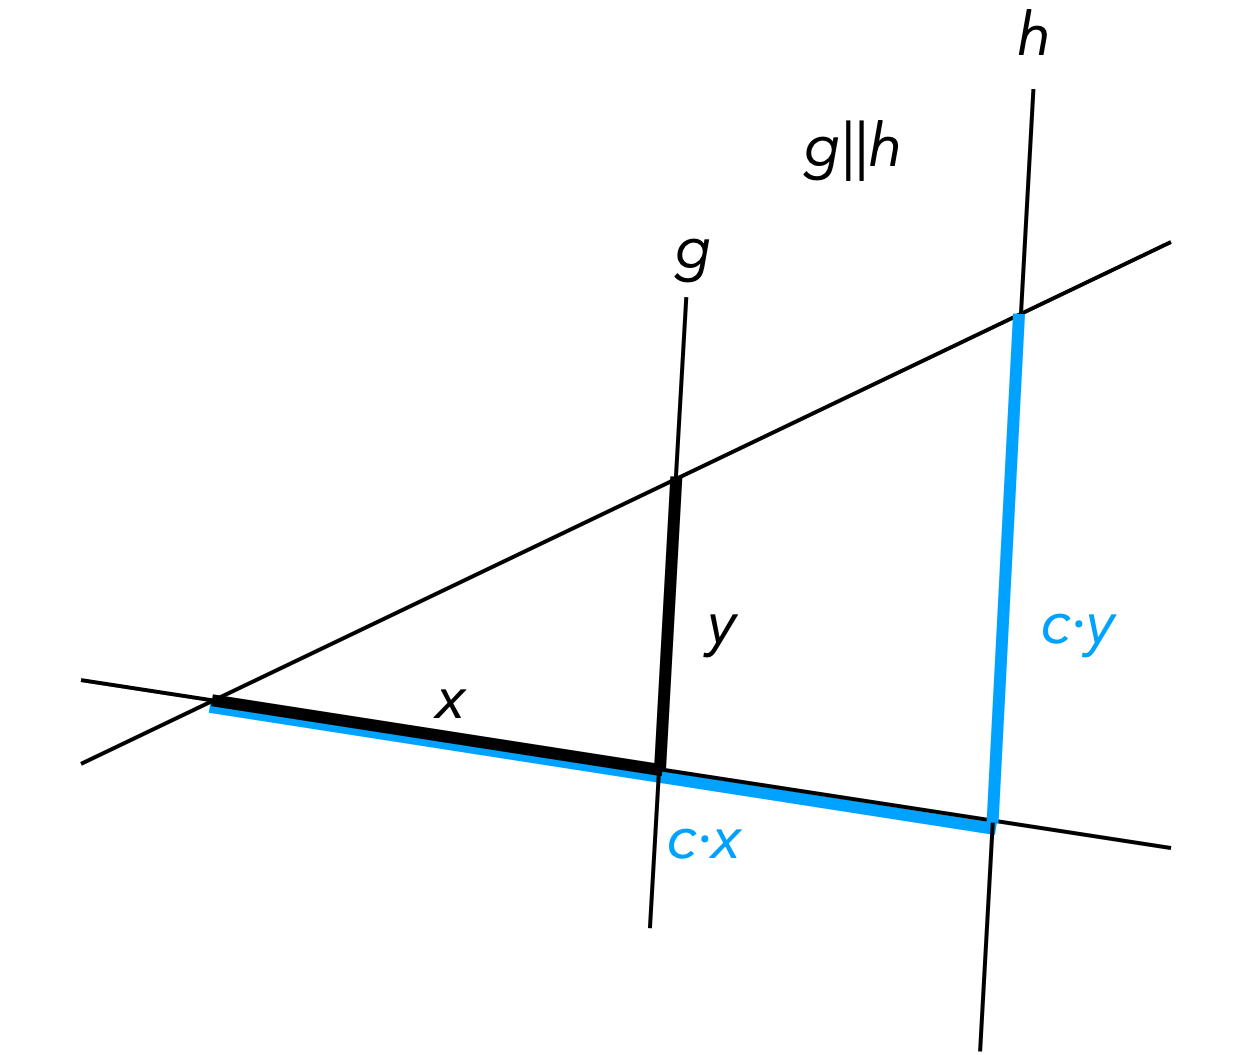
\includegraphics[width=0.5\linewidth]{pictures/3-Strahlensatz} 

}

\caption{Strahlensatzfigur}\label{fig:Strahlensatz}
\end{figure}

\begin{itemize}
\tightlist
\item
  Beim \textbf{Ableitungsbegriff} ist eine wesentliche Vorstellung, dass die Funktion in der Umgebung der zu betrachtenden Stelle linearisiert wird. Insbesondere bei höherdimensionalen Funktionen wird der Linearisierungsansatz weiterverfolgt. Die ebenfalls vorherrschende Tangentenvorstellung ist auf beliebige Dimensionen nicht übertragbar -- der Linearisierungsansatz aufgrund seiner algebraischen Beschreibung schon.\\
\item
  Eng an den Linearisierungsansatz angelehnt ist die \textbf{lineare Approximation} von Funktionen (z.~B. \(sin(x)\approx x\) für \(x\approx 0\)). Die führt sich in der Hochschulmathematik fort, beispielsweise bei Taylor-Reihen.\\
\item
  Das Bedürfnis der Linearisierung, insbesondere aus der Physik heraus, zeigt sich auch bei der Nutzung \textbf{spezifisch skalierter Diagrammachsen}, z.~B. von Logarithmuspapier. Wegen der Äquivalenz von \(y = c\cdot a^x\) und \(\ln y = (\ln a )\cdot x + \ln c\) lassen sich beliebige Exponentialfunktionen auf Logarithmuspapier als lineare Funktionen darstellen.
\item
  Verschiedene Näherungsverfahren, wie das \textbf{Newton-Verfahren}, bedienen ebenfalls sich der Linearisierung.
\end{itemize}

An dieser Stelle sei darauf hingewiesen, dass Linearität derart fundamental ist, dass selbst nicht-lineare Zusammenhänge häufig fälschlicherweise als linear angenommen werden. Dies zeigt sich zum Beispiel an den Fehlannahmen \((x+y)^2 \overset{?!}{=} x^2+y^2\), \(\sqrt{x+y} \overset{?!}{=} \sqrt{x}+\sqrt{y}\) oder \(\sin(x+y) \overset{?!}{=} \sin(x)+\sin(y)\). Derartige Fehler können Sie als Lehrkraft besser einordnen (und korrigieren), wenn Sie sich der Fundamentalen Idee \emph{Linearität} (die hier eben \emph{nicht} gilt) bewusst sind. Insbesondere spricht dies auch für ein Explizitmachen der Fundamentalen Idee Ihren Schülerinnen und Schülern gegenüber, so dass Sie derartigen Fehlern nicht nur mit Gegenbeispielen entgegen treten können, sondern auch eine strukturelle Einordnung sichtbar machen können.

Gerade wegen der genannten Fehlannahmen und der für die Schülerinnen und Schüler i.~d.~R. nicht in Zusammenhang gebrachten Dualität aus \emph{geradlinig} und \emph{additiv und homogen} sehen \protect\hyperlink{ref-Tietze:2002}{Tietze et al.} (\protect\hyperlink{ref-Tietze:2002}{2002, S. 39}) die Linearität dagegen nicht als eine im Mathematikunterricht etablierte Fundamentale Idee, »die die Schüler erkennen und die ihr Denken ordnet und anregt«.

\hypertarget{zeit--und-sinnkriterium}{%
\subsubsection{Zeit- und Sinnkriterium}\label{zeit--und-sinnkriterium}}

Linearität zeigt sich auch in der historischen Entwicklung der Mathematik als eine prägende Leitlinie, womit sie das \emph{Zeitkriterium} Fundamentaler Ideen erfüllt. In der Linearen Algebra sei beispielsweise das Lösen linearer Gleichungssysteme im 18. Jahrhundert bis hin zum Gauß-Algorithmus im 19. Jahrhundert oder die Darstellung linearer Vorgänge mit Matrizen im 17./18. Jahrhundert erwähnt (vgl. \protect\hyperlink{ref-Tietze:2000}{Tietze et al., 2000b, S. 73~ff.}). In der Analysis spiegelt sich die Linearität bzw. Linearisierung in der gesamten Differenzialrechnung wider, von der Interpolation nach der Jahrtausendwende über Taylors \emph{Linear perspective} von 1715 (vgl. \protect\hyperlink{ref-Bruckler:2018}{Brückler, 2018, S. 39, 119}) bis in die Gegenwart der linearen Modellierung nichtlinearer Zusammenhänge.

\begin{quote}
\textbf{Historische Originalausgabe}

\protect\hyperlink{ref-Taylor:1715}{Taylor} (\protect\hyperlink{ref-Taylor:1715}{1715}): \emph{Linear perspective}
\end{quote}

Auch Alltagssituationen bzw. die Alltagssprache ist von Linearität geprägt. Beispielsweise treten proportionale Zuordnungen unmittelbar beim Einkaufen auf, wenn Waren abgewogen und der Preis bestimmt wird. Auch reale Messvorgänge, wie z.~B. die Geschwindigkeitsmessung, beziehen sich in der Regel auf die Messung von (sehr kurzen) Zeitintervallen, in denen ein lineares Verhalten angenommen wird. Das \emph{Sinnkriterium} zeigt sich aber auch in Begriffen wie \emph{lineares Fernsehen} oder \emph{lineare Erzählungen}. Dies ist zwar keine mathematische Linearität im Sinne der Formel \(f(x+y) = f(x) +f(y)\), aber der Begriff findet in einer verwandten Bedeutung in der Alltagssprache Verwendung.

\hypertarget{gegenbeispiele}{%
\subsection{Gegenbeispiele}\label{gegenbeispiele}}

Zur Verständnisförderung sollen noch ein paar Gegenbeispiele für Fundamentale Ideen angebracht werden.

\begin{itemize}
\tightlist
\item
  Das bereits erwähnte \textbf{Distributivgesetz} an sich ist zwar elementar, aber ihm fehlt die Weite, womit es nicht das Horizontalkriterium erfüllt. Die \emph{Linearität} als dahinterliegende Idee ist dagegen weit genug (vgl. ähnliche Argumentation zum \textbf{Kommutativgesetz} und der dahinterliegenden Idee der \emph{Invarianz} bei \protect\hyperlink{ref-Schubert:2011}{Schubert \& Schwill, 2011, S. 63}).
\item
  Der \textbf{Umkehrfunktion} fehlt das Sinnkriterium, da dieser Begriff in der Lebenswelt außerhab der Mathematik kaum von Relevanz ist. Dahinter liegt vielmehr die Idee der \emph{Reversibilität} als »Umkehrbarkeit von Operationen mit Wiederherstellung des Ausgangszustandes« (\protect\hyperlink{ref-Schubert:2011}{Schubert \& Schwill, 2011, S. 63}).
\end{itemize}

\hypertarget{fund.-ideen-und-stoffdidaktik}{%
\section{Fund. Ideen und Stoffdidaktik}\label{fund.-ideen-und-stoffdidaktik}}

Fundamentale Ideen haben zwar ihren Ursprung in der Fachstruktur, aber sie »sind nicht Elemente der Wissenschaft an sich, sondern Produkte unseres Verstandes, die wir der Wissenschaft aufprägen. Folglich können sie nur relativ zum Menschen objektiviert werden« (\protect\hyperlink{ref-Schubert:2011}{Schubert \& Schwill, 2011, S. 62}). Hinsichtlich des \protect\hyperlink{tab:fragen-ebenen}{Vier-Ebenen-Ansatzes} liegen sie auf der \textcolor{semanticColor}{semantischen Ebene} mit starken Bezügen zur \textcolor{formalColor}{formalen Ebene}.

Für Ihre stoffdidaktische Analyse können Fundamentale Ideen insbesondere hilfreich für die \textbf{Dekonstruktion} des Fachwissens und anschließende \textbf{Rekonstruktion} des Schulwissens sein.

Wenn sie also beispielsweise eine stoffdidaktische Analyse zur Flächeninhaltsberechnung durchführen, setzen Sie sich mit der Fundamentalen Idee des \emph{Messens} auseinander. Dabei verstehen Sie Messvorgänge als Vergleiche zu einem Standardmaß (z.~B. Kästchen auszählen), erkennen Zerlegungs- und Ergänzungsgleichheit als notwendige Prinzipien zur präziseren Beschreibung, sehen Dreiecke als bedeutsame Basisfiguren für Flächeninhaltsberechnungen an und haben den Blick für die Integralrechnung als verallgemeinerbare Methode zur Flächeninhaltsbestimmung krummliniger Figuren (vgl. \protect\hyperlink{ref-Vohns:2000}{Vohns, 2000, S. 98~ff.}). Sie \emph{dekonstruieren} (zerlegen) damit Ihr eigenes mathematisches Fachwissen.

Nun sind Sie in der Lage, das Wissen zur Flächeninhaltsberechnung für Schülerinnen und Schüler neu aufzubauen, also zu \emph{rekonstruieren} und (unter Hinzunahme der Betrachtung von Grundvorstellungen und den restlichen Ebenen des Vier-Ebenen-Ansatzes) einen Lernpfad zu entwickeln. Im Zusammenhang mit der Integralrechnung kann dies z.~B. heißen, dass Sie parallel zum Bilden von Ober- und Untersummen noch einmal eine krummlinig begrenzte Fläche durch Kästchen auszählen lassen -- ggf. mit unterschiedlicher Feinheit und einer Abschätzung nach oben und nach unten. Die Fundamentalen Ideen haben für Sie damit auch eine \emph{ordnende Funktion} des Unterrichtsstoffes.

\begin{figure}

{\centering 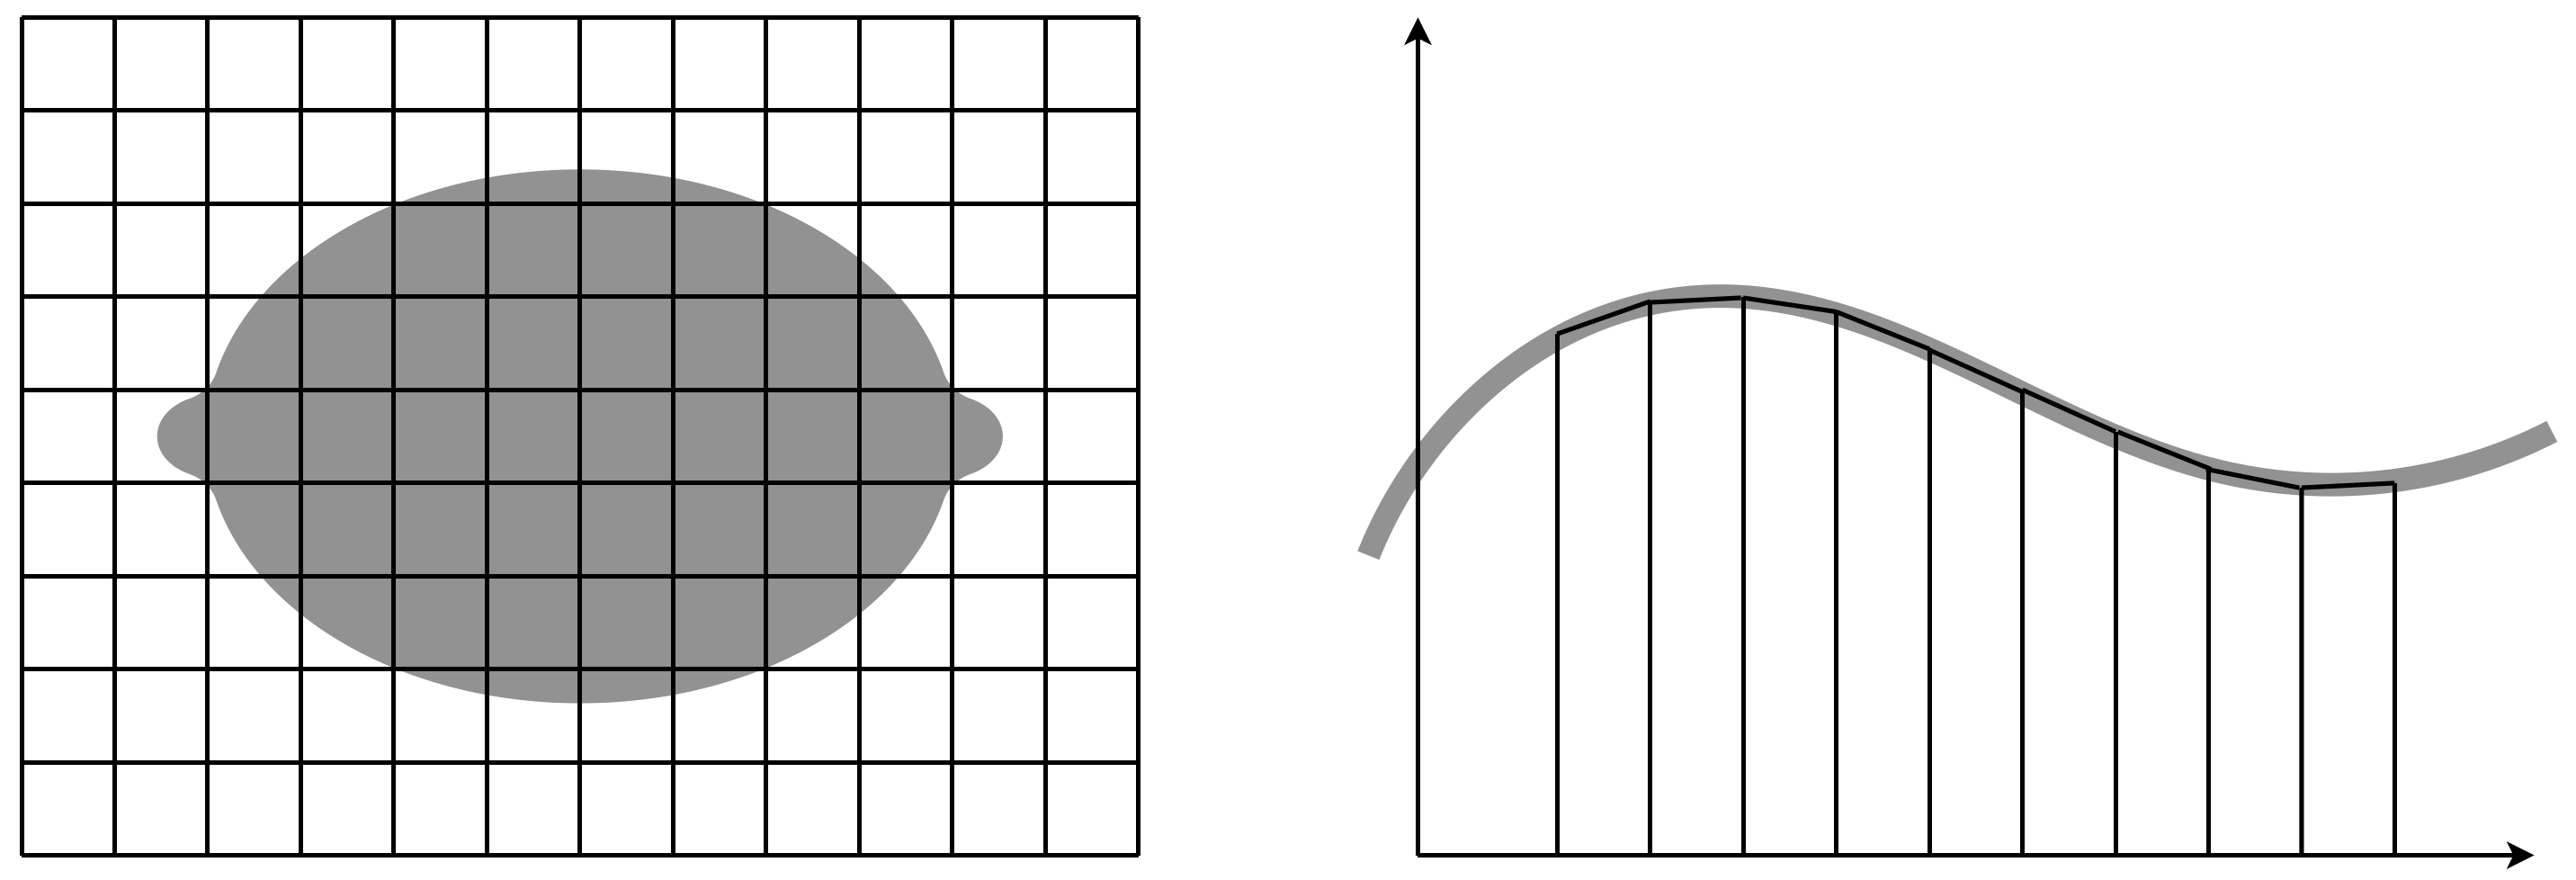
\includegraphics[width=0.75\linewidth]{pictures/3-Flaeche} 

}

\caption{Flächeninhaltsbestimmung}\label{fig:Flaeche}
\end{figure}

\hypertarget{fundamentale-ideen-nachbereitung}{%
\section{Zum Nachbereiten}\label{fundamentale-ideen-nachbereitung}}

\begin{enumerate}
\def\labelenumi{\arabic{enumi}.}
\tightlist
\item
  Lesen Sie das Kapitel 3.2.2 \emph{Der Begriff der Fundamentalen Ideen in der Pädagogik} bei \protect\hyperlink{ref-Schubert:2011}{Schubert \& Schwill} (\protect\hyperlink{ref-Schubert:2011}{2011, S. 59--65}).
\item
  Wählen Sie ein Unterrichtsthema aus und stellen Sie den Bezug zu Fundamentalen Ideen her, indem Sie die \protect\hyperlink{tab:fragen-ebenen}{zugehörigen Fragen der semantischen Ebene} beantworten.
\end{enumerate}

\hypertarget{grundvorstellungen}{%
\chapter{Grundvorstellungen}\label{grundvorstellungen}}

\begin{quote}
\textbf{Lernziele}

\begin{itemize}
\tightlist
\item
  Sie können die Grundvorstellungsidee beschreiben und wissen über deren Bedeutung für den Mathematikunterricht.
\item
  Sie kennen Grundvorstellungen zu einzelnen mathematischen Begriffen.
\end{itemize}

\textbf{Material}

\begin{itemize}
\tightlist
\item
  Folien zur Vorlesung zu Grundvorstellungen (\href{files/Stoffdidaktik-WiSe2122-Kap4.pdf}{pdf}, \href{files/Stoffdidaktik-WiSe2122-Kap4.key}{Keynote})
\end{itemize}
\end{quote}

\hypertarget{grundvorstellungen-begriffsklaerung}{%
\section{Begriffsklärung}\label{grundvorstellungen-begriffsklaerung}}

\hypertarget{grundvorstellungsidee}{%
\subsection{Grundvorstellungsidee}\label{grundvorstellungsidee}}

Als Sie zu Beginn Ihres Mathematikstudiums die Peano-Axiome zur Definition der Natürlichen Zahlen \(\mathbb{N}\) kennengelernt haben, konnten Sie dies wahrscheinlich -- trotz der Neuigkeit der formalen Beschreibung -- derart mit Ihrer Lebenswelterfahrung in Verbindung bringen, dass Natürliche Zahlen abgezählt werden können, also damit z.~B. die Platzierungen eines Wettrennens durchnummeriert werden können.

\begin{quote}
\textbf{Peano-Axiome} (\protect\hyperlink{ref-WikiPeano}{Wikipedia, 2021b})

\begin{enumerate}
\def\labelenumi{\arabic{enumi}.}
\tightlist
\item
  \(0\) ist eine natürliche Zahl.
\item
  Jede natürliche Zahl \(n\) hat eine natürliche Zahl \(n'\) als Nachfolger.
\item
  \(0\) ist kein Nachfolger einer natürlichen Zahl.
\item
  Natürliche Zahlen mit gleichem Nachfolger sind gleich.
\item
  Enthält die Menge \(X\) die \(0\) und mit jeder natürlichen Zahl \(n\) auch deren Nachfolger \(n'\), so bilden die natürlichen Zahlen eine Teilmenge von \(X\).
\end{enumerate}
\end{quote}

Dieser \textbf{Bezug auf eine bekannte Handlung} ist wesentlich dafür, dass die Definition und damit der Begriff der Natürlichen Zahlen für Sie mit einem Sinn behaftet ist. Innerhalb dieser \emph{ordinalen Sichtweise} Natürlicher Zahlen helfen nun geeignete\footnote{\emph{Geeignet} heißt in diesem Fall, dass sich die Kernaussage des Begriffs in der Repräsentation wiederfindet. Im Ordinalzahlaspekt ist dies v.~a. die Reihung von Zahlen. Was dabei (noch) nicht relevant ist, ist zum Beispiel die exakte Messbarkeit, wie man sie etwa auf dem Zahlenstrahl repräsentiert.} \textbf{Repräsentationen} dabei, sich Rechenoperationen vorstellen und sie \textbf{operativ}\footnote{\emph{Operativ} heißt hier zum Beispiel, dass Sie zu einer Aufgabe wie \(2+7\) Nachbaraufgaben (\(2+8\)), Umkehraufgaben (\(9-2\)), Platzhalteraufgaben (\(2+\boxed{\phantom{7}}=9\)) usw. aufstellen und lösen können.} auszuführen zu können, also bspw. das Addieren als ein Weiterzählen aufzufassen (siehe Abbildung \ref{fig:Addition}).

\begin{figure}

{\centering 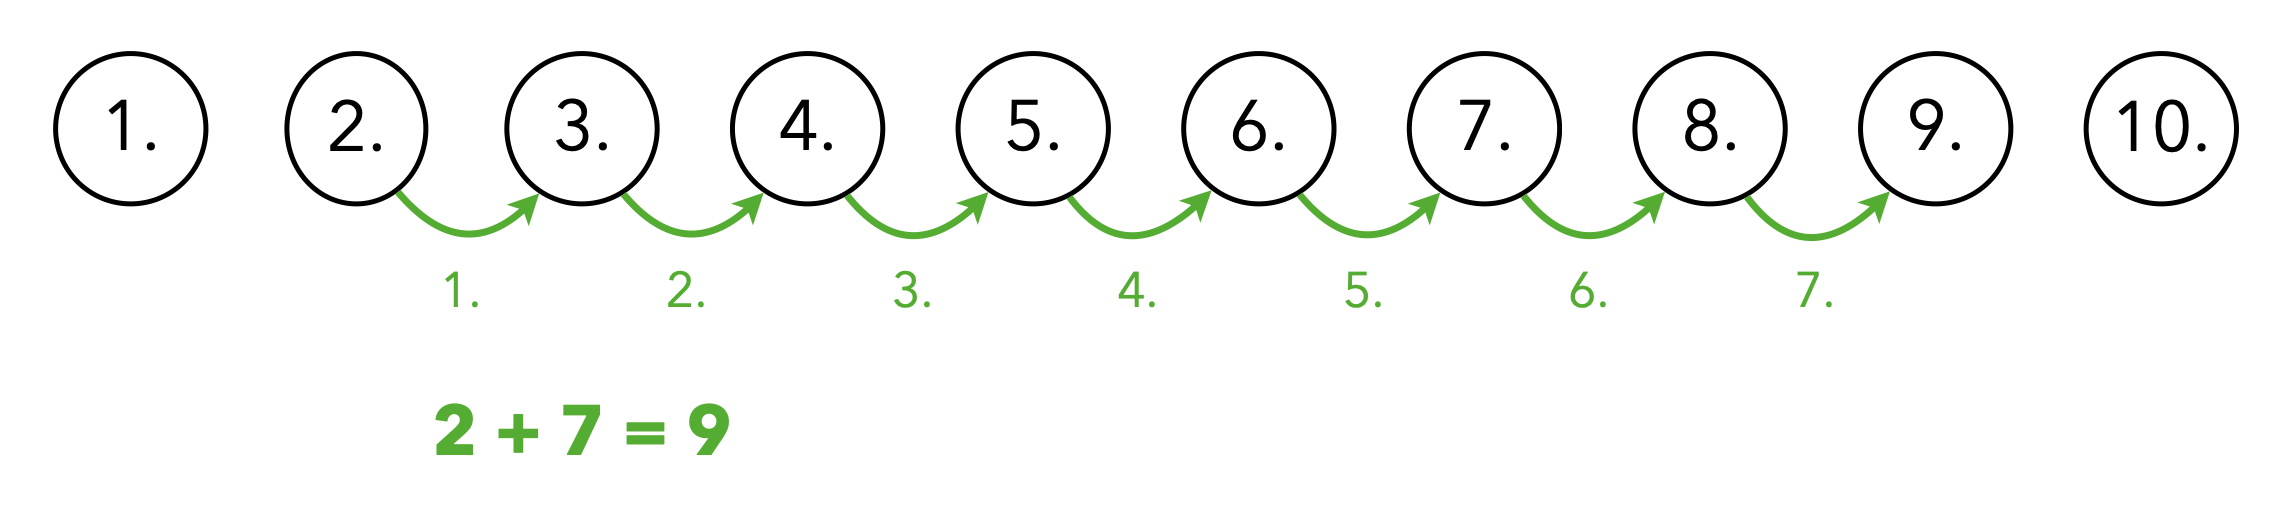
\includegraphics[width=0.75\linewidth]{pictures/4-Addition} 

}

\caption{Additionsaufgabe im ordinalen Zahlaspekt}\label{fig:Addition}
\end{figure}

Mit der Fähigkeit der Verknüpfung des mathematischen Begriffs und der Lebenswelt ist also eine \textbf{Anwendung des Begriffs auf die Wirklichkeit} möglich, insbesondere in Modellierungsprozessen. Dabei sind beide Richtungen relevant: Von der Realsituation zur Mathematik und von der Mathematik zur Realität.

Ziel des Mathematikunterrichts sollte es nun sein, für alle Begriffe ein derartiges Verständnis aufzubauen, was auch heißt, verschiedene Vorstellungen zu einem Begriff zu vermitteln. Nach \protect\hyperlink{ref-Hofe:1995}{vom Hofe} (\protect\hyperlink{ref-Hofe:1995}{1995, S. 97~f.}, Hervorhebung durch H.E.) ergibt sich daraus eine Orientierung an Grundvorstellungen im Mathematikunterricht:

\begin{definition}[Grundvorstellungen]
\protect\hypertarget{def:Grundvorstellungen}{}\label{def:Grundvorstellungen}

Die \textbf{Grundvorstellungsidee} beschreibt \textbf{Beziehungen zwischen mathematischen Inhalten und} dem Phänomen der \textbf{individuellen Begriffsbildung}. In ihren unterschiedlichen Ausprägungen charakterisiert sie mit jeweils unterschiedlichen Schwerpunkten insbesondere drei Aspekte dieses Phänomens:

\begin{itemize}
\tightlist
\item
  Sinnkonstituierung eines Begriffs durch \textbf{Anknüpfung an} bekannte \textbf{Sach- oder Handlungszusammenhänge} bzw. \textbf{Handlungsvorstellungen},\\
\item
  Aufbau entsprechender (visueller) \textbf{Repräsentationen bzw. »Verinnerlichungen«}, die \textbf{operatives Handeln} auf der Vorstellungsebene ermöglichen,\\
\item
  Fähigkeit zur Anwendung eines Begriffs auf die Wirklichkeit durch \textbf{Erkennen der} entsprechenden \textbf{Struktur in Sachzusammenhängen} oder durch \textbf{Modellieren} des Sachproblems \textbf{mit Hilfe der mathematischen Struktur}.
\end{itemize}

\end{definition}

\hypertarget{ausdifferenzierung}{%
\subsection{Ausdifferenzierung}\label{ausdifferenzierung}}

\protect\hyperlink{ref-vomHofe2014}{vom Hofe} (\protect\hyperlink{ref-vomHofe2014}{2014}) unterscheidet weiterhin zwischen \textbf{primären} und \textbf{sekundären} Grundvorstellungen, abhängig von der Erfahrungswelt der Handlungen. Während sich primäre Grundvorstellungen auf reale Handlungserfahrungen stützen (z.~B. mit Steckwürfeln in der Arithmetik), entstammen sekundäre Grundvorstellungen aus den Handlungen mit bereits im Mathematikunterricht aufgebauten Repräsentationen (z.~B. Operationen auf dem Zahlenstrahl).

Ich als Autor dieses Dokuments vertrete die Ansicht, dass Grundvorstellungen zu \textbf{Aspekten} eines Begriffs und zu \textbf{Operationen} mit diesen Begriffsaspekten formuliert werden können. So wäre das oben angebrachte Beispiel der ordinalen Anordnung der Natürlichen Zahlen ein \emph{Begriffsaspekt} mit der damit verbunden Grundvorstellung, dass die Natürlichen Zahlen eine feste Reihenfolge darstellen, beginnend bei \(0\). Das \emph{Addieren} ist eine Operation in diesem Aspekt, verbunden mit der Grundvorstellung des Weiterzählens. Eine ähnliche Unterscheidung, jedoch mit inhaltlich anderer Ausrichtung, nehmen auch \protect\hyperlink{ref-Greefrath2016}{Greefrath et al.} (\protect\hyperlink{ref-Greefrath2016}{2016, S. 17}) vor. Eine Diskussion dazu findet sich bei \protect\hyperlink{ref-Etzold2021}{Etzold} (\protect\hyperlink{ref-Etzold2021}{2021, S. 72~f.}). Die genannten Begriffs\emph{aspekte} sind jedoch nicht mit den \emph{Aspekten} der Grundvorstellungsidee in Definition \ref{def:Grundvorstellungen} zu verwechseln.
Auch wenn Sie nicht unmittelbar und sofort jeweils alle Aspekte eine Begriffs im Unterricht ansprechen werden, hilft Ihnen das Wissen über den Aspektreichtum in der Unterrichtsplanung für die Ausbildung eines umfassenden Begriffsverständnisses.

Die in Definition \ref{def:Grundvorstellungen} dargestellte Grundvorstellungsidee hat einen \textbf{normativen} Charakter, d.~h. es wird davon ausgegangen, dass (aus professioneller Sicht der Mathematikdidaktik) zu mathematischen Begriffen bestimmte Grundvorstellungen identifiziert werden können, die es im Unterricht zu vermitteln gilt. Oder anders gefragt: »Welche Grundvorstellungen sind zur Lösung des Problems aus der Sicht des Lehrenden adäquat?« (\protect\hyperlink{ref-Hofe:1995}{vom Hofe, 1995, S. 106}) Diese Sichtweise wird durch eine \textbf{deskriptive} Perspektive ergänzt: »Welche individuellen Vorstellungen lassen sich im Lösungsversuch des Schülers erkennen?« (\protect\hyperlink{ref-Hofe:1995}{vom Hofe, 1995, S. 107}) Diese über empirische Untersuchungen zu ermittelnden Vorstellungen sind das, was sich Schülerinnen und Schüler \emph{tatsächlich} unter einem Begriff vorstellen, wozu ggf. auch typische \emph{Fehlvorstellungen}\footnote{Mit \emph{Fehlvorstellungen} sind hier individuelle Vorstellungen der Schülerinnen und Schüler gemeint, die mathematisch nicht tragfähig und daher aus fachlicher Perspektive fehlerhaft sind. So ist etwa die Vorstellung, dass Multiplizieren vervielfacht, in den Natürlichen Zahlen tragfähig (und damit eine Grundvorstellung), in den Bruchzahlen jedoch nicht mehr tragfähig und wird dort dann zur Fehlvorstellung. Neben \emph{Fehlvorstellungen} können weitere individuelle Vorstellungen \emph{Alltagsvorstellungen}, \emph{Präkonzepte} o.~ä. sein (siehe auch \protect\hyperlink{ref-Schecker2018}{Schecker et al., 2018, S. 11~f.}).} gehören können. Ein Wissen darüber ist für Lehrkräfte ungemein wichtig, um Ergebnisse von Schülerinnen und Schülern interpretieren und einordnen zu können und dann ggf. entsprechende Hilfsangebote zu machen. Dies entspricht dann einer \textbf{konstruktiven} Perspektive auf Grundvorstellungen: »Worauf sind etwaige Divergenzen zurückzuführen, und wie lassen sich diese beheben?« (\protect\hyperlink{ref-Hofe:1995}{vom Hofe, 1995, S. 107}).

\hypertarget{gv-und-stoffdidaktik}{%
\section{GV und Stoffdidaktik}\label{gv-und-stoffdidaktik}}

Im Rahmen dieser Veranstaltung, insbesondere den von Ihnen ausgearbeiteten Seminarthemen, wird der Schwerpunkt auf \emph{normative} Grundvorstellungen gelegt, was der \textcolor{semanticColor}{semantischen Ebene} des \protect\hyperlink{tab:fragen-ebenen}{Vier-Ebenen-Ansatzes} zugeordnet werden kann, weil die mathematischen Begriffe hier mit einem Sinn versehen werden. Die \emph{deskriptive} und \emph{konstruktive} Perspektive sind dagegen der \textcolor{empiricColor}{empirischen Ebene} zuzuordnen, da hier individuelle Vorstellungen der Schülerinnen und Schüler von Relevanz sind. Dies betrifft insbesondere auch das Potenzial, (ggf. mathematisch unvollständige) individuelle Vorstellungen aufzugreifen bei der Ausbildung von (normativ erwünschten) Grundvorstellungen.

Das Identifizieren von Grundvorstellungen zu einem Begriff ist, genau wie bei den \protect\hyperlink{fundamentale-ideen}{Fundamentalen Ideen}, Aufgabe der mathematikdidaktischen Forschung (ein Modell dafür findet man bei \protect\hyperlink{ref-Salle2021}{Salle \& Clüver, 2021}). Als Lehrkraft profitieren Sie von diesen Ergebnissen und nutzen sie für Ihre stoffdidaktische Analyse.

Im Gegensatz zu den Fundamentalen Ideen, die ihren Ursprung in der Sachstruktur des mathematischen Inhalt haben, entstammen die Grundvorstellungen stärker der \emph{Bedeutung} der fachlichen Begriffe \emph{für das Individuum}. Grundvorstellungen beziehen sich auf spezifische Begriffe und Operationen mit Begriffen, während Fundamentale Ideen größere, themenübergreifende Leitlinien für die Stoffauswahl und -strukturierung bilden.

Für die Unterrichtsplanung und -durchführung ist neben der Frage, \emph{welche} Grundvorstellungen von Relevanz sind (Spezifizieren im Vier-Ebenen-Ansatz) vor allem interessant, \emph{wie} diese ausgebildet werden können (Strukturieren im Vier-Ebenen-Ansatz).

\protect\hyperlink{ref-Hofe:1995}{vom Hofe} (\protect\hyperlink{ref-Hofe:1995}{1995, S. 123~ff.}) schlägt hierzu vor, zunächst aus Lehrkräftesicht den Lerngegenstand von der Mathematik her zu analysieren, Grundvorstellungen zu identifizieren, geeignete Sachzusammenhänge zu finden und diese mit den Erfahrungsbereichen der Schülerinnen und Schüler zu verknüpfen (linke Seite in Abbildung \ref{fig:GVausbilden}), während die Schülerinnen und Schüler dann den umgekehrten Weg zum Begriffserwerb gehen (rechte Seite in Abbildung \ref{fig:GVausbilden}).



\begin{figure}

{\centering 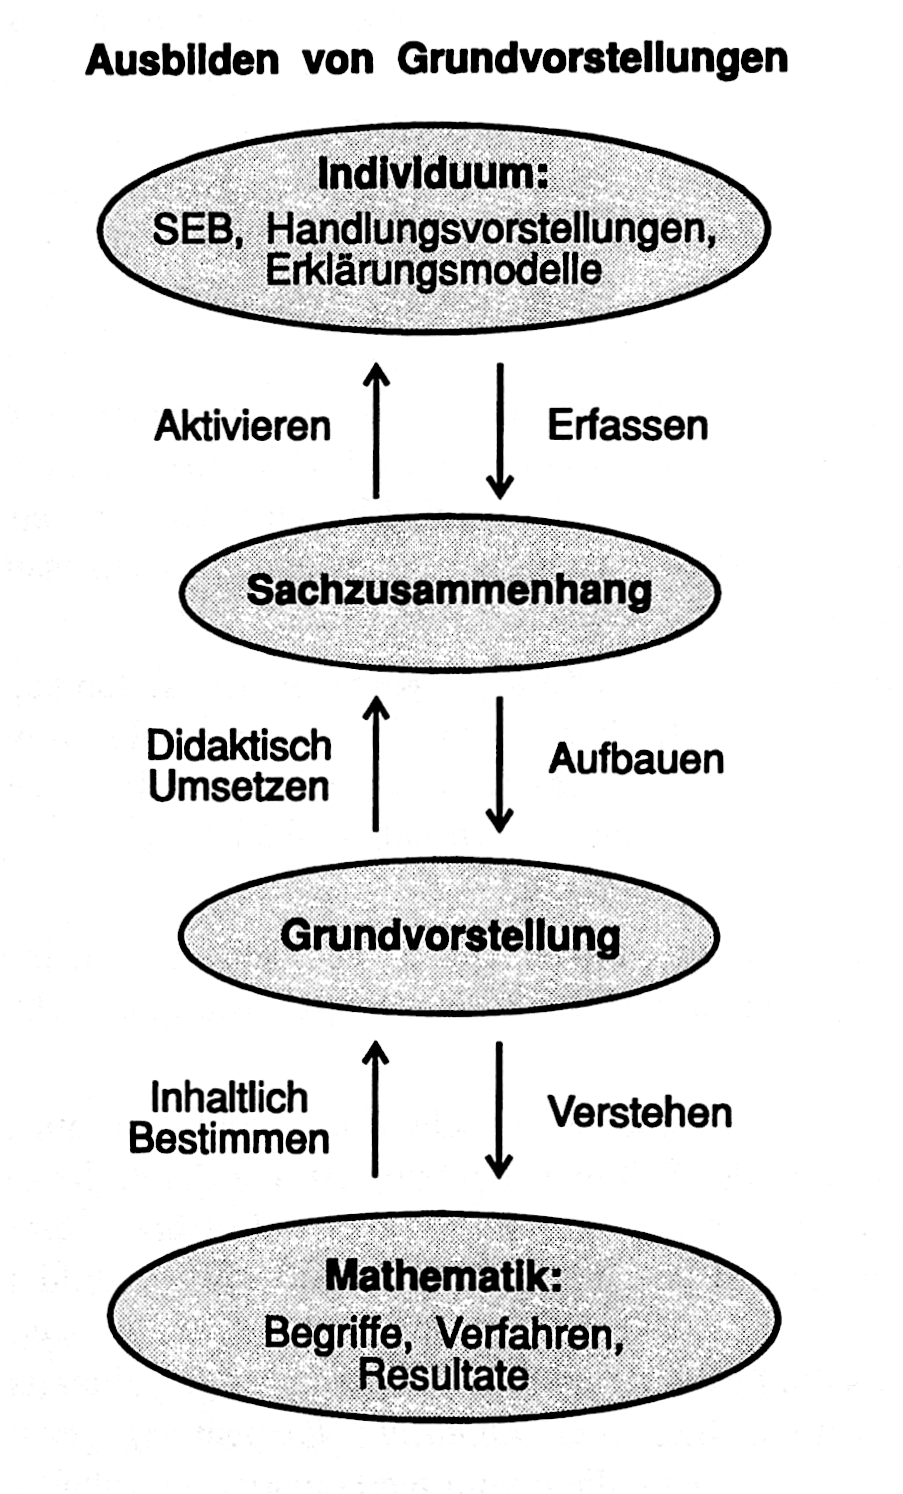
\includegraphics[width=0.5\linewidth]{pictures/4-GVausbilden} 

}

\caption{Ausbilden von Grundvorstellungen (\protect\hyperlink{ref-Hofe:1995}{vom Hofe, 1995, S. 124})}\label{fig:GVausbilden}
\end{figure}

Konkreter wird es an dieser Stelle jedoch noch nicht. Im Rahmen dieser Veranstaltung werden Begriffsbildungsprozesse und die Gestaltung von Aufgaben und Lernumgebungen spätere Themen sein, so dass darüber dann auch die \textcolor{concreteColor}{konkrete Ebene} des Vier-Ebenen-Ansatzes zur stoffdidaktischen Analyse beleuchtet wird.

\hypertarget{beispiele}{%
\section{Beispiele}\label{beispiele}}

\hypertarget{natuxfcrliche-zahlen}{%
\subsection{Natürliche Zahlen}\label{natuxfcrliche-zahlen}}

Betrachten Sie folgenden (fiktiven) Zeitungsartikel:

\begin{quote}
\textbf{\emph{Harlequin erneut auf dem 1. Platz}}

\emph{Bei dem traditionellen Pferderennen am 15. Mai hat das Pferd Harlequin erneut gewonnen. Unter den 10 Pferden, die an den Start gingen, belegte es mit 21,3 Sekunden den 1. Platz. Damit war es fast 2 mal so schnell unterwegs wie das letzte Pferd, das ins Ziel kam. Karten für das nächste Rennen können unter 030 23125143 bestellt werden.}
\end{quote}

In dem Text tauchen Zahlen unter vielen Aspekten auf: Der \textbf{1.} Platz und \textbf{15.} Mai sind \textbf{Ordinalzahlen}, also Zahlen, die eine Ordnung beschreiben. Wie oben schon beschrieben, lassen diese sich fachmathematisch über die Peano-Axiome beschreiben und wenn mit ihnen gerechnet, entspricht z.~B. das Addieren dem \textbf{Weiterzählen}.

Die \textbf{10} Pferde stellen eine \textbf{Kardinalzahl} dar, also die Anzahl der Elemente einer Menge. Addiert man Kardinalzahlen, so müssen \textbf{Mengen vereinigt} werden, z.~B. anschaulich, indem man sie zusammen legt.

Die \textbf{21,3} Sekunden entsprechen einer \textbf{Maßzahl}, da diese Zahl die Funktion hat, etwas auszumessen (hier die Zeit). Das Addieren in diesem Aspekt entspräche dem \textbf{Aneinanderlegen}, z.~B. wenn zwei Längenangaben addiert werden.

Dass es \textbf{2} mal so schnell wird, enspricht einem \textbf{Operatoraspekt}, mit dem die Vielfachheit eines Vorganges beschrieben wird. Das Addieren ist hierin eine \textbf{Hinereinanderausführung} eines Vorganges.

Die Telefonnumer \textbf{030 23125143} wiederum erfüllt einen \textbf{Codierungsaspekt}. Sie hat im mathematischen Sinne keine Bedeutung, nur die Anordnung der Ziffern ist von Relevanz. Entsprechend kann innerhalb dieses Aspektes auch nicht addiert werden. Weitere Beispiele hierfür wären Postleitzahlen oder Identifikationsnummern.

Hinzu kommt noch der Aspekt der \textbf{Rechenzahl}. Informationen dazu sowie eine genauere Erläuterung der Zahlaspekte und damit verbundenen Operationen findet man z.~B. bei \protect\hyperlink{ref-Krauthausen:2018}{Krauthausen} (\protect\hyperlink{ref-Krauthausen:2018}{2018, S. 43~ff.}).

\hypertarget{bruchzahlen}{%
\subsection{Bruchzahlen}\label{bruchzahlen}}

Nachdem die Schülerinnen und Schüler ihr gesamte Vorschul- und Primarstufenzeit mit Natürlichen Zahlen verbracht haben, treten mit der Einführung von Bruchzahlen Umbrüche in den subjektiven Vorstellungen auf. Zum Beispiel sind folgende (vermeintlichen) Gesetzmäßigkeiten plötzlich \emph{nicht mehr} gültig:

\begin{itemize}
\tightlist
\item
  Das Produkt zweier Zahlen ist größer als die jeweiligen Faktoren.
\item
  Die Multiplikation kann als wiederholte Addition aufgefasst werden.
\item
  Jede Zahl hat genau einen Repräsentanten.
\item
  Je mehr Stellen eine Zahl hat, desto größer ist sie.
\end{itemize}

Die Bruchzahlen selbst besitzen nach \protect\hyperlink{ref-Padberg:2017}{Padberg \& Wartha} (\protect\hyperlink{ref-Padberg:2017}{2017, S. 19~ff.}) folgende Aspekte:

\begin{itemize}
\tightlist
\item
  Bruch als \textbf{Anteil eines Ganzen} oder \textbf{mehrerer Ganzer}
  (z.~B. \(\frac{2}{3}\) als zwei Drittel einer Pizza oder je ein Drittel von zwei Pizzen)
\item
  Bruch als \textbf{Maßzahl}
  (z.~B. \(\frac{1}{4}\) Liter)
\item
  Bruch als \textbf{Operator}
  (z.~B. \(\frac{1}{5}\) von 250 €)
\item
  Bruch als \textbf{Verhältnis}
  (z.~B. \(\frac{2}{3}\) mit der Bedeutung \emph{2 von 3 Schüler/-innen tragen eine Brille})
\item
  Bruch als \textbf{Quotient}
  (z.~B. \(\frac{3}{5}\) als Ergebnis bzw. andere Schreibweise von \(3:5\))
\item
  Bruch als \textbf{Lösung einer linearen Gleichung}
  (z.~B. \(\frac{3}{5}\) als Lösung von \(5x = 3\))\\
\item
  Bruch als \textbf{Skalenwert}
  (z.~B. \(\frac{3}{2}\) als Mitte zwischen \(1\) und \(2\) auf dem Zahlenstrahl)
\item
  \textbf{Quasikardinale Auffassung} von Brüchen
  (z.~B. \(\frac{3}{5}\) als 3 mal \(\frac{1}{5}\))
\end{itemize}

Neben den Grundrechenoperationen führt auch das Vergleichen von Brüchen zu Grundvorstellungsumbrüchen. Hinzu kommen noch besondere Operationen mit Bruchzahlen wie das Erweitern und Kürzen.

Das Multiplizieren von Brüchen kann bspw. als Anteilsbildung (\(\frac{1}{5}\) mal \ldots{} heißt \(\frac{1}{5}\) \emph{von} \ldots) oder als Rechteckfläche aufgefasst werden (\protect\hyperlink{ref-Padberg:2017}{Padberg \& Wartha, 2017, S. 108~ff}), siehe Abbildung \ref{fig:Bruchmultiplikation}.

\begin{figure}

{\centering 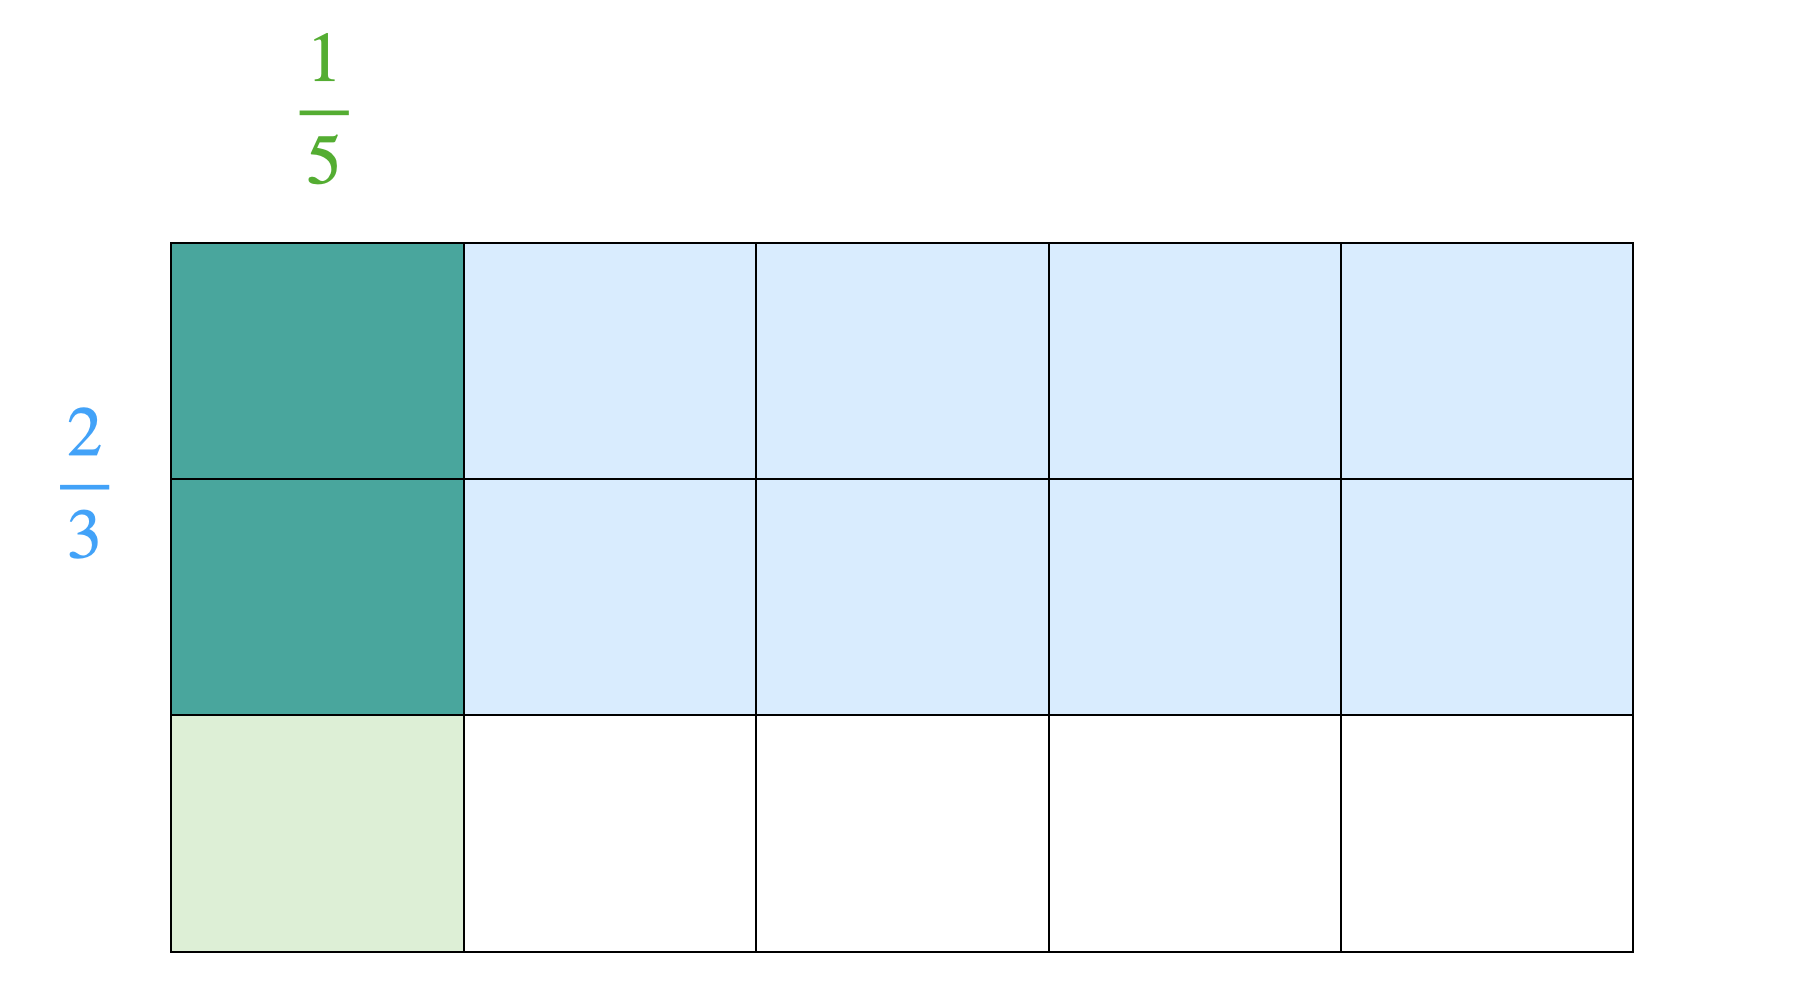
\includegraphics[width=0.5\linewidth]{pictures/4-Bruchmulti} 

}

\caption{Vorstellung von $\frac{1}{5} \cdot \frac{2}{3}$ als Rechteckfläche}\label{fig:Bruchmultiplikation}
\end{figure}

All dies zeigt, dass Brüche behutsam unterrichtet werden sollten und von einer rein kalkülorientierten Behandlung unbedingt abgesehen werden muss, da diese den nachhaltigen Lernerfolg deutlich mindert.

\hypertarget{grundvorstellungen-nachbereitung}{%
\section{Zum Nachbereiten}\label{grundvorstellungen-nachbereitung}}

\begin{enumerate}
\def\labelenumi{\arabic{enumi}.}
\tightlist
\item
  Lesen Sie (mindestens) die Kapitel 1.11.2, 1.11.4., 2.1, 2.2 und 2.4 des Buches \emph{Grundvorstellungen mathematischer Inhalte} (\protect\hyperlink{ref-Hofe:1995}{vom Hofe, 1995}).
\item
  Wählen Sie eine Grundvorstellung zu einem mathematischen Begriff aus und arbeiten Sie an dieser die Grundvorstellungsidee nach Definition \ref{def:Grundvorstellungen} durch, d.~h.

  \begin{itemize}
  \tightlist
  \item
    stellen Sie die Sinnhaftigkeit des Begriffs durch mögliche Handlungserfahrungen dar,\\
  \item
    finden Sie geeignete Repräsentationen, anhand derer operatives Handeln ermöglicht wird und\\
  \item
    beschreiben Sie mögliche Modellierungsprozesse des Begriffs mithilfe der gewählten Grundvorstellung.
  \end{itemize}
\item
  Wiederholen Sie Aufgabe 2 an weiteren Begriffen.
\end{enumerate}

\hypertarget{erstes-intermezzo-flaecheninhalt}{%
\chapter{Erstes Intermezzo: Flächeninhalt}\label{erstes-intermezzo-flaecheninhalt}}

\begin{quote}
\textbf{Lernziele}

\begin{itemize}
\tightlist
\item
  Sie vertiefen Ihr Verständnis über den Vier-Ebenen-Ansatz, insbesondere auf der formalen und semantischen Ebene.
\item
  Sie verknüpfen Ihr Wissen über Fundamentale Ideen und Grundvorstellungen am Beispiel des Flächeninhaltsbegriffs.
\end{itemize}

\textbf{Material}

\begin{itemize}
\tightlist
\item
  Folien zur Vorlesung zum Ersten Intermezzo (\href{files/Stoffdidaktik-WiSe2122-Kap5.pdf}{pdf}, \href{files/Stoffdidaktik-WiSe2122-Kap5.key}{Keynote})
\end{itemize}
\end{quote}

In diesem Kapitel werden Fundamentale Ideen und Grundvorstellungen im Zusammenhang mit dem Flächeninhaltsbegriff diskutiert. Ein Schulbuchkapitel zum Flächeninhaltsbegriff bietet die Motivation, die \textcolor{formalColor}{formale} und \textcolor{semanticColor}{semantische} Ebene des \protect\hyperlink{tab:fragen-ebenen}{Vier-Ebenen-Ansatzes} zu diskutieren und einen ersten Ausblick auf die \textcolor{concreteColor}{konkrete} und \textcolor{empiricColor}{empirische} Ebene zu geben.

In dem Sinne wird also existierendes Material analysiert und hinsichtlich der mathematikdidaktischen Theorie reflektiert. Ein solches Vorgehen wäre auch für Ihren Seminarvortrag bzw. die Hausarbeit im Rahmen dieser Veranstaltung möglich -- dann natürlich etwas ausführlicher, als hier dargestellt.

\hypertarget{darstellung-im-schulbuch}{%
\section{Darstellung im Schulbuch}\label{darstellung-im-schulbuch}}

In dem Schulbuch \emph{Mathewerkstatt} (\protect\hyperlink{ref-Barzel2012}{Barzel et al., 2012c}) wird der Flächeninhalt über den Kontext von Tiergehen eingeführt (siehe Abbildung \ref{fig:Tiergehege}). So haben in einem Zoo verschiedene Tiere unterschiedlich große Gehe zur Verfügung. Die Form der Gehege variiert dabei ebenfalls.



\begin{figure}

{\centering 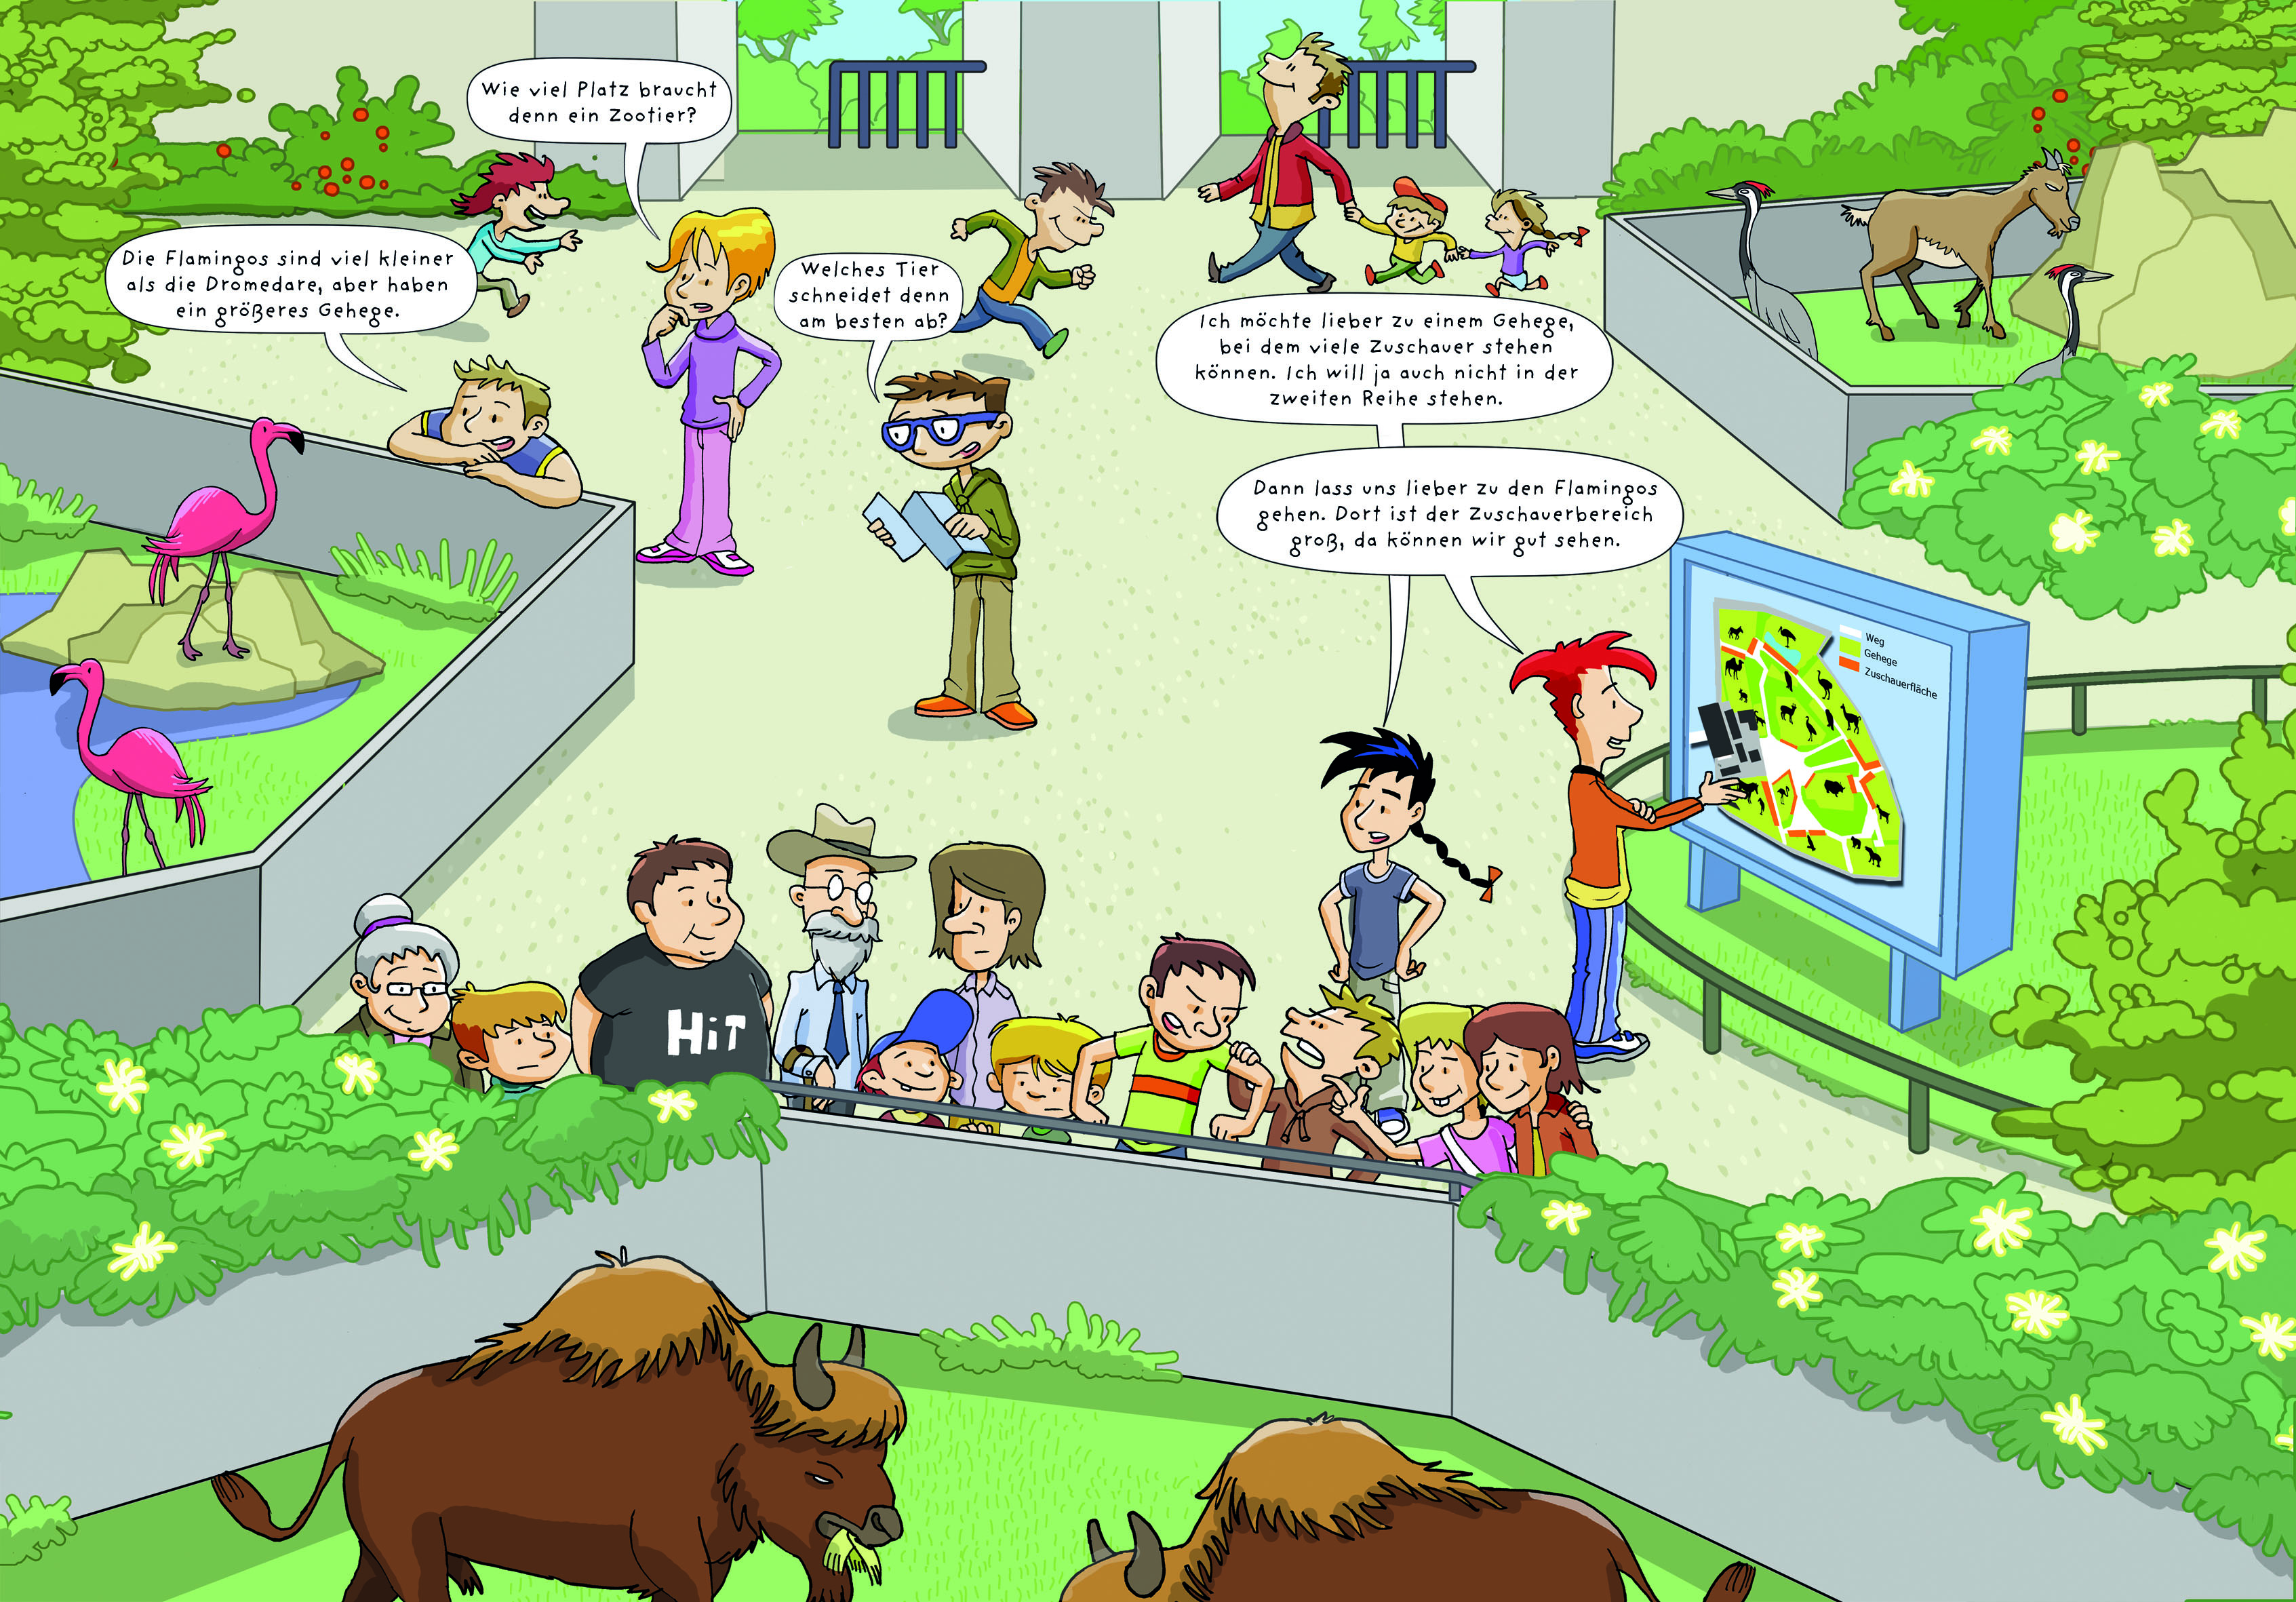
\includegraphics[width=1\linewidth]{pictures/5-Tiergehege} 

}

\caption{Einstiegsbild zum Thema Flächeninhalt (\protect\hyperlink{ref-Barzel2012}{Barzel et al., 2012c, S. 168~f.})}\label{fig:Tiergehege}
\end{figure}

Die Schülerinnen und Schüler werden nun in einer Erkundungsphase vor die Aufgabe gestellt, die Gehegegrößen miteinander zu vergleichen sowie möglichst geschickt die Größe eines Geheges messen zu können.

Anschließend erfolgen Ordnungs- und Vertiefungsphasen, in denen das Wissen struktruiert und geübt wird. Das Schulbuch wird durch einen Materialblock begleitet (\protect\hyperlink{ref-Barzel2012b}{Barzel et al., 2012b}), was in diesem Fall insbesondere dem Auseinanderschneiden und Zusammenlegen bzw. dem Auslegen von Flächen dienen soll. Weiterhin gibt es für Lehrerinnen und Lehrer ein ausführliches Begleitmaterial (\protect\hyperlink{ref-Barzel2012a}{Barzel et al., 2012a}), in dem alle Seiten des Schulbuches sowie fachdidaktische Hintergründe zur Thematik erläutert sind.

\hypertarget{formale-ebene-1}{%
\section{Formale Ebene}\label{formale-ebene-1}}

\begin{quote}
Welche Begriffe und Sätze sollen erarbeitet werden?\\
Welche Verfahren sollen erarbeitet werden und wie werden sie formal begründet?\\
Wie lassen sich die Begriffe, Sätze, Begründungen und Verfahren logisch strukturieren?\\
Welche Verbindungen zwischen den Fachinhalten sind entscheidend, welche weniger bedeutsam?\\
Wie kann das Netzwerk aus Begriffen, Sätzen, Begründungen und Verfahren entwickelt werden?
\end{quote}

Fachmathematisch kann der Flächeninhalt einer Figur als ein \textbf{nichtnegatives Maß} aufgefasst werden, wobei zwei \textbf{zueinander kongruenten Figuren dasselbe Maß} zugeordnet wird und der Flächeninhalt einer Figur gleich der \textbf{Summe der Flächeninhalte ihrer Teilfiguren} ist, sofern zerlegbar. Hinzu wird das Flächeninhaltsmaß eines Quadrates der Seitenlänge 1~LE auf 1~LE2 festgelegt (vgl. \protect\hyperlink{ref-Kuntze2018}{Kuntze, 2018, S. 161}).

Dies ist eine \textbf{axiomatische Herangehensweise}, die sich für Schülerinnen und Schüler in der Regel als herausfordernd darstellt (\protect\hyperlink{ref-Kuntze2018}{Kuntze, 2018, S. 162}). Häufig wird eine umschreibende Definition genutzt, wie: \emph{Der Flächeninhalt einer Fläche gibt an, wie groß diese ist.} Dabei ist jedoch die mögliche Mehrdeutigkeit dieser Formulierung zu beachten -- so könnte auch der Umfang einer Figur als Maß für ihre \emph{Größe} aufgefasst werden, da der Größenbegriff in dem Fall unspezifisch ist.

Ob nun eine explizite Definition gewählt wird oder nicht -- dies ist auch abhängig von der persönlichen Einstellung der Lehrkraft und den Voraussetzungen der Lerngruppe -- in jedem Fall ist ein tragfähiges mathematisches Verständnis aufzubauen. Hierzu können die in den Axiomen enthaltenen Eigenschaften über sinnvolle \textbf{Lernhandlungen} aufgebaut werden (siehe auch \protect\hyperlink{ref-Worner2014}{Wörner, 2014, S. 1328~f.}):

\begin{itemize}
\tightlist
\item
  Vergleichen verschiedener Flächen durch Zerlegen, Ergänzen und Übereinanderlegen
\item
  Bestimmen des Maßes einer Fläche über Auszählen mittels eines Vergleichsmaßes
\item
  Nutzen eines quadratischen Vergleichsmaßes, in der Regel 1~cm2
\end{itemize}

All diese Überlegungen kommen zunächst \textbf{ohne Formeln} aus, weshalb diese im Unterricht auch erst im Anschluss an eine inhaltliche Erarbeitung des Flächeninhaltsbegriffs eingeführt und genutzt werden sollten.

Fachsystematisch entscheidend ist, dass ein \textbf{Flächenvergleich zunächst ohne ein explizites Maß} möglich ist -- hierfür reichen die Kongruenzeigenschaft und das Zerlegen/Ergänzen von Flächen aus. Das Vergleichsmaß ist dann relevant, wenn man den \textbf{Flächeninhalt mithilfe einer Zahl objektivieren} bzw. ohne eine explizite Vergleichsfigur auskommen möchte.

Interessant ist hier auch die \textbf{\emph{Willkürlichkeit} des Vergleichsmaßes}. Kulturell geprägt ist hier (in Kontinentaleuropa) zwar beispielsweise 1~cm2, aber auch andere Einheiten sind gleichberechtigt möglich. Auch muss das Vergleichsmaß nicht zwingend ein Quadrat sein. Nicht selten wird z.~B. von großen Flächen angegeben, wie viele Fußballfelder in sie hineinpassen würden. Für den Unterricht bedeutet das, dass im Sinne einer auf den mathematischen Kern orientierten Sichtweise zunächst möglichst allgemeine und vielfältige (auch \emph{unförmige}) Vergleichsflächen herangezogen werden können. Später ist dann natürlich ein Bezug zu den Standardeinheiten herzustellen (siehe Abbildung \ref{fig:FlaecheEinheiten}).



\begin{figure}

{\centering 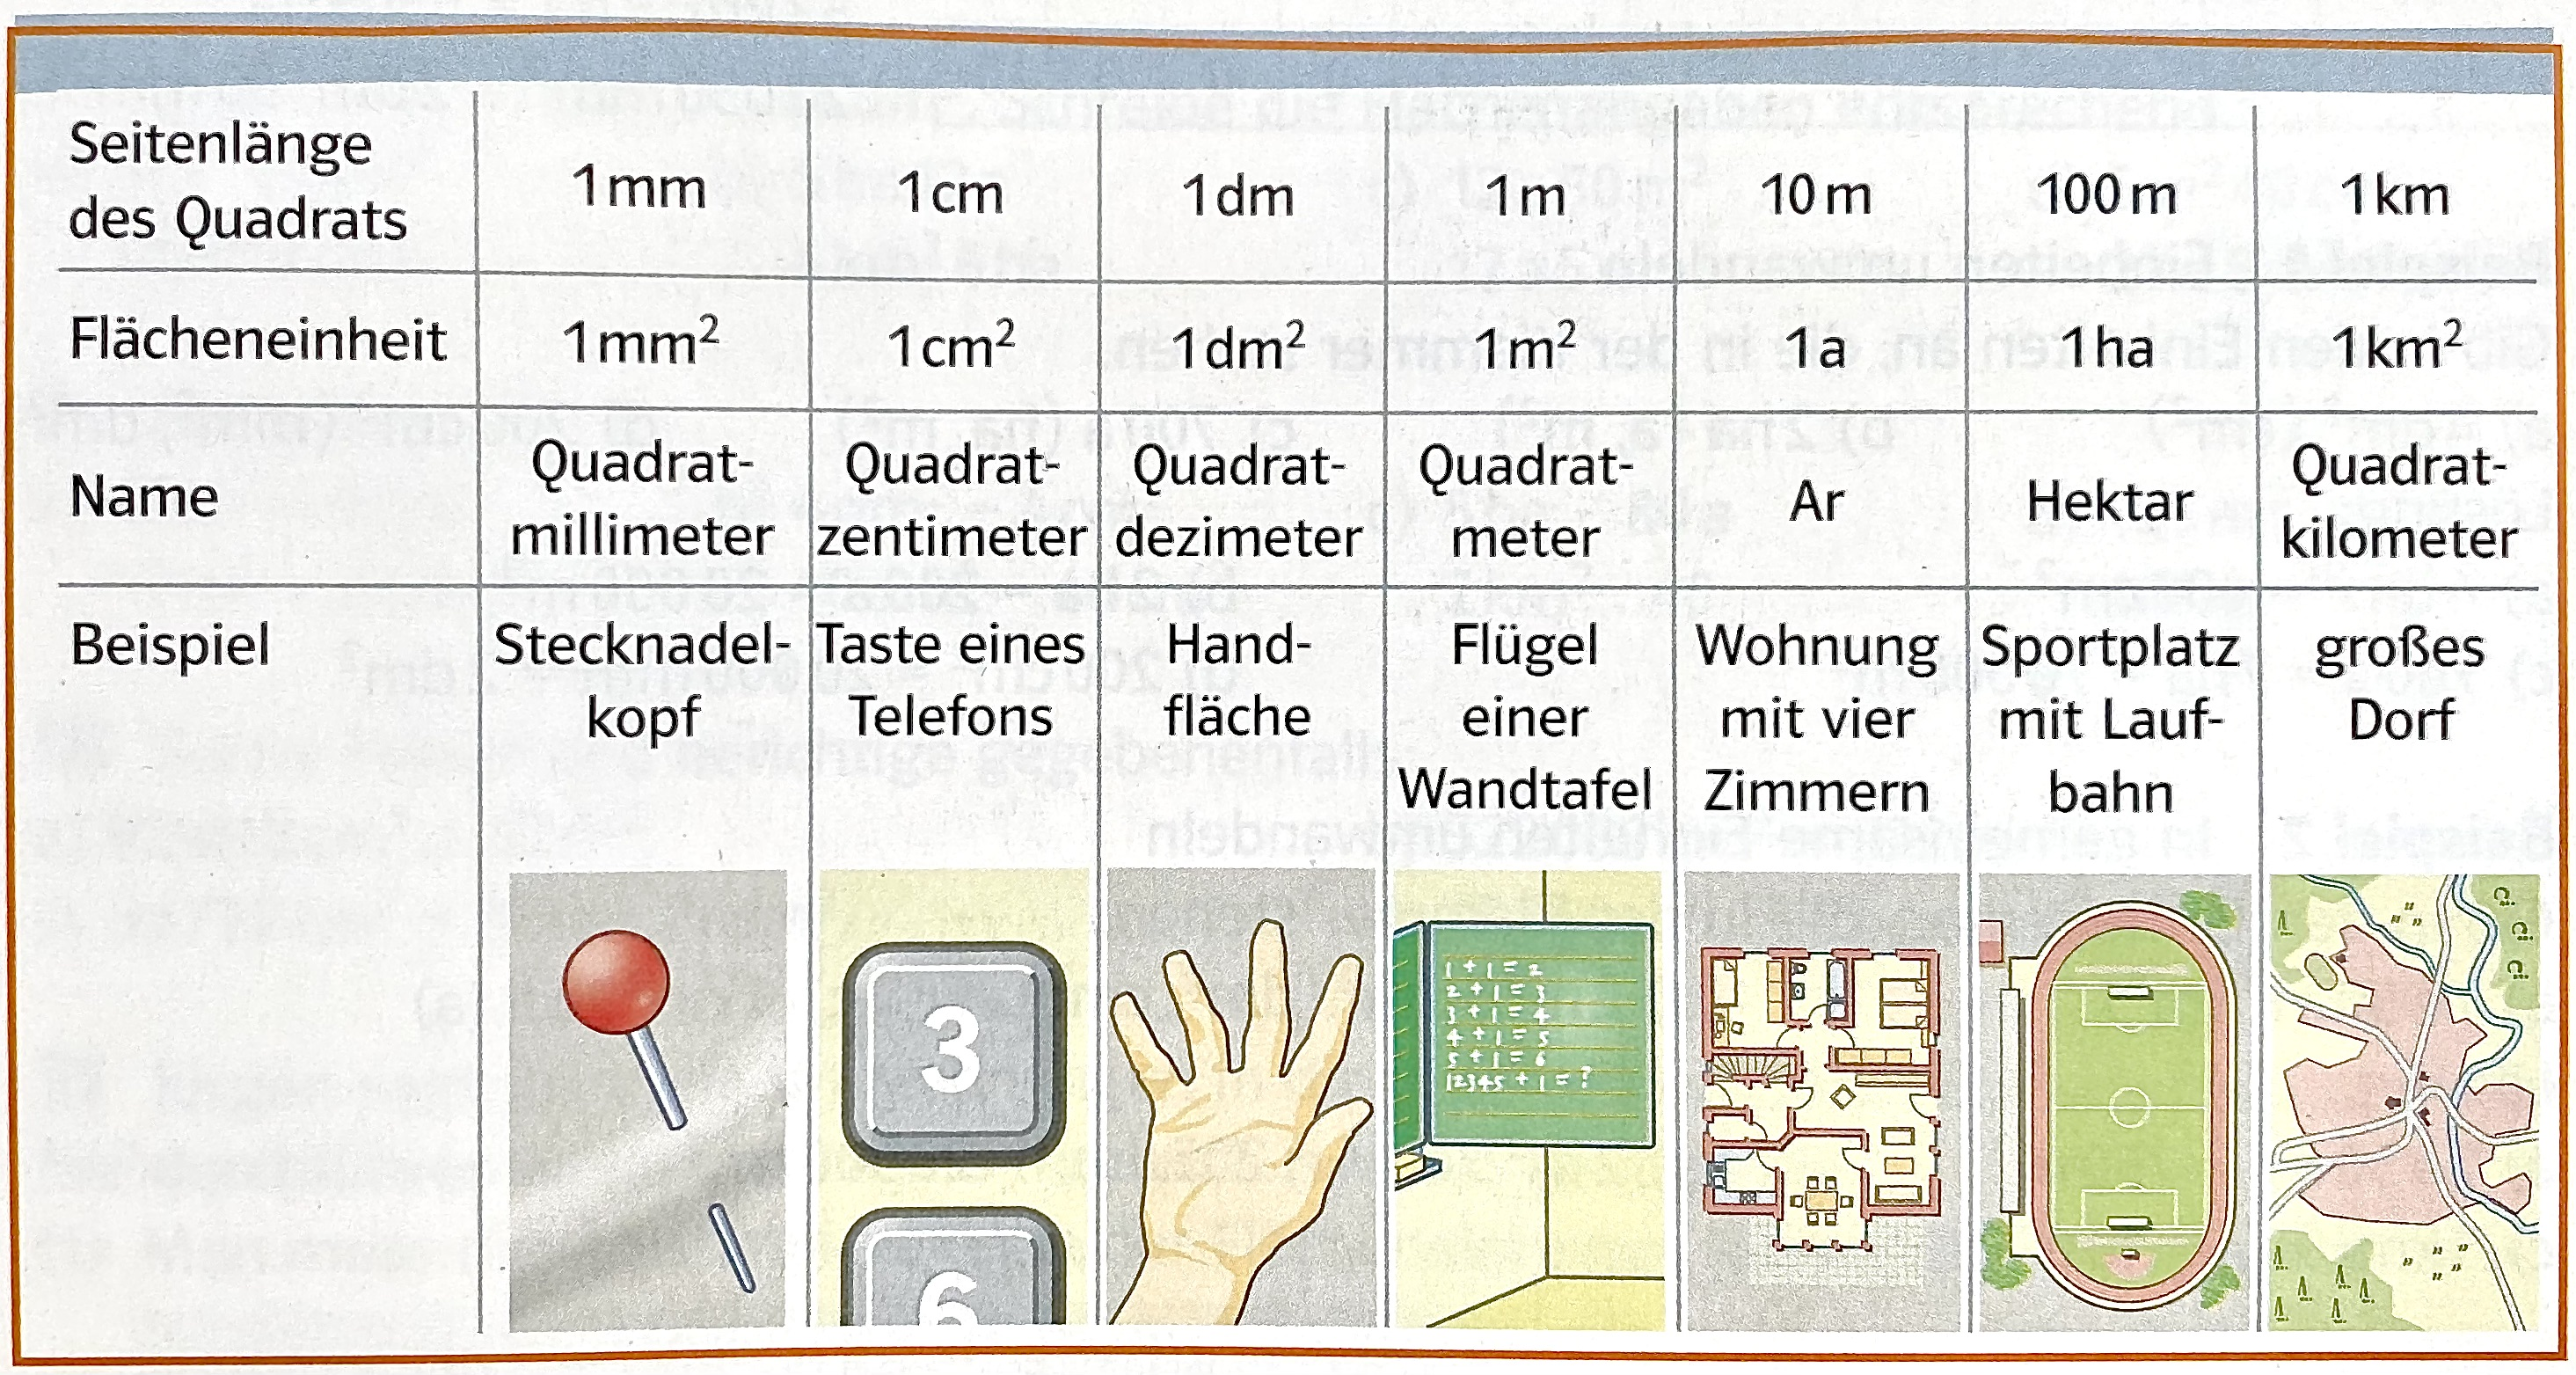
\includegraphics[width=0.75\linewidth]{pictures/5-Einheiten} 

}

\caption{Standardeinheiten typischer Vergleichsflächen (\protect\hyperlink{ref-Lambacher2010}{\emph{Lambacher {Schweizer} {Mathematik} für {Gymnasien}. 5, {Schülerbuch}}, 2010, S. 193})}\label{fig:FlaecheEinheiten}
\end{figure}

\hypertarget{semantische-ebene-1}{%
\section{Semantische Ebene}\label{semantische-ebene-1}}

\begin{quote}
Welche Fundamentalen Ideen liegen hinter den Begriffen, Sätzen und Verfahren?\\
Welche Grundvorstellungen und Repräsentationen (graphisch, verbal, numerisch und algebraisch) sind für den Verständnisaufbau entscheidend?\\
Wie verhalten sich Ideen und Vorstellungen zueinander und zu früheren und späteren Lerninhalten?\\
Wie kann ein Lernpfad angeordnet werden, in dem das Verständnis, zusammen mit den Erkenntnissen der formalen Ebene, aufgebaut wird?
\end{quote}

\hypertarget{fundamentale-idee-messen}{%
\subsection{Fundamentale Idee Messen}\label{fundamentale-idee-messen}}

Dem Flächeninhaltsbegriff liegt zweifelsohne die Fundamentale Idee des \emph{Messens} zugrunde. \protect\hyperlink{ref-Vohns:2000}{Vohns} (\protect\hyperlink{ref-Vohns:2000}{2000, S. 52~ff.}) stellt ausführlich dar, warum das Messen als Fundamentale Idee aufgefasst werden kann, worauf in diesem Abschnitt Bezug genommen wird. Besondere Betonung legt \protect\hyperlink{ref-Vohns:2000}{Vohns} (\protect\hyperlink{ref-Vohns:2000}{2000, S. 49}) darauf, dass Messen »der indirekte Vergleich von Objekten in bezug {[}sic{]} auf eine bestimmte Eigenschaft« ist.

\emph{Horizontal} zieht sich dies über viele Gebiete der Mathematik hinweg (z.~B. Messprozesse in der Geometrie, Maßzahlaspekt von Brüchen in der Arithmetik, Erwartungswert als Lagemaß in der Stochastik, Integral in der Analysis), aber auch darüber hinaus ist das Messen von hoher Relevanz (z.~B. Messprozesse in der Physik, quantitative Studien in den Sozialwissenschaften, Pulsmessung in der Medizin). Damit wird auch das \emph{Sinnkriterium} der Fundamentalen Idee offensichtlich.

Das \emph{Vertikalkriterium} zeigt sich beispielsweise in der Längenbestimmung in der Grundschule, Flächeninhaltsbestimmung in der Orientierungsstufe, bei Verwandlungen von Flächen (z.~B. beim Beweis des Satzes des Pythagoras) bzw. der Approximation von Flächen (z.~B. Bestimmen des Kreisflächeninhalts) bis hin zum Integralbegriff als verallgemeinerter Flächeninhalt.

\emph{Historisch} ist das Messen ebenfalls in vielen Epochen der Mathematik bedeutsam, worauf typische Wortwendungen wie \emph{Alles ist Zahl!} (bei den Pythagoräern), \emph{Die Vermessung der Welt} (mit der Methode der Triangulation) oder die \emph{Quadratur des Kreises} (als klassisches Problem der Geometrie) hindeuten. Auch die Vereinheitlichung von Maßeinheiten (z.~B. SI-Einheiten) zeigt die Bedeutsamkeit des Messens für die wissenschaftliche Entwicklung.

\hypertarget{gv-zum-fluxe4cheninhalt}{%
\subsection{GV zum Flächeninhalt}\label{gv-zum-fluxe4cheninhalt}}

Die folgenden Überlegungen sind empirisch nicht abgesichert, sondern vorwiegend theoretischer Natur. Ansatzpunkt ist ein Beitrag von \protect\hyperlink{ref-Worner2014}{Wörner} (\protect\hyperlink{ref-Worner2014}{2014}). Setzt man die dortigen Darstellungen genauer mit der Definition \ref{def:Grundvorstellungen} von Grundvorstellungen in Bezug, lassen sich (meiner Meinung nach) Grundvorstellungen zu drei Aspekten des Flächeninhaltsbegriffs formulieren:

\begin{itemize}
\tightlist
\item
  \textbf{Maßzahlaspekt}: Flächeninhalt einer Figur als nichtnegative Maßzahl, die mittels normierter Flächeninhaltsmaße bestimmt wird
\item
  \textbf{Vereinigungsaspekt}: Flächeninhalt einer Figur als Summe der Flächeninhalte der Teilfiguren, aus denen sich die Figur zusammensetzen lässt
\item
  \textbf{Kongruenzaspekt}: Flächeninhalt einer Figur als invariante Eigenschaft gegenüber Kongruenzabbildungen
\end{itemize}

Für jeden dieser Aspekte sollen nun Handlungserfahrungen, Repräsentationen und mögliche Anwendungen auf die Realität diskutiert werden. Weiterhin werden einige Operationen mit Flächeninhalten besprochen.

\hypertarget{mauxdfzahlaspekt}{%
\subsubsection{Maßzahlaspekt}\label{mauxdfzahlaspekt}}

Eine Erfahrung, die die Grundvorstellung zu diesem Aspekt stützt, ist das Auslegen von Flächen mittels normierter Flächenstücke, wie z.~B. Quadrate. Hieraus kann die Erfahrung gewonnen werden, dass die Anzahl der Quadrate direkt den Flächeninhalt (mit der entsprechenden Einheit) angibt.

Als Repräsentation kann hierfür einfaches Kästchenpapier dienen, auf das die auszumessende Fläche gemalt wird (siehe Abbildung \ref{fig:FlaecheMasszahl}). Daran kann man das Abzählen der normierten Flächenstücke durchführen bzw. sich vorstellen. Insbesondere können daran auch Verfeinerungen (und damit genaueres Messen) nachvollzogen werden.

\begin{figure}

{\centering 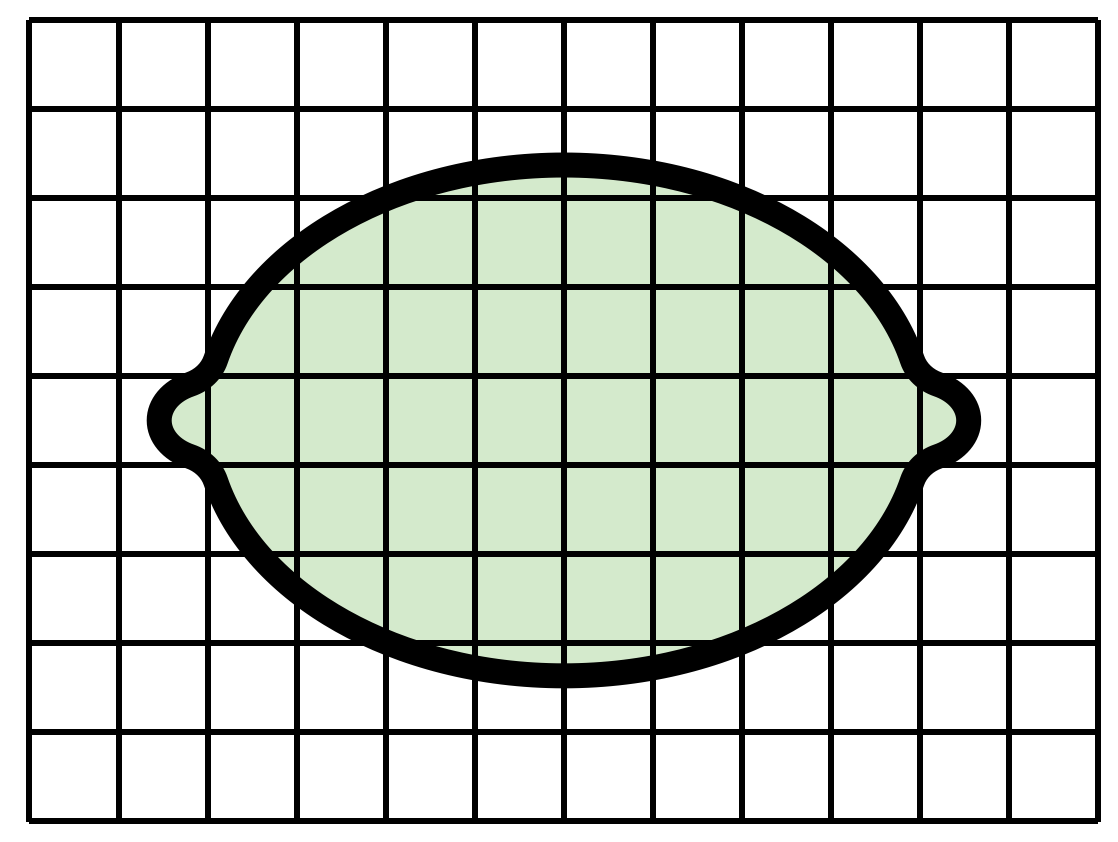
\includegraphics[width=0.25\linewidth]{pictures/5-Masszahl} 

}

\caption{Repräsentation des Maßzahlaspektes}\label{fig:FlaecheMasszahl}
\end{figure}

Eine mögliche Anwendung in der Realität ist das Bestimmen der Größe eines Fußballfeldes. Hier kann man die Länge und Breite in Metern messen, um zu bestimmen, wie viele Quadratmeter in das Feld passen. Dies wird dann zwar nicht über tatsächliches Auslegen realisiert, aber es wird (bei Verwendung der Rechteckinhaltsformel) auf die entsprechende Vorstellung Bezug genommen.

\hypertarget{vereinigungsaspekt}{%
\subsubsection{Vereinigungsaspekt}\label{vereinigungsaspekt}}

Zur Grundvorstellung des Vereinigungsaspektes gehört die Erfahrung, Flächen auseinanderzuschneiden und neu zusammenzulegen, um ihren Flächeninhalt bestimmen bzw. die Größe zweier Flächen miteinander vergleichen zu können.

Die Schnittlinien können bspw. durch gestrichelte Linien repräsentiert werden, so dass die Handlungserfahrung hier in der Vorstellung nachvollzogen werden kann (siehe Abbildung \ref{fig:FlaecheVereinigung}).

\begin{figure}

{\centering 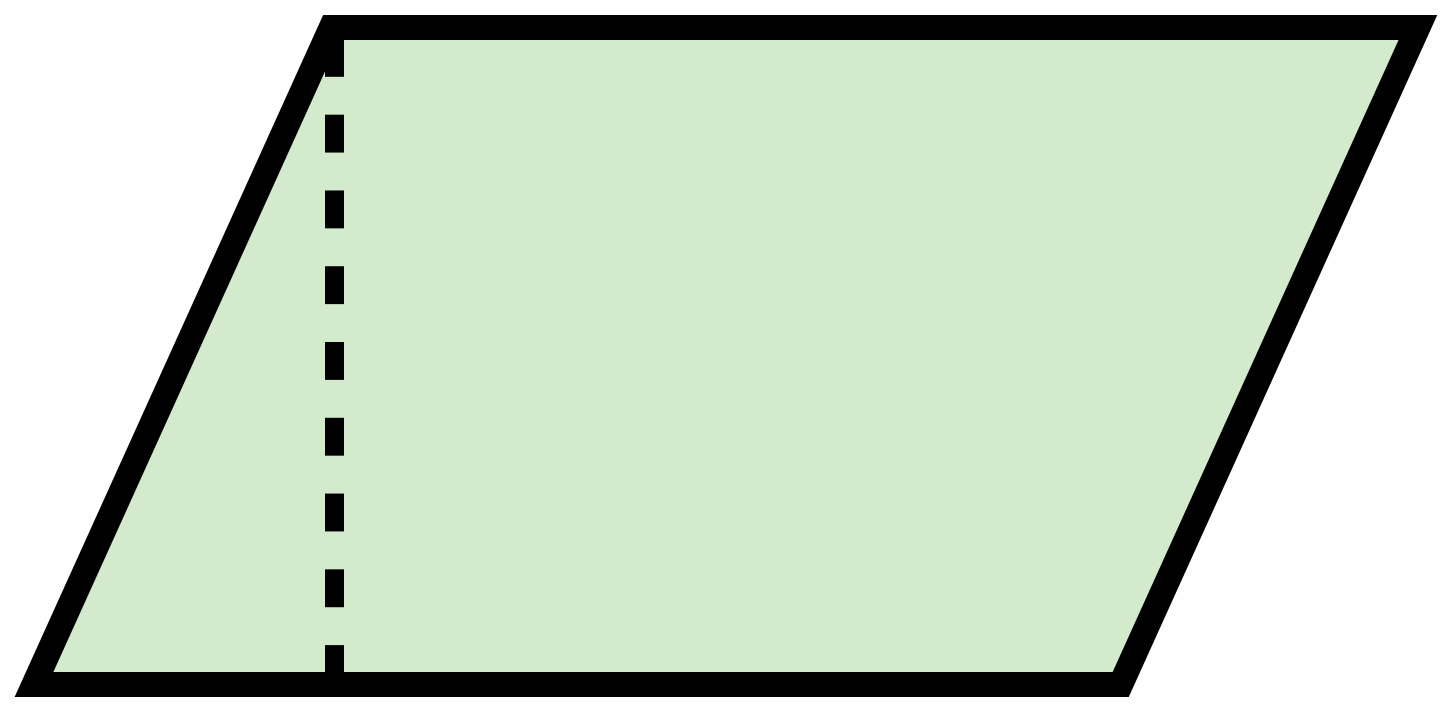
\includegraphics[width=0.25\linewidth]{pictures/5-abb-Vereinigung} 

}

\caption{Repräsentation des Vereinigungsaspektes}\label{fig:FlaecheVereinigung}
\end{figure}

Möchte man die Größe eines Landes bestimmen, so ist es in der Regel notwendig, dieses in geeignete Flächenstücke zu zerlegen, deren Flächeninhalte einfacher berechnet werden können. Dies ist also eine mögliche Anwendung in der Realität. Je nach Komplexität der Figur (und ggf. zusätzlichen geometrischen Überlegungen) können so auch Flächeninhaltsformeln gefunden werden (was schon eine innermathematische Anwendung ist).

\hypertarget{kongruenzaspekt}{%
\subsubsection{Kongruenzaspekt}\label{kongruenzaspekt}}

Wer hat größere Hände? Um diese Frage zu beantworten, ist eine typische Erfahrung, die Hände aneinanderzulegen und ihre Größen zu vergleichen. Dabei wird die Vorstellung genutzt, dass zueinander kongruente Figuren den gleichen Flächeninhalt haben.

Eine Repräsentation, die dabei unterstützt, im Kongruenzaspekt zu operieren, kann in der Teilung oder \emph{Ummantelung} von Figuren mittels zueinander kongruenter Figuren liegen (siehe Abbildung \ref{fig:FlaecheKongruenz}). Dies ist z.~B. bei der Herleitung der Flächeninhaltsformel für ein Dreieck sinnvoll, um zu erkennen, dass dieser der Hälfte des Flächeninhalts des umschriebenen Rechtecks entspricht\footnote{Um diesen Zusammenhang vollumfänglich zu verstehen, sind weiterhin der Vereinigungsapekt (Aufteilen in Teildreiecke) und der Maßzahlaspekt (um die Flächeninhaltsformel fürs Rechteck zu verstehen) nötig.}.

\begin{figure}

{\centering 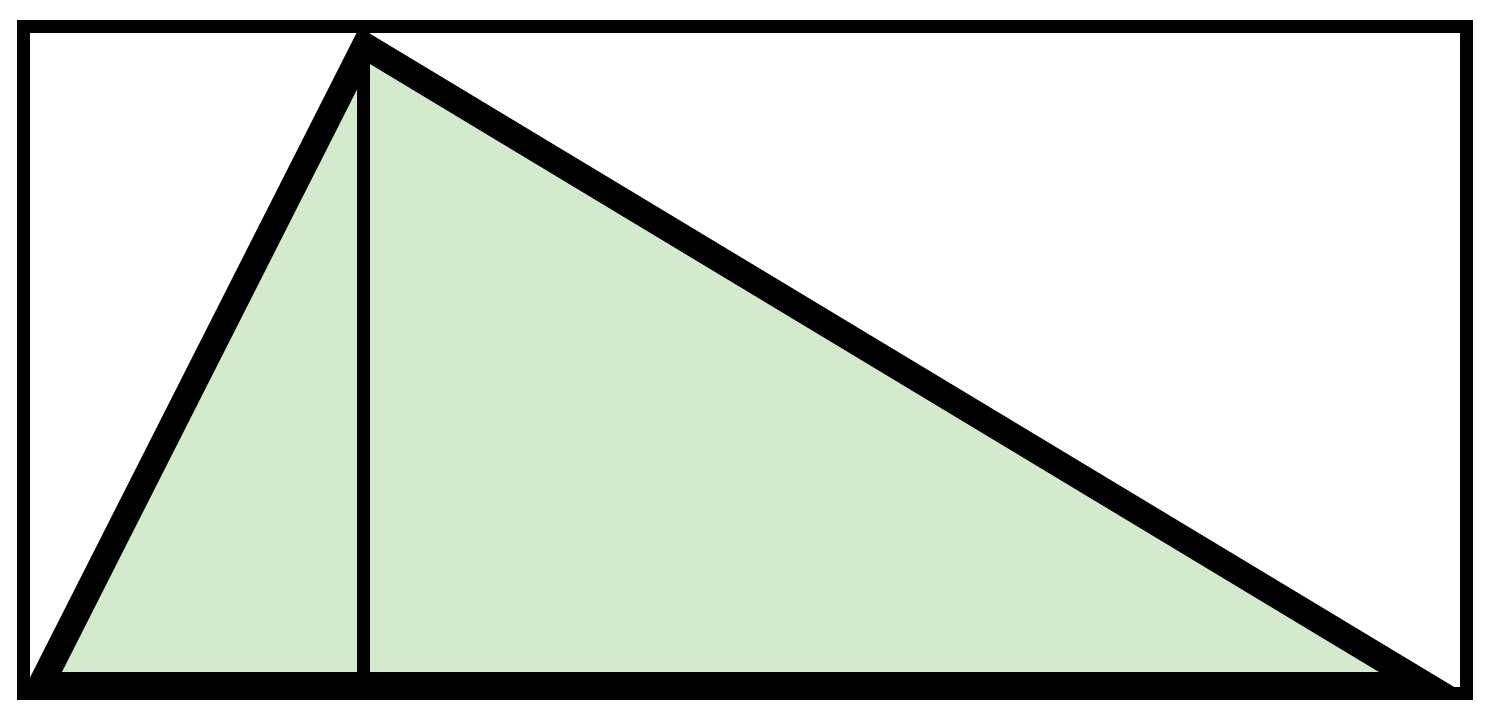
\includegraphics[width=0.25\linewidth]{pictures/5-Kongruenz} 

}

\caption{Repräsentation des Kongruenzaspektes}\label{fig:FlaecheKongruenz}
\end{figure}

Eine (innermathematische) Anwendung dieser Vorstellung könnte zum Beispiel bei der Berechnung des Oberflächeninhalts eines Primas liegen, wo die Flächeninhalte von Grund- und Deckfläche i.~d.~R. nicht einzeln berechnet werden, sondern einer der Flächeninhalte wegen der Kongruenz einfach verdoppelt wird.

\hypertarget{operieren-mit-fluxe4cheninhalten}{%
\subsubsection{Operieren mit Flächeninhalten}\label{operieren-mit-fluxe4cheninhalten}}

Für unterschiedliche Operationen, die mit Flächeninhalten durchgeführt werden, können nun in unterschiedlicher Weise die Grundvorstellungen zu den Aspekten aufgegriffen und genutzt werden:

\begin{itemize}
\tightlist
\item
  Um Flächeninhalte direkt miteinander zu \textbf{vergleichen}, sind der Vereinigungs- und Kongruenzaspekt relevant, da die Flächen ggf. neu aufgeteilt werden müssen und dann mittels Übereinanderlegen gegeneinander abgeschätzt werden können.
\item
  Um die \textbf{Flächeninhaltsformel eines Rechtecks} zu begründen, benötigt es den Maßzahlaspekt, da das Abzählen einbeschriebener Vergleichsquadrate wesentlich ist. Dies hängt auch eng mit der Grundvorstellung der Multiplikation als Rechteckflächeninhalt zusammen (siehe Abbildung \ref{fig:Bruchmultiplikation}).
\item
  Für die \textbf{Flächeninhaltsformel des Dreiecks} sind wieder Kongruenz- und Vereinigungsaspekt relevant, da das Dreieck geeignet zerlegt und mit dem umschriebenen Rechteck verglichen werden muss (siehe Abbildung \ref{fig:FlaecheKongruenz}). Da Bezug zur Rechteckformel genommen wird, ist natürlich auch der Maßzahlaspekt relevant.
\item
  Um \textbf{Flächeninhalte zu approximieren}, wie z.~B. den eines Kreises (siehe Abbildung \ref{fig:FlaecheKreis}), benötigt es wieder alle drei Vorstellungen. So kann der Kreis in zueinander kongruente Teilflächen zerlegt werden (Kongruenz- und Vereinigungsaspekt), deren Gesamtflächeninhalt dann über die Rechteckformel näherungsweise bestimmt wird (Maßzahlaspekt).
\end{itemize}

\begin{figure}

{\centering 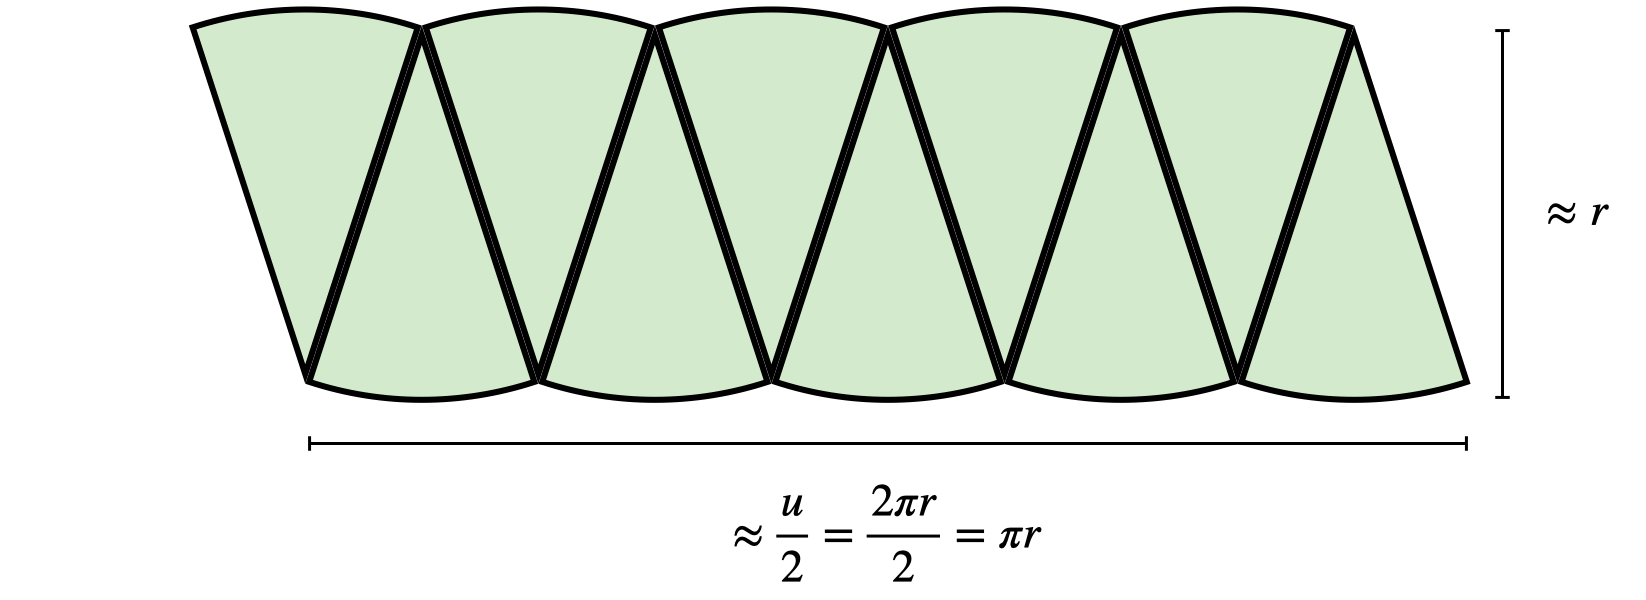
\includegraphics[width=0.75\linewidth]{pictures/5-abb-Kreis} 

}

\caption{Approximation des Kreisflächeninhalts}\label{fig:FlaecheKreis}
\end{figure}

\begin{itemize}
\tightlist
\item
  Bei der \textbf{Bestimmung von Oberflächeninhalten} von Körpern, werden der Vereinigungsaspekt für die einzelnen Seitenflächen und ggf. der Kongruenzaspekt angesprochen, wenn es zueinander kongruente Seitenflächen gibt (wie z.~B. bei Prismen), deren Flächeninhalte dann mit der entsprechenden Anzahl multipliziert und nicht einzeln ausgerechnet werden.
\end{itemize}

\hypertarget{auswirkungen-auf-lernpfad}{%
\subsection{Auswirkungen auf Lernpfad}\label{auswirkungen-auf-lernpfad}}

Der Lernpfad des Schulbuches greift diese Fundamentale Idee und die Grundvorstellungen auf, indem zunächst Flächeninhalte (durch Ausseinanderschneiden und Zusammenfügen) miteinander verglichen werden, anschließend das Auslegen mit normierten Flächenstücken erfolgt und daraufhin geeignete Maßeinheiten eingeführt werden und die Flächeninhaltsberechnung eines Rechtecks behandelt wird.

Die formale und empirische Ebenen wurden hier getrennt dargestellt, was jedoch für eine stoffdidaktische Analyse gar nicht zwingend nötig ist. Entscheidend ist, dass Sie den ganzheitlichen Blick auf die aufgeworfenen Fragen haben und diese (zumindest in Teilen) beantworten können. Die getrennte Darstellung dient hier noch der Übersicht für Sie als \emph{Anfängerinnen und Anfänger} im Umgang mit stoffdidaktischen Analysen -- auch wenn darauf verzichtet wurde, die einzelnen Fragen schrittweise explizit zu beantworten.

\hypertarget{ausblick-auf-konkrete-ebene}{%
\section{Ausblick auf konkrete Ebene}\label{ausblick-auf-konkrete-ebene}}

\begin{quote}
Welche Kernfragen und Kernideen können die Entwicklung der Begriffe, Sätze und Verfahren leiten?\\
Welche Kontexte und Probleme sind geeignet, um an ihnen die Kernfragen und -ideen exemplarisch zu behandeln und die Inhalte zu rekonstruieren?\\
Wie kann das Verständnis sukzessive über konkrete Situationen in den beabsichtigten Lernpfaden konstruiert werden (horizontale Mathematisierung)?\\
Wie können die Lernpfade in Bezug auf die Problemstruktur angeordnet werden (vertikale Mathematisierung)?
\end{quote}

Als \textbf{Kontext} wählt das Schulbuch den Platzbedarf bei \textbf{Tiergehegen im Zoo.} Dieser Kontext ist aus mehreren Gründen besonders gut geeignet:

\begin{itemize}
\tightlist
\item
  In der Regel interessiert tatsächlich nur der Flächeninhalt des Geheges. Inhaltliche Verwechslungen mit dem Umfang oder dem Volumen können damit reduziert werden.\\
\item
  Es ist aus dem Kontext heraus sinnstiftend, die Größe der Gehege miteinander zu vergleichen, da verschiedene Tiere einen unterschiedlichen Platzbedarf haben.\footnote{Verwiesen wird auch auf ein \emph{Gutachten über Mindestanforderungen an die Haltung von Säugetieren} vom \protect\hyperlink{ref-BundesministeriumfurErnahrungundLandwirtschaft2014}{Bundesministerium für Ernährung und Landwirtschaft} (\protect\hyperlink{ref-BundesministeriumfurErnahrungundLandwirtschaft2014}{2014}).}
\item
  Verschiedene Formen der Tiergehege lassen sich nutzen, um verschiedene Vergleichsstrategien zu motivieren. So können z.~B. Flächen zerlegt und neu zusammengesetzt werden, runde Formen angenähert werden und durch das Ausschneiden der Figuren ist ein Übereinanderlegen möglich.
\end{itemize}

Dabei werden zwei \textbf{Kernideen} aufgegriffen (\protect\hyperlink{ref-Barzel2012a}{Barzel et al., 2012a, S. 359~f.}):

\begin{itemize}
\tightlist
\item
  Eine besteht im \textbf{Vergleich der Flächeninhalte} der verschiedenen Gehege. Dieses aus dem Kontext heraus begründbare Vorgehen führt im mathematischen Sinne zum Bedürfnis, Flächen zu vermessen, um sie miteiander vergleichen zu können.\\
\item
  Die zweite Kernidee ist das \textbf{geschickte Bestimmen eines Flächeninhalts}, wofür zunächst mittels Kästchenpapier das Auszählen von Flächen mit unterschiedlicher Genauigkeit diskutiert wird, anschließend geeignete Maßeinheiten eingeführt werden und die Flächeninhaltsformel des Rechtsecks behandelt wird.
\end{itemize}

Diese Ideen werden jeweils über die Prozesse des Erkunden, Ordnens und Vertiefens realisiert. Durch dieses Vorgehen\footnote{\protect\hyperlink{ref-Prediger2014}{Prediger et al.} (\protect\hyperlink{ref-Prediger2014}{2014}) bezeichnen diese Prozesse auch als \emph{Kernprozesse} des Unterrichtens.} wird das Verständnis sukzessive aufgebaut. Es wird Bestandteil der weiteren Veranstaltung der Stoffdidaktik sein, wie zu mathematischen Inhaltsbereichen geeignete Kontexte und Kernideen bzw. Kernfragen gefunden werden können, die den Lernpfad anschließend leiten.

\hypertarget{ausblick-auf-empirische-ebene}{%
\section{Ausblick auf empirische Ebene}\label{ausblick-auf-empirische-ebene}}

\begin{quote}
Welche typischen individuellen Voraussetzungen (Vorstellungen, Kenntnisse, Kompetenzen, \ldots) sind zu erwarten und wie passen diese zum angestrebten Verständnis (Ressourcen vs.~Hindernisse)?\\
Woher kommen typische Hindernisse oder unerwünschte Vorstellungen?\\
Wie können typische Vorkenntnisse und Vorstellungen als fruchtbare Anknüpfungspunkte dienen?\\
Welche Schlüsselstellen (Hindernisse, Wendepunkte, \ldots) gibt es im Lernweg der Schülerinnen und Schüler?\\
Wie kann der angestrebte Lernpfad bezüglich der Anknüpfungspunkte und Schlüsselstellen neu angeordnet werden?
\end{quote}

\protect\hyperlink{ref-Kuntze2018}{Kuntze} (\protect\hyperlink{ref-Kuntze2018}{2018, S. 159~f.}) verweist auf typische Schwierigkeiten von Schülerinnen und Schülern im Umgang mit dem Flächeninhaltsbegriff.

So kommt es häufig zu einer Verwechslung zwischen Längenmaßen, Flächeninahlten und Volumina. Eine Ursache wird v.~a. in der frühzeitigen kalkülhaften Herangehensweise gesehen, Flächeninhalte über Formeln berechnen zu müssen. So fehlt ein tiefergehendes Begriffsverständnis und die Formeln können nicht sinnstiftend genutzt werden. Dem kann u.~a. dadurch begegnet werden, indem bewusst die Zusammenhänge hergestellt werden, z.~B. zwischen Umfang und Flächeninhalt.
Letztlich zeigen empirische Erhebungen, dass Kinder mit einem vertieften Verständnis über Flächeninhalte auch besser in der Lage sind, entsprechende Formeln anzuwenden (\protect\hyperlink{ref-Worner2014}{Wörner, 2014, S. 1330}).

Weiterhin besteht wegen der Wortverwandtschaft von \emph{Fläche} und \emph{Flächeninhalt} die Gefahr, dass entsprechende Vorstellungen nicht aufgebaut werden, insbesondere dann, wenn die Begriffe (zumindest von der Lehrkraft) nicht sauber getrennt verwendet werden. Die Fläche ist die Figur an sich und wird über ihre \emph{Form} bestimmt. Der Flächeninhalt ist ein \emph{Maß} für die Größe der Figur (vgl. \protect\hyperlink{ref-Barzel2012a}{Barzel et al., 2012a, S. 362}). Insbesondere für Schülerinnen und Schüler, deren Muttersprache nicht Deutsch ist, kann die fehlerhafte Verwendung dieser feinen Unterschiede hinderlich dabei sein, dem Unterricht zu folgen.

Derartige Schwierigkeiten werden im Schulbuch implizit aufgegriffen (z.~B. strikte sprachliche Trennung) oder explizit thematisiert (z.~B. verbindende und vergleichende Behandlung mit dem Umfang von Figuren), so dass auch dies wieder die Gestaltung des Lernpfades beeinflusst.

\hypertarget{erstesintermezzo-nachbereitung}{%
\section{Zum Nachbereiten}\label{erstesintermezzo-nachbereitung}}

\begin{enumerate}
\def\labelenumi{\arabic{enumi}.}
\tightlist
\item
  Diskutieren Sie zu weiteren typischen Operationen mit Flächeninhalten, welche Grundvorstellungen dafür aufgegriffen und genutzt werden.
\item
  Finden Sie einen alternativen Kontext (statt den Zoogehegen), der geeignet ist, die Kernideen so aspektreich durchzuarbeiten.
\end{enumerate}

\hypertarget{part-konkrete-ebene}{%
\part*{Konkrete Ebene}\label{part-konkrete-ebene}}
\addcontentsline{toc}{part}{Konkrete Ebene}

\hypertarget{begriffsbildung}{%
\chapter{Begriffsbildung}\label{begriffsbildung}}

\begin{quote}
\textbf{Lernziele}

\begin{itemize}
\tightlist
\item
  Sie kennen Kriterien für das Verständnis von Begriffen.
\item
  Sie kennen Wege der Begriffseinführung und wählen diese zielgerichtet aus -- auch abhängig von der didaktischen Funktion des jeweiligen Begriffs.
\item
  Sie können geeignete Beispiele und Gegenbeispiele auswählen und anordnen, um Begriffsbildungsprozesse zu unterstützen.
\end{itemize}

\textbf{Material}

\begin{itemize}
\tightlist
\item
  Folien zur Vorlesung zur Begriffsbildung (\href{files/Stoffdidaktik-WiSe2122-Kap6.pdf}{pdf}, \href{files/Stoffdidaktik-WiSe2122-Kap6.key}{Keynote})
\end{itemize}
\end{quote}

\hypertarget{begriffsverstuxe4ndnis}{%
\section{Begriffsverständnis}\label{begriffsverstuxe4ndnis}}

\hypertarget{begriffsbegriff}{%
\subsection{Begriffsbegriff}\label{begriffsbegriff}}

Angenommen, Sie würden eine Schülerin oder einen Schüler auffordern, den Begriff \emph{Quader} zu definieren. Die Person äußert sich, dass es sich dabei um ein Viereck mit vier gleich langen Seiten und vier rechten Winkeln handelt. Wie würden Sie da als Lehrkraft reagieren? Hat diese Person tatsächlich nicht verstanden, was ein Quader ist? Was können Sie als Lehrkraft tun, um herauszufinden, welche Wissens- oder Verständnislücken vorliegen?

Derartige Gedanken werden Ihren Schulalltag prägen, denn die \textbf{Bildung von Begriffen} ist eine der wesentlichen Aufgaben des Mathematikunterrichts. Nach \protect\hyperlink{ref-Zech1998}{Zech} (\protect\hyperlink{ref-Zech1998}{1998, S. 165}) bietet sich folgende Definition an:

\begin{definition}[Begriff]
\protect\hypertarget{def:Begriff}{}\label{def:Begriff}

Man spricht allgemein von einem »Begriff«, wenn eine Anzahl von Objekten oder Ereignissen aufgrund gewisser übereinstimmender Merkmale mit einem gemeinsamen Namen belegt wird (vgl. Weinert 1974, S. 664).

\end{definition}

Damit werden zwei Dimensionen von Begriffen sichtbar, nämlich der \textbf{Bezeichner} und das \textbf{Bezeichnete}. Während der Bezeichner das \emph{Wort} bzw. der \emph{Name} ist, mit dem das zu betrachtende Objekt oder Ereignis belegt wird, ist das Bezeichnete die \emph{Idee} hinter dem Objekt, also das Gefüge an \emph{übereinstimmenden Merkmalen}. Weder \emph{Bezeichner} noch \emph{Bezeichnetes} sind jedoch das Objekt oder Ereignis selbst.
Äquivalente, und auch in den Sprachwissenschaften bedeutsame Bezeichnungen sind \textbf{Signifikant} für den Bezeichner und \textbf{Signifikat} für das Bezeichnete (vgl. auch \protect\hyperlink{ref-Rembowski2015}{Rembowski, 2015, S. 13~ff.}; \protect\hyperlink{ref-dewiki:214582005}{Wikipedia, 2021d}, \protect\hyperlink{ref-dewiki:212433603}{2021c}).

Im obigen Beispiel hat die Schülerin oder der Schüler für den Bezeichner \emph{Quader} das Bezeichnete eines Quadrates definiert. Es kann sich hier also durchaus um eine Wortverwechslung handeln, die nicht zwingend mit einem inhaltlichen Fehlverständnis einhergehen muss.

Was heißt es nun, einen Begriff \emph{verstanden} zu haben?

Zunächst einmal müssen »Kenntnisse, Vorstellungen über sowie Fähigkeiten im Umgang mit Merkmalen oder Eigenschaften eines Begriffs und deren Beziehungen untereinander« entwickelt werden (\protect\hyperlink{ref-Weigand2015}{Weigand, 2015, S. 264}). Dies wird als ein Verständnis über den \textbf{Begriffsinhalt} bezeichnet, zu dem natürlich auch die Definition des Begriffs gehört, aber eben nicht ausschließlich.

Weiterhin ist der \textbf{Begriffsumfang} Bestandteil des Begriffsverständnisses, was heißt, »einen Überblick über die Gesamtheit aller Objekte {[}zu{]} erhalten, die unter einem Begriff zusammengefasst werden« (\protect\hyperlink{ref-Weigand2015}{Weigand, 2015, S. 264}).

Hinzu kommt das \textbf{Begriffsnetz}, über das »Beziehungen des Begriffs zu anderen Begriffen« aufgezeigt werden können (\protect\hyperlink{ref-Weigand2015}{Weigand, 2015, S. 264}).

Wenn dann noch »Kenntnisse hinsichtlich der Anwendungen des Begriffs sowie Fähigkeiten im Umgang mit dem Begriff« ausgeprägt sind und die Schülerinnen und Schüler in der Lage sind, die »Begriffsbildungen kritisch zu reflektieren« (\protect\hyperlink{ref-Weigand2015}{Weigand, 2015, S. 264}), kann von einem weitreichenden Begriffsverständnis gesprochen werden.

\hypertarget{verstuxe4ndnistiefe}{%
\subsection{Verständnistiefe}\label{verstuxe4ndnistiefe}}

Die verschiedenen mathematischen Begriffe haben eine unterschiedliche Bedeutsamkeit innerhalb der mathematischen Bildung in der Schule (und darüber hinaus). So ist offenbar der \emph{Zahlbegriff} derart fundamental und vielschichtig, dass er in allen Jahrgängen in verschiedenen Ausprägungen trägt (und nicht umsonst eine der fünf Leitideen nach den Bildungsstandards ist), während beispielsweise der Begriff \emph{Bruchstrich} als Bestandteil eines Bruches kaum weitergehende Bedeutung hat und vielmehr einer erleichternden Kommunikation dient.

\protect\hyperlink{ref-Vollrath}{Vollrath} (\protect\hyperlink{ref-Vollrath}{o.~J., S. 2}) unterscheidet dahingehend in verschiedene \emph{Didaktische Funktionen eines Begriffs} und formuliert (Hervorhebungen im Original kursiv, hier fett):

»Begriffe können als \textbf{Leitbegriffe} eines \textbf{Themenstrangs} dienen, der sich über mehrere Jahrgangsstufen erstreckt. Man denke etwa an die Begriffe Zahl, Funktion, Figur oder Abbildung.

Begriffe können als \textbf{Schlüsselbegriffe} eine \textbf{Unterrichtssequenz} strukturieren. Das kann etwa der Begriff des Bruchs für die Bruchrechnung sein, der Begriff der proportionalen Zuordnung für die Schlussrechnung, der Begriff der Symmetrie für die Lehre von den Dreiecken und Vierecken.

Ein Begriff kann \textbf{zentraler Begriff} einer \textbf{Unterrichtseinheit} sein, der in ihr erarbeitet wird. Hier ist an Begriffe zu denken wie Primzahl, Quadratwurzel, Potenzfunktion, gleichseitiges Dreieck, Kreis, Tangente, Scherung, Prisma usw.

Schließlich dienen Begriffe als \textbf{Arbeitsbegriffe} dazu, beim Arbeiten bestimmte Sachverhalte griffig zu formulieren, um über sie sprechen zu können. Hier ist an Begriffe wie Zähler, Nenner, Klammer, Grundzahl, Hochzahl, Ecke, Seite, Kante usw. zu denken.«

Offensichtlich benötigen Begriffe mit einer langfristigeren Perspektive, wie Leitbegriffe, auch ein tieferes Verständnis und damit mehr Aufmerksamkeit bei der Begriffsbildung. \protect\hyperlink{ref-Vollrath1984}{Vollrath} (\protect\hyperlink{ref-Vollrath1984}{1984, S. 215~f.}) schlägt für Leitbegriffe daher einen mehrstufigen Aufbau der Verständnistiefe vor (vgl. auch \protect\hyperlink{ref-Lechner}{Lechner, o.~J., S. 10}):

\begin{enumerate}
\def\labelenumi{\arabic{enumi}.}
\item
  \textbf{Intuitives} Begriffsverständnis (Begriff als Phänomen)

  Die Schülerinnen und Schüler entwickeln eine grundlegende Idee des Begriffs, ohne dass er für sie schon mathematisch greifbar sein muss. Der Begriff wird bspw. als Phänomen in der Umwelt erkannt oder sich ihm durch Handlungserfahrungen genähert. Diese Stufe ist also auch wesentlich, um Grundvorstellungen aufzubauen.
\item
  \textbf{Inhaltliches} Begriffsverständnis (Begriff als Träger von Eigenschaften)

  Der Begriff wird über seine Eigenschaften erfasst, ohne dass diese explizit benannt werden müssten. So können z.~B. Vorschulkinder Dreiecke und Vierecke erkennen, ohne dass ihnen eine mathematische Definition bewusst wäre. Auf dieser Stufe ist es auch schon möglich, Probleme mithilfe der Begriffseigenschaften zu lösen (z.~B. das Einsetzen entsprechender Figuren in geometrische Puzzle), ohne dass der Bezeichner des Begriffs zwingend verwendet werden muss.
\item
  \textbf{Integriertes} Begriffsverständnis (Begriff als Teil eines Begriffsnetzes)

  Der Begriff kann nun in Zusammenhang mit anderen Begriffen eines Begriffsnetzes gebracht werden. So können bspw. Gemeinsamkeiten und Unterschiede verwandter Begriffe identifiziert werden.
\item
  \textbf{Formales} Begriffsverständnis (Begriff als formales Objekt)

  Auf dieser Stufe ist für den Begriff eine mathematische Definion bekannt. So können Eigenschaften des Begriffs erläutert werden und es kann begründet werden, ob und warum einzelne Objekte zum Begriff gehören oder nicht. Der Begriff kann somit auch in Beweisen genutzt werden.
\item
  \textbf{Strukturelles} Begriffsverständnis (Begriff als strukturierbares Objekt)

  Der Begriff kann nun als Strukturobjekt aufgefasst werden, so dass er selbst wieder Anlass für mathematische Untersuchungen ist. Beim Funktionsbegriff heißt dies z.~B., dass Verknüpfungen zwischen Funktionen hergestellt werden oder Darstellungsformen miteinander in Bezug gebracht werden können.
\end{enumerate}

Zumindest die ersten drei Stufen sind auch für kurz- und mittelfristig auszuprägende Begriffe relevant (vgl. \protect\hyperlink{ref-Weigand2015}{Weigand, 2015, S. 273~ff.}).

\hypertarget{wege-zum-begriff}{%
\section{Wege zum Begriff}\label{wege-zum-begriff}}

\hypertarget{arten-der-begriffseinfuxfchrung}{%
\subsection{Arten der Begriffseinführung}\label{arten-der-begriffseinfuxfchrung}}

Die Einführung von Begriffen kann stets als Wechselspiel zwischen \textbf{Beispielen/Gegenbeispielen} und der \textbf{Begriffsfestlegung} aufgefasst werden. Je nachdem, in welcher Richtung und Qualität dieser Zusammenhang erbracht wird, spricht man von einer \textbf{ostensiven}, \textbf{induktiven} oder \textbf{deduktiven} Begriffseinführung (siehe Abbildung \ref{fig:Begriffseinfuehrung}).

\begin{figure}

{\centering 
\includegraphics[width=0.75\linewidth]{pictures/6-Begriffe} 

}

\caption{Möglichkeiten der Begriffseinführung}\label{fig:Begriffseinfuehrung}
\end{figure}

Neben diesen drei Grundformen gibt es auch noch Abwandlungen und Abweichungen, wie z.~B. das Aufsteigen vom Abstrakten zum Kokreten (siehe Abschnitt \ref{aufsteigen-vom-abstrakten-zum-konkreten}) oder die Operative Genese in der Geometrie (siehe Abschnitt \ref{bonus-operative-genese}).

\hypertarget{ostensive-begriffseinfuxfchrung}{%
\subsubsection{Ostensive Begriffseinführung}\label{ostensive-begriffseinfuxfchrung}}

Bei der ostensiven Begriffseinführung wird das Lernen eines Begriffs als \textbf{Erfassen der Gestalt} als einprägsames Ganzes angenommen. Das heißt, der Begriff wird gar nicht formal definiert, sondern nur über Beispiele dargestellt. Dies wird insbesondere bei Arbeitsbegriffen so gehandhabt (z.~B. \emph{Bruchstrich}) oder bei der Begriffseinführung in der Grundschule, wenn deren Gestalt leicht eingänglich ist (z.~B. \emph{Kreis}).

Dabei muss jedoch die \textbf{wahrgenommene Gestalt dem Wesentlichen} des Begriffs entsprechen und der \textbf{Gestalteindruck ist häufig abhängig von der Lage}. Es ist also darauf zu achten, nicht ausschließlich Spezialfälle zu präsentieren, die dann zu einer Untergeneralisierung des Begriffs führen. Werden z.~B. zwei \emph{zueinenander senkrechte} Strecken präsentiert, sollten diese also nicht gleich lang sein, sich nicht in der Mitte schneiden und auch nicht parallel zu den Tafel-/Blatt-/Bildschirmrändern ausgerichtet sein (siehe Abbildung \ref{fig:SenkrechtOstensiv}).



\begin{figure}

{\centering 
\includegraphics[width=0.5\linewidth]{pictures/6-senkrecht} 

}

\caption{Ungeeignete und geeignete ostensive Darstellung des Begriffs \emph{senkrecht zueinander}}\label{fig:SenkrechtOstensiv}
\end{figure}

\hypertarget{induktive-begriffseinfuxfchrung}{%
\subsubsection{Induktive Begriffseinführung}\label{induktive-begriffseinfuxfchrung}}

Bei der induktiven Begriffseinführung wird zunächst eine \textbf{Vielzahl an Beispielen} präsentiert. Aus diesen heraus wird dann das \textbf{Wesentliche des Begriffs extrahiert}. Dafür werden die Objekte zunächst beschrieben und anschließend gemeinsame Eigenschaften entdeckt. Dies kann passieren, indem die ungeordneten Beispiele nach Merkmalen sortieren werden oder bereits in Teilmengen aufgeteilt präsentiert werden. Daran wird nun der Begriffsinhalt herausgearbeitet.

Dieses Vorgehen ist relativ natürlich, da es auch der Begriffsbildung im Vorschulalter bzw. im Alltag entspricht. Allerdings benötigt es sehr viel Zeit. Hinzu kommt, dass das Erkennen der gemeinsamen Merkmale in der Unterrichtssituation nicht selten zu einem \emph{Ostereiersuchen} verfällt, indem die Lehrkraft so lange nachfragt, bis die gewünschte Eigenschaft gefunden wird. Oder noch kritischer formuliert: »Die Lernenden jedoch haben noch keine Ahnung von diesem Wesen und können sie auch nicht gewinnen, da sie keinerlei Mittel dafür besitzen.« (\protect\hyperlink{ref-Giest2004a}{Giest \& Lompscher, 2004})

Beim Einsatz der induktiven Begriffseinführung müssen also insbesondere geeignete Impulsfragen im Vorhinein bedacht werden, um die Schülerinnen und Schüler durch gezielte Fragestellungen das Wesentliche des Begriffs entdecken lassen zu können.

\hypertarget{deduktive-begriffseinfuxfchrung}{%
\subsubsection{Deduktive Begriffseinführung}\label{deduktive-begriffseinfuxfchrung}}

Die deduktive Begriffseinführung geht den Weg \textbf{von der Definition zu den Beispielen}. Dieses Vorgehen ist das übliche in der Hochschulmathematik und sollte -- um zum Beispiel wissenschaftspropädeutisch tätig zu sein -- auch im Schulunterricht schon vermittelt werden.

Typische Lernhandlungen im Zusammenhang mit deduktiver Begriffseinführung sind das \textbf{Identifizieren} (d.~h. anhand existierender Objekte die Begriffszugehörigkeit entscheiden) und \textbf{Realisieren} (d.~h. Herstellen) von Repräsentanten\footnote{Diese \emph{Repräsentanten} eines Begriffs sind nicht mit dessen \emph{Repräsentationen} im Sinne der Grundvorstellungsidee zu verwechseln! Die Repräsentanten sind konkrete (reale oder ideelle) Objekte, Repräsentationen dagegen Darstellungen, die ein operatives Arbeiten ermöglichen. Beides kann aber natürlich sehr ähnlich aussehen oder sogar zusammenfallen.} des Begriffs und das \textbf{Begründen} der Begriffszugehörigkeit.

Typische Impulsfragen für den Unterricht, um die deduktive Begriffseinführung nach Gabe der Definition zu unterstützen, können sein:

\begin{itemize}
\tightlist
\item
  Ist das ein \ldots?
\item
  Stelle ein \ldots{} her.
\item
  Welche Teile der Definition sind nicht erfüllt?
\item
  Was muss an dem \ldots{} verändert werden, damit es ein \ldots{} ist?
\item
  Wie prüft man, ob das ein \ldots{} ist?
\item
  Warum entsteht ein \ldots, wenn man das so und so herstellt?
\end{itemize}

\hypertarget{beispiele-und-gegenbeispiele}{%
\subsection{Beispiele und Gegenbeispiele}\label{beispiele-und-gegenbeispiele}}

Unabhängig davon, auf welche Art und Weise man Begriffe einführt, ist stets ein Zusammenspiel aus Beispielen, Gegenbeispielen und verbalen Erläuterungen notwendig -- und das in allen Altersklassen! Bei entsprechenden Verbalisierungen sind ggf. weniger Beispiele/Gegenbeispiele nötig, da damit das Wesen des Begriffs besser herausgearbeitet werden kann (\protect\hyperlink{ref-Zech1998}{Zech, 1998, S. 260}).

Bei der Auswahl von Beispielen und Gegenbeispielen bieten sich das \textbf{Variationsprinzip} und das \textbf{Kontrastprinzip} an. Die folgenden Überlegungen stammen hauptsächlich von \protect\hyperlink{ref-Zech1998}{Zech} (\protect\hyperlink{ref-Zech1998}{1998, S. 260~ff.}).

\hypertarget{variationsprinzip}{%
\subsubsection{Variationsprinzip}\label{variationsprinzip}}

Beispiele sollten breit variiert werden, es darf nicht zu einer Untergeneralisierung kommen. Im Alltag als Gegenbeispiele empfundene Beispiele müssen mit angebracht werden. Wichtig erscheinende \textbf{irrelevante Merkmale} sollten mindestens einmal \textbf{variiert} werden.

Für den Rechtecktbegriff kann dies eine Variation in Größe, Seitenverhältnis, Ausrichtung und Farbe, aber auch die Präsentation von Spezialfällen (z.~B. eines Quadrates) bedeuten (siehe Abbildung \ref{fig:VariationRechteck}).



\begin{figure}

{\centering 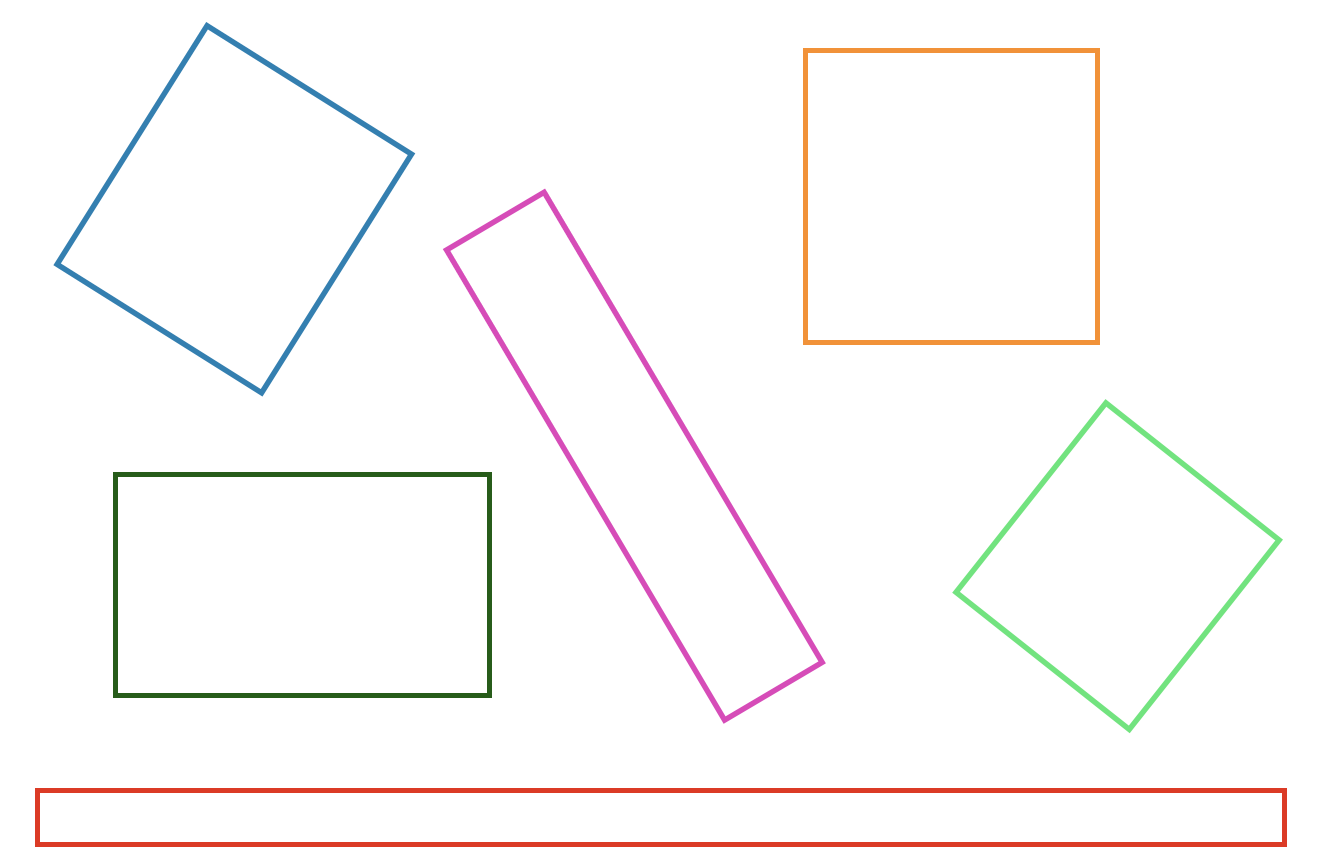
\includegraphics[width=0.75\linewidth]{pictures/6-Variation} 

}

\caption{Variationsprinzip beim Begriff \emph{Rechteck}}\label{fig:VariationRechteck}
\end{figure}

Um dieses Prinzip für einen Begriff zu realisieren, muss man sich als Lehrkraft also Gedanken über die mathematisch relevanten und irrelevanten Eigenschaften machen. Auch eine explizite Diskussion mit den Schülerinnen und Schüler, warum diese Eigenschaften variiert werden durften (und andere nicht), kann hilfreich für das Begriffsverständnis sein.

\hypertarget{kontrastprinzip}{%
\subsubsection{Kontrastprinzip}\label{kontrastprinzip}}

Gegenbeispiele dürfen nicht für Beispiele gehalten werden, es darf nicht zu einer Übergeneralisierung kommen. Im Alltag als Beispiele empfundene Gegenbeispiele (sogenannte \emph{Fastbeispiele}) müssen diskutiert werden. \textbf{Relevante Merkmale} müssen mindestens einmal \textbf{fehlen}.

Für den Rechteckbegriff relevant sind etwa die rechten Winkel (was bei Beibehaltung der gleich langen, parallelen Seiten zu einem Parallelogramm führt). Auch die \emph{Ecken}-Eigenschaften und die Tatsache, dass es sich um eine Figur (und nicht um einen Körper) handelt, sind relevant (siehe Abbildung \ref{fig:KontrasRechteck}).



\begin{figure}

{\centering 
\includegraphics[width=0.5\linewidth]{pictures/6-Kontrast} 

}

\caption{Kontrastprinzip beim Begriff \emph{Rechteck}}\label{fig:KontrasRechteck}
\end{figure}

\hypertarget{darbietung-von-beispielen-und-gegenbeispielen}{%
\subsubsection{Darbietung von Beispielen und Gegenbeispielen}\label{darbietung-von-beispielen-und-gegenbeispielen}}

\protect\hyperlink{ref-Zech1998}{Zech} (\protect\hyperlink{ref-Zech1998}{1998, S. 261}) fasst zusammen: \textbf{»Beispiele und Gegenbeispiele sind dann am effektivsten, wenn sich die Beispiele möglichst stark in den irrelevanten Merkmalen unterscheiden und die Gegenbeispiele in möglichst wenigen relevanten Merkmalen unterscheiden.«}

Eine simultane Darbietung zweier stark kontrastierender Beispiele (Abbildung \ref{fig:SimultanBeispiel}) oder eines Beispiels mit einem sehr ähnlichen Gegenbeispiel (Abbildung \ref{fig:SimultanGegenbeispiel}) kann weiterhin den Fokus auf die relevanten Merkmale des Begriffs lenken.



\begin{figure}

{\centering 
\includegraphics[width=0.5\linewidth]{pictures/6-Quadrat} 

}

\caption{Simultane Darbietung zweier Beispiele zum Begriff \emph{Quadrat}}\label{fig:SimultanBeispiel}
\end{figure}



\begin{figure}

{\centering 
\includegraphics[width=0.4\linewidth]{pictures/6-Achsensymmetrie} 

}

\caption{Simultane Darbietung von Beispiel und Gegenbeispiel zum Begriff \emph{Achsensymmetrie}}\label{fig:SimultanGegenbeispiel}
\end{figure}

\hypertarget{begriffsfestlegung}{%
\subsection{Begriffsfestlegung}\label{begriffsfestlegung}}

Nach Abbildung \ref{fig:Begriffseinfuehrung} ist neben der Präsentation und Diskussion geeigneter Beispiele und Gegenbeispiele die \emph{Festlegung und Benennung} des zu vermittelnden Begriffs von Bedeutung. Hierfür gibt es wieder vielfältige Möglichkeiten:

\begin{itemize}
\item
  \textbf{Spezifizieren aus Oberbegriff}

  Der Begriff wird als eine Besonderheit eines bereits bekannten Begriffs festgelegt, z.~B. ein \textbf{Parallelogramm} (neuer Begriff) als ein Viereck (bekannter Oberbegriff) mit zwei Paar zueinander paralleler Seiten.
\item
  \textbf{Sammeln unter neuem Oberbegriff}

  Dies entspricht dem umgekehrten Vorgehen: Bereits bekannte Begriffe werden unter einem Oberbegriff zusammengeführt, so können z.~B. die Rationalen und Irrationalen Zahlen unter dem neuen Begriff der \emph{Reellen Zahlen} gesammelt werden.
\item
  \textbf{Erklären durch Konstruktionsvorschrift}

  Der (in der Regel) geometrische Begriff wird über seine Konstruktionsvorschrift erklärt, z.~B. eine \textbf{zentrische Streckung} eine Figur, die entsteht, indem von einem Streckungszentrum aus Strahlen entlang der Eckpunkte einer Figur gezeichnet werden und anschließend diese Punkte mit einem festen Verhältnis entlang der Strahlen abgetragen werden.
\item
  \textbf{genetische Definition}

  Diese Art der Begriffseinführung ähnelt der Konstruktionsvorschrift, kann sich aber auch auf eine gedankliche Entstehung eines Begriffs beziehen. So entsteht beispielsweise ein Kreis, indem von einem Mittelpunkt aus alle Punkte einer Ebene mit festem Abstand markiert werden.
\item
  \textbf{rekursive Definition}

  Bei dieser Art von Definition wird der neue Begriff selbst genutzt, um ihn besser zu erklären. Dies kann hilfreich sein, um schwer zugängliche Begriffe zu definieren, z.~B. den Begriff \emph{Term}: Zahlen und Variablen sind Terme. Verknüpfungen von Termen über die Grundrechenoperationen (und daraus abgeleitete Verknüpfungen) sind wieder Terme.
\item
  \textbf{Umschreibung}

  Nicht immer ist eine fachlich bzw. formal korrekte Definition im Schulunterricht möglich oder sinnvoll. Dann kann auf eine Umschreibung zurückgegriffen werden, z.~B. der Begriff der \emph{Menge} als Zusammenfassung mehrerer Elemente.
\end{itemize}

Bestandteil der Festlegung ist in der Regel auch eine konkret formulierte und meist auch notierte Definition des Begriffs. Dabei können verschiedene \textbf{Anforderungen an eine Definition} gestellt werden.

\begin{enumerate}
\def\labelenumi{\arabic{enumi}.}
\tightlist
\item
  Neben der fachlichen Korrektheit (die natürlich immer gegeben sein muss) ist eine \textbf{möglichst einfach verständliche Formulierung} von hoher Relevanz. Das heißt zum Beispiel, dass der typische \emph{mathematisch Konjunktiv} (\emph{Es sei \ldots{}}) im Schulunterricht vermieden werden sollte.
\item
  Weiterhin können \textbf{wesentliche Eigenschaften wichtiger als die mathematische Vollständigkeit} sein, sofern dies nicht zu exlatanten fachlichen Fehlern führt. Wenn beispielsweise der \emph{Kreis als Menge aller Punkte, die von einem Mittelpunkt denselben Abstand haben} definiert wird, fehlt hier der Vollständigkeit halber der Zusatz, dass diese Punkte in einer Ebene liegen müssen (weil es sich sonst auch um eine Kugel handeln kann). Je nach Lerngruppe müssten Sie hier als Lehrkraft überlegen, ob diese Eigenschaft Bestandteil der Definition sein sollte oder nicht.
\item
  Die Definition sollte an \textbf{Vorwissen anknüpfen} und mehrere \textbf{Darstellungsebenen} aufgreifen und miteinander vernetzen.
\end{enumerate}

Eine in dem Sinne gelungene Definiton zeigt Abbildung \ref{fig:DefSenkrecht}. So werden die enaktive (Bastelanleitung), ikonische (Darstellung der Geraden) und symbolische Ebene (Schreibweise) miteinander verknüpft.



\begin{figure}

{\centering 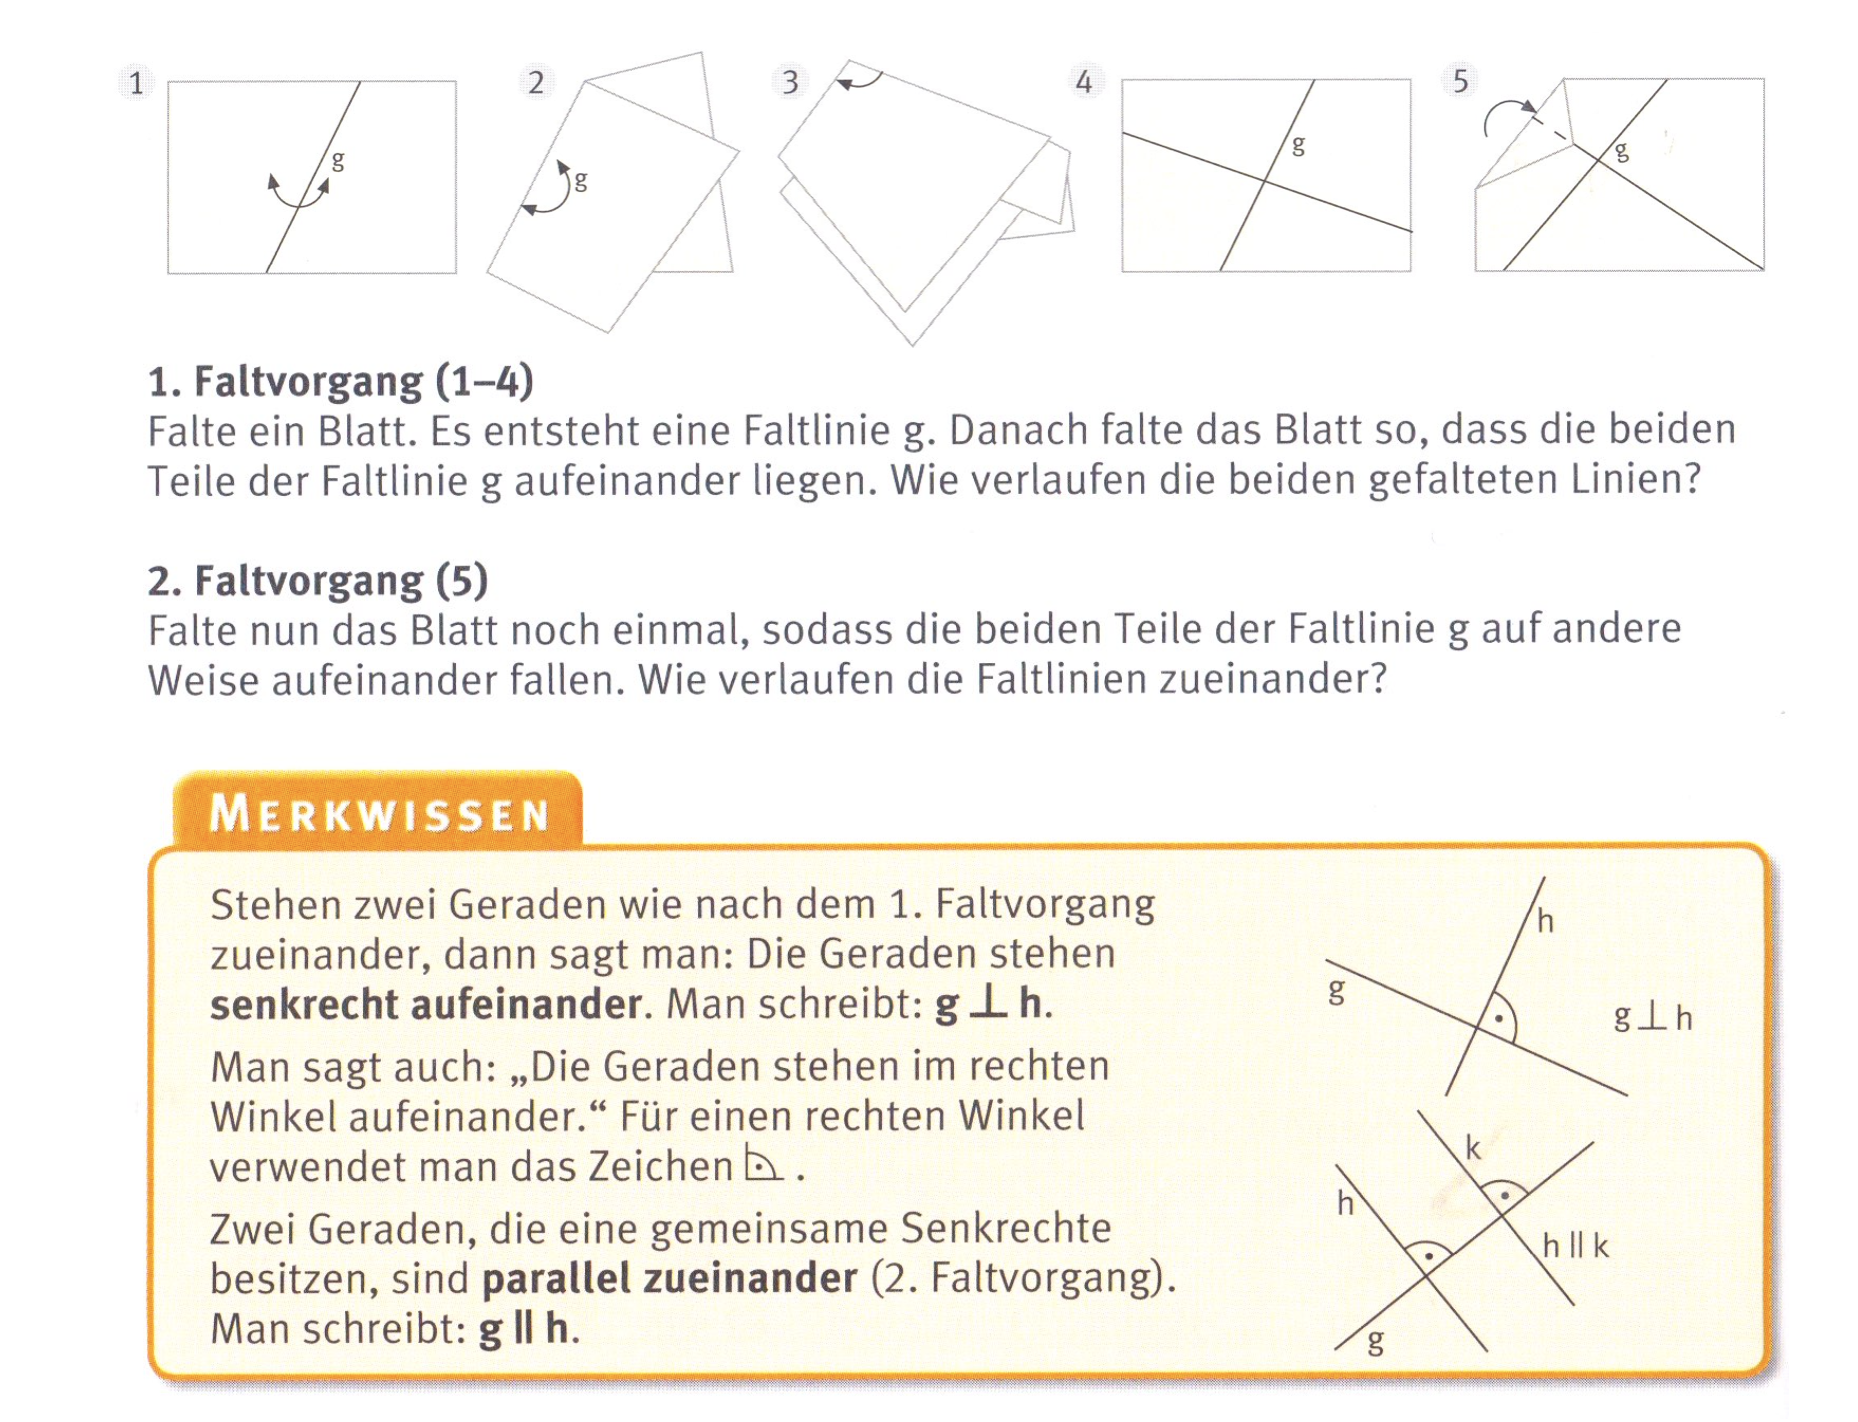
\includegraphics[width=1\linewidth]{pictures/6-SenkrechtDefinition} 

}

\caption{Definition zu den Begriffen \emph{senkrecht zueinander} und \emph{parallel zueinenader} (\protect\hyperlink{ref-Kleine2011}{Kleine, 2011, S. 78})}\label{fig:DefSenkrecht}
\end{figure}

\hypertarget{begriffe-handwerk-nachbereitung}{%
\section{Zum Nachbereiten}\label{begriffe-handwerk-nachbereitung}}

\begin{enumerate}
\def\labelenumi{\arabic{enumi}.}
\tightlist
\item
  Lesen Sie das Kapitel zur Begriffsbildung von \protect\hyperlink{ref-Weigand2015}{Weigand} (\protect\hyperlink{ref-Weigand2015}{2015}).
\item
  Wählen Sie einen Begriff und sammeln Sie geeignete Beispiele und Gegenbeispiele nach dem Variations- und Kontrastprinzip.
\end{enumerate}

Abbildung \ref{fig:BegriffeZusammenfassung} fasst die Inhalte dieses Kapitels noch einmal zusammen.

\begin{figure}

{\centering 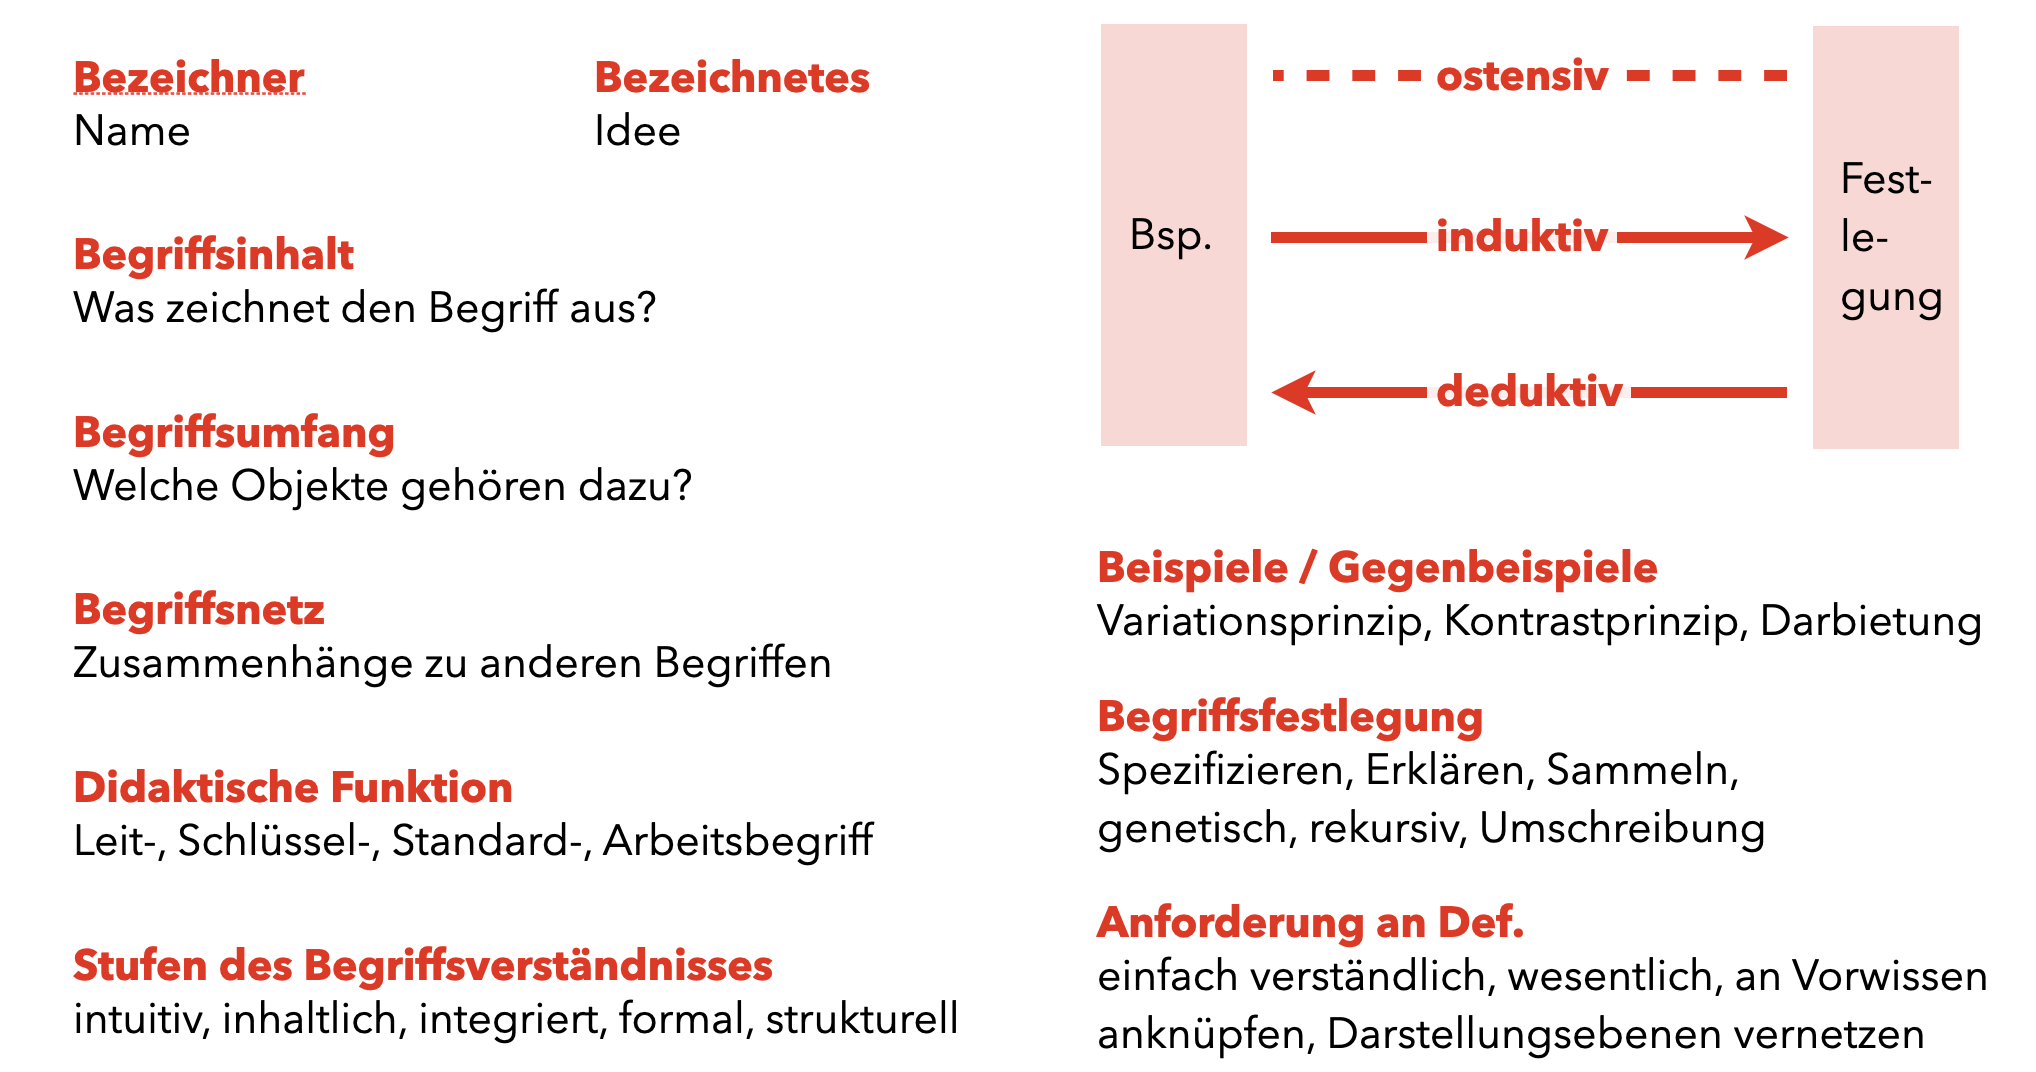
\includegraphics[width=0.9\linewidth]{pictures/6-Zusammenfassung} 

}

\caption{Zusammenfassung zur Begriffsbildung}\label{fig:BegriffeZusammenfassung}
\end{figure}

\hypertarget{bonus-operative-genese}{%
\section{Bonus: Operative Genese}\label{bonus-operative-genese}}

Eine weitere Möglichkeit der Begriffseinführung ist die \emph{Umwelterschließung im Geometrieunterricht durch operative Begriffsbildung} nach \protect\hyperlink{ref-Bender1978}{Bender} (\protect\hyperlink{ref-Bender1978}{1978}). Dabei geht man davon aus, dass sich die Begriffe der Mathematik an Phänomenen aus der Umwelt orientieren.

Orientierung heißt, dass reale Objekte dahingehend analysiert werden, welchen \textbf{Zweck} sie erfüllen. Betrachtet man zum Beispiel Ziegelsteine, erfüllen diese den Zweck, eine Mauer bauen zu können. Um dies zu ermöglichen, müssen die Steine eine bestimmte \textbf{Funktion} erfüllen, im konkreten Fall das Übereinanderstapeln handlicher Objekte zu einem i.~d.~R. rechtwinkligen Gesamtobjekt im Raum. Aus diesen Funktionen heraus kann nun das Objekt idealisiert werden, woraus sich Bedingungen ergeben, die es erfüllen muss. Der Ziegelstein muss also aus »ebenen, paarweise parallelen Seitenflächen und rechten Kantenwinkeln« bestehen (\protect\hyperlink{ref-Bender1978}{Bender, 1978, S. 36}), was zum \textbf{Begriff} des Quaders führt. Daraus abgeleitet kann nun wieder das \textbf{Realisat} hergestellt werden, also echte Quader.



\begin{figure}

{\centering 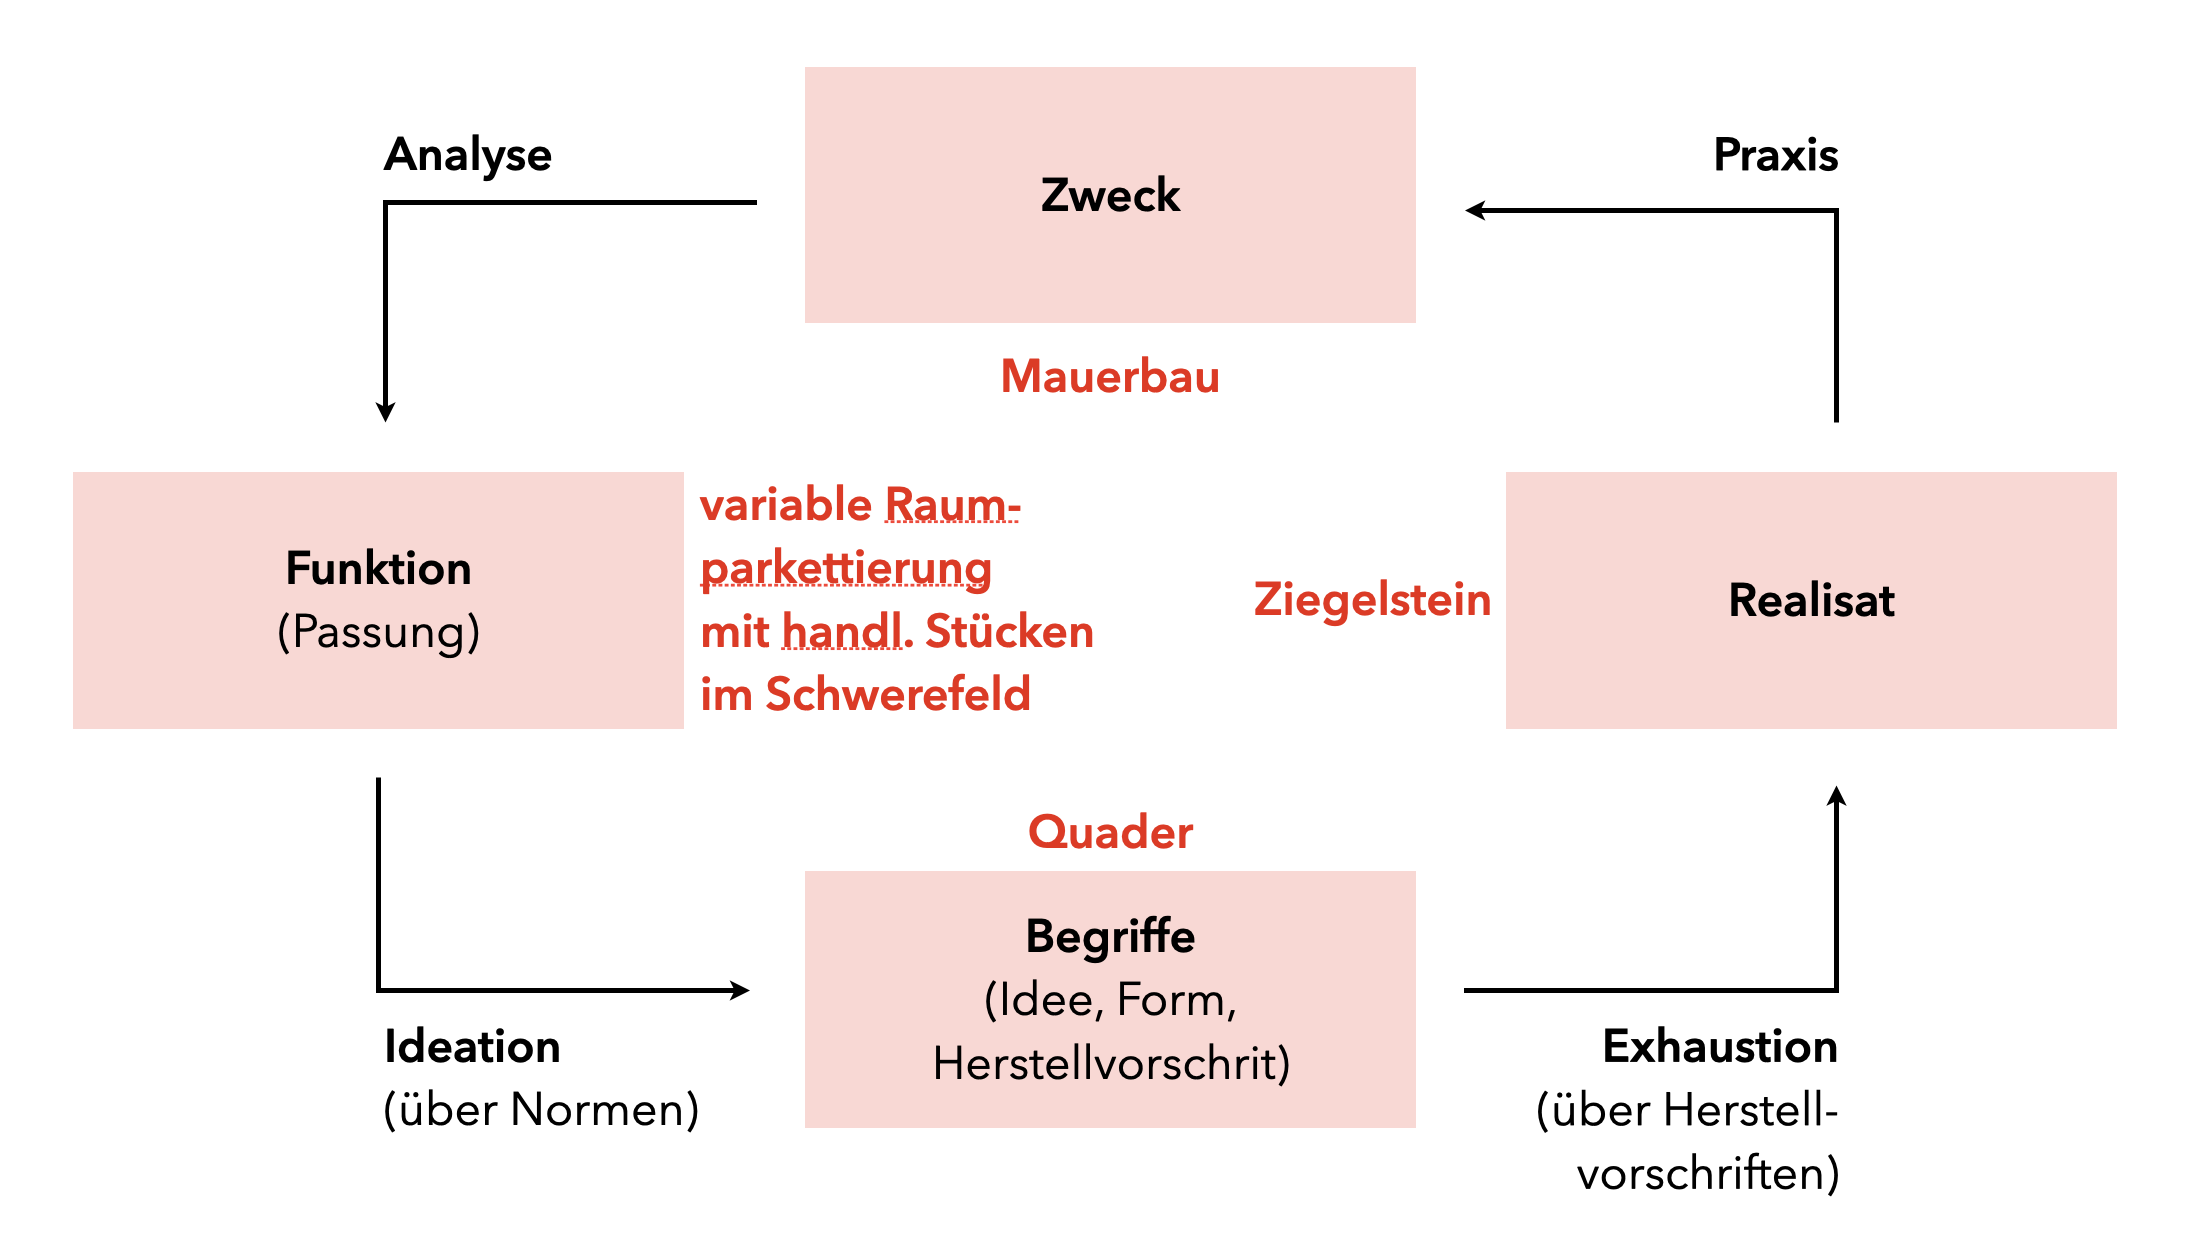
\includegraphics[width=1\linewidth]{pictures/6-operativ} 

}

\caption{Operative Genese in der Geometrie nach \protect\hyperlink{ref-Bender1978}{Bender} (\protect\hyperlink{ref-Bender1978}{1978, S. 35})}\label{fig:OperativeGenese}
\end{figure}

In dem Beispiel heißt die Orientierung an der Umwelt nicht, dass Quader das Ergebnis eines Abstraktionsprozesses sind (in dem Sinne, dass man echte Ziegelsteine nimmt, ansieht und feststellt, dass sie bestimmte Eigenschaften haben), sondern genau andersrum: Echte Quader sind die Ergebnisse, denen die mathematische Idee schon (über ihre Anwendung in der Umwelt) zugrunde liegt. Ggf. ist auch ein mehrmaliges Durchlaufen des Schemas notwendig, wobei der Bau von Modellen als Zwischenschritt zwischen Idee und Realisat dienen kann.

\hypertarget{lehr-lern-prozesse}{%
\chapter{Lehr-Lern-Prozesse}\label{lehr-lern-prozesse}}

\begin{quote}
\textbf{Lernziele}

\begin{itemize}
\tightlist
\item
  Sie kennen Grundideen der Tätigkeitstheorie.
\item
  Sie kennen die Lehrstrategie des Aufsteigens vom Abstrakten zum Konkreten und können diese mit der konkreten Ebene des Vier-Ebenen-Ansatzes und der Ausbildung von Grundvorstellungen in Bezug bringen.
\item
  Sie sind sich der Herausforderungen im Finden von Kontexten und Kernideen bewusst.
\end{itemize}

\textbf{Material}

\begin{itemize}
\tightlist
\item
  Folien zur Vorlesung zu Lehr-Lern-Prozessen (\href{files/Stoffdidaktik-WiSe2122-Kap7.pdf}{pdf}, \href{files/Stoffdidaktik-WiSe2122-Kap7.key}{Keynote})
\end{itemize}
\end{quote}

In diesem Kapitel sollen Grundideen der \emph{Tätigkeitstheorie} aufgegriffen und mit der konkreten Ebene des Vier-Ebenen-Ansatzes in Bezug gebracht werden. Ziel ist es, Lernprozesse (insbesondere zur Begriffsbildung) aus theoretischer Perspektive zu beschreiben und daraus Rückschlüsse auf die Gestaltung von Unterricht abzuleiten. Die Tätigkeitstheorie ist dabei nur \emph{eine} Möglichkeit, Lernen zu beschreiben -- und wird hier insbesondere aufgrund des entsprechenden Forschungsschwerpunktes an der Universität Potsdam gewählt.

\hypertarget{tuxe4tigkeitstheoretische-sicht}{%
\section{Tätigkeitstheoretische Sicht}\label{tuxe4tigkeitstheoretische-sicht}}

\hypertarget{grundannahmen}{%
\subsection{Grundannahmen}\label{grundannahmen}}

Eine Grundannahme der Tätigkeitstheorie ist das Verständnis, dass sich Individuen aktiv-handelnd mit ihrer Umwelt auseinandersetzen, die Umwelt dabei in der Interaktion mit der Gesellschaft verändern, und beide Prozesse wiederum psychisch im Individuum abgebildet werden. Dies widerspricht bspw. der \emph{behavioristischen} Annahme, dass man sich seiner Umwelt einfach nur anpasst, aber es ist auch nicht mit der \emph{konstruktivistischen} Annahme zu verwechseln, nach der Individuen ein Abbild der Umwelt kognitiv rekonstruieren. Die Tätigkeitstheorie kann eher als »(moderat) konstruktivistische{[}r{]}{[}..{]} Ansatz« bezeichnet werden (\protect\hyperlink{ref-Giest2016a}{Giest, 2016, S. 47}).

Weiterhin besteht die Annahme, dass Lernprozesse niemals direkt zwischen einem Individuum (dem \textbf{Subjekt}) und dem zu betrachtenden Lerngegenstand (dem \textbf{Objekt}) erfolgen, sondern dies stets über ein \textbf{vermittelndes Werkzeug} geschieht. Ein solches Werkzeug kann eine Geste sein, die Sprache (ein sogenanntes \emph{psychisches Werkzeug}), Abbildungen und Skizzen, aber eben auch \emph{echte} Werkzeuge wie Maschinen, Geräte und andere Hilfsmittel.

\begin{figure}

{\centering 
\includegraphics[width=0.75\linewidth]{pictures/7-SubjektObjekt} 

}

\caption{Werkzeuge als Vermittler in der Tätigkeitstheorie}\label{fig:SubjektObjekt}
\end{figure}

Durch die Nutzung eines geeigneten Werkzeugs ist das Subjekt damit also einerseits in der Lage, sein eigenes Wissen zu \emph{externalisieren}, d.~h. das Werkzeug zielgerichtet so einzusetzen, dass auf das Objekt eingewirkt werden kann. Andererseits kann das Werkzeug auch dabei helfen, Eigenschaften des Objekts zu \emph{internalisieren}, indem die Werkzeugnutzung dazu führt, dass das Subjekt Wissen über das Objekt aufbaut.

Für die Gestaltung von Mathematikunterricht ist nun von besonderem Interesse, welche Werkzeuge bei bestimmten Begriffen geeignet sind bzw. wie diese auszusehen haben, um den Begriffserwerb zu unterstützen. Die Tätigkeitstheorie ist noch deutlich komplexer als hier in wenigen Zeilen dargestellt. Eine übersichtliche Einführung bietet z.~B. \protect\hyperlink{ref-Giest2016a}{Giest} (\protect\hyperlink{ref-Giest2016a}{2016}), speziell für die Werkzeuggestaltung im Mathematikunterricht siehe auch \protect\hyperlink{ref-Etzold2021}{Etzold} (\protect\hyperlink{ref-Etzold2021}{2021}).

\hypertarget{gestaltung-von-lehr-lern-prozessen}{%
\subsection{Gestaltung von Lehr-Lern-Prozessen}\label{gestaltung-von-lehr-lern-prozessen}}

Nach einer ausführlicheren theoretischen Betrachtung schlägt \protect\hyperlink{ref-Lompscher1983a}{Lompscher} (\protect\hyperlink{ref-Lompscher1983a}{1983a, S. 77~f.}) für die Gestaltung von Lehr-Lern-Prozessen folgende Abfolge vor:

\begin{enumerate}
\def\labelenumi{\arabic{enumi}.}
\item
  Zunächst einmal sollte den Schülerinnen und Schülern eine Anforderungssituation in ihrer \textbf{Zone der nächsten Entwicklung} (ZdnE) präsentiert werden. Dies ist eine Problemsituation, Aufgabe oder Fragestellung, die die Schülerinnen und Schüler zwar mithilfe ihres bisherigen Wissens und Könnens verstehen und nachvollziehen können, zu ihrer Lösung sie jedoch noch nicht in der Lage sind. Damit soll eine Motivation geschaffen werden, sich mit der Thematik tiefer auseinanderzusetzen. Es ist durchaus möglich, an dieser Stelle auch schon erste Lösungsversuche zu unternehmen. Daran ist besonders gut zu erkennen, »was wir nicht wissen bzw. können, um die Anforderung zu bewältigen« (\protect\hyperlink{ref-Lompscher1996}{Lompscher, 1996, S. 4}).
\item
  Anschließend werden gemeinsam mit der Lehrkraft \textbf{Lernziele} herausgearbeitet, die den weiteren Verlauf des Lernens strukturieren sollen. Wichtig ist hier eine Unterscheidung zu \emph{Lehrzielen}, die die Sicht der Lehrkraft widerspiegeln. \emph{Lernziele} dagegen sind die Ziele aus Sicht der Schülerinnen und Schüler, auf die sich im individuellen Lernprozess auch bezogen werden können muss. Es bietet sich daher auch eine explizite Formulierung der Lernziele an.
\item
  Nun wird durch den \textbf{Aufbau von Lernhandlungen} auf den Lerngegenstand eingewirkt. Lernhandlungen sind nach \protect\hyperlink{ref-Lompscher1983}{Lompscher} (\protect\hyperlink{ref-Lompscher1983}{1983b, S. 46}) »relativ geschlossene und abgrenzbare, zeitlich und logisch strukturierte Abschnitte im Verlauf der Lerntätigkeit, die ein konkretes Lernziel realisieren, durch bestimmte Lernmotive angetrieben werden und entsprechend den konkreten Lernbedingungen durch den Einsatz äußerer und verinnerlichter Lernmittel in einer jeweils spezifischen Folge von Teilhandlungen vollzogen werden.« Konkreter lässt sich dies auch nicht wirklich beschreiben -- je nach Lerngegenstand sind von der Lehrkraft geeignete Lernhandlungen zu identifizieren. Entscheidend ist, dass die Lernhandlungen das Wesen des Lerngegenstands repräsentieren, damit über sie das Wissen aufgebaut werden kann.
\item
  Um nun den Lerngegenstand (also das \emph{Objekt}) psychisch (im \emph{Subjekt}) abbilden zu können, ist eine \textbf{Verinnerlichung der Lernhandlungen} nötig. Nach Gal'perin bietet sich hierfür eine \emph{etappenweise Verinnerlichung} an (vgl. \protect\hyperlink{ref-Lompscher1983a}{Lompscher, 1983a, S. 66~f.}):

  \begin{itemize}
  \item
    \textbf{Etappe der materiellen bzw. materialisierten Handlung}

    Die Handlungen werden mit dem konkreten Material bzw. Repräsentationen durchgeführt.
  \item
    \textbf{Etappe der sprachlichen Handlung}

    Die Handlungen werden nicht mehr direkt durchgeführt, aber durch äußeres (oder inneres) Sprechen beschrieben. Dabei wird i.~d.~R. Bezug auf die vorherigen Handlungen genommen.
  \item
    \textbf{Etappe der geistigen Handlung}

    Die Handlungen werden nun rein kognitiv durchgeführt und bedürfen weder des Materials noch der Sprache.
  \end{itemize}
\item
  Darauf aufbauend ist nun das \textbf{Lösen von Aufgaben} möglich, die zu einer weiteren Verankerung des neu erworbenen Wissens führen sollen.
\end{enumerate}

Insbesondere für die Bildung von Begriffen bietet sich für den Aufbau von Lernhandlungen und ihre Verinnerlichung das im folgenden Abschnitt beschriebene Vorgehen an:

\hypertarget{aufsteigen-vom-abstrakten-zum-konkreten}{%
\subsection{Aufsteigen vom Abstrakten zum Konkreten}\label{aufsteigen-vom-abstrakten-zum-konkreten}}

Die sogenannte Lehrstrategie des \textbf{Aufsteigens vom Abstrakten zum Konkreten} (siehe Abbildung \ref{fig:Aufsteigen}) kann als Abwandlung einer Mischung zwischen induktivem und deduktivem Vorgehen angesehen werden.



\begin{figure}

{\centering 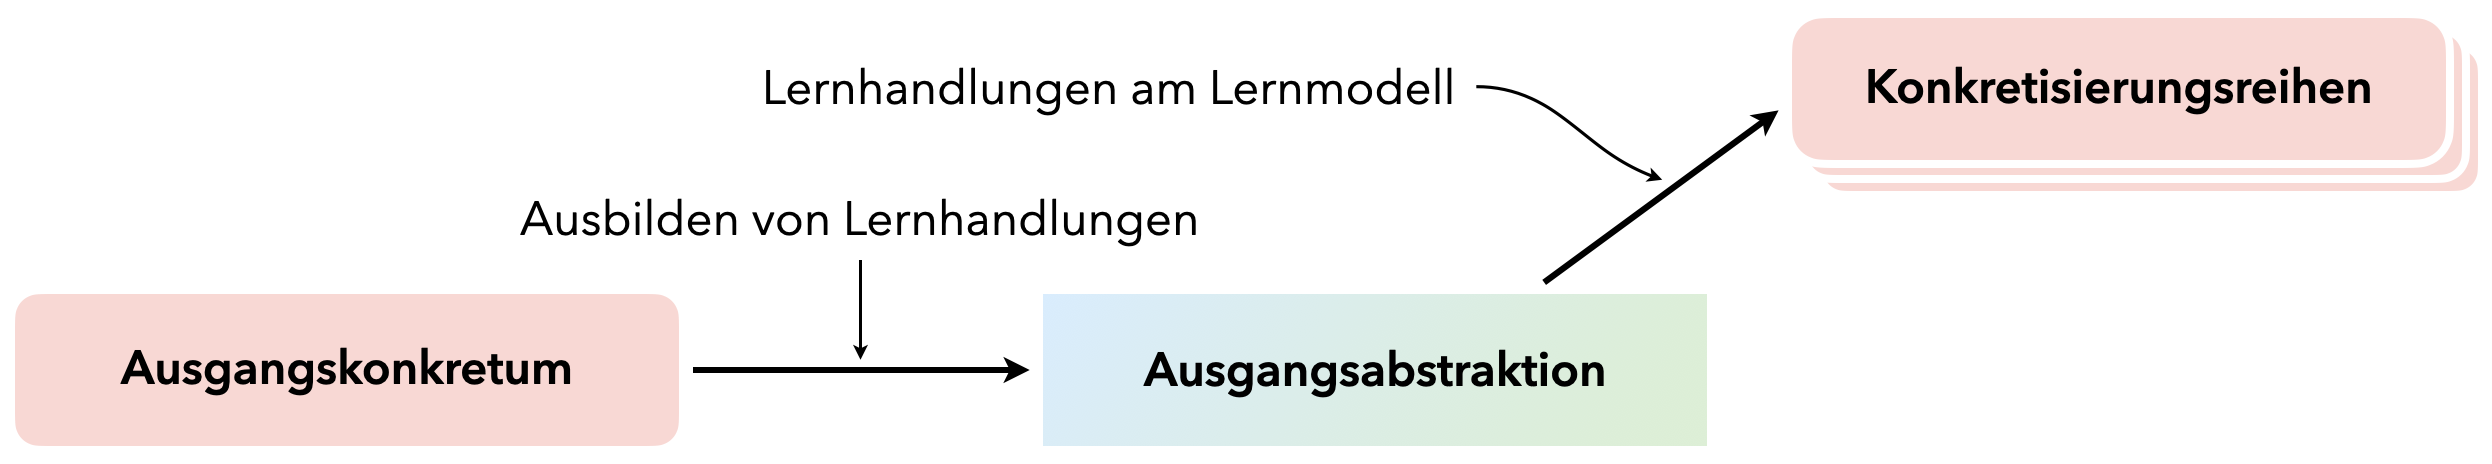
\includegraphics[width=1\linewidth]{pictures/7-AK} 

}

\caption{Aufsteigen vom Abstrakten zum Konkreten (vgl. \protect\hyperlink{ref-Etzold2021}{Etzold, 2021, S. 83})}\label{fig:Aufsteigen}
\end{figure}

Für die Einführung eines mathematischen Begriffs wird ein konkretes Ausgangsbeispiel gewählt, an dem das Wesen des Begriffs besonders gut deutlich wird. An diesem \textbf{Ausgangskonkretum} werden Lernhandlungen erarbeitet, die sich zwar am Beispiel orientieren, aber verallgemeinern lassen, sodass sie dem Begriffsaufbau dienlich sind.

Im Anschluss wird, mit Unterstützung der Lehrkraft, das Wesen des Begriffs herausgearbeitet und in Form einer \textbf{Ausgangsabstraktion} formuliert. Dieses Vorgehen ist vergleichbar mit dem induktiven Begriffserwerb, allerdings wird nicht aus einer Vielzahl von Beispielen eine gemeinsame Eigenschaft eliminiert, sondern am charakteristischen Beispiel wird die Eigenschaft durch eine \emph{wissende Person} (Lehrkraft) in Bezug auf die Handlungserfahrungen der Schülerinnen und Schüler dargestellt. Dieser Prozess wird unterstützt mithilfe von \textbf{Lernmodellen} -- als »sinnliche Stützen geistigen Handelns« (\protect\hyperlink{ref-Giest2006}{Giest \& Lompscher, 2006, S. 225}). Dies können Zeichnungen, strukturierte Darstellungen, digitale Anwendungen usw. sein, die das Wesen des Begriffs beeinhalten und erlebbar machen, wie man zu diesem Wesen gelangen kann.

Der dritte Schritt, das eigentliche \emph{Aufsteigen vom Abstrakten zum Konkreten}, ist nun das Abarbeiten von \textbf{Konkretisierungsreihen}. Hierzu werden weitere Beispiele für den Begriff betrachtet, auf die das Ausgangsabstraktum angewandt wird. Das Lernmodell dient dabei als Mittler und die Lernhandlungen werden in verallgemeinerter und ggf. auch modifizierter Form angewandt. Erst auf diese Weise ist ein echtes \emph{Durchdringen} des Begriffs möglich. Dieses Vorgehen ist mit dem deduktiven Vorgehen vergleichbar, allerdings nicht im dem Sinne, dass aus einer Definition heraus die Beispiele generiert werden. Vielmehr wird auf gegebene Beispiele die Definition angewandt, ausgeschärft und damit der Begriff immer besser verstanden.

Bereits in Abschnitt \ref{konkrete-ebene} wurde das Beispiel des Begriffs \emph{Winkelfeld} kurz dargestellt. Das \emph{Ausgangskonkretum} waren dort Sichtfelder von Tieren, da an diesen die Feld-Eigenschaft eines Winkelfeldes in besonderer Weise deutlich wird und auch die weiteren Bestandteile des Winkelfeldes (Scheitelpunkt, Schenkel) eine bedeutsame reale Entsprechung (Kopf des Tieres, Begrenzung des Sichtfeldes) haben. Eine mögliche \emph{Lernhandlung} war es, das Schaf so zu bewegen, dass es die gesamte Zeit über von der Kuh \emph{gerade noch so} gesehen wird (siehe Abbildung \ref{fig:HandlungSchaf}).



\begin{figure}

{\centering 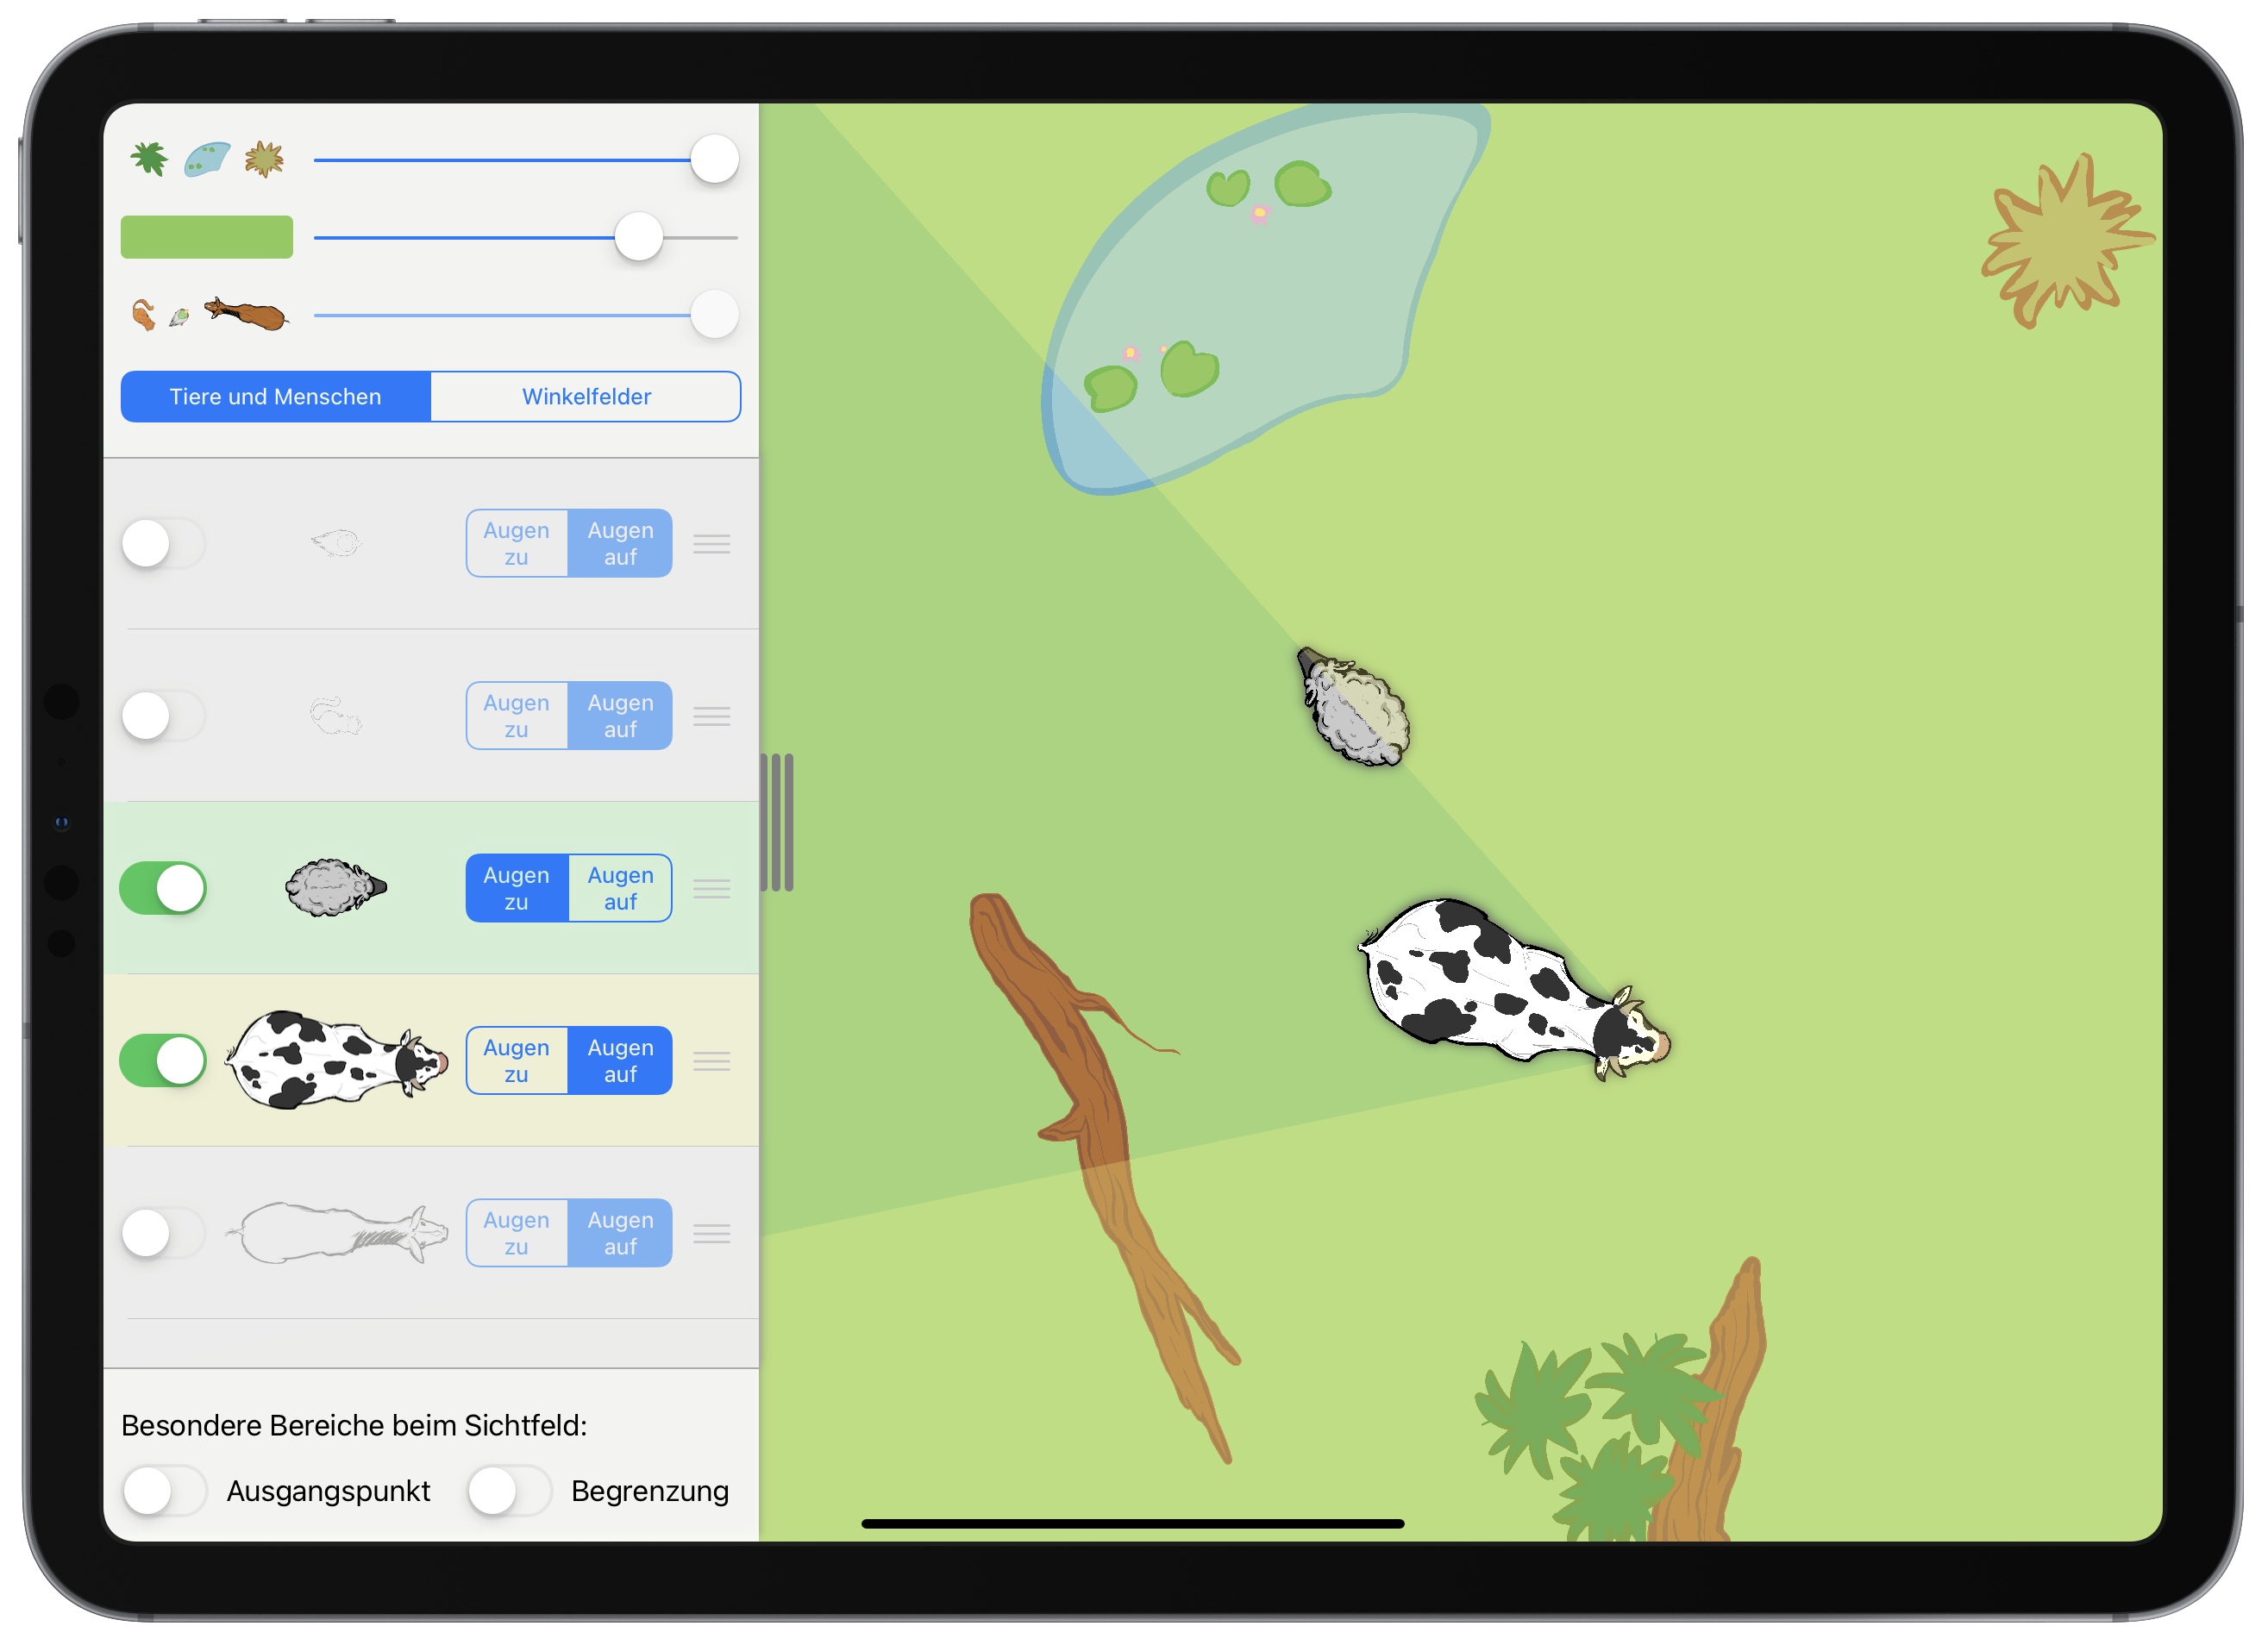
\includegraphics[width=0.5\linewidth]{pictures/2-Winkelfarm} 

}

\caption{Lernhandlung in der App \emph{Winkel-Farm} (\protect\hyperlink{ref-Etzold:2019}{Etzold, 2019a})}\label{fig:HandlungSchaf}
\end{figure}

Dabei erfolgt die Bewegung geradlinig, in Richtung des Kopfes der Kuh begrenzt und in die andere Richtung unbegrenzt. In verallgemeinerter Form wird damit die Strahl-Eigenschaft des Schenkels charakterisiert. Die App mit der Möglichkeit, die Bestandteile des Winkelfeldes ein- und ausblenden zu lassen sowie vom \emph{Tiermodus} in den \emph{Winkelfeldmodus} zu wechseln, stellt dabei das \emph{Lernmodell} dar. \emph{Konkretisierungreihen} sind an diesem Beispiel noch nicht erfolgt.

\hypertarget{bezug-zum-vier-ebenen-ansatz}{%
\section{Bezug zum Vier-Ebenen-Ansatz}\label{bezug-zum-vier-ebenen-ansatz}}

Das oben beschriebene Vorgehen bietet die Möglichkeit, die Fragen der \textcolor{concreteColor}{konkreten Ebene} des \protect\hyperlink{tab:fragen-ebenen}{Vier-Ebenen-Ansatzes} anzugehen. Dies wird insbesondere deutlich, wenn man den Aufbau des Schulbuchs \emph{Mathewerkstatt} (\protect\hyperlink{ref-Barzel2012}{Barzel et al., 2012c})\footnote{Zur besseren Lesbarkeit wird auf die Zitation der \emph{Mathewerkstatt} im restlichen Kapitel verzichtet.} betrachtet, das als Basis die Fragestellungen des Vier-Ebenen-Ansatzes hat. So lassen sich dort vom Vorgehen her Elemente wiederfinden, die mit den tätigkeitstheoretischen Grundlagen und der daraus abgeleiteten Gestaltung von Lehr-Lern-Prozessen vereinbar sind. Der entsprechende Zusammenhang wird auch von den Autorinnen und Autoren der \emph{Mathewerkstatt} selbst implizit hergestellt, indem die im Schulbuch auftretenden \emph{Kernprozesse} mit den von Bruder als Vertreterin der Tätigkeitstheorie formulierten \emph{Unterrichtssituationen} in Beziehung gesetzt werden (siehe \protect\hyperlink{ref-Prediger2014}{Prediger et al., 2014}).

\hypertarget{kontexte-kernideen-kernfragen}{%
\subsection{Kontexte, Kernideen, Kernfragen}\label{kontexte-kernideen-kernfragen}}

Der von \protect\hyperlink{ref-Hussmann:2016}{Hußmann \& Prediger} (\protect\hyperlink{ref-Hussmann:2016}{2016}) geforderte \textbf{Kontext}, der geeignet sein soll, sich dem Lerngegenstand zu nähern, kann über die \textbf{Zone der nächsten Entwicklung} motiviert werden und sich im \textbf{Ausgangskonkretum} widerspiegeln. In der \emph{Mathewerkstatt} ist dies die \emph{Anküpfung} auf der Einstiegsseite (am Beispiel des \protect\hyperlink{erstes-intermezzo-flaecheninhalt}{Ersten Intermezzos} die Situation der Tiergehe, siehe Abbildung \ref{fig:Tiergehege}). \protect\hyperlink{ref-Leuders2011}{Leuders et al.} (\protect\hyperlink{ref-Leuders2011}{2011, S. 4}, Hervorhebungen im Original) formulieren:

»Ein \emph{sinnstiftender Kontext} ist ein Ausschnitt einer inner- oder außermathematischen Welt, der folgende Anforderungen möglichst gut erfüllt:

\begin{itemize}
\tightlist
\item
  Er ist anschlussfähig an die Erfahrungen, Interessen und die Denk- und Handlungsmuster der Lernenden \emph{(Lebensweltbezug)}.
\item
  Er ermöglicht es, authentische Fragen zu bearbeiten und dabei auch etwas über den Kontext zu lernen \emph{(Kontextauthentizität)}.
\item
  Er ist problemhaltig und offen genug, um Lernende zum reichhaltigen Fragen und Erkunden anzuregen \emph{(Reichhaltigkeit)}.«
\end{itemize}

Daran anknüpfend werden \textbf{Kernideen} sichtbar gemacht, die in Form von \textbf{Kernfragen} formuliert und beantwortet werden (am Beispiel des \protect\hyperlink{erstes-intermezzo-flaecheninhalt}{Ersten Intermezzos}: \emph{Wie kann ich die Größe von Flächen vergleichen?}, \emph{Wie kann ich die Größe einer Fläche geschickt bestimmen?}). Deren Ziel ist es, sich aus Perspektive der Schülerinnen und Schüler dem Wesen des Begriffs nähern zu können. In der Lehrstrategie des Aufsteigens vom Abstrakten zum Konkreten erfolgt dies sowohl bei der Ausübung der \textbf{Lernhandlung am Ausgangskonkretum}, als auch in der Verallgemeinerung der Lernhandlungen beim \textbf{Entwickeln der Ausgangsabstraktion} sowie in vertiefter Art und Weise beim \textbf{Abarbeiten der Konkretisierungsreihen}. Diese beiderseitige Entwicklung wird auch bei \protect\hyperlink{ref-Leuders2011}{Leuders et al.} (\protect\hyperlink{ref-Leuders2011}{2011, S. 8}, Hervorhebungen im Original fett oder fettkursiv, hier kursiv) sichtbar:

»Eine \emph{Kernidee} umfasst in \emph{Vorschauperspektive} Fragen, die die Lernenden stellen können und berücksichtigt so die subjektbezogene Dimension der Sinnstiftung. Die Kernidee in Frageform schließt an individuelle Vorerfahrungen, Zielperspektiven, Denk- und Handlungsmuster der Lernenden an und initiiert die Auseinandersetzung mit dem mathematischen Gegenstand in den Worten von Schülerinnen und Schülern{[}. \ldots{]}

Die zu einer Kernidee gehörenden Fragen fokussieren in genetischer Perspektive konkrete zentrale Probleme, die letztlich zur Entwicklung der ›Rückschauantworten‹ der Kernidee führen.

Eine \emph{Kernidee} beschreibt in der \emph{Rückschauperspektive} den ideenbezogenen Kern einer längeren Lernepisode{[}. \ldots{]}

Zur Kernidee gehört also die ›Rückschauantwort‹, in der eine allgemeine Problemstellung und die zu ihrer Bewältigung notwendigen mathematischen Konzepte benannt werden. Damit wird deutlich, dass eine Kernidee die Zwecke der Mathematisierungsprozesse und damit den Sinn der mathematischen Konzepte miterfasst.«

In der \emph{Mathewerkstatt} werden über die Prozesse des \emph{Erkundens} und \emph{Ordnens} diese Vor- und Rückschauperspektive realisiert und in den \emph{Vertiefungen} -- wie es das Wort schon sagt -- vertieft.

Abbildung \ref{fig:AKMathewerkstatt} zeigt noch einmal die Phasen in der \emph{Mathewerkstatt} (vgl. auch \protect\hyperlink{ref-Prediger2014}{Prediger et al., 2014}) mit einer möglichen Anknüpfung an die Lehrstrategie des Aufsteigens vom Abstrakten zum Konkreten.



\begin{figure}

{\centering 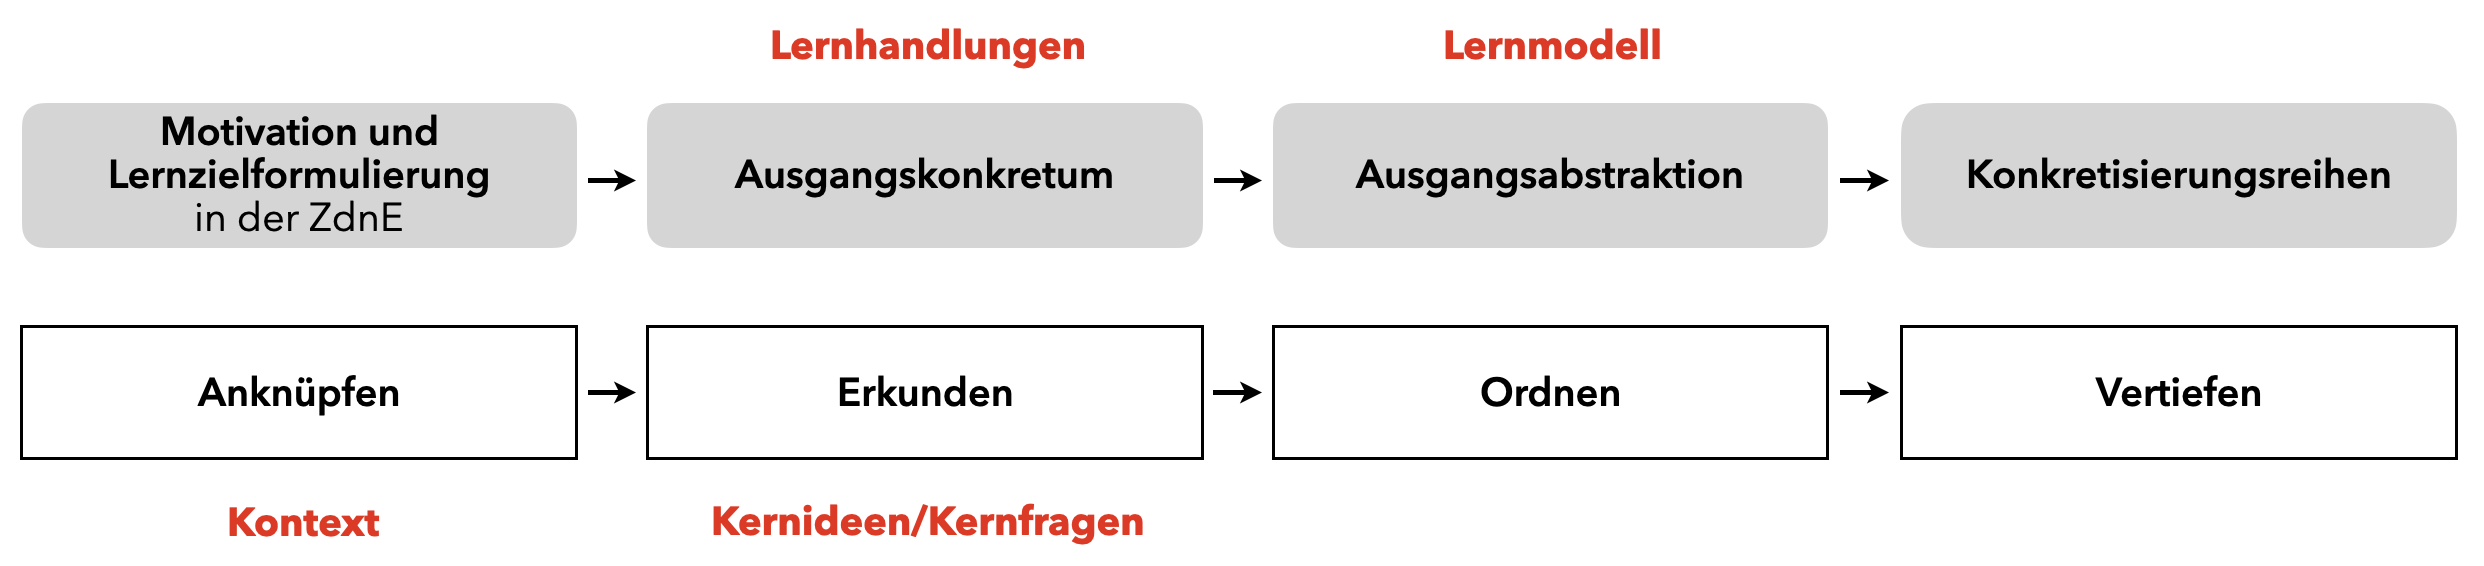
\includegraphics[width=1\linewidth]{pictures/7-Vergleich} 

}

\caption{Gegenüberstellung des Aufsteigens vom Abstrakten zum Konkreten mit dem Vorgehen in der \emph{Mathewerkstatt}}\label{fig:AKMathewerkstatt}
\end{figure}

\hypertarget{aufbau-von-grundvorstellungen}{%
\subsection{Aufbau von Grundvorstellungen}\label{aufbau-von-grundvorstellungen}}

Gemäß der Grundvorstellungsidee (siehe Def. \ref{def:Grundvorstellungen}) sollen Grundvorstellungen einen \emph{Handlungsbezug} aufweisen, operationsfähige \emph{Repräsentationen} beinhalten und eine \emph{Anwendung in der Realität} ermöglichen.

Mit den \textbf{Lernhandlungen} am Ausgangskonkretumg und den Konkretisierungsreihen ist der \textbf{Handlungsbezug} herstellbar, außerdem kann darüber die \textbf{Anwendung in der Realität} sichtbar gemacht werden -- sowohl beschreibend (von der Mathematik zur Realität) als auch modellierend (von der Realität zur Mathematik).

Das \textbf{Lernmodell} selbst kann als \textbf{Repräsentation} dienen, anhand dessen mit dem Begriff operiert wird. Dies ist ja auch eine Eigenschaft des Lernmodells: Sie sind eine »abstrakte Struktur des Gegenstands zusammen mit dem prinzipiellen Weg {[}..{]}, der zur Aufdeckung der Struktur geführt hat« (\protect\hyperlink{ref-Lompscher1996}{Lompscher, 1996, S. 6}).

Auch das \textbf{Verinnerlichen der Lernhandlungen} kann dem Aufbau von Grundvorstellungen dienen. So stellen bspw. \protect\hyperlink{ref-Wartha2011}{Wartha \& Schulz} (\protect\hyperlink{ref-Wartha2011}{2011, S. 11}) ein Vier-Phasen-Modell vor, dass stark an die etappenweise Verinnerlichung von Lernhandlungen nach Gal'perin erinnert.



\begin{figure}

{\centering 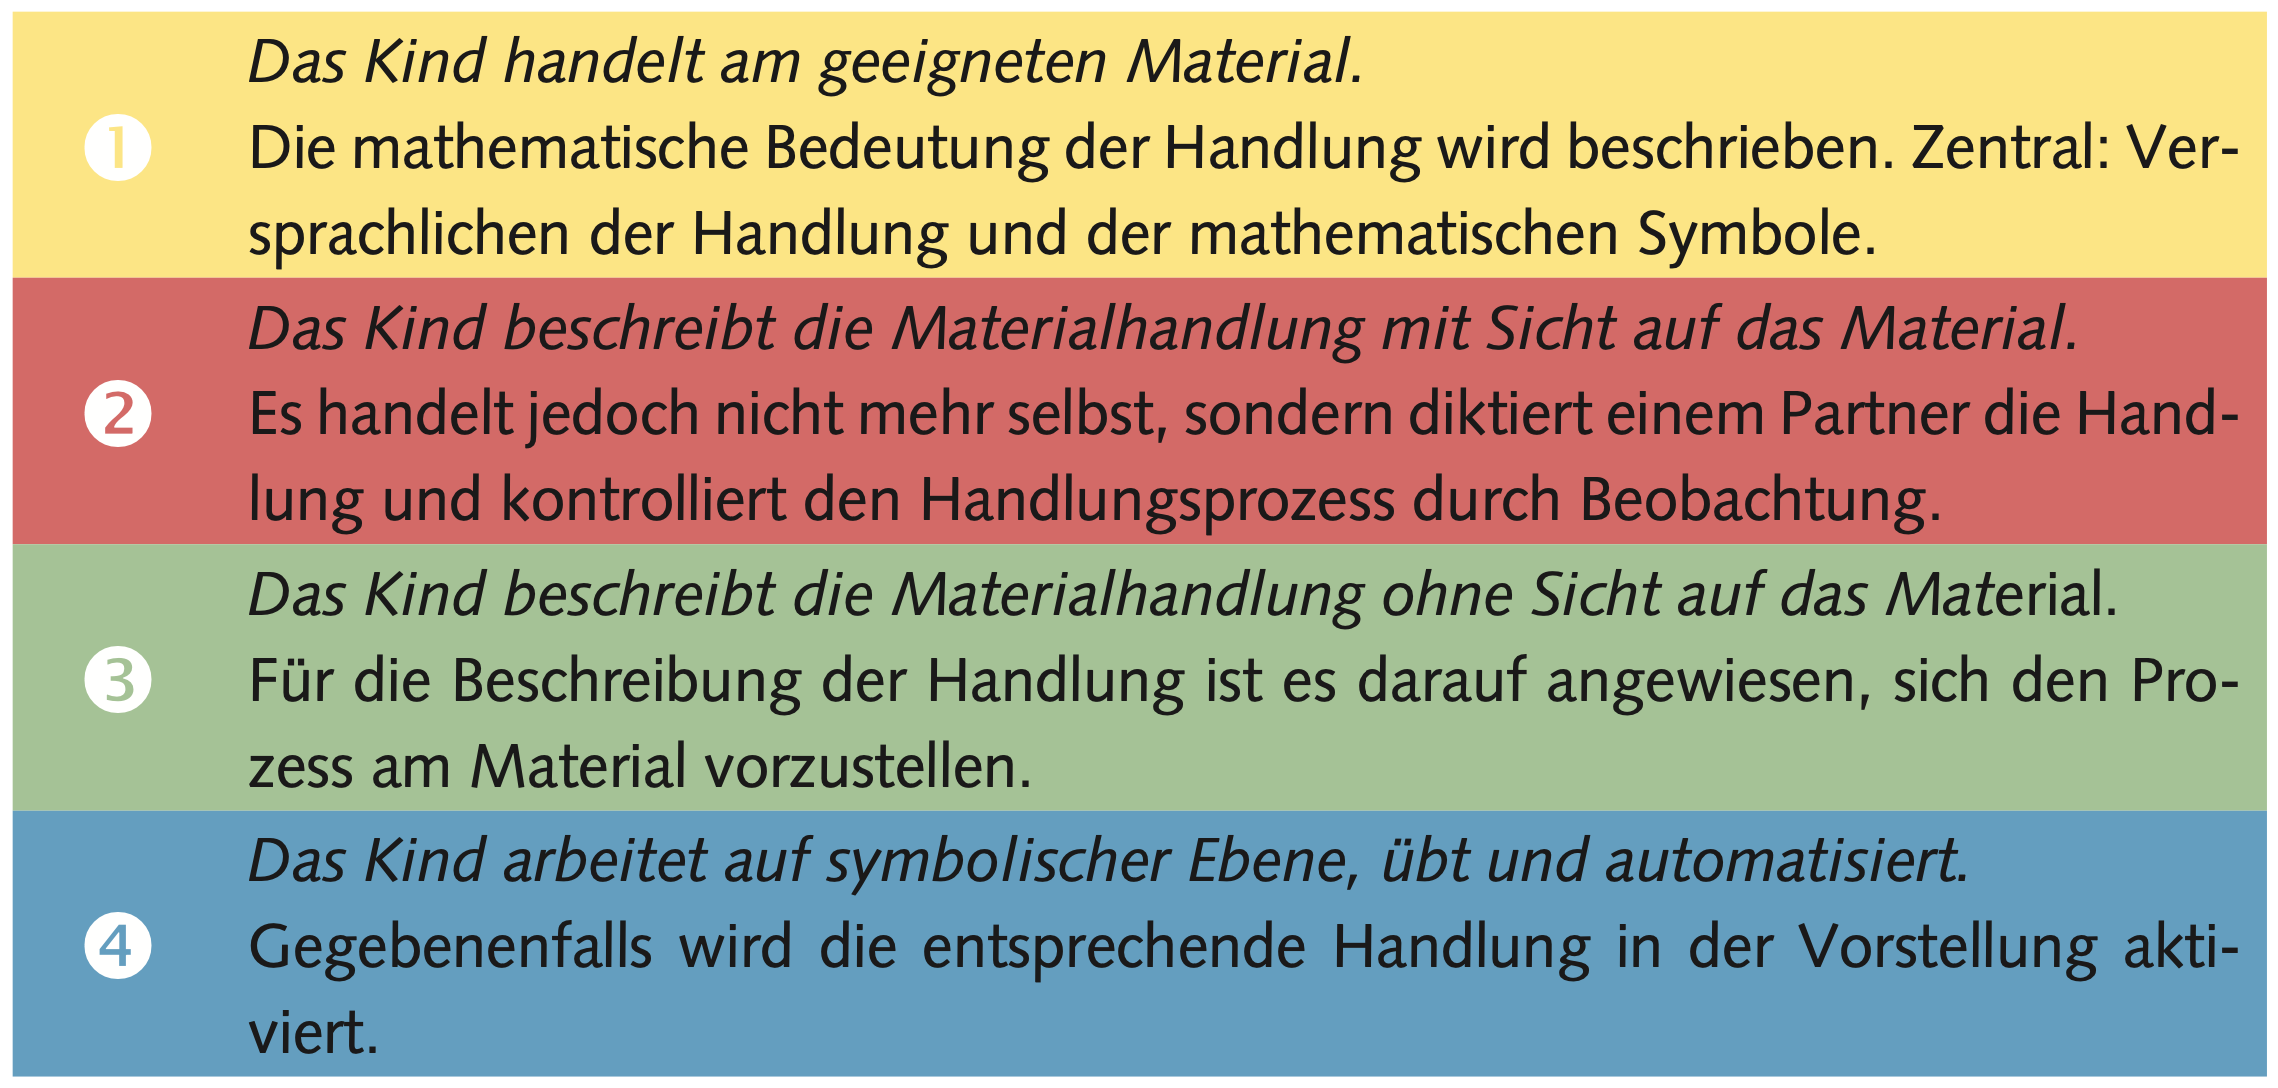
\includegraphics[width=0.9\linewidth]{pictures/7-GVverinnerlichen} 

}

\caption{Aufbau von Grundvorstellungen nach \protect\hyperlink{ref-Wartha2011}{Wartha \& Schulz} (\protect\hyperlink{ref-Wartha2011}{2011, S. 11})}\label{fig:GVVerinnerlichen}
\end{figure}

Für eine ausführlichere Darstellung zu den Zusammenhängen aus der Lehrstrategie des Aufsteigens vom Abstrakten zum Konkreten und der Grundvorstellungsidee siehe auch \protect\hyperlink{ref-Etzold2021}{Etzold} (\protect\hyperlink{ref-Etzold2021}{2021, S. 71~ff.}).

\hypertarget{begriffe-lerntheoretisch-nachbereitung}{%
\section{Zum Nachbereiten}\label{begriffe-lerntheoretisch-nachbereitung}}

\begin{enumerate}
\def\labelenumi{\arabic{enumi}.}
\item
  Lesen Sie den Beitrag von \protect\hyperlink{ref-Lompscher1996}{Lompscher} (\protect\hyperlink{ref-Lompscher1996}{1996}) zum Aufsteigen vom Abstrakten zum Konkreten.
\item
  Wählen Sie einen mathematischen Begriff und überlegen Sie sich, wie ein geeignetes Lernmodell für diesen Begriff aussehen kann. Sie können dabei auch spekulieren, was dieses Lernmodell können müsste (z.~B. wenn es digital umgesetzt werden könnte).
\end{enumerate}

\hypertarget{zweites-intermezzo-wurzel}{%
\chapter{Zweites Intermezzo: Wurzel}\label{zweites-intermezzo-wurzel}}

\begin{quote}
\textbf{Lernziele}

\begin{itemize}
\tightlist
\item
  Sie vertiefen Ihr Verständnis über den Vier-Ebenen-Ansatz, insbesondere zu Begriffsbildungsprozessen auf der konkreten Ebene.
\item
  Sie gewinnen einen Einblick in die Tätigkeitstheorie-basierte Gestaltung von Lernprozessen am Beispiel des Wurzelbegriffs.
\end{itemize}
\end{quote}

Am Beispiel des Begriffs \emph{Wurzel} sollen die in den letzten beiden Kapiteln dargestellten Inhalte auf der \textcolor{concreteColor}{konkreten} Ebene verdeutlicht werden. Um die Überlegungen zur Begriffsbildung anstellen zu können, wäre vorher eine Analyse auf der \textcolor{formalColor}{formalen} und \textcolor{semanticColor}{semantischen} Ebene notwendig. Darauf wird hier der Übersichtlichkeit halber verzichtet -- entsprechende Gedanken fließen implizit ein.

\hypertarget{wurzel-begriffsverstuxe4ndnis}{%
\section{Wurzel-Begriffsverständnis}\label{wurzel-begriffsverstuxe4ndnis}}

Als \textbf{Begriffsinhalt} des Wurzelbegriffs ist zunächst festzuhalten, dass die Wurzel bzw. das Wurzelziehen die Umkehrung des Quadrierens im Bereich der nichtnegativen Zahlen ist. Diese Nichtnegativität ist übrigens im Unterricht besonders herauszuarbeiten. Während \((-3)^2 = 9\) und \(3^2= 9\) ist, also die Gleichung \(x^2 = 9\) zwei Lösungen in den reellen Zahlen hat, ist \(\sqrt{9} = 3\) eindeutig festgelegt. Man kann also nicht pauschal von der Wurzel als die Umkehrung des Quadrates sprechen.\footnote{Dies wird bei höheren Exponenten sogar noch bedeutsamer: Dort ist \((-3)^3 = -27\). Die Gleichung \(x^3 = -27\) ist im Reellen sogar eindeutig lösbar (im Komplexen dagegen hat sie drei Lösungen), aber \(\sqrt[3]{-27}\) ist nicht definiert. Gerade, weil einige Taschenrechner fälschlicherweise die dritte Wurzel aus \(-27\) mit \(-3\) angeben, muss auf eine derartige Gefahr eingegangen werden, wenn Wurzeln höherer Exponenten behandelt werden. Dies zeigt einmal mehr, dass Sie als Lehrkraft über den aktuellen Unterrichtsstoff (z.~B. Quadratwurzeln) hinausdenken müssen (z.~B. Kubikwurzeln), um Rückschlüsse ziehen zu können, welche inhaltlichen Besonderheiten zu betonen sind.} Weiterhin zum Begriffsinhalt gehört die Eigenschaft, dass Wurzeln nicht immer rational sein müssen, auch wenn die Zahl, aus der die Wurzel gezogen wird, rational ist (z.~B. bei \(\sqrt{2}\)). Der Wert einer Wurzel lässt sich jedoch mittels rationaler Zahlen annähern\footnote{Die fachmathematische Grundlage hierfür ist, dass Cauchy-Folgen in den reellen Zahlen immer konvergieren und sich die nichtnegative Lösung der Gleichung \(x^2 = a\) mit \(a\geq 0\) über eine rationale Cauchy-Folge nähern lässt -- konkret mit dem \emph{Heron-Verfahren}.}. Das Vorgehen zum Finden einer Annäherung kann durchaus auch als Bestandteil des Begriffsinhalts aufgefasst werden.

Der \textbf{Begriffsumfang} der Wurzel sind demnach alle nichtnegativen reellen Zahlen, da für jede (rationale oder reelle) Zahl \(a\geq 0\) eine reelle Zahl \(x\geq 0\) gefunden werden kann, für die \(x^2 = a\) gilt. Dieser Begriffsumfang kann sich jedoch erst schrittweise entwickeln, da mit der Einführung des Wurzelbegriffs in der Regel noch nicht die reellen Zahlen bekannt sind. Die Menge aller Wurzeln rationaler Zahlen besteht zwar aus nichtnegativen reellen Zahlen -- aber noch nicht aus allen (denn z.~B. \(\sqrt{\pi}\) existiert ja auch). Ein vollständiger Begriffsumfang des Wurzelbegriffs ist also erst dann ausgeprägt, wenn die reellen Zahlen eingeführt wurden.

Damit werden auch schon Zusammenhänge des \textbf{Begriffsnetzes} sichtbar. Eng verbunden ist der Wurzelbegriff mit dem des \emph{Quadrates} (sowohl algebraisch als auch geometrisch) und den \emph{Reellen Zahlen} (als \emph{Lückenfüller} der rationalen Achse). Auch das \emph{Wurzelziehen} bzw. \emph{Radizieren}\footnote{Hier lohnt es sich übrigens, auf die Wortherkunft einzugehen und zu begründen, warum Radieschen als solche bezeichnet werden.} als verwandte Arbeitsbegriffe gehören zum engen Begriffsnetz. Bei der Betrachtung der Gleichung \(x^2 = a\) sind auch \emph{Basis} und \emph{Exponent} sowie der \emph{Radikant}, v.~a. in der Schreibweise \(\sqrt{a} = x\), Bestandteile des Begriffsnetzes. Der \emph{Wurzelexponent} wird dann v.~a. bei höheren Exponenten von Bedeutung, wenn er in der Schreibweise \(\sqrt[n]{a}\) auftritt. Ob die \emph{Intervallschachtelung} als Fachbegriff im Zusammenhang mit dem Wurzelziehen auftauchen muss, sollte abhängig von der Lerngruppe entschieden werden -- bekommt damit aber eine besondere Bedeutung als Begriff eines Verfahrens.

Der Begriff der Wurzel kann als \textbf{zentraler Begriff} einer Unterrichtseinheit aufgefasst werden. Die verschiedenen \textbf{Stufen des Begriffsverständnisses} lassen sich nun auf den Wurzelbegriff anwenden: Das \emph{intuitive Begriffsverständnis} ist gegeben, wenn die Schülerinnen und Schüler Wurzeln als Seitenlängen zu Quadraten mit vorgegebenen Flächeninhalten auffassen oder dies in einer algebraischen Sichtweise nachvollziehen. Zum \emph{inhaltlichen Begriffsverständnis} gehört darauf aufbauend hinzu, dass es sich stets um nichtnegative Werte handeln muss. Ein \emph{integriertes Begriffsverständnis} liegt vor, wenn die Monotonie und nicht-Linearität erkannt ist, also bspw. die näherungsweise Bestimmung einer Wurzel möglich ist. Auch der begriffliche Zusammenhang zu \emph{Quadrat}, \emph{Basis} und \emph{Exponent} kann auf dieser Stufe von den Schülerinnen und Schülern hergestellt werden. Bestandteil der Stufe ist (später) ebenfalls die Verknüpfung zu höheren Potenzen und deren \(n\)-te Wurzeln. Das \emph{formale Begriffsverständnis} geht einher mit der Kenntnis und Anwendbarkeit der Definition der Wurzel, hier insbesondere auch die Fähigkeit zu begründen, warum es keine negativen Wurzeln bzw. keine Wurzeln aus negativen Zahlen gibt. Ein \emph{strukturelles Begriffsverständnis} ist bei einem zentralen Begriff (im Gegensatz zu Leitbegriffen) nicht zwingend notwendig.

\hypertarget{wurzel-begriffseinfuxfchrung}{%
\section{Wurzel-Begriffseinführung}\label{wurzel-begriffseinfuxfchrung}}

Hier vorgestellt werden soll eine Orientierung am Aufsteigen vom Abstrakten zum Konkreten, wobei einige Anregungen aus der \emph{Mathewerkstatt} für die Klassenstufe 9 (\protect\hyperlink{ref-Barzel2016}{Barzel et al., 2016, S. 92~ff.}) entnommen sind.

\begin{enumerate}
\def\labelenumi{\arabic{enumi}.}
\item
  Die \textbf{Zone der nächsten Entwicklung} ist natürlich eine individuelle Bezugsnorm der Schülerinnen und Schüler. Es kann aber prinzipiell davon ausgegangen werden, dass den Lernenden Quadrate bekannt sind und sie aus diesen Seitenlängen abmessen und den Flächeninhalt berechnen können. Noch nicht in der Lage sind sie, aus gegebenen Flächeninhalten die Seitenlänge eines Quadrates zu berechnen bzw. halbquantitive Zusammenhänge zu erzeugen (z.~B. \emph{Wie ändert sich die Seitenlänge, wenn der Flächeninhalt halbiert wird?}). Jedoch können sie diese Anforderungssituation mit ihrem bisherigen Wissen verstehen.

  Der (innermathematische) \textbf{Kontext} ist also das Bestimmen einer Seitenlänge eines Quadrates bei gegebenem Flächeninhalt. Dies kann u.~a. dadurch konkretisiert werden, dass zu einem Quadrat das mit dem halben Flächeninhalt gesucht wird. Dies erhöht die Konxtauthentizität dahingehend, das es sich um ein historisch relevantes Problem handelt (vgl. \protect\hyperlink{ref-Barzel2016}{Barzel et al., 2016, S. 94}). Dabei ist es reichthaltig genug, auch von der Halbierung abzusehen und allgemeinere Zusammenhänge zu erkunden. Ein erster Lösungsversuch ist zum Beispiel über das Falten eines quadratischen Blatt Papiers möglich (indem alle vier Ecken auf den Mittelpunkt gefaltet werden). Durch einen Vergleich des ursprünglichen und des gefalteten Quadrates kann man erkennen, dass die Seitenlänge nicht einfach halbiert werden kann.
\item
  Als \textbf{Lernziel} kann herausgearbeitet und formuliert werden: \emph{Wir wollen für ein Quadrat mit einem bestimmten Flächeninhalt die Seitenlänge bestimmen können.} Dies ist allgemeiner formuliert als das Halbierungsproblem, aber eine solch allgemeine Formulierung ist durchaus sinnvoll, um das übergeordnete Ziel während des Lernprozesses stets vor Augen zu haben. Wichtig ist hierbei, dass auch das Ziel selbst von den Lernenden verstanden wird und sie jederzeit überprüfen können, inwieweit sie das Ziel schon erreicht haben.
\item
  Bei der Überlegung, welche \textbf{Lernhandlungen} geeignet sind, sich dem Wurzelbegriff zu nähern, sollen diese aus den fachlich relevanten Zusammenhängen extrahiert und am gewählten Kontext konkretisiert werden:

  \begin{itemize}
  \item
    Ein wesentlicher Zusammenhang ist, dass sich Seitenlänge und Flächeninhalt eines Quadrates nicht proportional zueinander verhalten, also eine doppelte Seitenlänge nicht zu einem doppelten Flächeninhalt führt. Dieser nicht-Zusammenhang gilt aber dann natürlich auch umkehrt: Der doppelte Flächeninhalt wird nicht durch eine doppelte Seitenlänge verursacht. Diese Perspektive ist wichtig, um zu erkennen, dass sich Wurzeln unbekannter Zahlen nicht so einfach linear aus Wurzeln bekannter Zahlen konstruieren lassen. Als konkrete Lernhandlung lässt sich die umsetzen, indem zu vorgegebenen Quadraten Seitenlängen und Flächeninhalte bestimmt werden müssen. Die Auswahl sollte derart erfolgen, dass sowohl vielfache Seitenlängen als auch vielfache Flächeninhalte auftreten, damit bei den jeweils anderen Größen erkannt wird, dass diese keine entsprechenden Vielfachen darstellen.
  \item
    Trotz der nicht-Linearität ist die bestehende (strenge) Monotonie ein weiterer Zusammenhang zwischen Seitenlängen und Flächeninhalt. Dieser kann herausgearbeitet werden, indem (nach der vorherigen Erfahrung) Flächeninhalte und Seitenlängen von Quadraten gegeben werden und zwischen diesen eine Zuordnung erfolgen muss. Dies betont den qualitativen Zusammenhang -- auch wenn ein konkretes Ausrechnen damit noch nicht möglich ist.
  \item
    Der nächste Handlungsschritt ist nun das näherungsweise Bestimmen von Seitenlängen über das Intervallschachtelungsprinzip. Dieses baut in fachlicher Hinsicht auf die Monotonie auf und es sind nun immer Zahlenpaare \(a_1\) und \(a_2\) gesucht, für die \(a_1^2 \leq A \leq a_2^2\) für einen gegebenen Flächeninhalt \(A\) gilt. Über eine vorstrukturierte (und ggf. auch schon über Beispiele vorausgefüllte) Tabelle kann dieses Vorgehen unterstützt werden. Begleitet werden kann dieses Vorgehen natürlich auch über ein zeichnerisches Nähern, indem den Quadraten weitere einbeschrieben werden, deren Seitenlängen gemessen und daraus der Flächeninhalt berechnet wird.
  \end{itemize}

  \begin{longtable}[]{@{}
    >{\centering\arraybackslash}p{(\columnwidth - 4\tabcolsep) * \real{0.33}}
    >{\centering\arraybackslash}p{(\columnwidth - 4\tabcolsep) * \real{0.33}}
    >{\centering\arraybackslash}p{(\columnwidth - 4\tabcolsep) * \real{0.33}}@{}}
  \caption{\label{tab:intervallschachtelung} Intervallschachtelung zur Bestimmung von \(\sqrt{8}\)}\tabularnewline
  \toprule
  \begin{minipage}[b]{\linewidth}\centering
  \(a_1^2\)
  \end{minipage} & \begin{minipage}[b]{\linewidth}\centering
  \(a_1 \leq \sqrt{8\,\mathrm{cm}^2} \leq a_2\)
  \end{minipage} & \begin{minipage}[b]{\linewidth}\centering
  \(a_2^2\)
  \end{minipage} \\
  \midrule
  \endfirsthead
  \toprule
  \begin{minipage}[b]{\linewidth}\centering
  \(a_1^2\)
  \end{minipage} & \begin{minipage}[b]{\linewidth}\centering
  \(a_1 \leq \sqrt{8\,\mathrm{cm}^2} \leq a_2\)
  \end{minipage} & \begin{minipage}[b]{\linewidth}\centering
  \(a_2^2\)
  \end{minipage} \\
  \midrule
  \endhead
  \(4\,\mathrm{cm}^2\) & \(2\,\mathrm{cm} \leq \sqrt{8\,\mathrm{cm}^2}\leq 3\,\mathrm{cm}\) & \(9\,\mathrm{cm}^2\) \\
  \(7{,}84\,\mathrm{cm}^2\) & \(2{,}8\,\mathrm{cm} \leq \sqrt{8\,\mathrm{cm}^2}\leq 3\,\mathrm{cm}\) & \(9\,\mathrm{cm}^2\) \\
  \(7{,}84\,\mathrm{cm}^2\) & \(2{,}8\,\mathrm{cm} \leq \sqrt{8\,\mathrm{cm}^2}\leq 2{,}9\,\mathrm{cm}\) & \(8{,}41\,\mathrm{cm}^2\) \\
  \(7{,}84\,\mathrm{cm}^2\) & \(2{,}8\,\mathrm{cm} \leq \sqrt{8\,\mathrm{cm}^2}\leq 2{,}85\,\mathrm{cm}\) & \(8{,}1225\,\mathrm{cm}^2\) \\
  & \(\vdots\) & \\
  \bottomrule
  \end{longtable}

  All die Handlungen haben gemeinsam, dass dabei zwar am \textbf{Ausgangskonkretum} (Quadrate mit bestimmten Flächeninhalten und Seitenlängen) agiert wird, allerdings sind sie verallgemeinerbar und in ihrer Ausführung nicht an die genutzen Größen- und Zahlenwerte gebunden. Die mit den Lernhandlungen verbunden Aufgabenstellungen sollten dabei über eine \textbf{Kernfrage} in ihrer Vorschauperspektive begleitet werden. Aus dem Lernziel heraus lässt sich beispielsweise formulieren (siehe \protect\hyperlink{ref-Barzel2016}{Barzel et al., 2016, S. 94}): »Warum ist es so schwierig, das Quadrieren rückwärts zu rechnen?«
\item
  Die \textbf{etappenweise Verinnerlichung von Handlungen} bietet sich insbesondere für die dritte Lernhandlung an (in der die Wurzeln näherungsweise bestimmt werden), da in dieser Handlung alle vorherigen Zusammenhänge integriert sind. Eine \emph{materielle bzw. materialisierte Handlung} ist schwer zu identifizieren, ggf. noch das Ausmessen der Seitenlänge eines Quadrates. In der \emph{sprachlichen Handlung} sollte das Vorgehen der Intervallschachtelung von den Schülerinnen und Schülern beschrieben werden. Die \emph{geistige Handlung} ist dann das Ausführen der Intervallschachtelung selbst (wobei natürlich die errechneten Zahlen notiert werden).

  Die bei der Diskussion der Lernhandlungen dargestellten wesentlichen Begriffseigenschaften müssen nun den Schülerinnen und Schülern über die \textbf{Verallgemeinerung der Lernhandlungen} explizit gemacht werden. Dies kann bspw. im Unterrichtsgespräch erfolgen, indem das Vorgehen am konkreten Beispiel reflektiert und dabei das Allgemeine daran herausgearbeit wird. Es müssen natürlich nicht Begriffe wie \emph{nicht-Linearität}, \emph{Monotonie} und \emph{Intervallschachtelung} genutzt werden, aber deren inhaltliche Aussagekraft muss sichtbar werden. Daraus abgeleitet kann nun die \textbf{Ausgangsabstraktion} formuliert werden. Angelehnt an die \textbf{Anforderungen an eine Definition}, könnte dies sein:

  \emph{Die Wurzel einer nichtnegativen Zahl \(A\) ist diejenige nichtnegative Zahl \(a\), für die \(a^2 = A\) gilt.}

  \emph{Man schreibt: \(a = \sqrt{A}\).}

  \emph{Beispiel: \(\sqrt{9} = 3\), denn \(3^2 = 9\).}

  (ref:citeLernmodellWurzel) Veranschaulichung der \emph{Wurzel}

  \begin{figure}

   {\centering 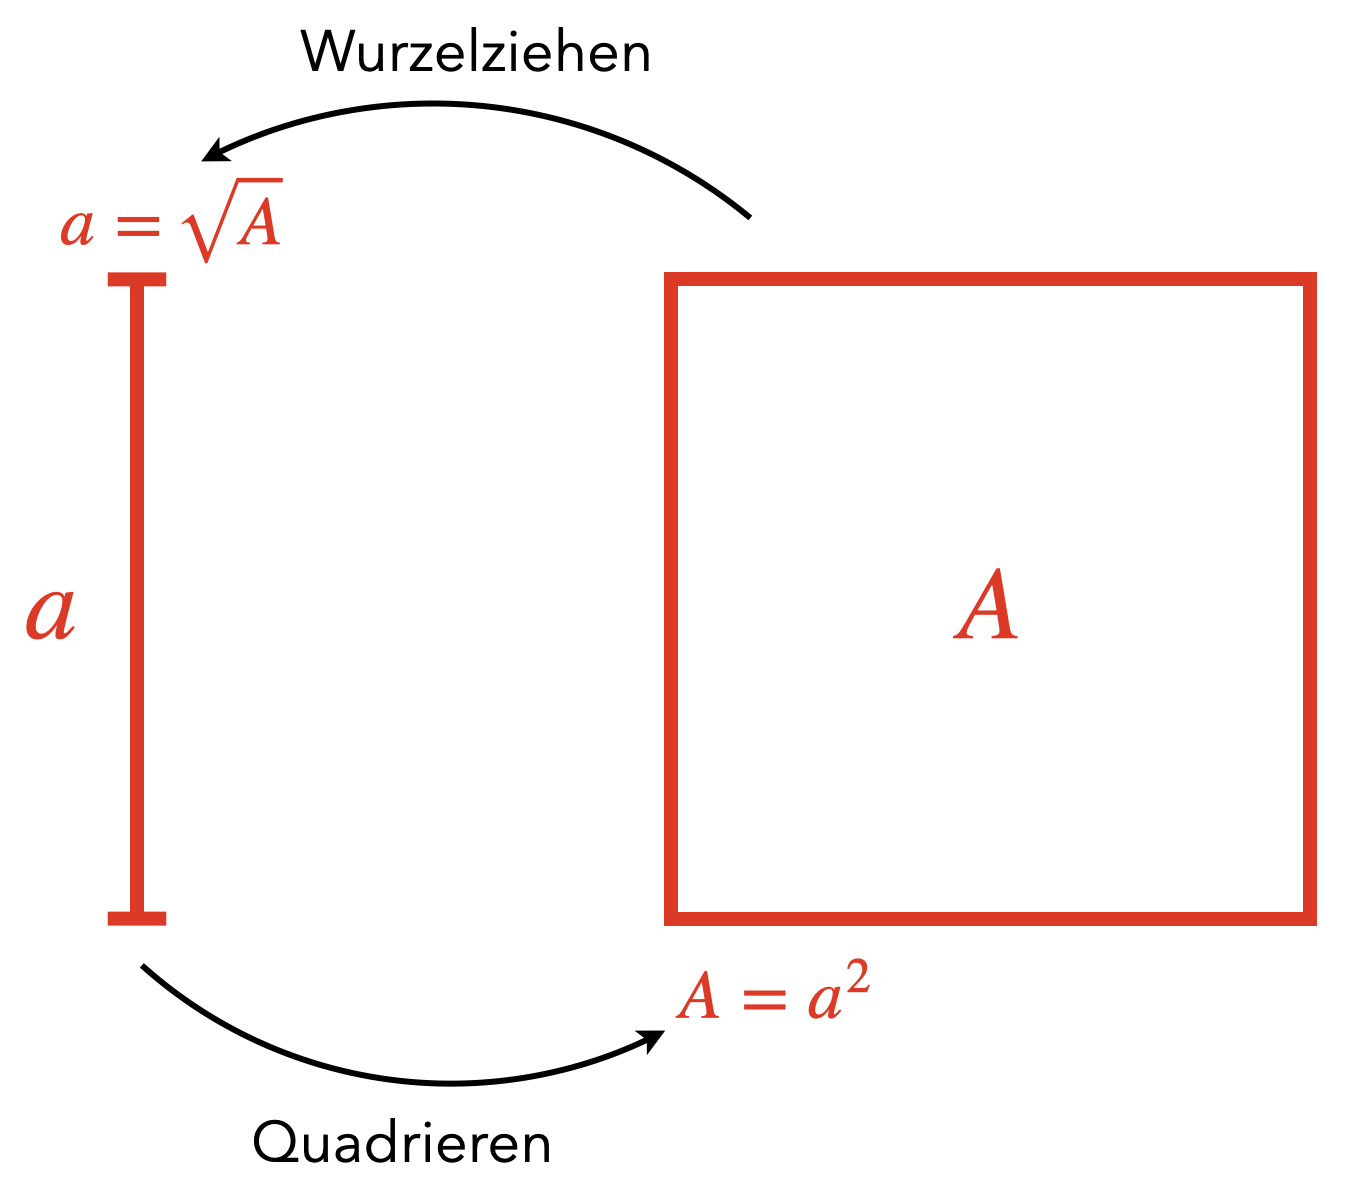
\includegraphics[width=0.5\linewidth]{pictures/8-Lernmodell} 

   }

   \caption{(ref:citeLernmodellWurzel)}\label{fig:LernmodellWurzel}
   \end{figure}

  \emph{Achtung! Es ist zwar \((-3)^2 = 9\), aber \(\sqrt{9} \neq -3\), da \(-3\) negativ ist. Außerdem ist \(\sqrt{-9}\) nicht definiert, da \(-9\) negativ ist.}

  In der Definition werden beschreibende Elemente mit der ikonischen und symbolischen Darstellungsebene in Bezug gebracht. Abbildung \ref{fig:LernmodellWurzel} kann gleichzeitig als \textbf{Lernmodell} aufgefasst werden: Sie veranschaulicht den Begriff und stellt gleichzeitig dar, wie zum Begriff gelangt werden kann. Damit liefert sie auch eine anschauliche Orientierung, wie das näherungsweise Bestimmen von Wurzeln über das Einbeschreiben von Quadraten erfolgen kann (siehe Abbildung \ref{fig:IntervallWurzel}).

  \begin{figure}

   {\centering 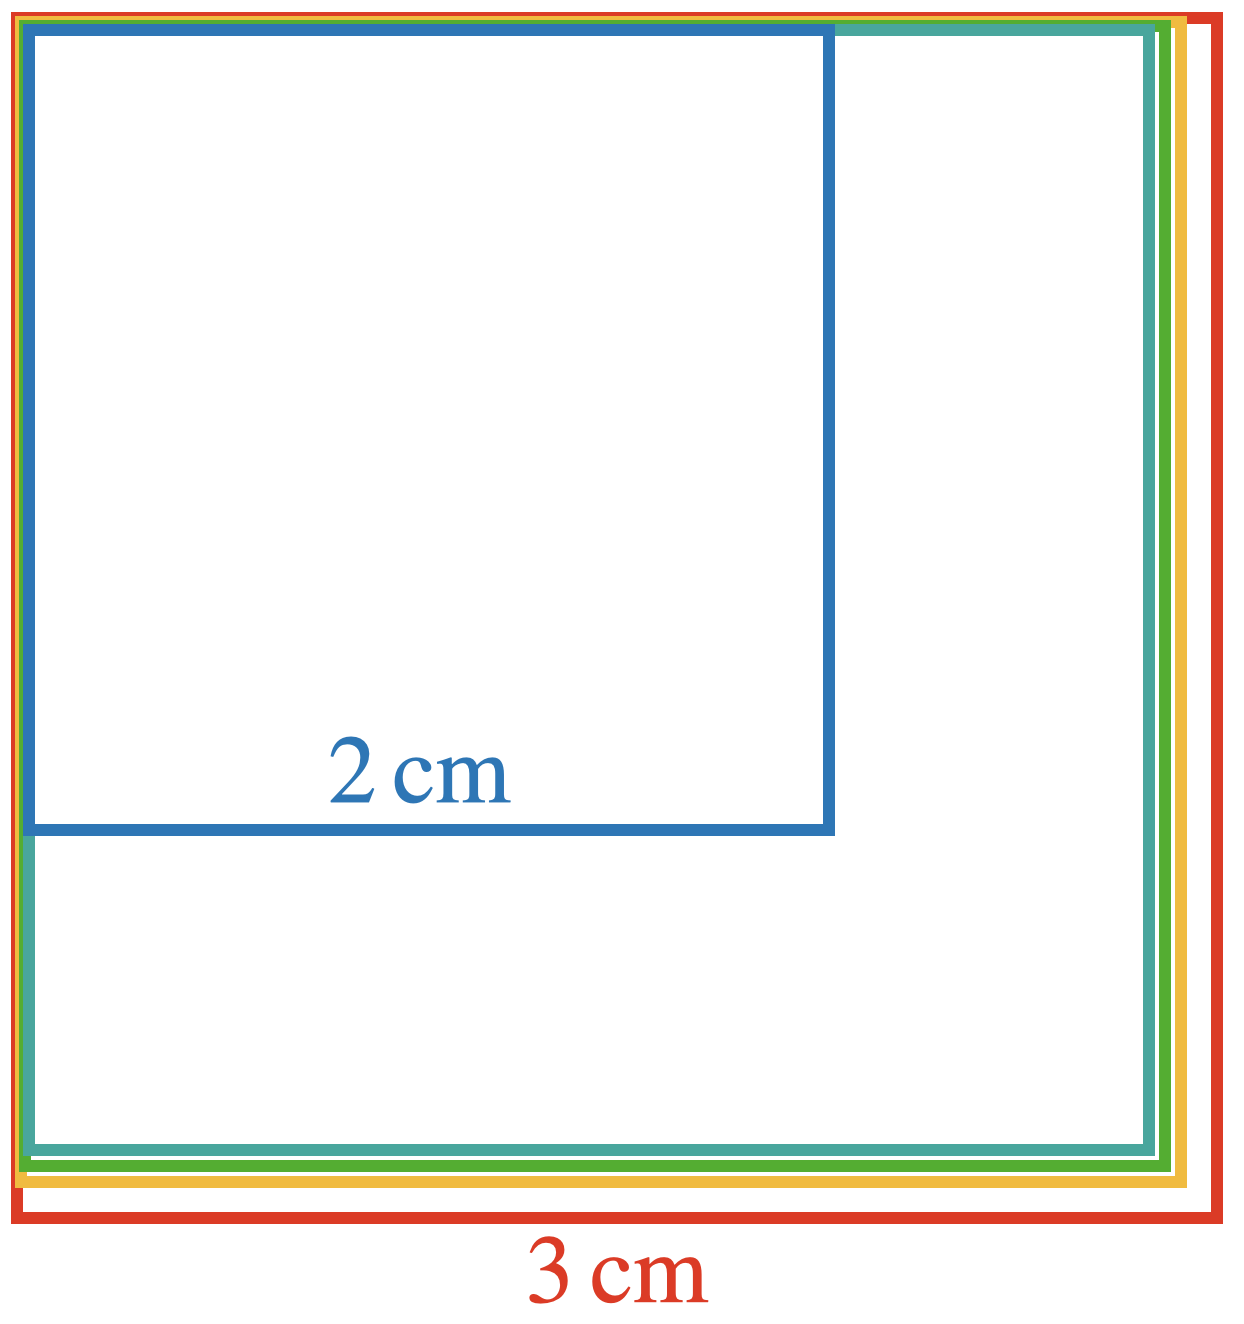
\includegraphics[width=0.25\linewidth]{pictures/8-Intervall} 

   }

   \caption{Nutzung des Lernmodells für die Intervallschachtelung}\label{fig:IntervallWurzel}
   \end{figure}

  Auch die Auswahl des \textbf{Beispiels} \(\sqrt{9}=3\) war nicht zufällig. Als Einstiegsbeispiel sollte ein leicht nachvollziehbares gewählt werden, daher sollte es sich um (möglichst kleine) natürliche Zahlen handeln und nicht mit Einheiten agiert werden. \(\sqrt{0}\) und \(\sqrt{1}\) fallen weg, da dies Spezialfälle sind, in denen die Werte für Wurzel und Quadrat identisch sind. \(\sqrt{4}\) ist ebenfalls ungünstig, weil dann bei der Erklärung der Umkehrung \(2^2 = 4\) die Ziffer \(2\) doppelt (und in verschiedenen Funktionen) auftaucht, nämlich als Basis und als Exponent. Um derartige \emph{Anfangsverwirrungen} zu vermeiden, ist dann \(\sqrt{9}\) das nächstliegende Einstiegsbeispiel. Entsprechend dem Kontrastprinzip müssen auch nahe \textbf{Gegenbeispiele} wie \(\sqrt{-9}\) sowie \(\sqrt{9}\neq -3\) gebracht werden. Das Variationsprinzip für die Auswahl von Beispielen kann über die verschiedenen Quadrate am Ausgangskonkretum erfüllt werden, in dem dort etwa nicht nur natürliche Zahlen auftreten.
\item
  Im letzten Schritt folgt das \textbf{Abarbeiten von Konkretisierungsreihen}, anhand derer das Ausgangsabstraktum tiefer durchdrungen wird.

  \begin{itemize}
  \item
    Beim Wurzelbegriff geht dies insbesondere mit der Zahlbereichserweiterung in die reellen Zahlen einher. Dabei werden Wurzeln als Zahlen (und nicht Seitenlängen) aufgefasst und bspw. auch auf dem Zahlenstrahl geordnet.
  \item
    Eine weitere charakteristische Anwendung der Lernhandlungen am Lernmodell ist bei der Betrachtung des Wurzelgesetzes \(\sqrt{x\cdot y} = \sqrt{x}\cdot \sqrt{y}\) möglich. Wird die Wurzel als \emph{Aufforderung} verstanden, zu einem Flächeninhalt die Seitenlänge des zugehörigen Quadrates zu finden, kann man den Term \(\sqrt{9\cdot 5}\) auffassen als die Suche nach der Seitenlänge des Quadrates mit dem \(9\)-Fachen des Flächeninhalts von \(5\,\mathrm{cm}^2\). Geometrisch interpretiert und angelehnt ans Lernmodell kann dies als ein Quadrat von Quadraten dargestellt werden (siehe Abbildung \ref{fig:QuadratQuadrat}). Dann ist die gesuchte Seitenlänge gerade das \(\sqrt{9}\)-Fache der Seitenlänge des Quadrates mit \(5\,\mathrm{cm}^2\) Flächeninhalt, also \(\sqrt{9\cdot 5} = \sqrt{9}\cdot \sqrt{5}\). Dies ist natürlich nur eine Plausibilitätsbetrachtung. Eine Begründung ist dann aber ebenfalls mithilfe der Definition über die Umkehrung und Nutzung der Potenzgesetze möglich: \(x^2\cdot y^2 = (x\cdot y)^2\).
  \end{itemize}

  \begin{figure}

    {\centering 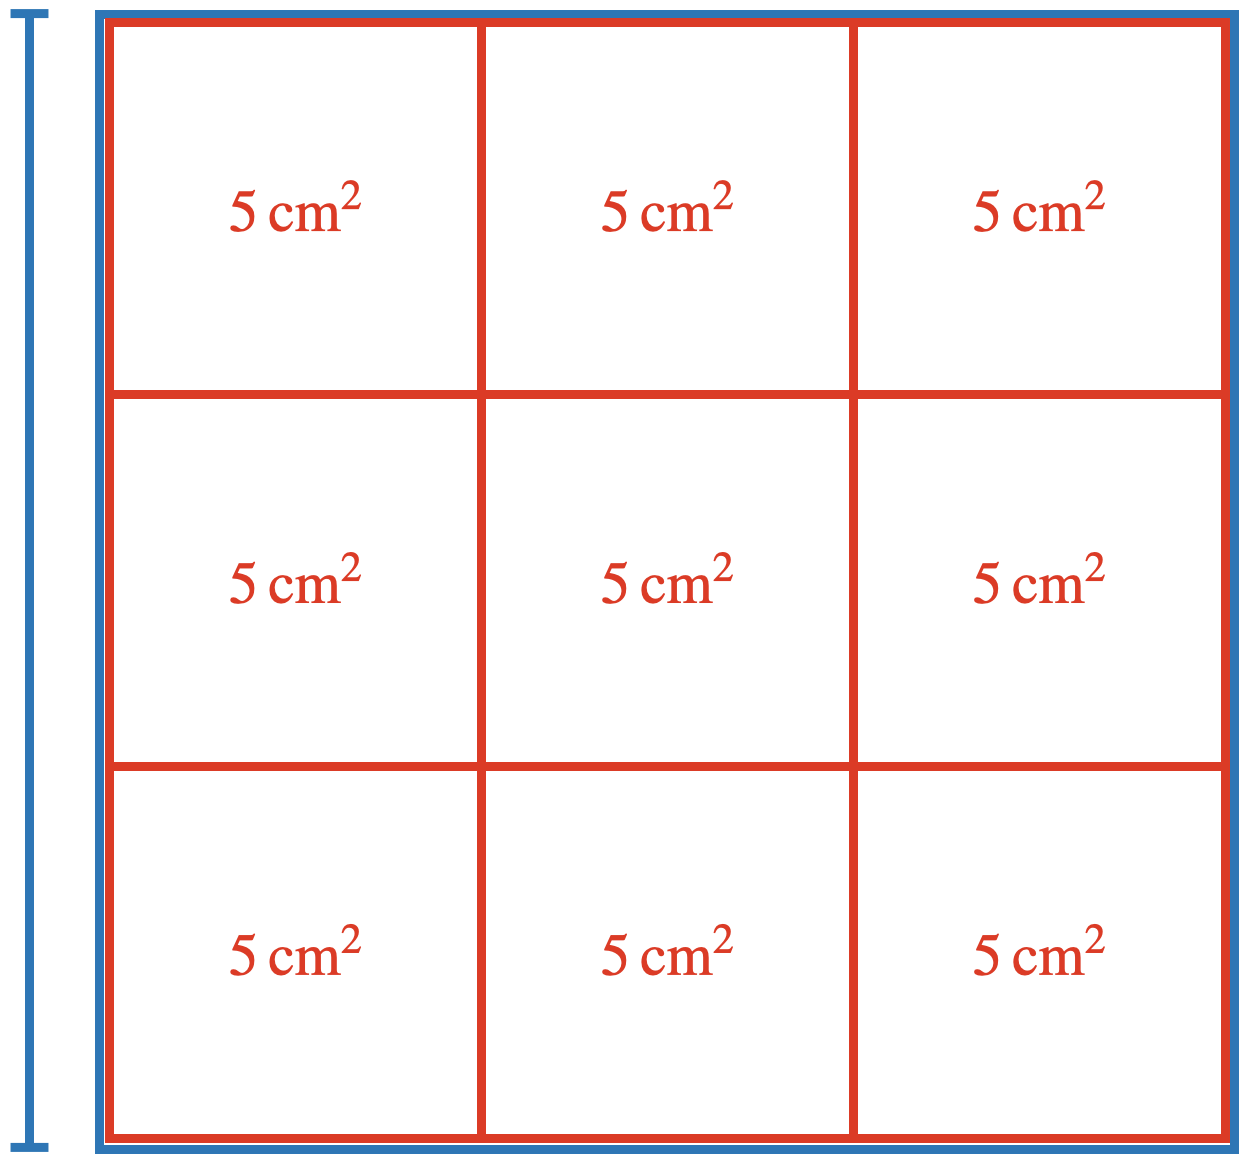
\includegraphics[width=0.5\linewidth]{pictures/8-QuadratQuadrat} 

    }

    \caption{Nutzung des Lernmodells für Quadrate von Quadraten}\label{fig:QuadratQuadrat}
    \end{figure}
\end{enumerate}

Wie nun aber konkrete Aufgaben und Lernumgebungen gestaltet werden können, die bspw. die Lernprozesse vom Ausgangskonkretum zum Ausgangsabstraktum bzw. zum Abarbeiten der Konkretisierungsreihen unterstützen, soll im weiteren Verlauf der Veranstaltung geklärt werden.

\hypertarget{zweites-intermezzo-nachbereitung}{%
\section{Zum Nachbereiten}\label{zweites-intermezzo-nachbereitung}}

Relektieren Sie, inwieweit das Vorgehen beim \protect\hyperlink{erstes-intermezzo-flaecheninhalt}{Ersten Intermezzo zum Flächeninhalt} über das Aufsteigen vom Abstrakten zum Konkreten realisiert werden kann und was dabei insbesondere das \emph{Ausgangskonkretum}, die \emph{Lernhandlungen}, das \emph{Lernmodell} und die \emph{Ausgangsabstraktion} sein können.

\hypertarget{part-unterrichtsgestaltung}{%
\part*{Unterrichtsgestaltung}\label{part-unterrichtsgestaltung}}
\addcontentsline{toc}{part}{Unterrichtsgestaltung}

\hypertarget{lernumgebungen}{%
\chapter*{Lernumgebungen}\label{lernumgebungen}}
\addcontentsline{toc}{chapter}{Lernumgebungen}

Mit den Kapiteln \ref{fundamentale-ideen} bis \ref{zweites-intermezzo-wurzel} haben Sie Ansätze kennengelernt, die Fragen der \textcolor{formalColor}{formalen}, \textcolor{semanticColor}{semantischen} und \textcolor{concreteColor}{konkreten} Ebene des \protect\hyperlink{tab:fragen-ebenen}{Vier-Ebenen-Ansatzes} nach \protect\hyperlink{ref-Hussmann:2016}{Hußmann \& Prediger} (\protect\hyperlink{ref-Hussmann:2016}{2016}) zu beantworten. Mit der deskriptiven Perspektive auf Grundvorstellungen kennen Sie auch schon erste Grundlagen, Fragen der \textcolor{empiricColor}{empirischen} Ebene zu untersuchen. Ziel bei all den Fragen war immer, \textbf{Lernpfade} für Lerngegenstände zu generieren, also den Stoff derart auszuwählen (\emph{spezifizieren}) und anzuordnen (\emph{strukturieren}), dass er sinnstiftend gelehrt und gelernt werden kann. Nach einer solchen \textbf{stoffdidaktischen Analyse} ist nun der nächste Schritt die Planung der Unterrichtsgestaltung an sich.

In der fachdidaktischen und bildungswissenschaftlichen Literatur hat sich hierfür der Begriff der \textbf{Lernumgebung} durchgesetzt -- dabei aber auch mit verschiedenen Sichtweisen wie eine »pädagogische« (z.~B. angenehme Lernatmosphäre, respektvolles Miteinander), als ein »methodisch-organisatorisches Arrangement« (z.~B. Gestaltung des Klassenraums) oder eben auch als »inhaltliches Verständnis«, das hier weiter verfolgt werden soll (vgl. \protect\hyperlink{ref-Krauthausen:2018}{Krauthausen, 2018, S. 255}).

Nach \protect\hyperlink{ref-Leuders2015}{Leuders} (\protect\hyperlink{ref-Leuders2015}{2015, S. 448}) beinhalten Lernumgebungen für den Mathematikunterricht \textbf{»i) ein nach bestimmten Prinzipien geordnetes System von Aufgaben, ii) methodische Organisationsformen und iii) Stützsysteme, wie z.~B. Medien, Lehrerinterventionen und Kommunikationsformen.«}

Die Grundlagen für die entsprechenden Bestandteile lernten und lernen Sie v.~a. in den weiteren Veranstaltungen der Fachdidaktiken und Bildungswissenschaften sowie in Ihrer schulpraktischen Ausbildung (und auch noch während Ihrer Tätigkeit als voll ausgebildete Lehrkraft). Aufgrund der inhaltlichen Nähe zur Stoffdidaktik-Veranstaltung sollen hier noch zwei Schwerpunkte herausgegriffen werden:

\begin{itemize}
\item
  Von den \emph{Medien} (zu denen ja beispielsweise auch die Tafel, Computer oder Zettel und Stift gehören -- der entsprechende Medienbegriff sollte Ihnen aus den Bildungswissenschaften bekannt sein) werden im Speziellen \textbf{Arbeitsmittel}\footnote{In der englischsprachigen Literatur werden \emph{Arbeitsmittel} oft als \emph{manipulatives} bezeichnet. Dies soll nicht ausdrücken, dass diese Arbeitsmittel in irgendeiner Weise manipulierend auf die Schülerin oder den Schüler wirken, sondern dass die Schülerinnen und Schüler selbst das Arbeitsmittel verändern bzw. mit dessen Hilfe auf den Lerngegenstand einwirken (siehe auch \protect\hyperlink{ref-enwiki:1023437370}{Wikipedia contributors, 2021}).} herausgegriffen. Diese »repräsentieren mathematische Objekte und erlauben zudem Handlungen oder Operationen mit diesen Objekten« (\protect\hyperlink{ref-Schmidt-Thieme2015}{Schmidt-Thieme \& Weigand, 2015, S. 461~f.}) Im Sinne der Tätigkeitstheorie dienen sie damit als Mittler zwischen Lerngegenstand und Schülerin bzw. Schüler. Im Schulalltag wird es in der Regel Ihre Aufgabe sein, derartige Arbeitsmittel zu \textbf{analysieren}, um sie zielgerichtet auszuwählen und im Unterricht einzusetzen. Das Herstellen entsprechender Arbeitsmittel bleibt meist die Aufgabe der fachdidaktischen Forschung und Entwicklung. Vorschläge, um Arbeitsmittel zu analysieren, finden Sie in Kapitel \ref{arbeitsmittel-analysieren}.
\item
  Eng verbunden mit dem Einsatz von Arbeitsmitteln sind \textbf{Aufgaben}, die Sie den Schülerinnen und Schülern stellen. Aufgaben können dabei »als Aufforderung an Lernende zum mathematischen Handeln aufgefasst« werden (\protect\hyperlink{ref-Leuders2015}{Leuders, 2015, S. 435}). Neben der Auswahl von Aufgaben werden Sie als Lehrkraft aber insbesondere Aufgaben \textbf{gestalten}, also selbst welche entwickeln und vorhandene Aufgaben variieren und an Ihre Lerngruppe anpassen. Maßnahmen, um Aufgaben zu gestalten, sind in Kapitel \ref{aufgaben-gestalten} dargestellt.
\end{itemize}

\hypertarget{arbeitsmittel-analysieren}{%
\chapter{Arbeitsmittel analysieren}\label{arbeitsmittel-analysieren}}

\begin{quote}
\textbf{Lernziele}

\begin{itemize}
\tightlist
\item
  Sie kennen ein Instrument zur Analyse von Arbeitsmitteln.
\item
  Sie können das Analyseinstrument tätigkeitstheoretisch einordnen.
\item
  Sie sind, ggf. mit Unterstützung, in der Lage, den Analyseprozess für Arbeitsmittel durchzuführen.
\end{itemize}

\textbf{Material}

\begin{itemize}
\tightlist
\item
  Folien zur Vorlesung zur Analyse von Arbeitsmitteln (\href{files/Stoffdidaktik-WiSe2122-Kap9.pdf}{pdf}, \href{files/Stoffdidaktik-WiSe2122-Kap9.key}{Keynote})
\end{itemize}
\end{quote}

\hypertarget{acat-modell}{%
\section{ACAT-Modell}\label{acat-modell}}

Um Arbeitsmittel (fundiert) analysieren zu können, sollte sich diese Analyse auf eine zugrundliegende Theorie (über das Lernen und Lehren) stützen und strukturiert ablaufen. Ein Vorschlag hierfür bietet das auf die Tätigkeitstheorie aufbauende Modell \textbf{Artifact-Centric Activity Theory (ACAT)}\footnote{übersetzt: Artefakt-zentrierte Tätigkeitstheorie} von \protect\hyperlink{ref-Ladel2013}{Ladel \& Kortenkamp} (\protect\hyperlink{ref-Ladel2013}{2013}), siehe Abbildung \ref{fig:ACAT}.



\begin{figure}

{\centering 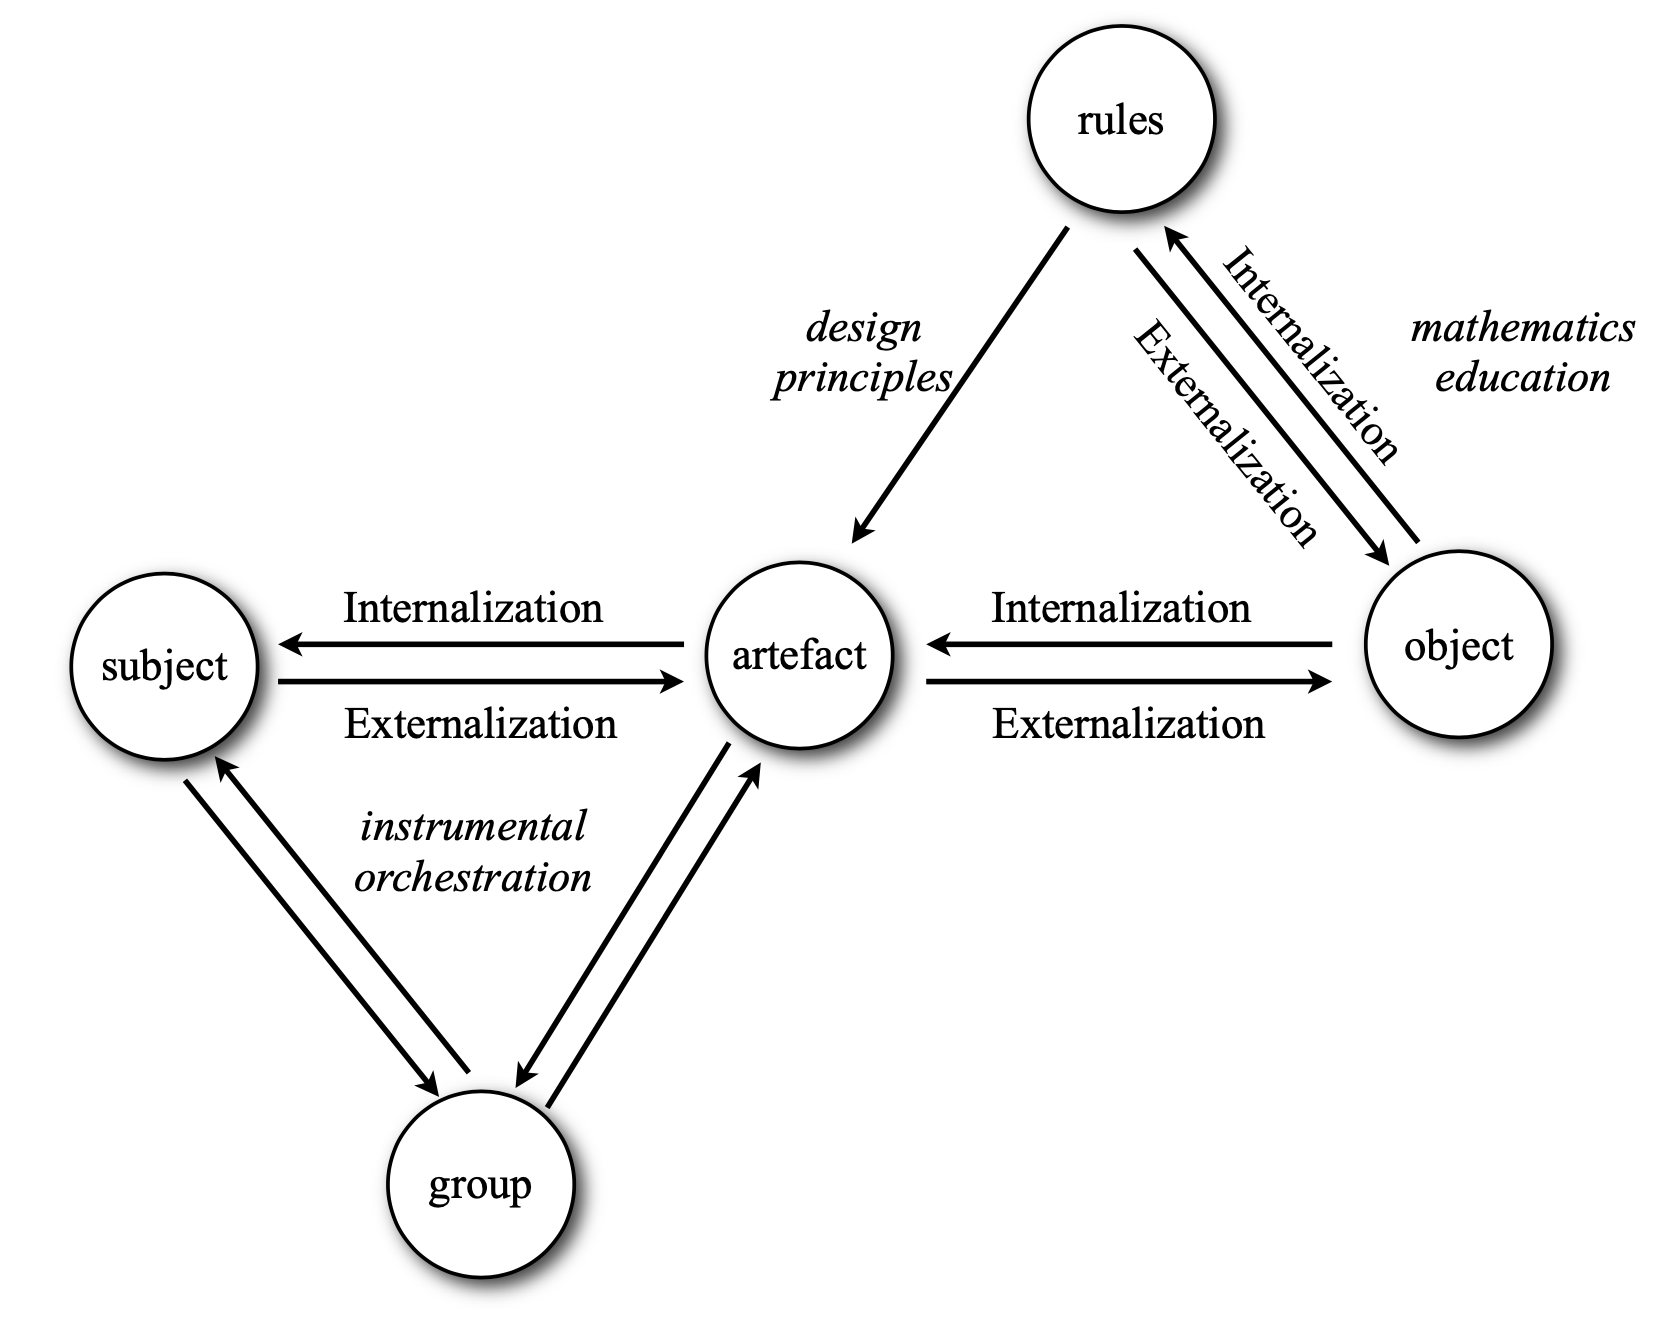
\includegraphics[width=0.75\linewidth]{pictures/9-ACAT} 

}

\caption{ACAT-Modell nach \protect\hyperlink{ref-Ladel2013}{Ladel \& Kortenkamp} (\protect\hyperlink{ref-Ladel2013}{2013, S. 4})}\label{fig:ACAT}
\end{figure}

Zunächst einmal ist auf der Hauptachse das Beziehungsgefüge aus Subjekt, Objekt und Artefakt dargestellt, das eine Grundannahme der Tätigkeitstheorie darstellt (siehe Abschnitt \ref{grundannahmen}). Es ist hier jedoch von einem \emph{Artefakt} die Rede. Damit soll ausgedrückt werden, dass es sich um ein künstlich geschaffenes Medium handelt, das zum Zwecke des Wissenserwerbs von einer mit dem Lerngegenstand vertrauten Person (z.~B. Lehrkraft oder Forscherin bzw. Forscher) entwickelt worden ist. Erst mit dem tatsächlichen und zielgerichteten Einsatz durch die Schülerinnen und Schüler wird es zum \emph{Werkzeug}, weil erst dann Internalisierungs- und Externalisierungsprozesse stattfinden.\footnote{Die Entwicklung vom Artefakt zum Werkzeug wird auch als \emph{Instrumentelle Genese} bezeichnet (vgl. \protect\hyperlink{ref-Etzold2021}{Etzold, 2021, S. 101~f.}).} Diese \emph{Internalisierung- und Externalisierungsprozesse} werden hier im Modell auf der Hauptachse dargestellt.

Das obere rechte Dreieck beschreibt die spezifische Gestaltung des Artefakts über sogenannte \emph{Regeln}. Die Regeln ergeben sich einerseits aus dem mathematischen Gegenstand selbst. Andererseits stammen sie aus weiteren Wissenschaftsbereichen wie der Psychologie, allgemeinen Didaktik, Multimedia-Design usw. und wirken wieder zurück auf das mathematische Objekt, indem die Regeln einen Einfluss darauf haben, welche Eigenschaften des Objektes repräsentiert werden. Wenn beispielsweise ein Spielwürfel aus Design-Gründen abgerundete Ecken und Kanten hat (damit sich die spielenden Kinder nicht verletzen), kann sich dies auf ein (falsches) mathematisches Verständnis des Würfel-Begriffs auswirken. Daher ist ein solcher Spielwürfel ungeeignet als Arbeitsmittel für den Erstkontakt mit dem entsprechenden Begriff. Aus den Regeln heraus wird das Artefakt gestaltet.

Im unteren linken Dreieck wird nun der Einsatz des Artefakts in der \emph{Klassensituation} dargestellt. Hierbei spielen z.~B. konkrete Aufgabenstellungen eine Rolle, die die Schülerinnen und Schüler zur zielgereichteten Arbeit mit dem Artefakt anregen. Auch ist die Rolle der Lehrkraft im Lehr-Lern-Prozess von Bedeutung, ebenso wie die methodische Ausgestaltung der Artefakt-Nutzung, ggf. auch im Zusammenspiel mit weiteren Artefakten. Dieses komplexe Beziehungsgefüge wird auch als \emph{instrumental orchestration} bezeichnet (siehe z.~B. \protect\hyperlink{ref-Drijvers2010}{Drijvers et al., 2010, S. 214~f.}).

\hypertarget{analyseschritte}{%
\section{Analyseschritte}\label{analyseschritte}}

\protect\hyperlink{ref-Larkin2019}{Larkin et al.} (\protect\hyperlink{ref-Larkin2019}{2019}) stellen dar, wie sich das ACAT-Modell als Analyseinstrument für Unterrichtsapps einsetzen lässt, eine Übersetzung des Beurteilungsleitfadens findet sich bei \protect\hyperlink{ref-Etzold2018}{Etzold et al.} (\protect\hyperlink{ref-Etzold2018}{2018}) und eine für Lehrkräfte angepasste Variante bieten \protect\hyperlink{ref-Kortenkamp2019}{Kortenkamp et al.} (\protect\hyperlink{ref-Kortenkamp2019}{2019}). Daran angelehnt bieten sich folgende Prozessschritte für die Analyse eines Arbeitsmittels an:

\begin{enumerate}
\def\labelenumi{\arabic{enumi}.}
\item
  \textbf{Identifizieren des mathematischen Objekts}

  Zunächst muss klar sein, für welches mathematische Objekt -- also für welchen Begriff, welchen Inhalt, welches Thema -- das Arbeitsmittel eingesetzt werden soll. Sind mehrere mathematische Objekte möglich, muss die Analyse auch für jedes getrennt erfolgen, da das Arbeitsmittel ggf. unterschiedlich gut geeignet sein kann. Theoretischer Hintergrund ist, dass \textbf{ohne Objekt keine zielgerichtete Handlung eines Subjekts möglich} ist. Daher können Handlungen von Schülerinnen und Schülern mit einem Arbeitsmittel nur dann bewertet werden, wenn Klarheit bezüglich des (mathematischen) Objekts besteht.

  \textbf{\emph{Mögliche Quellen}} hierfür sind die Bezeichnung des Arbeitsmittels bzw. eine offizielle Beschreibung, Zusatzmaterialien zum Arbeitsmittel (wie Arbeitsblätter, Handreichungen, \ldots), externe Referenzen (z.~B. Empfehlungen durch Dritte) oder auch das selbstständige Ausprobieren des Arbeitsmittels.
\item
  \textbf{Herausstellen der Interaktionsmöglichkeiten mit dem mathematischen Objekt über das Arbeitsmittel}

  Anschließend kann man sich Gedanken darüber machen, welche Interaktionsmöglichkeiten das Arbeitsmittel den Schülerinnen und Schülern mit dem mathematischen Objekt anbietet. Theoretischer Hintergrund hierfür ist, dass externe Handlungen des Subjekts (zum Beispiel eine \emph{pinch-to-zoom}-Geste zum Vergrößern oder Verkleinern einer Landkarte auf einem Tablet-Bildschirm) interne Handlungen wiederspiegeln (hier: zentrische Streckungen), die das Verständnis repräsentieren -- man spricht von \textbf{Externalisierung}. Ebenso führen externe Handlungen aber auch zum Aufbau interner Repräsentationen (hier z.~B.: Veränderung der Fingerposition zu Beginn der Handlung ändert das Streckungszentrum) -- man spricht von \textbf{Internalisierung}. Um diese Nutzerinteraktion besser zu verstehen und in Bezug auf das mathematische Objekt zu sehen, ist es hilfreich, den Prozess zwischen Subjekt und Objekt am Artefakt (dem Arbeitsmittel) aufzutrennen und in Teilfragen zu beantworten:

  \textbf{S → A:} Welche Handlungen sind mit dem Arbeitsmittel möglich?\\
  \textbf{A → O:} Wie repräsentiert das Arbeitsmittel das mathematische Objekt?\\
  \textbf{O → A:} Wie beeinflusst das Objekt das Verhalten des Arbeitsmittels?\\
  \textbf{A → S:} Welche Erfahrungen können Schülerinnen und Schüler dadurch machen?

  Eine \textbf{\emph{mögliche Quelle}} ist die eigene, systematische Nutzung des Arbeitsmittels.
\item
  \textbf{Analyse der Entwicklung der Interaktion}

  Nun werden die möglichen Interaktionen qualitativ strukturiert, um die mögliche Entwicklung des Lernens der Schülerinnen und Schüler besser zu beschreiben. Die Strukturierung bezieht sich auf die in der Tätigkeitstheorie übliche Unterscheidung in Tätigkeiten, Handlungen und Operationen:

  \begin{itemize}
  \tightlist
  \item
    \textbf{Tätigkeiten} sind übergeordnete, an \emph{Motiven} orientierte Interaktionen (z.~B. das Lesen einer Landkarte).
  \item
    \textbf{Handlungen} sind \emph{zielgerichtete}, individuelle Interaktionen, die die Tätigkeit realisieren (z.~B. das Vergrößern eines Kartenausschnittes, um diesen detaillierter betrachten zu können).
  \item
    \textbf{Operationen} sind zur Handlungsausführung notwendige Interaktionen, die jedoch kein weiteres Nachdenken erfordern und ggf. \emph{instrumentellen Zwängen} unterworfen sind (z.~B. das Ausführen der \emph{pinch-to-zoom}-Geste oder das Verschieben der Karte mit dem Finger).
  \end{itemize}

  In einem erfolgreichen Lernprozess verschieben sich (durch Verinnerlichungsprozesse) insbesondere Handlungen zu Operationen, um darauf neue, komplexere Handlungen aufbauen zu können. Es ist also darzustellen, wie eine dartige Entwicklung mithilfe des Arbeitsmittels unterstützt werden kann.

  \textbf{\emph{Mögliche Quellen}} sind hypothetische Diskussionen potenzieller Entwicklungen, aber auch empirische Untersuchungen.
\item
  \textbf{Überprüfung der Eignung des Arbeitsmittels für die Vermittlung des mathematischen Objekts}

  In diesem Schritt wird die Realisierung des Arbeitsmittels für das spezielle mathematische Objekt mit den Erkenntnissen aus Fachdidaktik, Fachwissenschaft und Psychologie verglichen. Dabei wird geprüft, ob die in den Schritten 2 und 3 analysierten Interaktionen tatsächlich die aus Sicht der Mathematik(-didaktik) erwünschten oder benötigten Vorstellungen, Erfahrungen und Kompetenzen unterstützen. Im ACAT-Modell entspricht dies der regelgeleiteten Gestaltung des Artefakts, wobei diese Regeln wiederum aus mathematikdidaktischen Überlegungen, allgemeinem Multimediadesign, usw. stammen.

  \textbf{\emph{Mögliche Quellen}} für diesen Schritt sind neben der Synthese der vorherigen Diskussionen v.~a. auch wissenschaftliche Referenzen und Veröffentlichungen.
\item
  \textbf{Möglichkeiten zur Verwendung des Arbeitsmittels in der Klassensituation }

  In einem letzten Schritt werden Möglichkeiten dargestellt, wie der Einsatz des Arbeitsmittels im Unterricht konkret aussehen kann. Folgende Fragen bieten eine Orientierung:

  \begin{itemize}
  \tightlist
  \item
    Ist das Arbeitsmittel für individuelle Arbeit, Partnerarbeit oder Kleingruppenarbeit geeignet?
  \item
    Was sind mögliche Impulse und Aufgabenstellungen, die Sie als Lehrerin oder Lehrer geben können?
  \item
    Welche Differenzierungsmaßnahmen und verschiedenen Schwierigkeitsgrade sind möglich?
  \item
    Handelt es sich um Übungsmaterial oder dient es zur Einführung neuer Lerninhalte und dem Aufbau von Grundvorstellungen?
  \item
    Welche Voraussetzungen/Kompetenzen werden an die Schülerinnen und Schüler für die Nutzung des Arbeitsmittels gestellt?
  \item
    Wie können Diskussionen bzw. Interaktionen innerhalb der Klasse mithilfe des Arbeitsmittels direkt oder indirekt gefördert werden?
  \end{itemize}

  Tätigkeitstheoretischer Hintergrund ist hierbei, dass Lernen niemals als eine rein individuelle Tätigkeit eines Schülers oder einer Schülerin angenommen wird, sondern immer im gesellschaftlichen und sozialen Kontext geschieht. Oder mit anderen Worten: »Im Unterricht agiert immer ein pädagogisches Gesamtsubjekt« (\protect\hyperlink{ref-Giest2004a}{Giest \& Lompscher, 2004, S. 112}).

  \textbf{\emph{Mögliche Quellen}} für derarbeite Überlegungen sind Materialien für Lehrerinnen und Lehrer, wissenschaftliche Ergebnisse, bspw. aus experimentellen Studien bzw. Versuchsdurchführungen im Unterricht.
\end{enumerate}

Diese fünf Schritte sprechen damit jeweils verschiedene Elemente des ACAT-Modells an. Abbildung \ref{fig:ACATAnalyse} fasst dies noch einmal zusammen.

\begin{figure}

{\centering 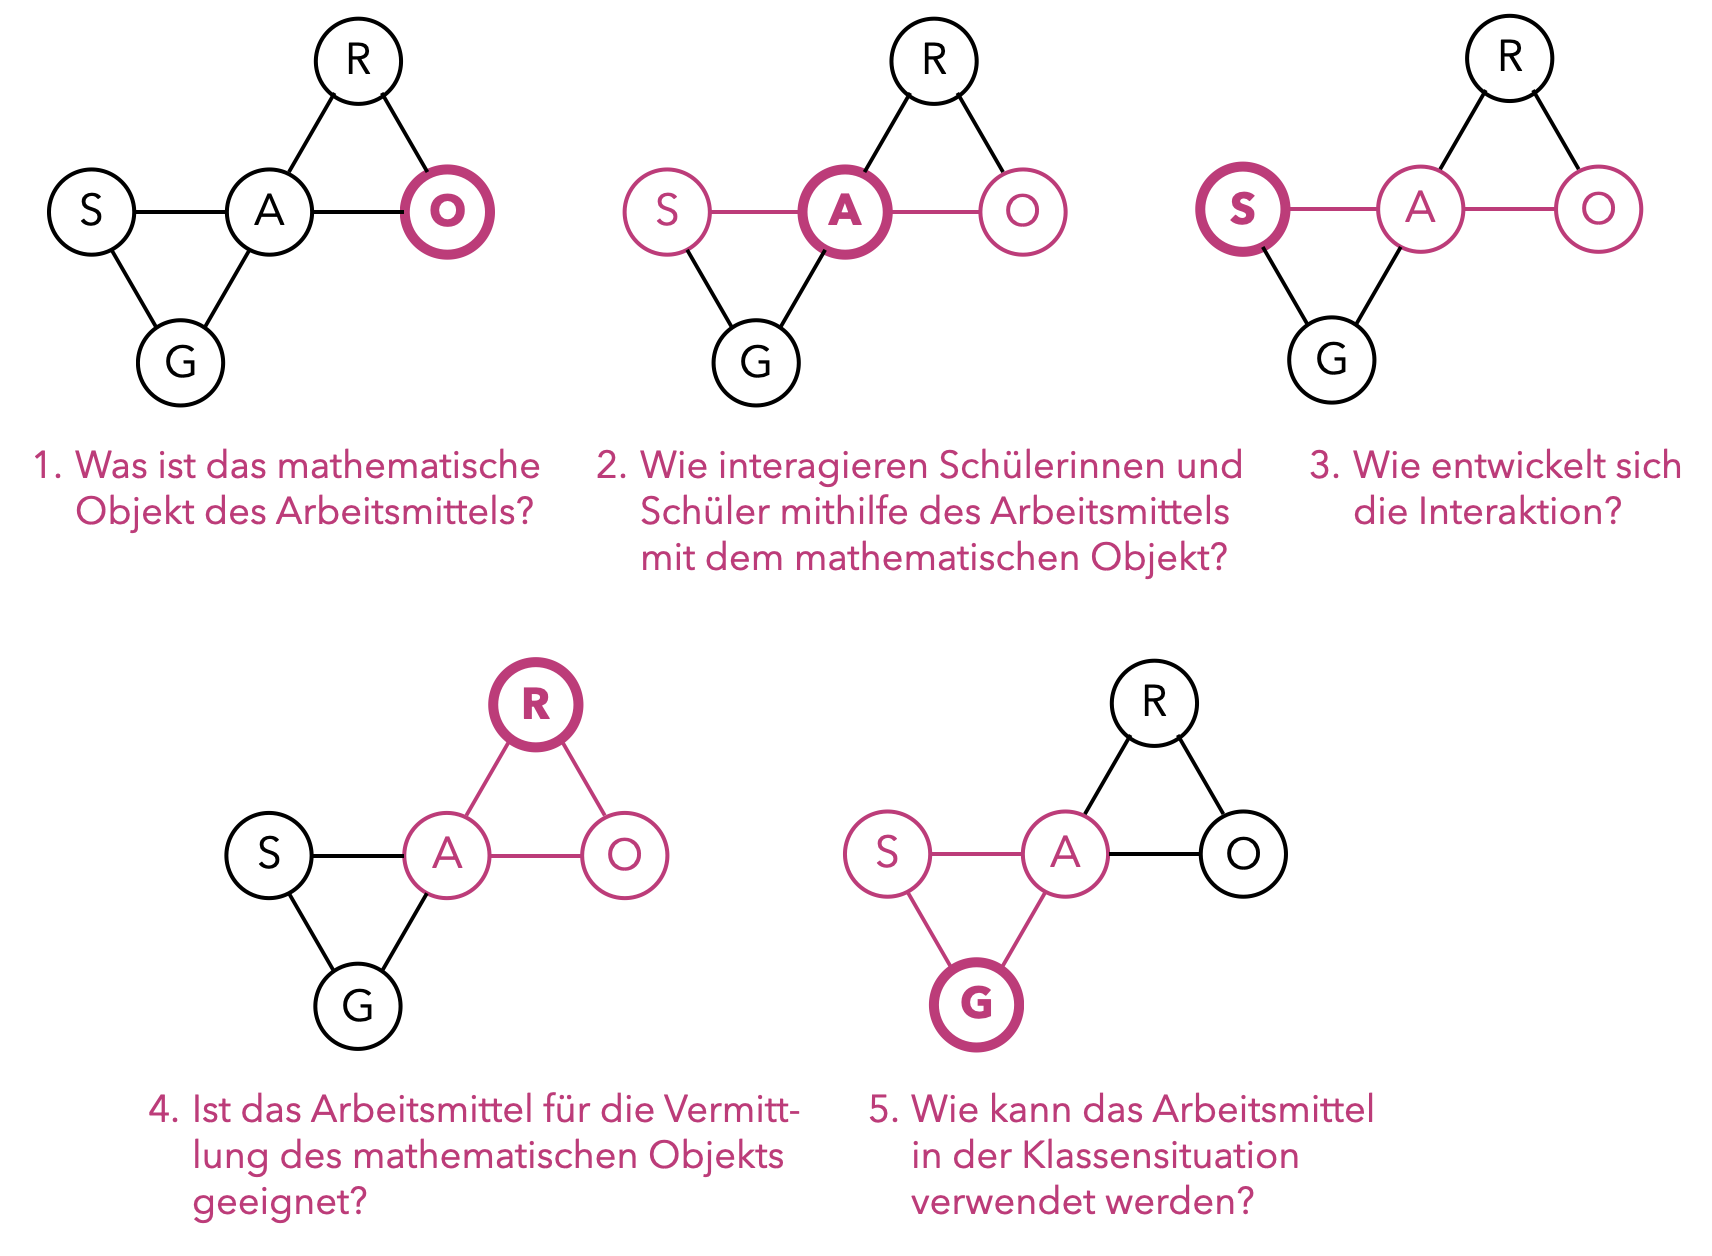
\includegraphics[width=0.9\linewidth]{pictures/9-ACATAnalyse} 

}

\caption{ACAT-Analysemodell für Arbeitsmittel}\label{fig:ACATAnalyse}
\end{figure}

Am Beispiel der App \emph{Klipp Klapp} (\protect\hyperlink{ref-Etzold2020a}{Etzold, 2020}) stellt \protect\hyperlink{ref-Stein2018}{Stein} (\protect\hyperlink{ref-Stein2018}{2018}) eine entsprechende Analyse dar, die englischsprachige Übersetzung ist bei \protect\hyperlink{ref-Larkin2019}{Larkin et al.} (\protect\hyperlink{ref-Larkin2019}{2019, S. 85~ff.}) zu finden.

Im Übrigen kann ein auf diese Weise als erfolgreich beurteiltes Arbeitsmittel den Charakter eines \emph{Lernmodells} annehmen, wie es im Abschnitts \ref{aufsteigen-vom-abstrakten-zum-konkreten} charakterisiert wird.

\hypertarget{arbeitsmittel-analysieren-nachbereitung}{%
\section{Zum Nachbereiten}\label{arbeitsmittel-analysieren-nachbereitung}}

\begin{enumerate}
\def\labelenumi{\arabic{enumi}.}
\item
  Lesen Sie als Hintergrundtheorie zur Analyse von Unterrichtsapps den Artikel von \protect\hyperlink{ref-Larkin2019}{Larkin et al.} (\protect\hyperlink{ref-Larkin2019}{2019}).
\item
  Führen Sie nach der hier vorgestellten Schrittfolge eine Analyse des Arbeitsmittels \emph{Zahlenstrahl} durch (siehe z.~B. auch \protect\hyperlink{ref-Schulz2018}{Schulz, 2018}).
\end{enumerate}

\hypertarget{aufgaben-gestalten}{%
\chapter{Aufgaben gestalten}\label{aufgaben-gestalten}}

\begin{quote}
\textbf{Lernziele}

\begin{itemize}
\tightlist
\item
  Sie kennen Möglichkeiten, Aufgaben je nach ihrer Funktion und den auszubildenden Fähigkeitsaspekten auszuwählen bzw. zu erstellen.
\item
  Sie können Aufgaben aus Schulbüchern für produktives Üben anpassen.
\item
  Sie kennen Differenzierungsmöglichkeiten mithilfe von Aufgaben und können differenzierende Aufgaben erstellen.
\end{itemize}

\textbf{Material}

\begin{itemize}
\tightlist
\item
  Folien zur Vorlesung zur Gestaltung von Aufgaben (\href{files/Stoffdidaktik-WiSe2122-Kap10.pdf}{pdf}, \href{files/Stoffdidaktik-WiSe2122-Kap10.key}{Keynote})
\end{itemize}
\end{quote}

In der Veranstaltung \emph{Einführung in die Mathematikdidaktik} lern(t)en Sie zentrale Aufgabentypen kennen, die Ihnen Aussage über die \emph{Offenheit} von Aufgaben liefern (siehe auch \protect\hyperlink{ref-Bruder}{Bruder, o.~J., S. 2}). Weiterhin wird an dieser Stelle davon ausgegangen, dass Sie \emph{Operatoren} kennen, die für eine präzise Formulierung von Aufgabenstellungen genutzt werden können (siehe auch \protect\hyperlink{ref-InstitutfurQualitatsentwicklungimBildungswesen2019}{Institut für Qualitätsentwicklung im Bildungswesen, 2019}; \protect\hyperlink{ref-MinisteriumfurBildungJugendundSportdesLandesBrandenburg}{Ministerium für Bildung, Jugend und Sport des Landes Brandenburg, 2015a, S. 11}).

\hypertarget{funktionen-von-aufgaben}{%
\section{Funktionen von Aufgaben}\label{funktionen-von-aufgaben}}

»Eine Aufforderung zum Lern-Handeln im Mathematikunterricht wird als \textbf{Aufgabe} bezeichnet« (\protect\hyperlink{ref-Bruder2012}{Bruder, 2012, S. 19}, Hervorhebung im Original). Mit diesem Aufgabenbegriff sind Sie nun als Lehrkraft gefordert, Ihre Schülerinnen und Schüler anzuregen, sich aktiv mit mathematischen Lerngegenständen auseinanderzusetzen. Dabei sollten Sie sich der verschiedenen möglichen \textbf{Funktionen von Aufgaben} bewusst sein, da dies jeweils die Art und Weise, wie Sie Aufgaben formulieren und sie im Unterricht einsetzen, beeinflussen (vgl. \protect\hyperlink{ref-Leuders2015}{Leuders, 2015, S. 439}; \protect\hyperlink{ref-SINUSBayern}{SINUS Bayern, o.~J.}). Die hier angebrachten Beispiele beziehen sich auf den Lerngegenstand \emph{Prozentrechnung}.











\begin{itemize}
\item
  Aufgaben können dem \textbf{Erkunden}, \textbf{Entdecken} und \textbf{Erfinden} dienen. Diese in der Regel am Anfang eines Themengebiets stehenden Aufgaben sollten möglich offen formuliert sein und in besonderer Weise Motivation schaffen, sich mit dem Lerngegenstand erstmals auseinanderzusetzen (siehe Abbildung \ref{fig:ProzentErkunden}). An dieser Stelle können auch typische W-Fragen gestellt werden -- es ist im Sinne der Offenheit nicht zwingend notwendig, sich an den Operatoren zu orientieren.

  \begin{figure}

    {\centering 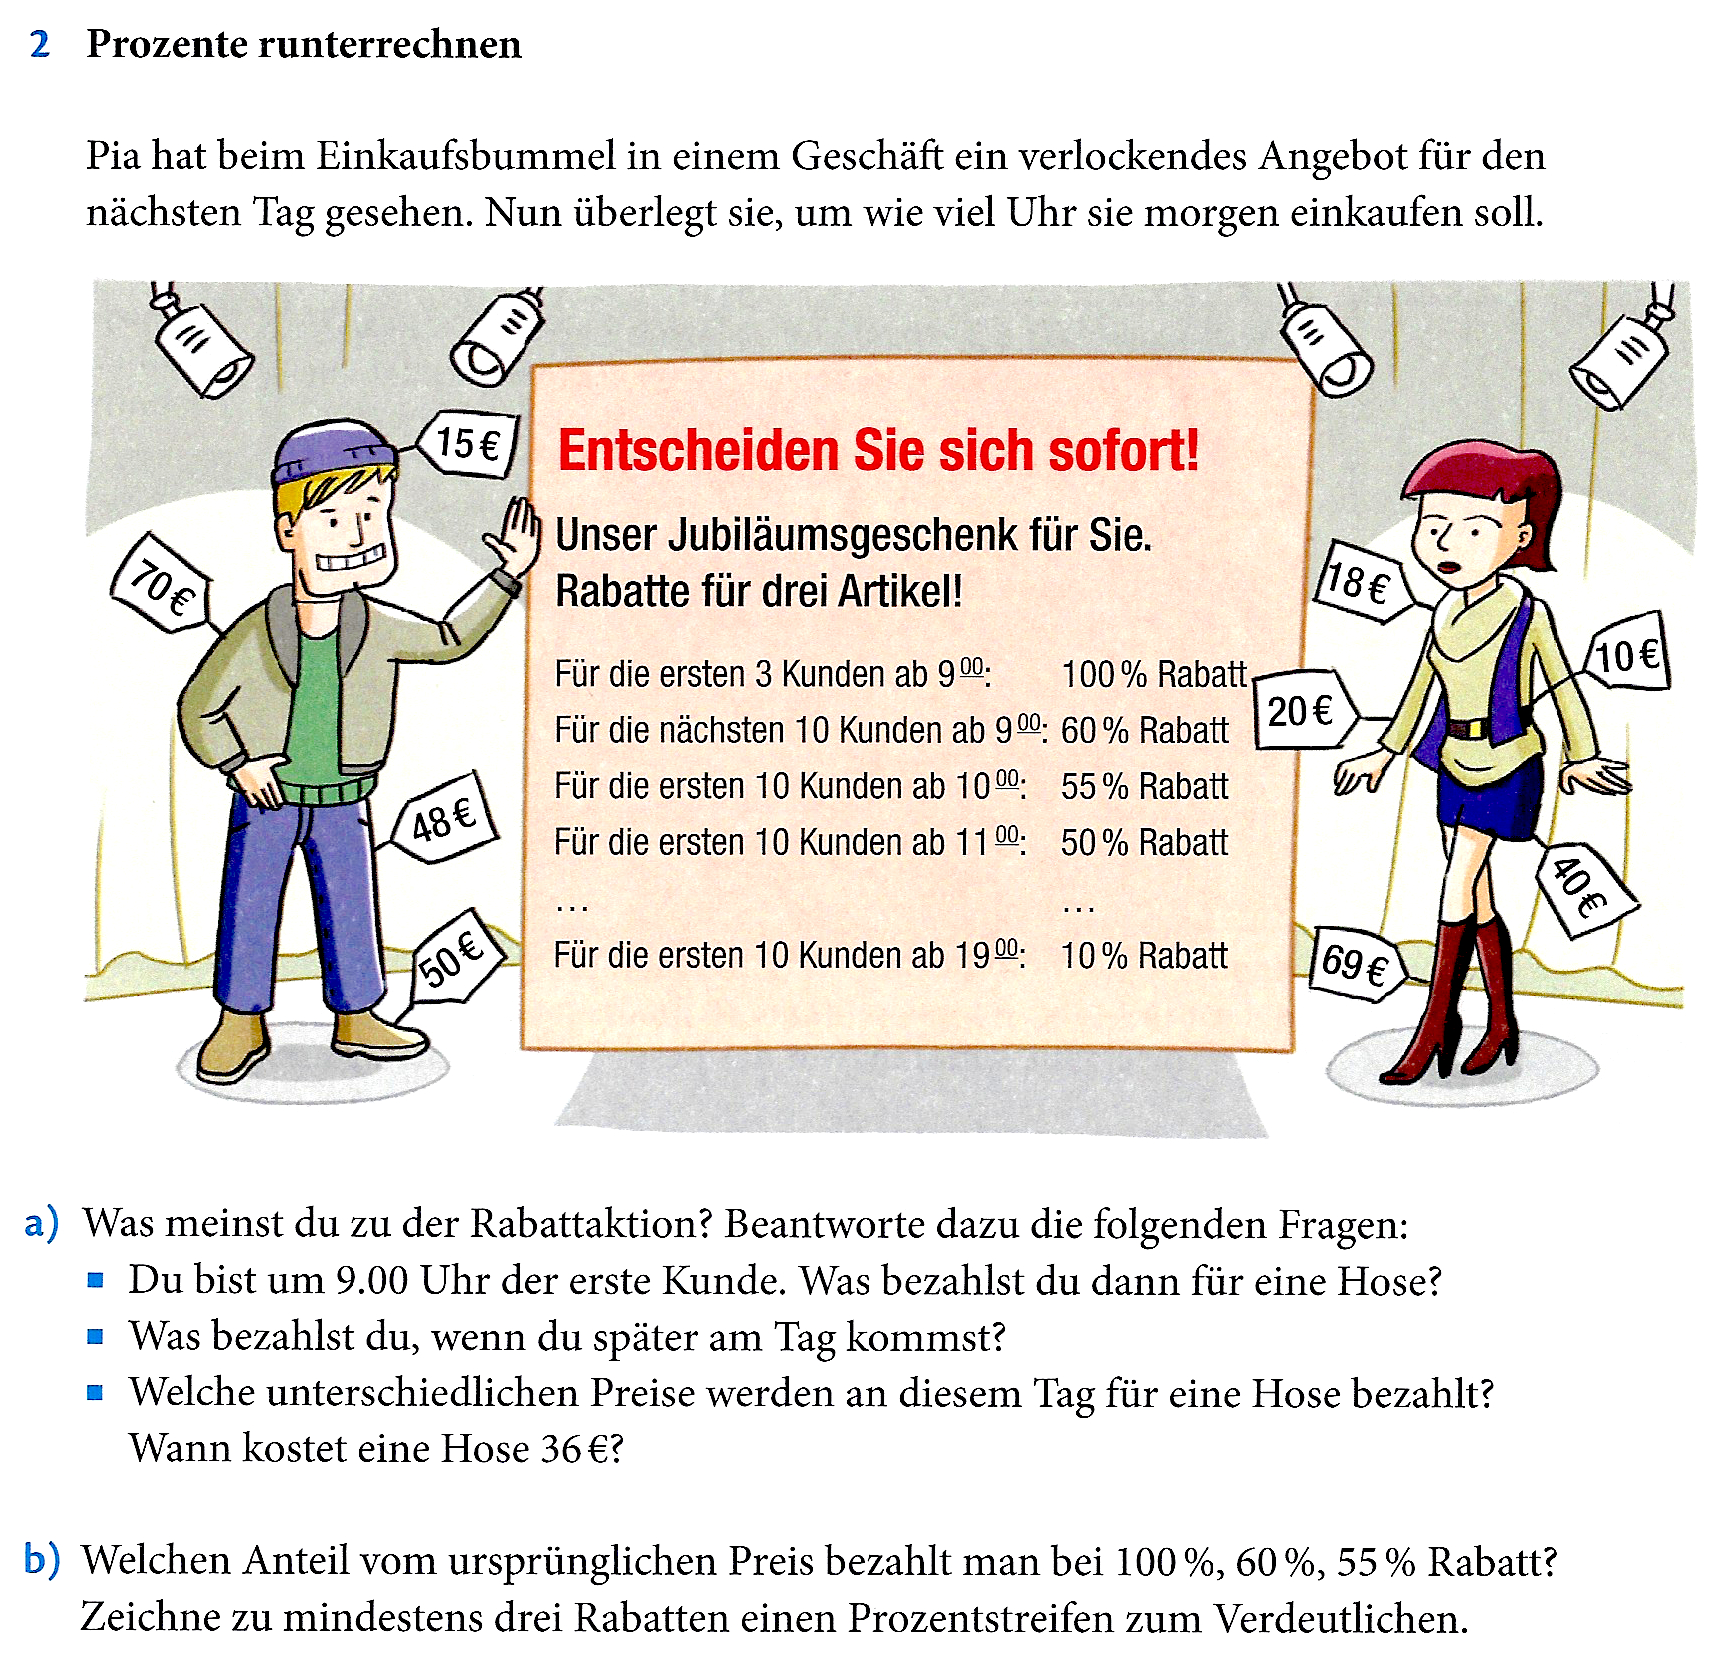
\includegraphics[width=0.75\linewidth]{pictures/10-ProzentErkunden} 

    }

    \caption{Erkundungsaufgabe zur Prozentrechnung (\protect\hyperlink{ref-Barzel2015a}{Leuders et al., 2015, S. 223})}\label{fig:ProzentErkunden}
    \end{figure}
\item
  Aufgaben zum \textbf{Sammeln}, \textbf{Sichern} und \textbf{Systematisieren} greifen vorherige Ideen auf, mit denen dann eine gewünschte mathematische Struktur herausgearbeitet werden soll (siehe Abbildung \ref{fig:ProzentSammeln}). In derartigen Aufgaben können Schülerinnen und Schüler auch angeleitet werden, sinnvolle Repräsentationen zu nutzen, um Grundvorstellungen auszubilden.

  \begin{figure}

    {\centering 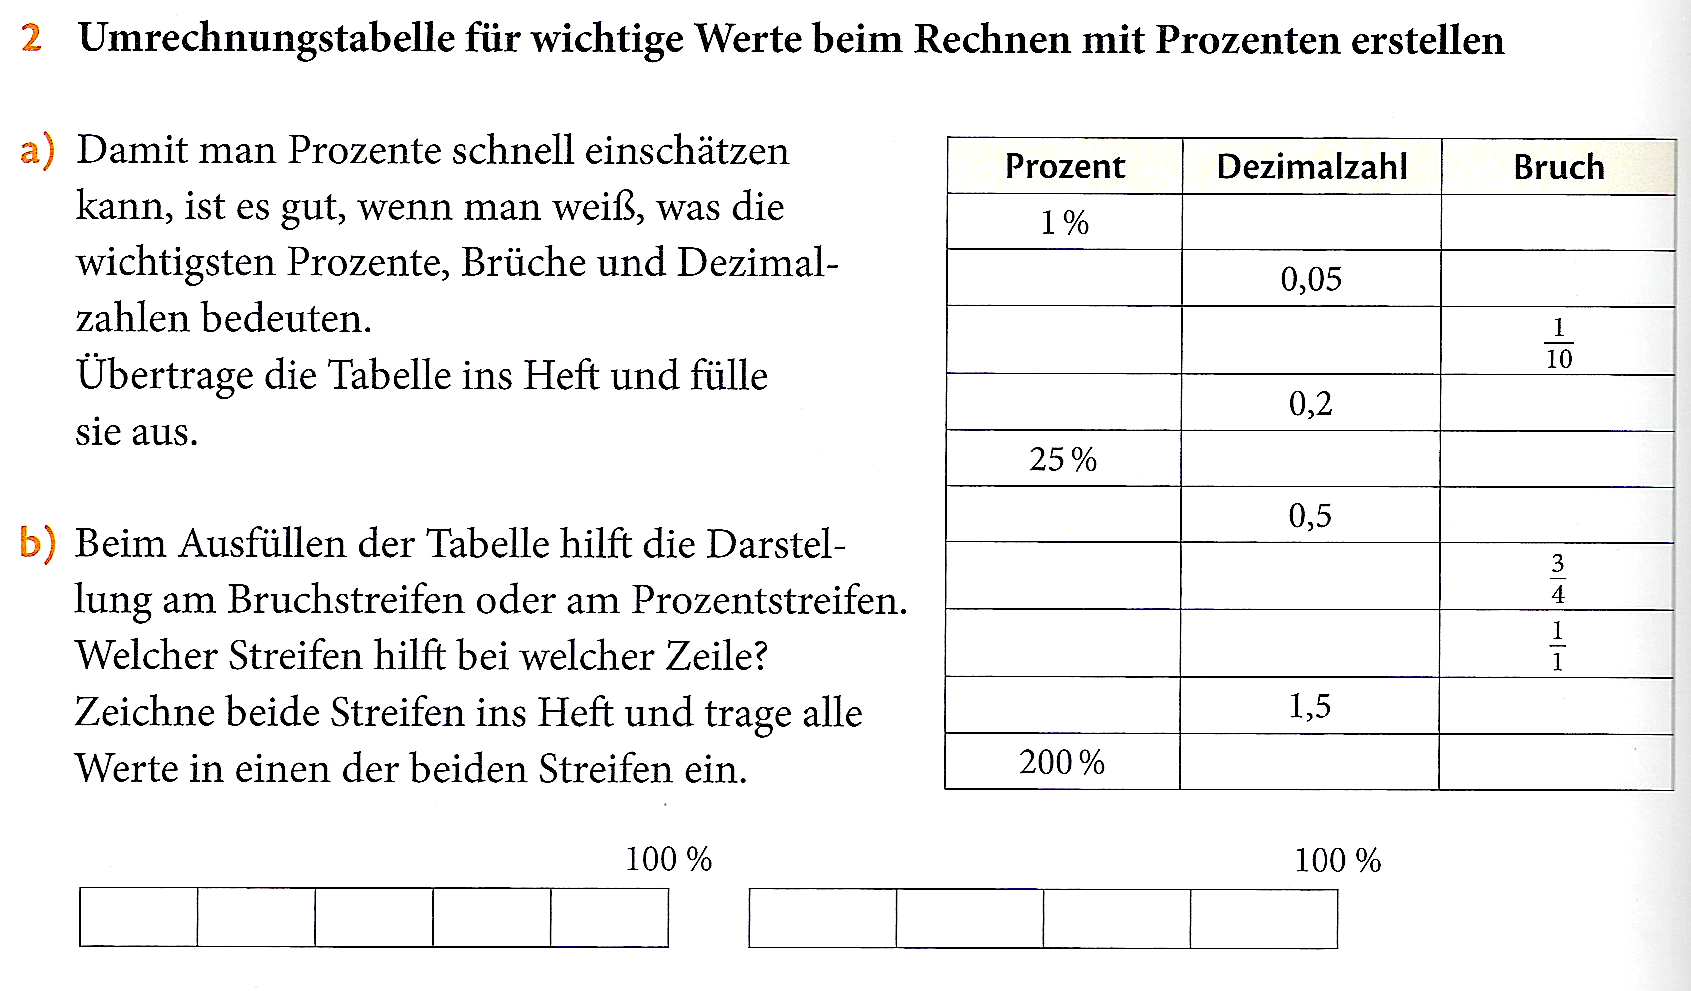
\includegraphics[width=0.75\linewidth]{pictures/10-ProzentSammeln} 

    }

    \caption{Systematisierungsaufgabe zur Prozentrechnung (\protect\hyperlink{ref-Barzel2015a}{Leuders et al., 2015, S. 226})}\label{fig:ProzentSammeln}
    \end{figure}
\item
  \textbf{Üben}, \textbf{Festigen} und \textbf{Wiederholen} sind weitere wesentliche Funktionen von Aufgaben im Mathematikunterricht. Hier sollten Sie eine möglichst große Vielfalt an Fähigkeitsaspekten ansprechen (siehe Abschnitt \ref{Faehigkeitsaspekte}), um sowohl Automatisierungsprozesse als auch den Transfer anzuregen. Sowohl geschlossene als auf teilweise geöffnete Aufgaben bieten sich hier an -- auch sind die verschiedenen Anforderungsbereiche anzusprechen, was sich in einer gezielten Auswahl an Operatoren widerspiegeln sollte (siehe Abbildung \ref{fig:ProzentUeben}).

  \begin{figure}

    {\centering 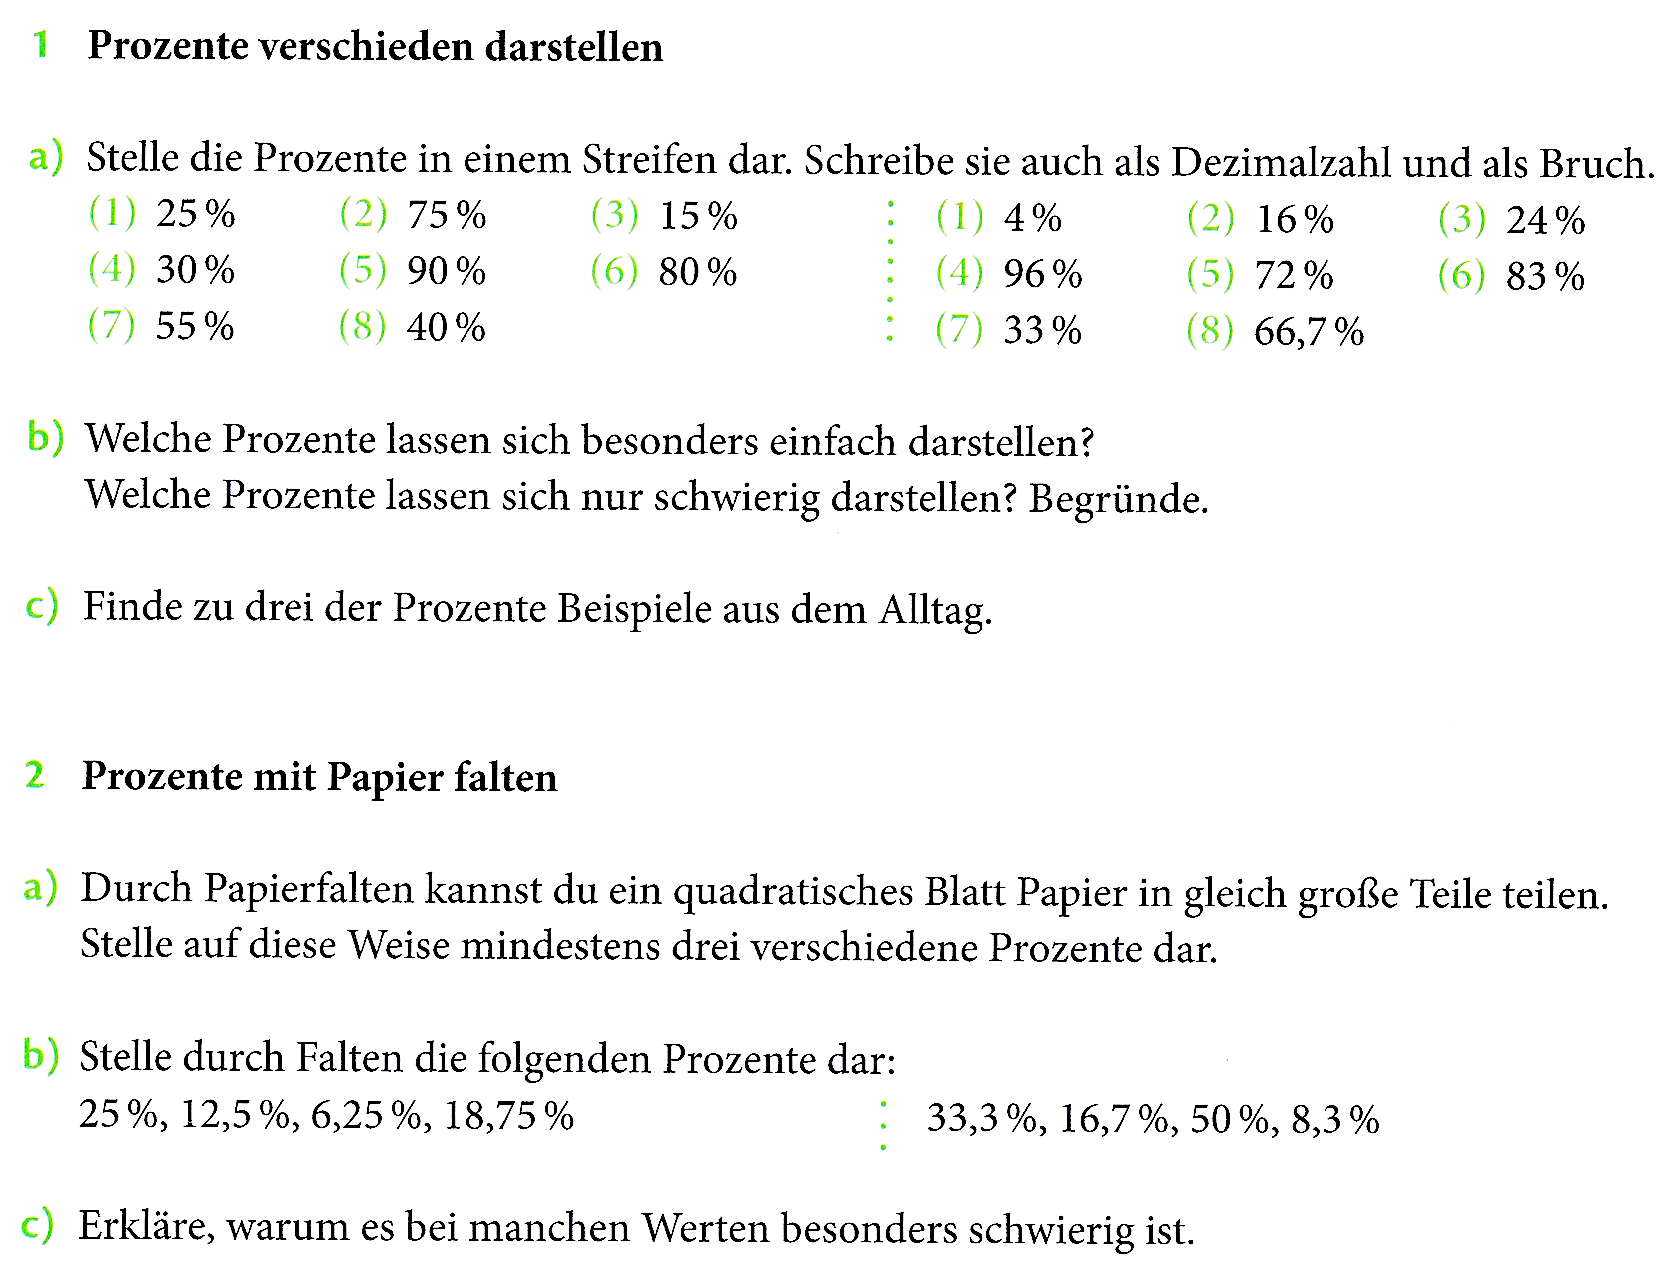
\includegraphics[width=0.75\linewidth]{pictures/10-ProzentUeben} 

    }

    \caption{Übungsaufgaben zur Prozentrechnung (\protect\hyperlink{ref-Barzel2015a}{Leuders et al., 2015, S. 232})}\label{fig:ProzentUeben}
    \end{figure}
\item
  Das \textbf{Vertiefen}, \textbf{Strukturieren} und \textbf{Vernetzen} stärkt das Kompetenzerleben der Schülerinnen und Schüler. Die Aufgaben werden wieder offener und können mit anderen Lerngegenständen in Bezug gebracht werden. Auch können Sonder- oder Grenzfälle der bisher betrachteten Aufgaben nun verstärkt eine Rolle spielen (siehe Abbildung \ref{fig:ProzentVertiefen}).

  \begin{figure}

    {\centering 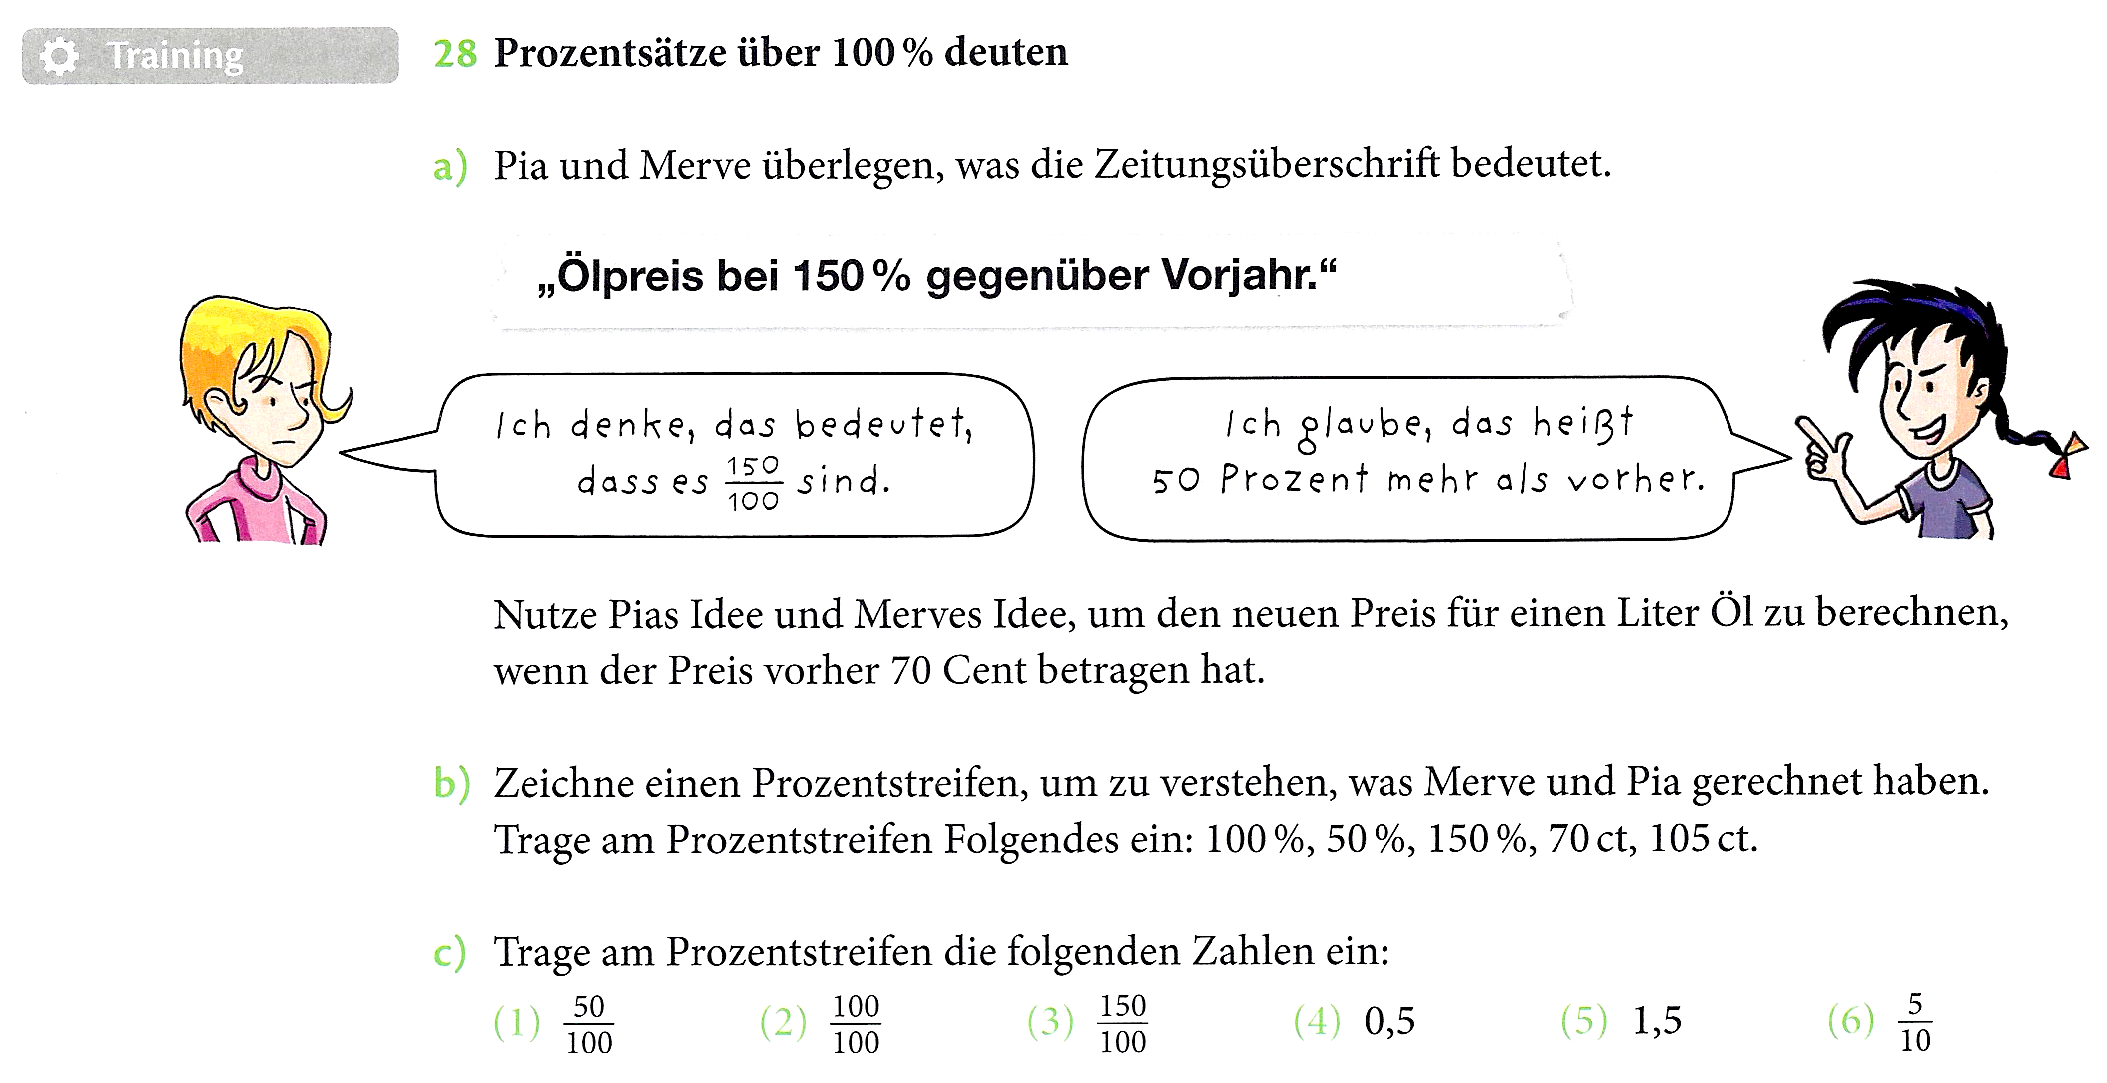
\includegraphics[width=0.75\linewidth]{pictures/10-ProzentVertiefen} 

    }

    \caption{Vertiefungsaufgabe zur Prozentrechnung (\protect\hyperlink{ref-Barzel2015a}{Leuders et al., 2015, S. 241})}\label{fig:ProzentVertiefen}
    \end{figure}
\item
  Die bisher genannten Funktionen hängen oftmals eng mit entsprechenden Unterrichtsphasen zusammen. Davon unabhängig können Aufgaben auch die Funktion des \textbf{Differenzierens} haben. Maßnahmen dafür werden in Abschnitt \ref{differenzieren} näher erläutert.
\item
  Weiterhin ist zwischen \textbf{Lernaufgaben} und \textbf{Leistungsaufgaben} zu unterscheiden. Letztere spielen bei der \textbf{Selbsteinschätzung}, \textbf{Diagnose} und \textbf{Leistungsmessung} eine besondere Rolle (siehe Abbildung \ref{fig:ProzentLeisten}). Insbesondere für solche Aufgaben sollten Operatoren genutzt werden, um die gewünschten Komptenzen gezielt überprüfen zu können, Erwartungen an die Schülerinnen und Schüler transparent zu machen und eine Vergleichbarkeit zu sichern.

  \begin{figure}

    {\centering 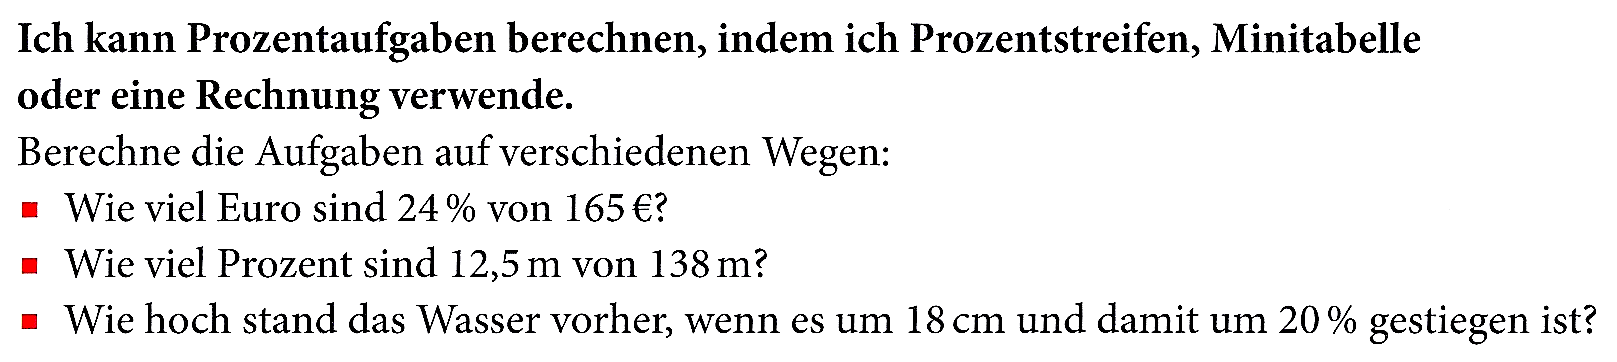
\includegraphics[width=0.75\linewidth]{pictures/10-ProzentLeisten} 

    }

    \caption{Selbsteinschätzungsaufgabe zur Prozentrechnung (\protect\hyperlink{ref-Barzel2015a}{Leuders et al., 2015, S. 244})}\label{fig:ProzentLeisten}
    \end{figure}
\end{itemize}

\hypertarget{produktives-uxfcben}{%
\section{Produktives Üben}\label{produktives-uxfcben}}

\hypertarget{Faehigkeitsaspekte}{%
\subsection{Fähigkeitsaspekte}\label{Faehigkeitsaspekte}}

Nicht selten wird man in Schulbüchern mit sogenannten \emph{Aufgabenplantagen} konfrontiert, also einer Vielzahl an Aufgaben immer derselben Art. Diese haben in der Regel das (berechtigte) Ziel, dass bestimmte Rechenoperation durch wiederholtes Üben automatisiert durchgeführt werden können. Im Schulalltag besteht jedoch die Gefahr, dass das Üben im Mathematikunterricht dann zum alleinigen \emph{Päckchenrechnen} verkommt, was der Vielzahl an \textbf{Fähigkeitsaspekten}, die ausgeprägt werden sollen, nicht gerecht wird.

Diese Fähigkeitsaspekte sind nach \protect\hyperlink{ref-Leuders2009}{Leuders} (\protect\hyperlink{ref-Leuders2009}{2009, S. 133}):

\begin{itemize}
\tightlist
\item
  \textbf{Kenntnisse}, es kann z.~B. die Definition eines math. Inhalts mit eigenen Worten wiedergegeben werden.
\item
  \textbf{Fertigkeiten}, es können z.~B. bestimmte Rechenoperationen durchgeführt werden.
\item
  \textbf{Verstehen/Vorstellungen}, es kann z.~B. an einem Bild der entsprechende math. Inhalt erklärt werden.
\item
  \textbf{Anwendungsfähigkeit}, es können z.~B. unbekannte Situationen mithilfe des math. Inhalts gelöst werden.
\item
  \textbf{(übergreifende) Strategien}, es können z.~B. Heurismen (vgl. \protect\hyperlink{ref-Kuzle}{Kuzle, o.~J.}) mithilfe des math. Inhalts angewandt werden.
\item
  \textbf{Reflexionsfähigkeit}, es kann z.~B. beurteilt werden, inwieweit der math. Inhalt in einer Situation relevant ist.
\item
  \textbf{Einstellungen}, es besteht z.~B. die Bereitschaft, sich mit dem math. Inhalt auseinanderzusetzen.
\end{itemize}

Diese Fähigkeitsaspekte sind nicht als Stufen aufzufassen, sondern gleichermaßen und unabhängig voneinander bedeutsam (\protect\hyperlink{ref-Leuders2009}{Leuders, 2009, S. 133}).

\hypertarget{aufgaben-veruxe4ndern}{%
\subsection{Aufgaben verändern}\label{aufgaben-veruxe4ndern}}

Einerseits sollten Sie als Lehrkraft in der Lage sein, zielgerichtet je nach Fähigkeitsaspekt Aufgaben auszuwählen. Andererseits, und das ist dann notwendig, wenn Sie keine guten Aufgaben finden, müssten Sie auch selbst welche entwickeln können -- was jedoch sehr zeitaufwendig ist. Ein in der Unterrichtspraxis effektiver Umgang ist das Verändern von existierenden Aufgaben, um diese \emph{produktiver} zu machen, d.~h. vielfältige Fähigkeitsaspekte anzusprechen.

\protect\hyperlink{ref-Leuders2009}{Leuders} (\protect\hyperlink{ref-Leuders2009}{2009, S. 137~ff.}) stellt in einer ausführlichen Tabelle (am Beispiel des arithmetischen Mittels) dar, wie man sich ausgehend vom gewünschten Fähigkeitsaspekt (z.~B. »Strukturen reflektieren«) und damit zusammenhängenden Aufgabentypen (z.~B. »Muster erkennen und erzeugen«) an geeigneten Fragetypen (z.~B.»Muster fortsetzen«) orientieren kann, um einen produktiven Umgang mit Aufgaben zu ermöglichen. Mit diesem Hintergrundwissen können Sie Ihren Blick auf existierende Schulbuchaufgaben richten und diese dann zielgerichtet anpassen.

Die soll am Beispiel einer Schulbuchseite zur Prozentrechnung dargestellt werden, siehe Abbildung \ref{fig:ProzentSchulbuch}.



\begin{figure}

{\centering 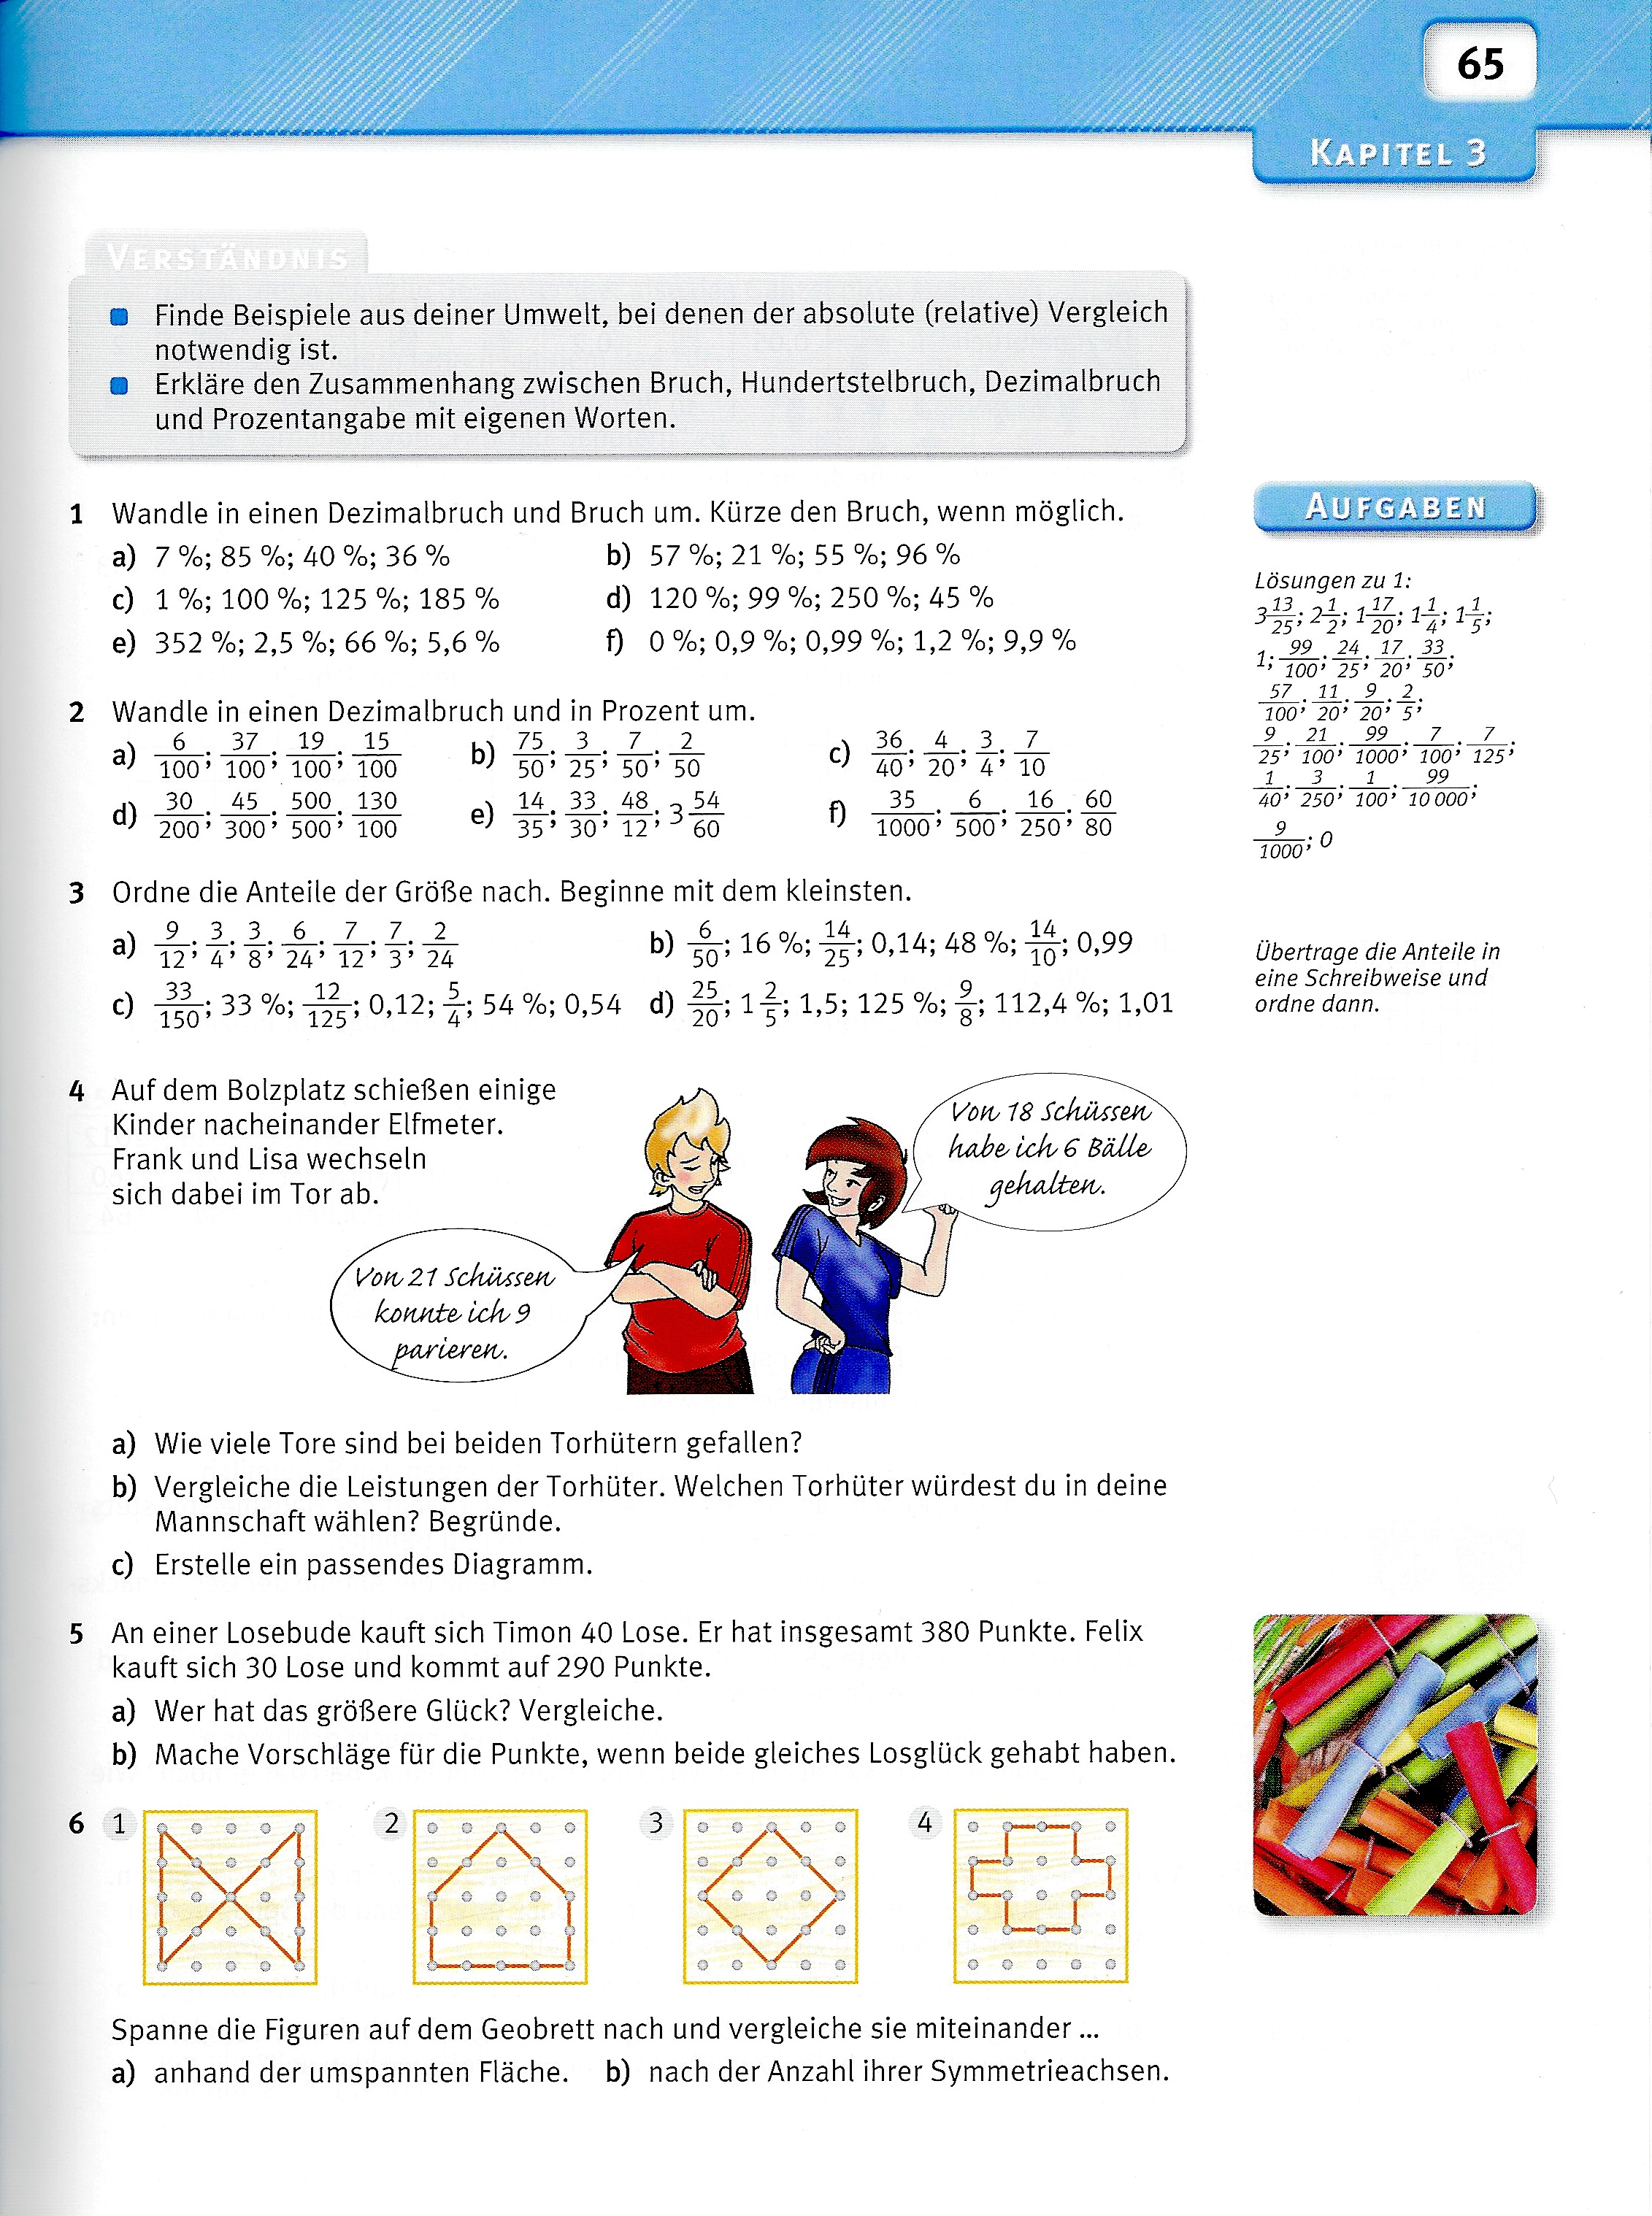
\includegraphics[width=0.75\linewidth]{pictures/10-ProzentSchulbuch} 

}

\caption{Schulbuchseite zur Prozentrechnung (\protect\hyperlink{ref-Kleine2011a}{Kleine \& Ludwig, 2011, S. 65})}\label{fig:ProzentSchulbuch}
\end{figure}

\begin{itemize}
\item
  Bei Aufgabe 2 könnte ergänzt werden:

  \emph{Welche Brüche lassen sich besonders leicht, welche schwerer in Dezimalbrüche und Prozent umrechnen? Woran liegt das?}

  Damit soll die Reflexion darüber angeregt werden, dass das Erweitern und Kürzen, sodass der Nenner 100 ergibt, je nach gegebenem Nenner unterschiedlich schwer sein kann. Hinsichtlich der Tabelle von \protect\hyperlink{ref-Leuders2009}{Leuders} (\protect\hyperlink{ref-Leuders2009}{2009, S. 138}) kann diese Aufgabe der Situation »Strukturen reflektieren« → »Strukturieren« → »Bewerten« zugeordnet werden. Statt alle Päckchen rechnen zu müssen, könnte nach der obigen Reflexion auch aufgefodert werden:

  \emph{Wähle eine leichte und eine schwere Teilaufgabe aus und löse sie.}
\item
  Aufgabe 3 ließe sich ergänzen durch:

  \emph{Wie ändert sich Lisas Leistung, wenn du weitere Schüsse aufs Tor zielst, die sie alle hält?}

  Diese Aufgabe betont den Zusammenhang zwischen Grundwert, Prozentwert und Protenzsatz, da jeder weitere Schuss sowohl den Grundwert als auch Prozentwert um 1 erhöht, womit zwar der Prozentsatz zunimmt, aber nicht linear steigt. Damit kann gleichzeitig eine tiefere Beschäftigung mit der dahinterliegenden arithmetischen Struktur angeregt werden. Nach \protect\hyperlink{ref-Leuders2009}{Leuders} (\protect\hyperlink{ref-Leuders2009}{2009, S. 137}) gehört diese Aufgabe zum Bereich »Probleme lösen« → »Operatives Durcharbeiten« → »Funktionale Abhängigkeit«.
\item
  Aufgabe 5 könnte ergänzt werden:

  \emph{Erfinde eine andere Situation, in der auf dieselbe Art und Weise gerechnet werden kann. Welche deiner Größen entsprechen den »Punkten« und der »Anzahl der Lose« und welche Rolle spielen diese Größen bei der Berechnung?}

  Hierüber wird eine strukturgleiche Übertragung der gegebenen Situation auf eine neue Situation gefordert. Dies führt dazu, sich tiefer mit dem Zusammenhang aus Rechenoperation und Anwendungskontext auseinanderzusetzen und entspricht bei \protect\hyperlink{ref-Leuders2009}{Leuders} (\protect\hyperlink{ref-Leuders2009}{2009, S. 139}) der Kategorie »Anwendungen erkunden« → »Anwenden« → »Anwendungen erfinden«.
\end{itemize}

\hypertarget{differenzieren}{%
\section{Differenzieren}\label{differenzieren}}

Um differenzierenden Unterricht zu ermöglichen, können Aufgaben entsprechend gestaltet werden. Dies kann mit \emph{leichten} und \emph{schweren} Aufgaben erfolgen -- es gibt aber noch weitaus mehr Möglichkeiten. Davon sollen hier einige exemplarisch vorgestellt werden, genauere Maßnahmen finden sich in den jeweils zitierten Quellen.

\hypertarget{gestufte-hilfen}{%
\subsection{Gestufte Hilfen}\label{gestufte-hilfen}}

Bei komplexen Aufgaben bietet es sich an, den Schülerinnen und Schülern gestufte Hilfen bereitzustellen, damit diese im Lösungsweg individuell unterstützt werden können (siehe auch \protect\hyperlink{ref-Zech1998}{Zech, 1998, S. 315~ff.}). Auch wenn Motivationshilfen (\emph{Die Aufgabe ist nicht so schwer.}), Rückmeldungshilfen (\emph{Du bist auf einem guten Weg.}) oder allgemeine strategische Hilfen (\emph{Lies die Aufgabe noch mal durch.}) deratige Unterstützungen sind, sollte bei der stoffdidaktisch-orientierten Unterrichtsplanung der Schwerpunkt auf \textbf{inhaltsorientierten strategischen Hilfen} sowie auf \textbf{inhaltlichen Hilfen} im Zusammenhang mit dem Lerngegenstand liegen.

\begin{itemize}
\item
  Inhaltsorientierte strategische Hilfen beziehen sich auf typische am Lerngegenstand orientierte Herangehensweisen zur Lösung einer Aufgabe. Mögliche Beispiele sind:

  \emph{Veranschauliche dir die Situation mit einer Skizze.}\\
  \emph{Stelle eine Gleichung auf.}\\
  \emph{Orientiere dich beim Vorgehen an dem Beispiel, das du bereits gerechnet hast.}
\item
  Inhaltliche Hilfen beziehen sich direkt auf die mit der Aufgabe verbundenen Begriffe, Regeln und Zusammenhänge. Dies können z.~B. sein:

  \emph{Überlege, was mit dem Flächeninhalt passiert, wenn du die Seitenlängen verdoppelst.}\\
  \emph{Du kannst hier das Kommutativgesetz anwenden.}
\end{itemize}

\protect\hyperlink{ref-Zech1998}{Zech} (\protect\hyperlink{ref-Zech1998}{1998, S. 315}) betont, »nie mehr {[}zu{]} helfen als erforderlich«, um eine Aufgabe erfolgreich lösen zu können. Gestufte Hilfen haben demnach die Funktion, trotz ggf. vorhandener Schwierigkeiten Erfolgserlebnisse bei den Schülerinnen und Schülern zu ermöglichen.

\hypertarget{differenzierende-aufgaben}{%
\subsection{Differenzierende Aufgaben}\label{differenzierende-aufgaben}}

\hypertarget{schwierigkeitsbestimmende-merkmale}{%
\subsubsection{Schwierigkeitsbestimmende Merkmale}\label{schwierigkeitsbestimmende-merkmale}}

Ob eine Aufgabe leicht oder schwer ist, wird natürlich stets subjektiv beeinflusst. Dennoch können schwierigkeitsbestimmende Merkmale von Aufgaben identifiziert werden, die bspw. bei der Konstruktion differenzierender Aufgaben hilfreich sind. Nach \protect\hyperlink{ref-Druke-Noe2018}{Drüke-Noe} (\protect\hyperlink{ref-Druke-Noe2018}{2018, S. 11}) sind diese Merkmale:

\begin{itemize}
\tightlist
\item
  Zugehörigkeit zu einer curricularen Wissensstufe
\item
  Komplexität und Qualität einer erforderlichen Modellierung
\item
  Offenheit des Modellierungsprozesses
\item
  Art des Kontextes
\item
  Erfordernis, mathematische Argumente zu formulieren
\item
  Anzahl zu steuernder Denkprozesse
\item
  Technische Komplexität
\item
  „Umfang`` eines Verarbeitungsprozesses (u.~a. Anzahl der Rechenschritte, Art des Zahlenmaterials)
\item
  Sprachlogische Komplexität
\end{itemize}

Abbildung \ref{fig:Schwierig} zeigt eine mögliche Realisierung zur Generierung unterschiedlich schwerer Aufgaben.



\begin{figure}

{\centering \includegraphics[width=0.75\linewidth]{pictures/10-Schwierig} 

}

\caption{Unterschiedlich schwere Aufgaben zum Prismenvolument (aus \protect\hyperlink{ref-Druke-Noe2018}{Drüke-Noe, 2018, S. 10})}\label{fig:Schwierig}
\end{figure}

In der Unterrichtspraxis kann dies nun bedeuten, dass Sie auswählen, welche Schülerinnen und Schüler welche Aufgaben lösen (sogenannte \textbf{paralleldifferenzierende Aufgaben}, vgl. \protect\hyperlink{ref-Leuders2015}{Leuders, 2015, S. 441}), Sie können die Auswahl den Lernenden selbst überlassen oder auch eine Stufung im Schwierigkeitsgrad vornehmen, die dann durchlaufen werden soll (\textbf{gestuft differenzierende Aufgaben}).

\hypertarget{bluxfctenaufgaben}{%
\subsubsection{Blütenaufgaben}\label{bluxfctenaufgaben}}

Eine besondere Form gestufter Aufgaben sind \textbf{Blütenaufgaben}. Diese sind dadurch gekennzeichnet, dass der \textbf{Offenheitscharakter der Teilaufgaben steigt}, wobei alle Teilaufgaben einem \textbf{gemeinsamen Kontext} zuzuordnen sind. Die Schülerinnen und Schüler entscheiden dabei selbst, wie weit sie in der Bearbeitung der Aufgabe vordringen, womit Blütenaufgaben \emph{anforderungsgestuft} und \emph{selbstdifferenzierend} sind (vgl. \protect\hyperlink{ref-Bruder2015a}{Bruder et al., 2015, S. 528~f.}).

Einen etwas ausführlicheren Hintergrund und einige Beispiele zeigt ein Video von \protect\hyperlink{ref-Quarder2020}{Quarder} (\protect\hyperlink{ref-Quarder2020}{2020}).

\hypertarget{natuxfcrliche-differenzierung}{%
\subsection{Natürliche Differenzierung}\label{natuxfcrliche-differenzierung}}

Eine noch offenere und für die Unterrichtsplanung durchaus anspruchsvollere Form ist die \textbf{natürliche Differenzierung}. Nach \protect\hyperlink{ref-Krauthausen2010}{Krauthausen \& Scherer} (\protect\hyperlink{ref-Krauthausen2010}{2010, S. 5~f.}) weist eine natürlich differenzierte Lernumgebung folgende Merkmale auf:

\begin{itemize}
\item
  Alle Schülerinnen und Schüler arbeiten an einem gemeinsamen Lerngegenstand mit \textbf{demselben Lernangebot}, d.~h. allen wird dasselbe Material zur Verfügung gestellt.
\item
  Das Material weist eine \textbf{inhaltliche Ganzheitlichkeit} auf, d.~h. es ist komplex genug, um sich tiefgründig mit dem Lerngegenstand auseinandersetzen zu können.
\item
  Es erfolgt (durch die Lehrkraft) eine \textbf{fachliche Rahmung}, die naturgemäß zu \textbf{Fragestellungen unterschiedlichen Schwierigkeitsgrades} führt. Daraufhin haben die Schülerinnen und Schüler die \textbf{Wahl, auf welchem Nivau} die Problemstellung betrachtet wird -- das Material muss hier also verschiedene Niveaus gleichermaßen ermöglichen.
\item
  Den Schülerinnen und Schülern ist es \textbf{freigestellt, welche Wege, Hilfsmittel und Darstellungsweisen} genutzt werden, um die Problemstellung zu bearbeiten. Die Lehrkraft hat hier die Veranwortung, die Schülerinnen und Schüler zu \emph{befähigen}, eine sinnvolle Auswahl zu treffen. Dies kann bspw. durch geeignete Impulse erfolgen, auch ist ggf. eine explizite Heurismenschulung notwendig.
\item
  Letztlich ist natürliche Differenzierung durch ein intensives \textbf{soziales Mit- und Voneinanderlernen} geprägt, wofür eine kommunikationsfreundliche Umgebung geschaffen werden muss. Dies betrifft z.~B. die Diskussion unterschiedlicher Lösungswege, \emph{natürlich} entstandene (ggf. abweichende) Fragestellungen oder auch unterschiedliche Auffassungen.
\end{itemize}

Bisher existieren wenige Aufgaben zur natürlichen Differenzierung für die Sekundarstufe. Ein Beispiel zur Bruchrechnung zeigen \protect\hyperlink{ref-Fockler2018}{Föckler et al.} (\protect\hyperlink{ref-Fockler2018}{2018, S. 2}).

\hypertarget{aufgaben-gestalten-nachbereitung}{%
\section{Zum Nachbereiten}\label{aufgaben-gestalten-nachbereitung}}

Erstellen Sie zum Lerngegenstand \emph{Rechnen mit negativen Zahlen}

\begin{enumerate}
\def\labelenumi{\alph{enumi})}
\item
  jeweils eine Aufgabe zum Erkunden, Sichern, Üben und Vertiefen,
\item
  für die Vertiefungsaufgabe zwei bis drei gestufte Hilfen, sowie
\item
  eine Blütenaufgabe.
\end{enumerate}

\hypertarget{appendix-anhang}{%
\appendix}


\hypertarget{leitidee-zahl}{%
\chapter{Leitidee Zahl}\label{leitidee-zahl}}

\begin{quote}
\textbf{Bedeutsame Lerngegenstände}

\begin{itemize}
\tightlist
\item
  Zahlbereiche
\item
  Prozente
\item
  Kombinatorik
\item
  Grenzwert
\item
  Tupel, Matrizen
\end{itemize}

\textbf{Literaturempfehlungen}

\begin{itemize}
\tightlist
\item
  \protect\hyperlink{ref-Padberg2015}{Padberg \& Büchter} (\protect\hyperlink{ref-Padberg2015}{2015}): \emph{Einführung Mathematik Primarstufe -- Arithmetik}
\item
  \protect\hyperlink{ref-Padberg:2017}{Padberg \& Wartha} (\protect\hyperlink{ref-Padberg:2017}{2017}): \emph{Didaktik der Bruchrechnung}
\end{itemize}
\end{quote}

\hypertarget{strukturierung-der-leitidee-zahl}{%
\section{Strukturierung der Leitidee}\label{strukturierung-der-leitidee-zahl}}

In den Bildungsstandards für die allgemeine Hochschulreife lautet diese Leitidee »Algorithmus und Zahl« (\protect\hyperlink{ref-KMK:2012}{Sekretariat der Ständigen Konferenz der Kultusminister der Länder in der Bundesrepublik Deutschland, 2012, S. 11}), in denen für den Primarbereich »Zahlen und Operationen« (\protect\hyperlink{ref-KMK2005}{Sekretariat der Ständigen Konferenz der Kultusminister der Länder in der Bundesrepublik Deutschland, 2005, S. 9}).

Das \protect\hyperlink{ref-LISUM2021}{LISUM} (\protect\hyperlink{ref-LISUM2021}{2021}) hat für die Primarstufe und Sekundarstufe I ein Konzeptbild herausgegeben (siehe Abbildung \ref{fig:KonzeptZahl}), ergänzt durch einen didaktischen Kommentar von \protect\hyperlink{ref-Schulz}{Schulz} (\protect\hyperlink{ref-Schulz}{o.~J.}) und Materialien zur Diagnose und Förderung (\protect\hyperlink{ref-LISUMb}{LISUM, o.~J.-g}).



\begin{figure}

{\centering 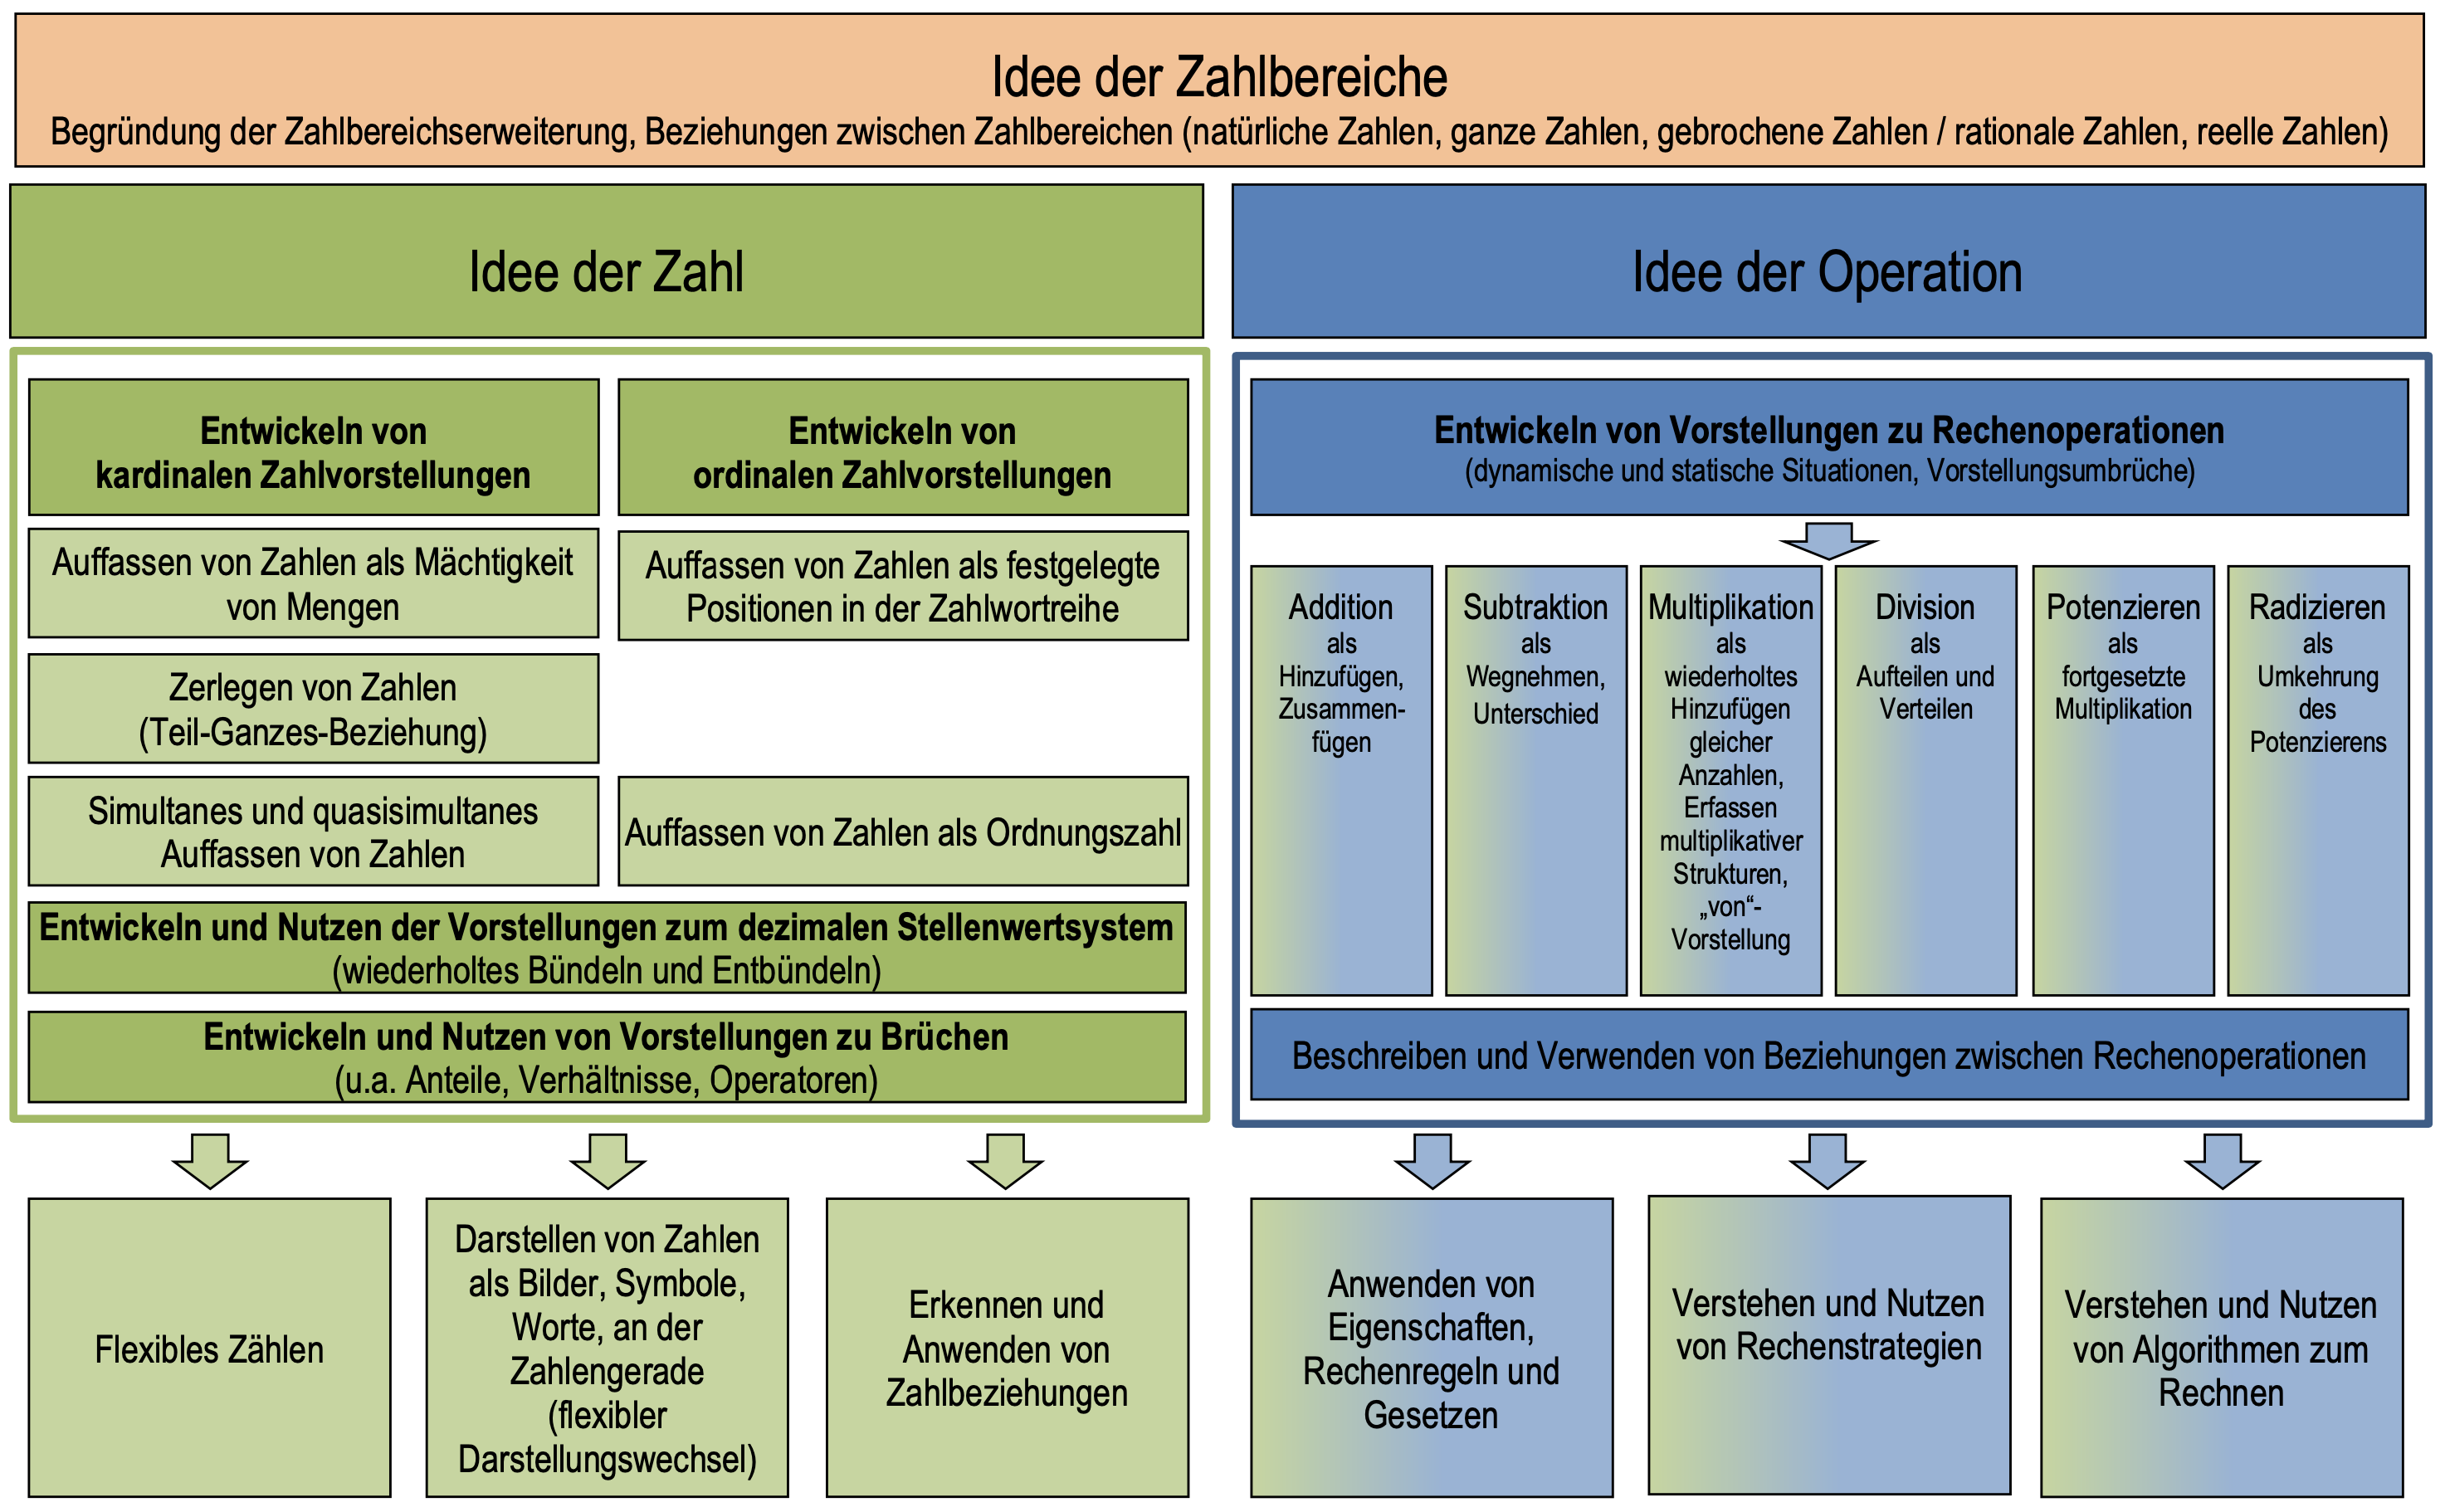
\includegraphics[width=0.9\linewidth]{pictures/A-KonzeptZahl} 

}

\caption{Konzeptbild zur Leitidee \emph{Zahlen und Operationen} (\protect\hyperlink{ref-LISUM2021}{LISUM, 2021})}\label{fig:KonzeptZahl}
\end{figure}

\hypertarget{aufbau-der-zahlbereiche}{%
\section{Aufbau der Zahlbereiche}\label{aufbau-der-zahlbereiche}}

Die Einführung der Zahlbereiche unterscheidet sich deutlich zwischen Schule und Universität. Dies beginnt schon bei der Reihenfolge: Während in der Schule nach den Natürlichen Zahlen i.~d.~R. die Bruchzahlen eingeführt werden, folgt in der Hochschulmathematik normalerweise erst die Einführung der negativen Zahlen.

\begin{figure}

{\centering 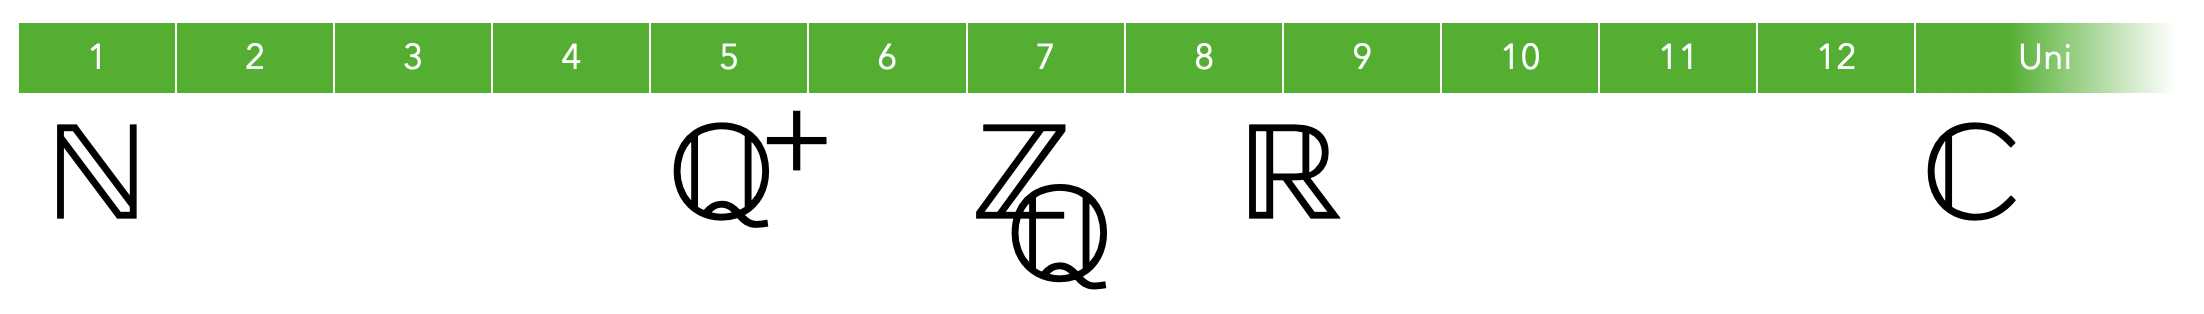
\includegraphics[width=1\linewidth]{pictures/A-ZahlReihenfolge} 

}

\caption{Zahlbereiche im Laufe der Schulzeit}\label{fig:ZahlReihenfolge}
\end{figure}

Aus Abbildung \ref{fig:ZahlReihenfolge} wird weiterhin sichtbar, dass über einen sehr langen Zeitraum ausschließlich mit Natürlichen Zahlen gearbeitet wird, was Vorstellungen verfestigt, die dann ggf. in den weiteren Zahlbereichen nicht mehr tragfähig sind (vgl. Abschnitt \ref{bruchzahlen} und die dortige \protect\hyperlink{fn5}{Fußnote zu Fehlvorstellungen}).

\hypertarget{hochschulperspektive}{%
\subsection{Hochschulperspektive}\label{hochschulperspektive}}

In universitären Veranstaltungen ist als Aufbau der Zahlbereiche üblich:

\begin{enumerate}
\def\labelenumi{\arabic{enumi}.}
\tightlist
\item
  Definition der Natürlichen Zahlen als Ordinalzahlen über die Peano-Axiome.
\item
  Definition der Natürlichen Zahlen als Kardinalzahlen über die Anzahl der Elemente eine Menge. Dabei werden Bijektionen zwischen gleichmächtigen Mengen betrachtet und eine Zahl \(n\) kann als Äquivalenzklasse aufgefasst werden, die für alle Mengen der entsprechenden Mächtigkeit steht.
\item
  Definition der Ganzen Zahlen, ebenfalls über Äquivalenzklassen von geordneten Paaren Natürlicher Zahlen, wobei \((n,m)\) und \((k,l)\) in Relation zueinander stehen, wenn \(n+l = k+m\) gilt. Es ist hier notwendig, über die Addition zu definieren (und nicht etwa über die Relation, wenn \(n-m = k-l\) gilt), da die Existenz eines Ergebnisses \(n-m\) ja für \(n,m\in\mathbb{N}\) noch gar nicht gesichert ist.
\item
  Definition der Rationalen Zahlen als Äquivalenzklassen von geordneten Paaren Ganzer Zahlen, wobei \((r,s)\) und \((u,v)\) in Relation zueinander stehen, wenn \(r\cdot v = s\cdot u\) gilt. Zu Beachten ist, dass als zweiter Eintrag der Paare \(0\) ausgeschlossen wird.
\item
  Definition der Reellen Zahlen als Äquivalenzklassen von Cauchy-Folgen, die in Relation zueinander stehen, wenn ihre Differenz eine Nullfolge ist (also sie denselben Grenzwert haben). Auch hier ist der \emph{Umweg} über die Nullfolgen notwendig, da die Existenz des Grenzwertes in den Rationalen Zahlen nicht gesichert ist -- es werden ja damit erst die Reellen Zahlen konstruiert.
\item
  Definition der Komplexen Zahlen als Paare Reeller Zahlen.
\end{enumerate}

Bei all den Zahlbereichserweiterungen muss stets überprüft werden, ob diese \emph{wohldefiniert} sind, also die Rechengesetze im bisherigen Zahlbereich auf den neuen übertragbar sind und dies zu keinen Widersprüchen führt.

\hypertarget{schulperspektive}{%
\subsection{Schulperspektive}\label{schulperspektive}}

Auch wenn im Matheamtikunterricht keine Peano-Axiome, Äquivalenzklassen oder Cauchy-Folgen betrachtet werden, werden bei den Zahlbereichen dennoch Ideen der fachmathematischen Zusammenhänge aufgegriffen und sind für den Lernfortschritt bedeutsam.

\begin{itemize}
\item
  Die kardinale Vorstellung \textbf{Natürlicher Zahlen} wird in der Grundschule unterstützt, indem eine bestimmte Anzahl an Objekten eingekreist werden muss und Mengen strukturiert erfasst werden (vgl. \protect\hyperlink{ref-DZLM}{DZLM, o.~J.}).
\item
  Die Einführung \textbf{Ganzer Zahlen} über Paare Natürlicher Zahlen kann im Unterricht über sogenannte Guthaben-Schulen-Situationen besprochen werden. Dabei werden bspw. Guthaben- und Schulkarten gesammelt und untersucht, wer denselben \emph{Kontostand} hat. Daran können auch einige der Rechengesetze erarbeitet werden (siehe z.~B. \protect\hyperlink{ref-Hattermann2014}{Hattermann et al., 2014}).
\item
  Die Idee der Äquivalenzklassen spielt bei \textbf{Rationalen Zahlen} eine Rolle, wenn besprochen wird, dass verschiedene Repräsentanten (wie z.~B. \(\frac{2}{3}\) und \(\frac{4}{6}\)) für dieselbe Zahl stehen können.
\item
  \textbf{Reelle Zahlen} können in der Schule über Intervallschachtelungen angenähert werden, was die Idee der konvergierenden Cauchy-Folgen aufgreift. Der Fokus liegt dabei jedoch weniger in der Nichtexistenz des Grenzwertes in \(\mathbb{Q}\), sondern vielmehr in der Möglichkeit, bestimmte Zahlen (z.~B. \(\sqrt{2}\)) als Rationale Zahl darzustellen.
\end{itemize}

\hypertarget{leitidee-messen}{%
\chapter{Leitidee Messen}\label{leitidee-messen}}

\begin{quote}
\textbf{Bedeutsame Lerngegenstände}

\begin{itemize}
\tightlist
\item
  Größen
\item
  Flächeninhalt
\item
  Volumen
\item
  Anstieg/Steigung
\item
  Erwartungswert
\item
  Standardabweichung
\end{itemize}
\end{quote}

\hypertarget{strukturierung-der-leitidee-messen}{%
\section{Strukturierung der Leitidee}\label{strukturierung-der-leitidee-messen}}

In den Bildungsstandards für den Primarbereich lautet diese Leitidee »Größen und Messen« (\protect\hyperlink{ref-KMK2005}{Sekretariat der Ständigen Konferenz der Kultusminister der Länder in der Bundesrepublik Deutschland, 2005, S. 11}).

Das \protect\hyperlink{ref-LISUMf}{LISUM} (\protect\hyperlink{ref-LISUMf}{o.~J.-f}) hat für die Primarstufe und Sekundarstufe I ein Konzeptbild herausgegeben (siehe Abbildung \ref{fig:KonzeptMessen}), ergänzt durch einen didaktischen Kommentar von \protect\hyperlink{ref-Kortenkampb}{Kortenkamp \& Kuzle} (\protect\hyperlink{ref-Kortenkampb}{o.~J.-c}) und Materialien zur Diagnose und Förderung (\protect\hyperlink{ref-LISUMe}{LISUM, o.~J.-e}).



\begin{figure}

{\centering 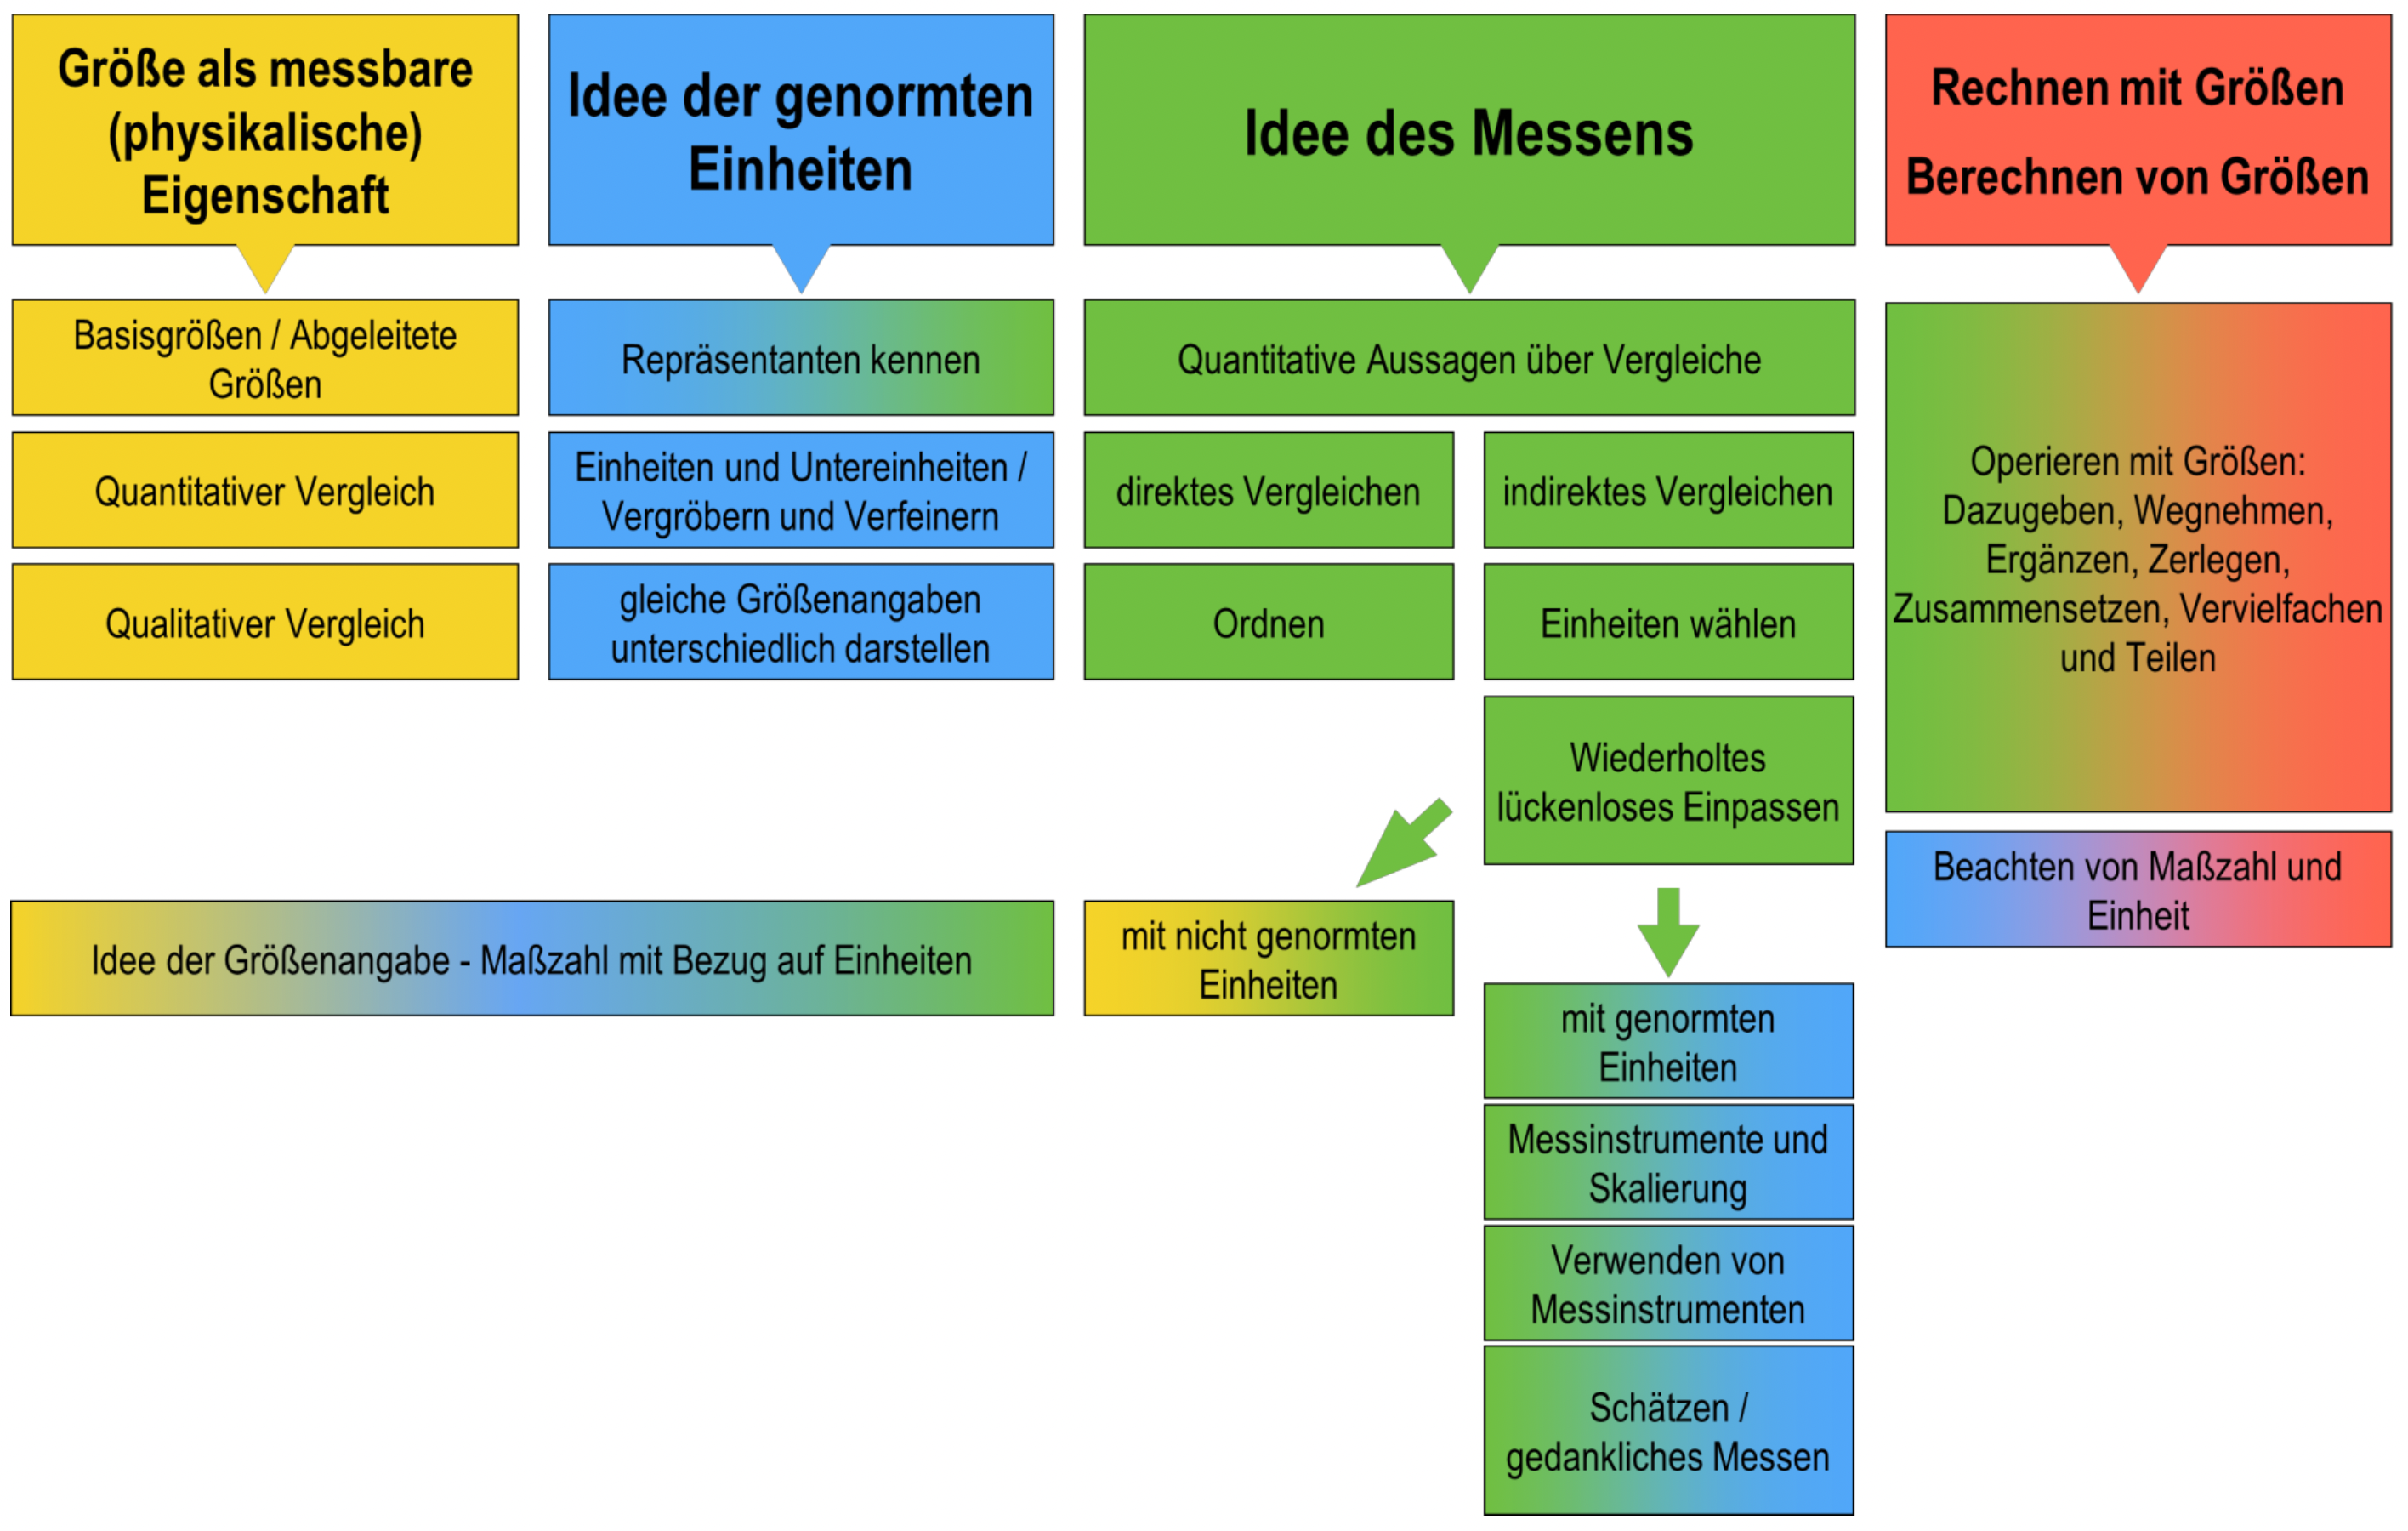
\includegraphics[width=0.9\linewidth]{pictures/B-KonzeptMessen} 

}

\caption{Konzeptbild zur Leitidee \emph{Größen und Messen} (\protect\hyperlink{ref-LISUMf}{LISUM, o.~J.-f})}\label{fig:KonzeptMessen}
\end{figure}

Grundlegende Überlegungen zu der Leitidee finden sich am Beispiel des Flächeninhalts im \protect\hyperlink{erstes-intermezzo-flaecheninhalt}{Ersten Intermezzo}.

\hypertarget{leitidee-raum-und-form}{%
\chapter{Leitidee Raum und Form}\label{leitidee-raum-und-form}}

\begin{quote}
\textbf{Bedeutsame Lerngegenstände}

\begin{itemize}
\tightlist
\item
  Punkt, Strecke
\item
  Dreieck, Viereck
\item
  Winkel
\item
  Geometrische Körper
\item
  Vektor
\item
  Skalarprodukt
\item
  Gerade, Ebene
\item
  Sätze am Kreis
\item
  Satzgruppe des Pythagoras
\end{itemize}

\textbf{Literaturempfehlungen}

\begin{itemize}
\tightlist
\item
  \protect\hyperlink{ref-Franke2016}{Franke \& Reinhold} (\protect\hyperlink{ref-Franke2016}{2016}): \emph{Didaktik der Geometrie. In der Grundschule}
\item
  \protect\hyperlink{ref-Weigand2018}{Weigand et al.} (\protect\hyperlink{ref-Weigand2018}{2018}): \emph{Didaktik der Geometrie für die Sekundarstufe I}
\item
  \protect\hyperlink{ref-Tietze:2000}{Tietze et al.} (\protect\hyperlink{ref-Tietze:2000}{2000b}): \emph{Mathematikunterricht in der Sekundarstufe II. Band 2: Didaktik der Analytischen Geometrie und Linearen Algebra}
\end{itemize}
\end{quote}

\hypertarget{uxfcbersicht-zur-geometrie}{%
\section{Übersicht zur Geometrie}\label{uxfcbersicht-zur-geometrie}}

Im Rahmen der Vorlesung wurde ein Übersichtsbild erstellt, in dem geometrische Objekte (gelb), Relationen (rot), Sätze (blau) und relevante Werkzeuge (grün) in Beziehung zueinander gesetzt werden (siehe Abbildung \ref{fig:KonzeptRaumForm}. Die Übersicht steht auch als \href{files/Stoffdidaktik-WiSe2122-AnhangR-KonzeptRaumForm.pdf}{pdf-Datei} zur Verfügung.

\begin{figure}

{\centering 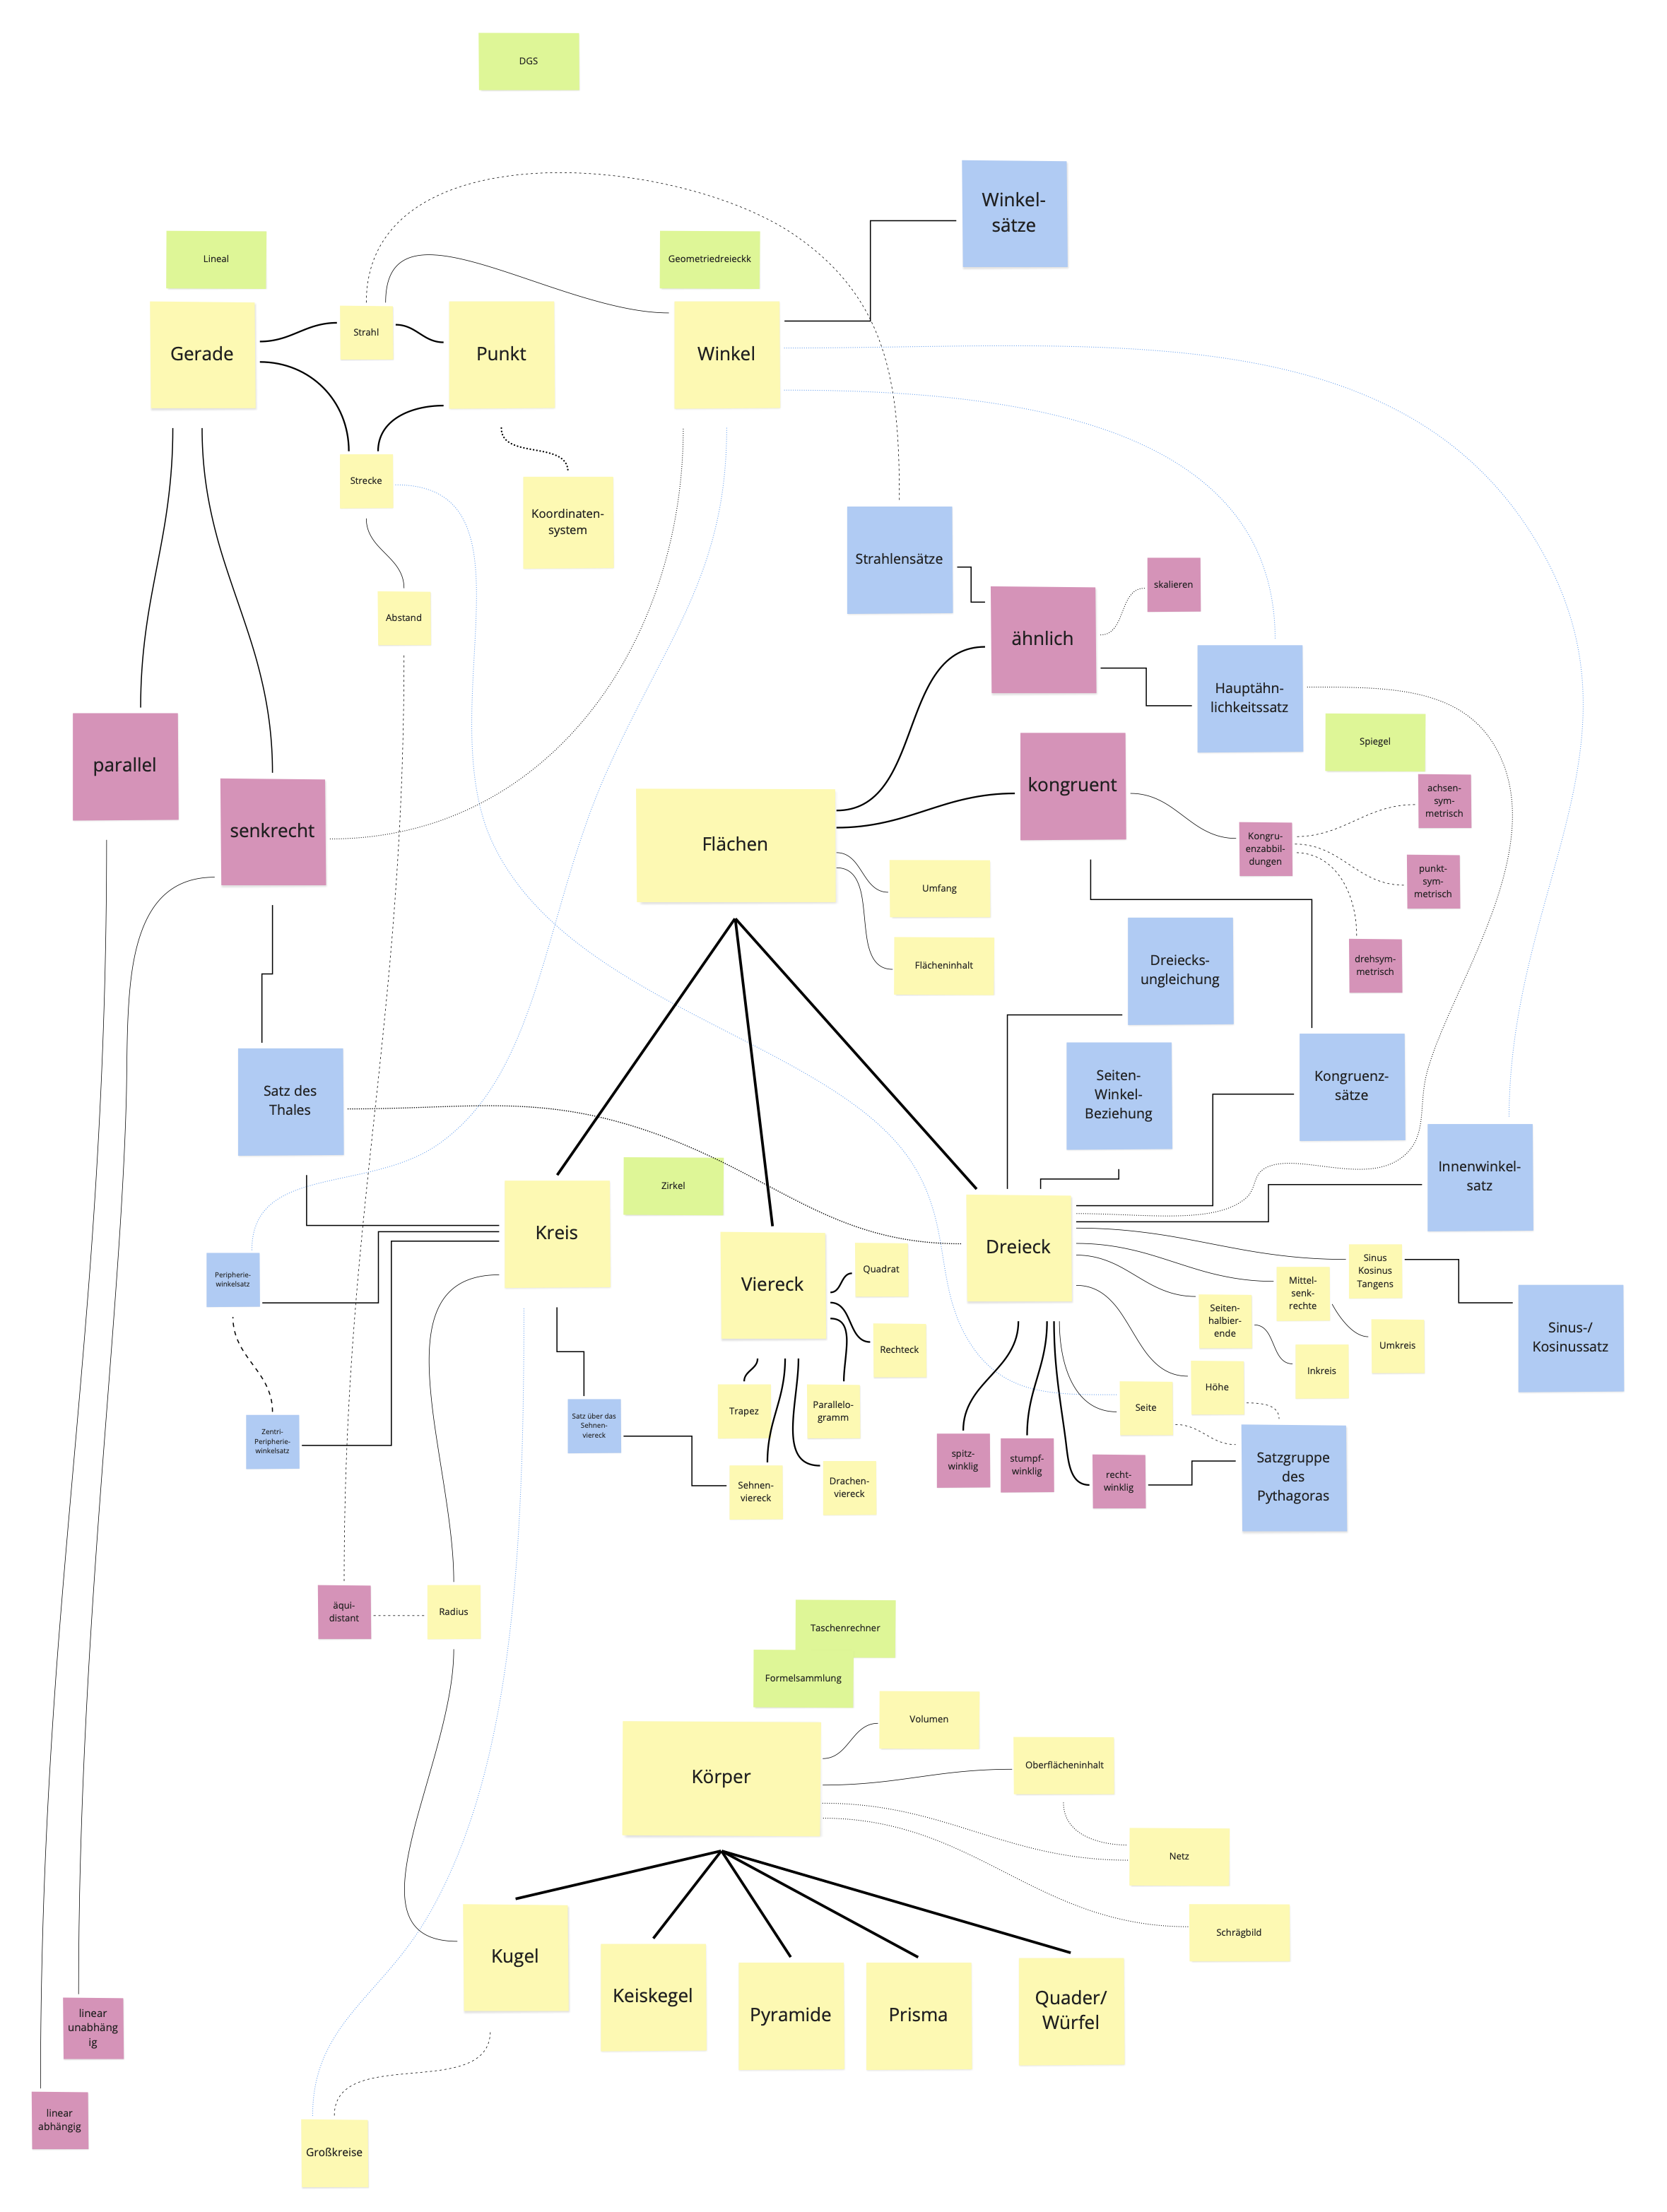
\includegraphics[width=0.75\linewidth]{pictures/D-KonzeptRaumForm} 

}

\caption{Übersicht zur Geometrie}\label{fig:KonzeptRaumForm}
\end{figure}

Eine derartige Übersicht kann Ihnen bei der stoffdidaktischen Analyse helfen, fachliche Zusammenhänge im Blick zu behalten und Sie in der Spezifizierung und Strukturierung von Lerninhalten zu unterstützen.

\hypertarget{elementargeometrische-suxe4tze}{%
\section{Elementargeometrische Sätze}\label{elementargeometrische-suxe4tze}}

Elementargeometrische Sätze bieten eine gute Möglichkeit, Argumentieren und Beweisen auf verschiedenen Niveaus im Mathematikunterricht zu realisieren.

\hypertarget{innenwinkelsatz-fuxfcr-dreiecke}{%
\subsection{Innenwinkelsatz für Dreiecke}\label{innenwinkelsatz-fuxfcr-dreiecke}}

Dass die Innenwinkelsumme von (ebenen) Dreiecken stets \(180°\) beträgt, lässt sich auf verschiedene Weisen plausibel machen und begründen.

Zunächst einmal ist es möglich, die Innenwinkel tatsächlich \textbf{auszumessen und zu addieren}. Dies ist besonders dann überzeugend, wenn die Schülerinnen und Schüler selbst ein beliebiges Dreieck zeichnen und daran ihre Messungen vornehmen. Aufgrund von Messungenauigkeiten wird es ggf. vorkommen, dass die Summe nicht exakt \(180°\) beträgt, aber immerhin sollten sich alle Innenwinkelsummen in diesem Bereich bewegen. Ein nächster Schritt könnte die Nutzung \textbf{Dynamischer Geometriesoftware} sein, wo die Messungen und die Summe exakter bestimmt werden können. Dabei überzeugt weiterhin die Möglichkeit, das Dreieck selbst zu variieren und simultan zu erkennen, dass sich zwar die Größen der drei Innenwinkel ändern, nicht jedoch ihre Summe.

Auf enaktiver Ebene sind das \textbf{Abreißen von Ecken}\footnote{Es ist darauf zu achten, dass wirklich \emph{gerissen} und nicht \emph{geschnitten} wird, weil sonst nicht mehr erkennbar ist, was die eigentliche Ecke war.} oder das \textbf{Aneinanderlegen zueinander kongruenter Dreiecke} mögliche Herangehensweisen, um einen gestreckten Winkel von \(180°\) zu erzeugen (siehe Abbildung \ref{fig:InnenwinkelReissen}).



\begin{figure}

{\centering 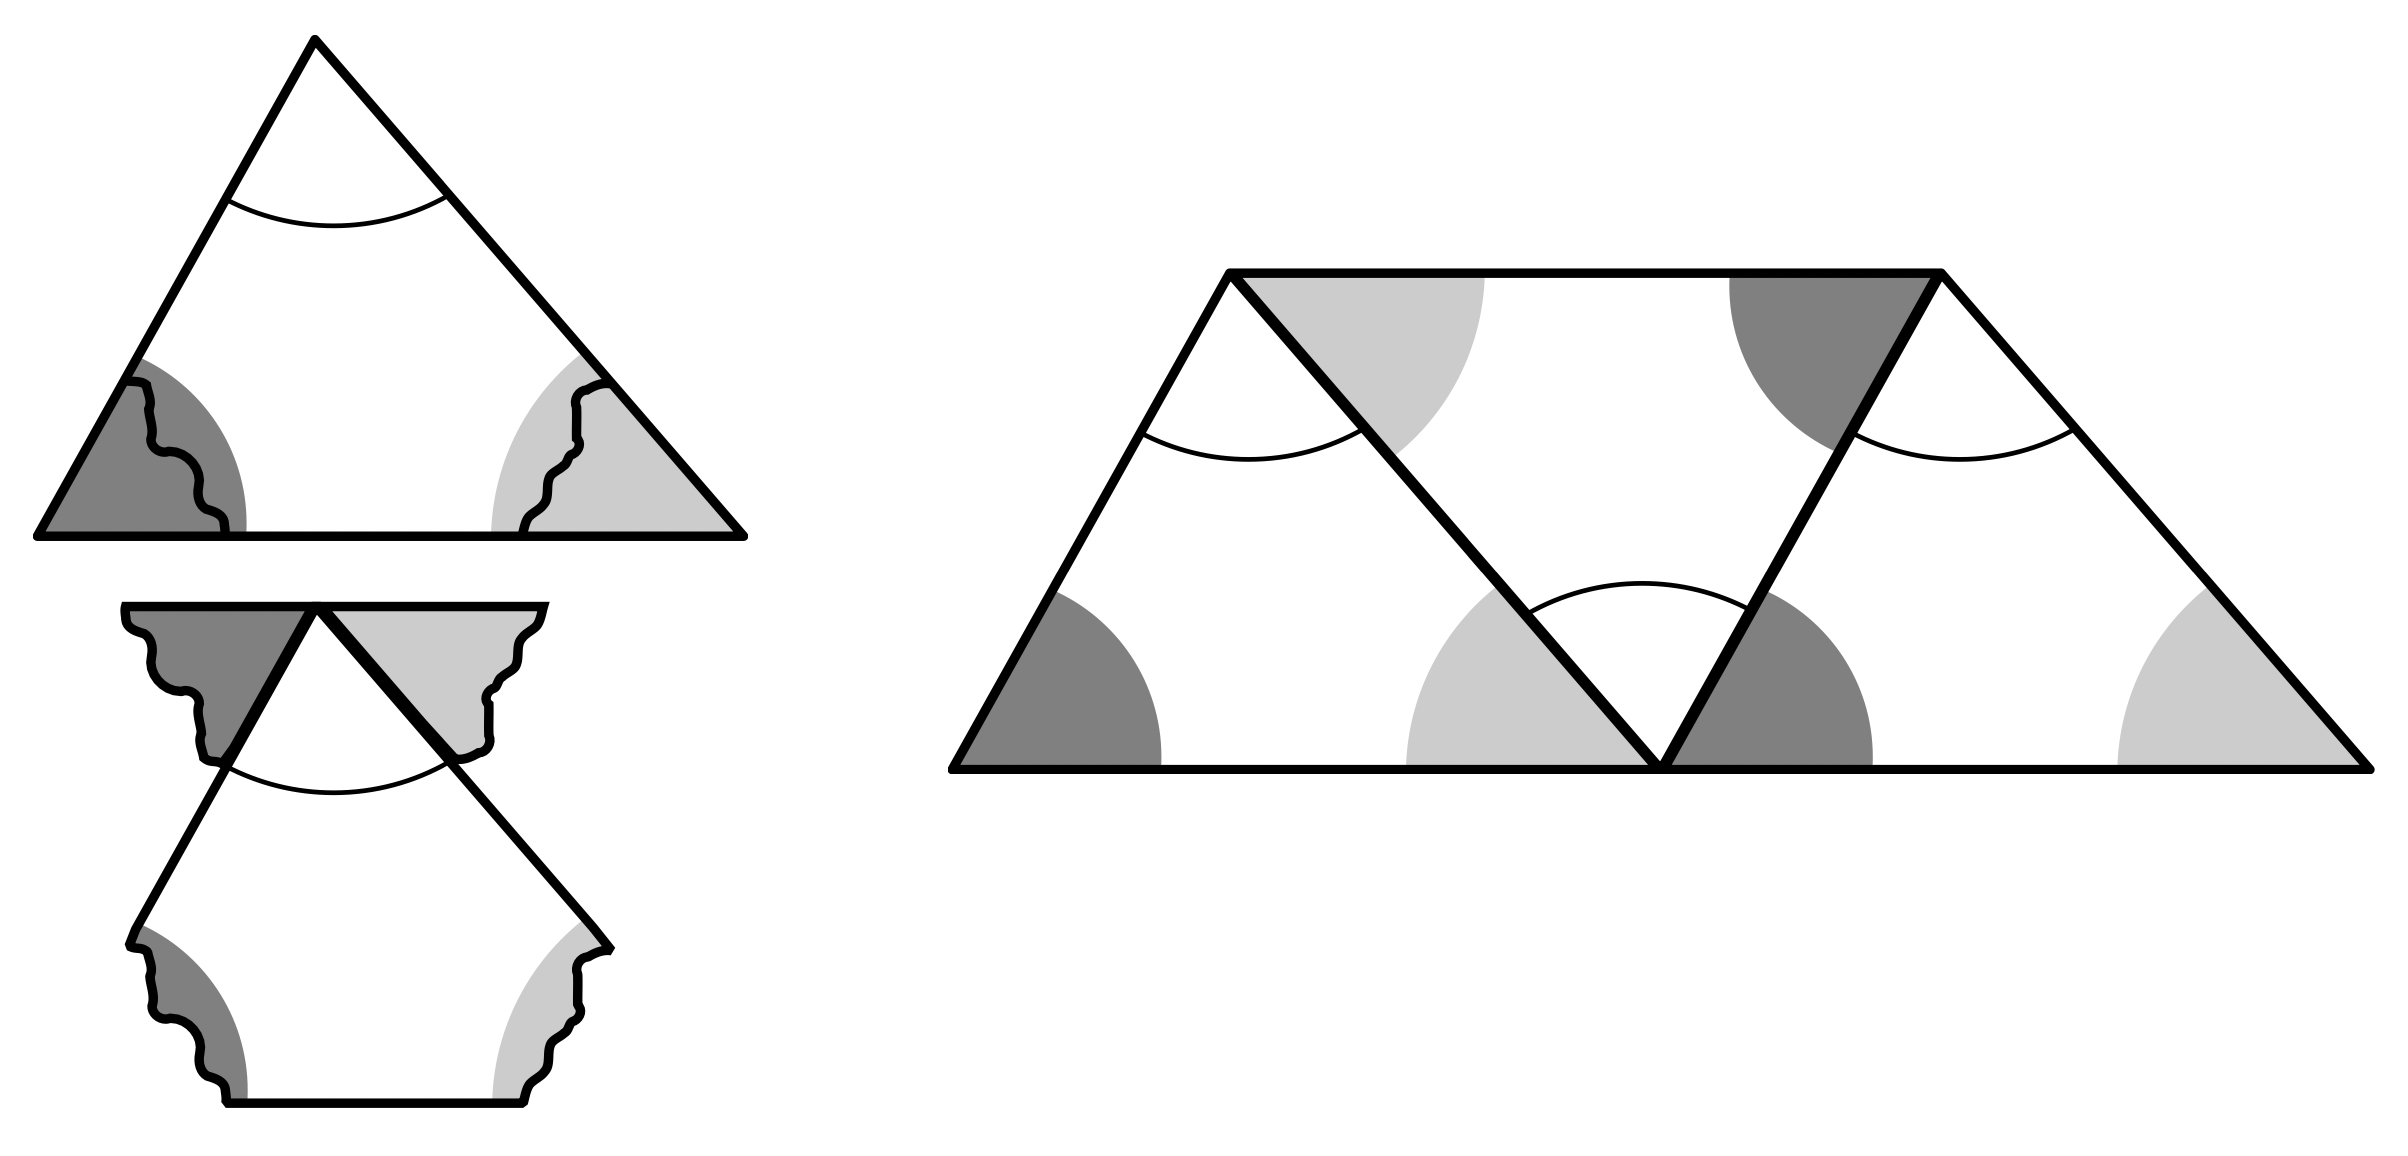
\includegraphics[width=0.75\linewidth]{pictures/C-InnenwinkelReissen} 

}

\caption{Innenwinkelsumme enaktiv bestimmen (\protect\hyperlink{ref-Etzold2014a}{Etzold \& Petzschler, 2014, S. 32})}\label{fig:InnenwinkelReissen}
\end{figure}

Gegenüber dem Messen und Rechnen hat dieses Vorgehen, insbesondere das Aneinanderlegen, die Besonderheit, dass daran schon eine allgemeine Beweisidee sichtbar wird. Dies ist auch der Fall, wenn man einen \textbf{Stift im Inneren des Dreiecks wandern}, der, wenn er alle Ecken einmal abgelaufen ist, insgesamt eine halbe Drehung (also um \(180°\)) vollführt hat (siehe Abbildung \ref{fig:InnenwinkelStift}).

\begin{figure}

{\centering 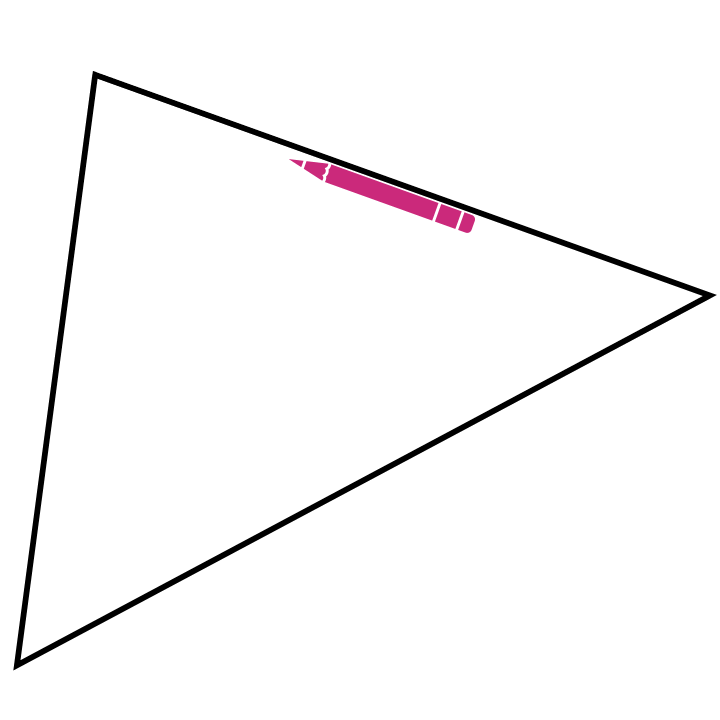
\includegraphics[width=0.5\linewidth]{pictures/C-InnenwinkelStift} 

}

\caption{Innenwinkelsumme mit Stiftbewegung erfahren}\label{fig:InnenwinkelStift}
\end{figure}

Für den eigentlichen Beweis kann man parallel zu einer Dreiecksseite einen Gerade durch den gegenüberliegenden Punkt zeichnen (siehe Abbildung \ref{fig:InnenwinkelBeweisfigure}) und den gestreckten Winkel von \(180°\) mithilfe Wechselwinkelsatzes begründen.

\begin{figure}

{\centering 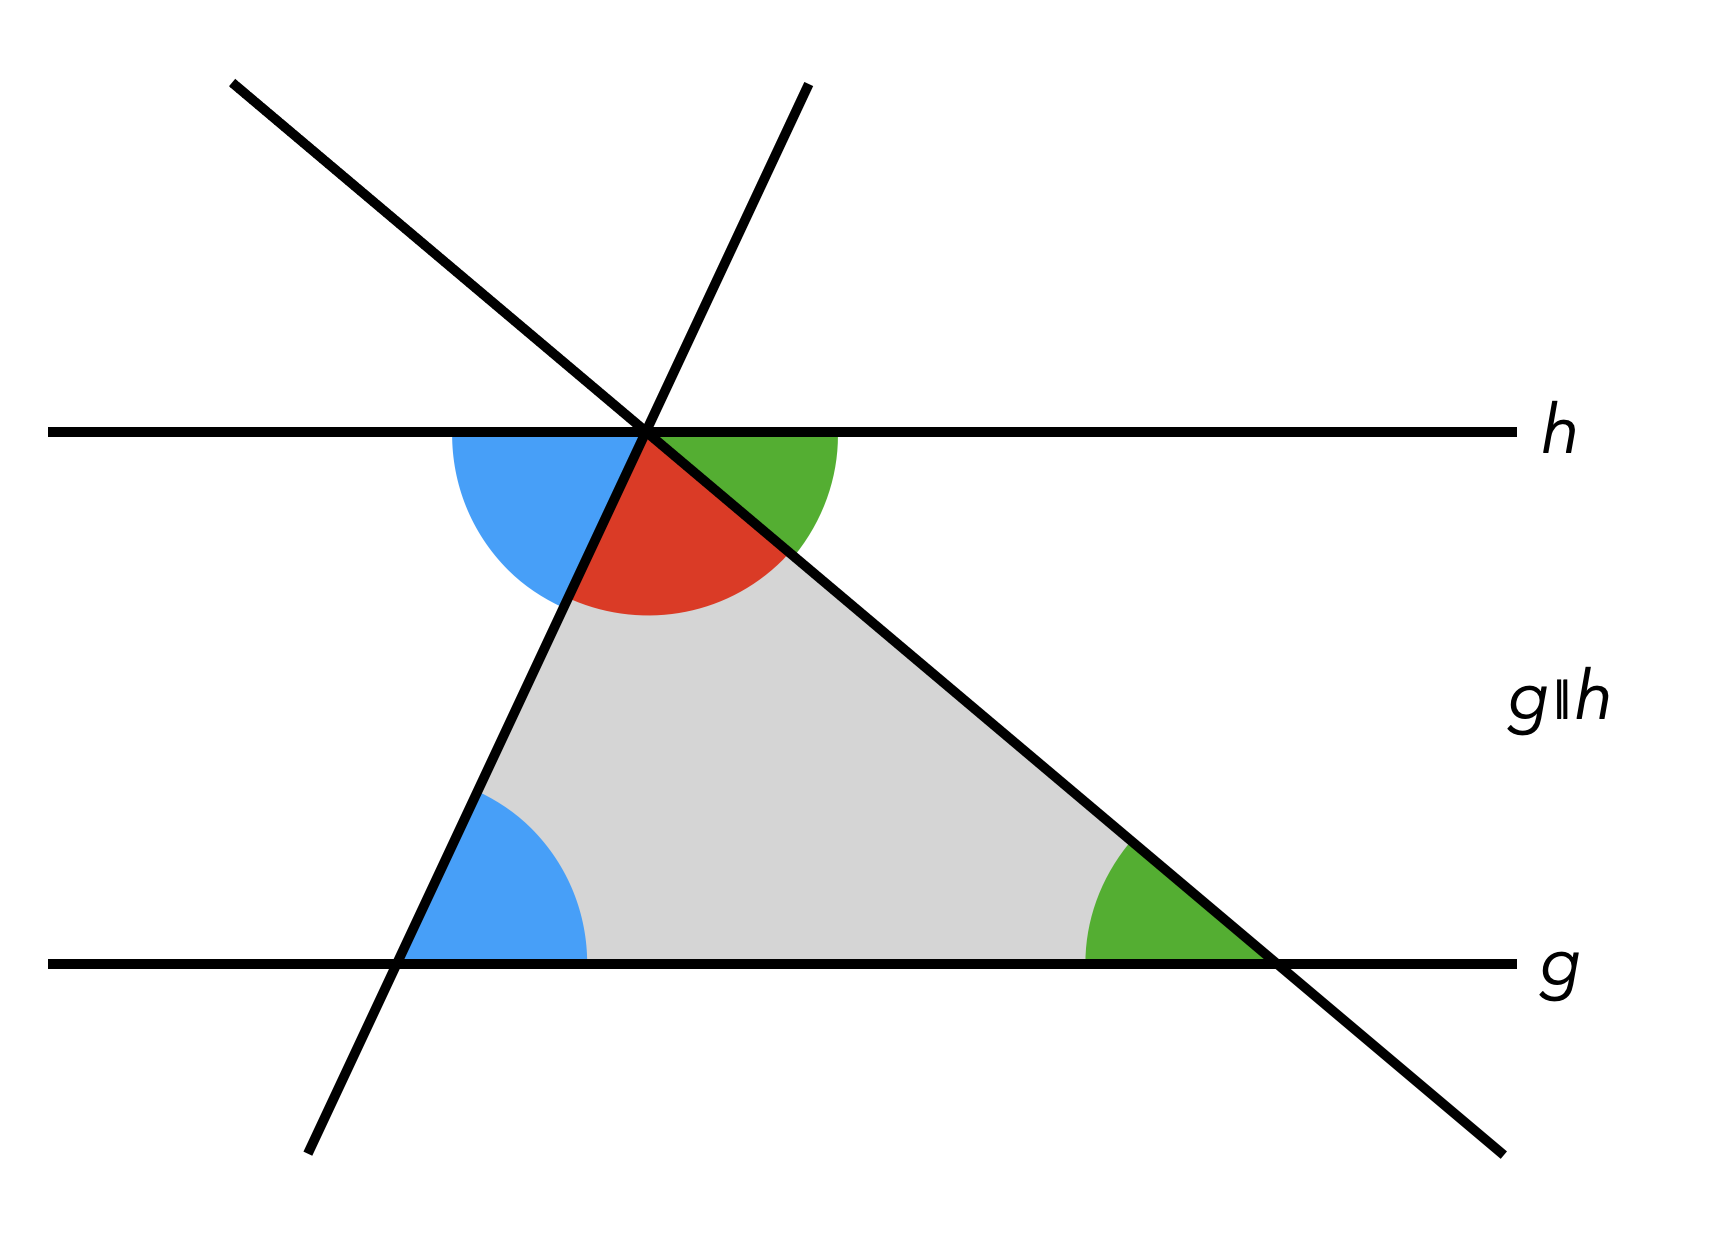
\includegraphics[width=0.75\linewidth]{pictures/C-InnenwinkelBeweisfigur} 

}

\caption{Beweisfigur des Innenwinkelsatzes für Dreiecke}\label{fig:InnenwinkelBeweisfigure}
\end{figure}

\hypertarget{suxe4tze-am-kreis}{%
\subsection{Sätze am Kreis}\label{suxe4tze-am-kreis}}

\hypertarget{zentri-peripheriewinkelsatz}{%
\subsubsection{Zentri-Peripheriewinkelsatz}\label{zentri-peripheriewinkelsatz}}

Der Zentri-Peripheriewinkelsatz besagt, dass der Zentriwinkel über der Sehne eines Kreises stets doppelt so groß ist wie ein Peripheriewinkel auf derselben Seite derselben Sehne (siehe Abbildung \ref{fig:Zentri}).

\begin{figure}

{\centering \includegraphics[width=0.75\linewidth]{pictures/C-Zentri} 

}

\caption{Zentriwinkel (rot) und Peripheriewinkel (blau) auf derselben Seite über derselben Kreissehne}\label{fig:Zentri}
\end{figure}

Um diesen Satz zu beweisen, bedarf es vielfältiger Heurismen, wie das Zeichnen geeigneter Hilfslinien (Radius), die Bezugnahme auf bekannte Sätze (Basiswinkelsatz im gleichschenkligen Dreieck, Innenwinkelsatz im Dreieck) und das Erkennen der Gleichheit von Termen.

\begin{figure}

{\centering \includegraphics[width=0.75\linewidth]{pictures/C-ZentriBeweis} 

}

\caption{Beweisfigur des Zentri-Peripherwiewinkelsatzes}\label{fig:ZentriBeweis}
\end{figure}

Mit den Farben der Winkel aus Abbildung \ref{fig:ZentriBeweis} gilt dann in den jeweiligen Dreiecken:

\[
\begin{aligned}
2\cdot \mathrm{\color{green}{grün}} + 2\cdot \mathrm{\color{orange}{orange}} + 2\cdot \mathrm{\color{purple}{lila}}  &= 180°\\
 \mathrm{\color{red}{rot}} + 2\cdot \mathrm{\color{purple}{lila}} &= 180°
\end{aligned}
\]

Daraus folgt aus dem Vergleich der beiden Zeilen direkt die Aussage des Satzes:

\[\begin{aligned}
\mathrm{\color{red}{rot}} &= 2\cdot \mathrm{\color{green}{grün}} + 2\cdot \mathrm{\color{orange}{orange}} \\
\mathrm{\color{red}{rot}} &= 2\cdot (\mathrm{\color{green}{grün}} +  \mathrm{\color{orange}{orange}}) \\
\mathrm{\color{red}{rot}} &= 2\cdot \mathrm{\color{blue}{blau}}
\end{aligned}
\]
Da der Satz selbst für den weiteren Schulunterricht keine so hohe Bedeutung hat, müssen Sie als Lehrkraft besonders abwägen, ob Sie diesen Beweis besprechen wollen -- auch abhängig von Ihrer Lerngruppe. Im Sinne der Schulung von Heurismen in der Geometrie hat er aber durchaus Potenzial.

\hypertarget{peripheriewinkelsatz}{%
\subsubsection{Peripheriewinkelsatz}\label{peripheriewinkelsatz}}

Der Peripheriewinkelsatz besagt, dass alle Peripheriewinkel auf derselben Seite über derselben Sehne eines Kreises gleich groß sind. Eine Erkundung dieses Satzes ist -- wie beim Innenwinkelsatz für Dreiecke -- bspw. mit Dynamischer Geometriesoftware möglich, indem bei Bewegung des Punktes auf dem Kreis der Peripherwiewinkel permanent gemessen wird.

Formal folgt der Satz direkt aus dem Zentri-Peripherwiewinkelsatz, da der Zentriwinkel bei fester Sehne gleich groß bleibt.

\hypertarget{satz-des-thales}{%
\subsubsection{Satz des Thales}\label{satz-des-thales}}

Eine weitere direkte Folgerung aus dem Zentri-Peripherwiewinkelsatz ist der Satz des Thales, also dass Peripheriewinkel über dem Durchmesser eines Kreises stets \(90°\) betragen. Dies liegt daran, dass der Zentriwinkel in diesem Fall \(180°\) beträgt (siehe Abbildung \ref{fig:Thales}).

\begin{figure}

{\centering \includegraphics[width=0.75\linewidth]{pictures/C-Thales} 

}

\caption{Peripheriewinkel über dem Durchmesser eines Kreises}\label{fig:Thales}
\end{figure}

Der Zusammenhang zwischen Satz des Thales und Zentri-Peripherwiewinkelsatz sollte v.~a. dann hergestellt werden, wenn der Zentri-Peripherwiewinkelsatz intensiv behandelt worden ist. Alternativ lässt sich der Satz des Thales auch direkt beweisen -- und das ist als Spezielfall sogar einfacher als der Beweis des Zentri-Peripherwiewinkelsatzes. Abbildung \ref{fig:ThalesBeweis} zeigt einen Lückentext-Beweis, wie er von Schülerinnen und Schülern durchgeführt werden könnte.



\begin{figure}

{\centering \includegraphics[width=0.75\linewidth]{pictures/C-ThalesBeweis} 

}

\caption{Lückentext-Beweis des Satz des Thales (\protect\hyperlink{ref-Wennekers2016}{Wennekers, 2016, S. 173})}\label{fig:ThalesBeweis}
\end{figure}

\hypertarget{leitidee-funktionaler-zusammenhang}{%
\chapter{Leitidee Funktionaler Zusammenhang}\label{leitidee-funktionaler-zusammenhang}}

\begin{quote}
\textbf{Bedeutsame Lerngegenstände}

\begin{itemize}
\tightlist
\item
  Zuordnungsbegriff
\item
  Proportionalität
\item
  Gleichungen und Ungleichungen
\item
  Terme und Variablen
\item
  Funktionsbegriff
\item
  verschiedene Funktionsklassen (linear, quadratisch, trigonometrisch, \ldots)
\item
  Parametereinfluss
\item
  Gleichungssysteme
\item
  Folgen und Grenzwerte
\item
  Ableitung
\item
  Integral
\item
  Zufallsgröße
\item
  Wahrscheinlichkeitsverteilung
\end{itemize}

\textbf{Literaturempfehlungen}

\begin{itemize}
\tightlist
\item
  \protect\hyperlink{ref-Greefrath2016}{Greefrath et al.} (\protect\hyperlink{ref-Greefrath2016}{2016}): \emph{Didaktik der Analysis. Aspekte und Grundvorstellungen zentraler Begriffe}
\item
  \protect\hyperlink{ref-Danckwerts2010}{Danckwerts \& Vogel} (\protect\hyperlink{ref-Danckwerts2010}{2010}): \emph{Analysis verständlich unterrichten}\\
\item
  \protect\hyperlink{ref-Tietze:2000a}{Tietze et al.} (\protect\hyperlink{ref-Tietze:2000a}{2000a}): \emph{Mathematikunterricht in der Sekundarstufe II. Band 1: Fachdidaktische Grundfragen, Didaktik der Analysis}
\end{itemize}
\end{quote}

\hypertarget{strukturierung-der-leitidee-funktionaler-zusammenhang}{%
\section{Strukturierung der Leitidee}\label{strukturierung-der-leitidee-funktionaler-zusammenhang}}

In den Bildungsstandards für die Primarstufe lautet diese Leitidee »Muster und Strukturen« (\protect\hyperlink{ref-KMK2005}{Sekretariat der Ständigen Konferenz der Kultusminister der Länder in der Bundesrepublik Deutschland, 2005, S. 10~f.}), im Brandenburgischen Rahmenlehrplan wird sie als »Gleichungen und Funktionen« bezeichnet (\protect\hyperlink{ref-MinisteriumfurBildungJugendundSportdesLandesBrandenburg2015a}{Ministerium für Bildung, Jugend und Sport des Landes Brandenburg, 2015b, S. 9}).

Das \protect\hyperlink{ref-LISUMd}{LISUM} (\protect\hyperlink{ref-LISUMd}{o.~J.-d}) hat für die Primarstufe und Sekundarstufe I ein Konzeptbild herausgegeben (siehe Abbildung \ref{fig:KonzeptFunktionen}), ergänzt durch einen didaktischen Kommentar von \protect\hyperlink{ref-Kortenkampa}{Kortenkamp \& Kuzle} (\protect\hyperlink{ref-Kortenkampa}{o.~J.-b}) und Materialien zur Diagnose und Förderung (\protect\hyperlink{ref-LISUMc}{LISUM, o.~J.-c}).



\begin{figure}

{\centering \includegraphics[width=0.9\linewidth]{pictures/D-KonzeptFunktion} 

}

\caption{Konzeptbild zur Leitidee \emph{Gleichungen und Funktionen} (\protect\hyperlink{ref-LISUMd}{LISUM, o.~J.-d})}\label{fig:KonzeptFunktionen}
\end{figure}

\hypertarget{funktionsaspekte}{%
\section{Funktionsaspekte}\label{funktionsaspekte}}

Dreh- und Angelpunkt der Leitidee Funktionaler Zusammenhang und damit auch des Stoffgebiets Analysis ist der \textbf{Funktionsbegriff}. Gemäß der in Kapitel \ref{grundvorstellungen} eingeführten Bezeichnungen können zu drei Grundvorstellungen des Funktionsbegriff Aspekte formuliert werden, hier wörtlich entnommen aus \protect\hyperlink{ref-Greefrath2016}{Greefrath et al.} (\protect\hyperlink{ref-Greefrath2016}{2016, S. 47~ff.})\footnote{Dabei ist zu beachten, dass dort die Bezeichnung \emph{Aspekt} in einer anderen Bedeutung als hier im Dokument verwendet wird, siehe dazu eine Diskussion bei \protect\hyperlink{ref-Etzold2021}{Etzold} (\protect\hyperlink{ref-Etzold2021}{2021, S. 72~f.}).}:

\begin{itemize}
\item
  Grundvorstellung zum \textbf{Zuordnungsaspekt}: »Eine Funktion ordnet jedem Wert einer Größe genau einen Wert einer zweiten Größe zu. Mit dem Mengenbegriff formuliert bedeutet dies: Eine Funktion ordnet jedem Element einer Definitionsmenge genau ein Element einer Zielmenge zu.«

  Typische Repräsentationen dieser Vorstellung sind Wertetabellen oder Pfeildiagramme. Über die (nicht-)Eindeutigkeit abgehender und ankommender Pfeile in der Definitions- und Zielmenge kann bspw. operativ an Beispielen diskutiert werden, ob eine Funktion vorliegt oder nicht. Die einführende Definition des formalen Funktionsbegriffs (meist in Klassenstufe 8) erfolgt in der Regel über den Zuordnungsaspekt -- was die Gefahr einer einseitigen Betrachtung des Begriffs mit sich bringt. Sie müssen sich als Lehrkraft also zunächst einmal der Aspektvielfalt bewusst sein und diese dann auch bei Ihrer Unterrichtsgestaltung beachten.
\item
  Grundvorstellung zum \textbf{Kovariationsaspekt/Änderungsaspekt}: »Mit Funktionen wird erfasst, wie sich Änderungen einer Größe auf eine zweite Größe auswirken bzw. wie die zweite Größe durch die erste beeinflusst wird.«

  Ohne den Kovariationsaspekt ist kein inhaltliches Verständnis von Differenzialrechnung möglich, da der Ableitungsbegriff ja gerade die lokale Änderung einer Funktion beschreibt. Aber auch in der Sekundarstufe I spielt dieser Aspekt schon eine bedeutsame Rolle, bspw. bei der Betrachtung proportionaler Zuordnungen als \emph{gleichmäßige Zunahme} oder wenn unterschiedlich steile lineare Funktionen und das entsprechende Anstiegsdreick behandelt werden.
\item
  Grundvorstellung zum \textbf{Objektaspekt}: »Eine Funktion ist ein einziges Objekt, das einen Zusammenhang als Ganzes beschreibt.«

  Insbesondere bei der Betrachtung von Funktionsgraphen wird ein solcher Gesamtblick geschult und die Funktion als Objekt aufgefasst. Der Objektaspekt ist u.~a. auch bei der Betrachtung des Parametereinflusses von Relevanz, da dort die Funktion \emph{als Ganzes} manipuliert wird. Algebraisch spielt der Aspekt eine Rolle, wenn Funktionsterme addiert werden oder Funktionen bspw. als Elemente eines Vektorraumes aufgefasst werden.
\end{itemize}

\hypertarget{analysis-in-der-sek.-ii}{%
\section{Analysis in der Sek. II}\label{analysis-in-der-sek.-ii}}

\hypertarget{konflikt-zur-fachmathematik}{%
\subsection{Konflikt zur Fachmathematik}\label{konflikt-zur-fachmathematik}}

Der Analysisunterricht in der Schule unterscheidet sich wesentlich von dem in der Hochschule, womit aus fachlicher wie fachdidaktischer Sicht einige Herausforderungen einhergehen. Neben der grundsätzlichen nicht streng deduktiven Herangehensweise werden i.~d.~R. zentrale Begriffe der Analysis im Schulunterricht kaum oder nur propädeutisch-anschaulich behandelt. Die betrifft zunächst einmal den \textbf{Folgen-, Grenzwert- und Stetigkeitsbegriff} (\protect\hyperlink{ref-Danckwerts2010}{Danckwerts \& Vogel, 2010, S. 17~ff.}; \protect\hyperlink{ref-Greefrath2016}{Greefrath et al., 2016, S. 23~ff.}; \protect\hyperlink{ref-Tietze:2000a}{Tietze et al., 2000a, S. 252~ff.}). Der Ableitungsbegriff bedarf bspw. des Grenzwertes des Differenzenquotienten. Ein solcher Grenzwert einer Funktion \(f\) an einer Stelle \(a\) existiert, wenn für alle Folgen \((x_n)_{n\in\mathbb{N}}\) mit \(x_n\rightarrow a\) auch die Folge der Funktionswerte konvergiert, also \(f(x_n)\rightarrow f(a)\). Für den Konvergenzbegriff einer Folge ist nun zum anderen die \textbf{Vollständigkeit der reellen Zahlen} von enormer Bedeutung, was ebenfalls in der Schule nicht in einer derartigen Strenge behandelt wird (siehe z.~B. \protect\hyperlink{ref-Danckwerts2010}{Danckwerts \& Vogel, 2010, S. 27~ff.}). Mathematisch relevant ist für die Konvergenz einer Folge \((x_n)_{n\in\mathbb{N}}\) gegen \(a\) eben nicht nur, dass die Folgenglieder dem \(a\) beliebig nahe kommen, sondern dass \(a\) im betrachteten Zahlbereich tatsächlich existiert. Ein klassisches Beispiel hierfür ist das Heronverfahren zum Wurzelbestimmen. So liefert die rekursive Folge\footnote{Für eine geometrische Interpretation dieser Formel siehe auch \protect\hyperlink{ref-dewiki:216870314}{Wikipedia} (\protect\hyperlink{ref-dewiki:216870314}{2021a}, Abschnitt 2). Hat man diese Interpretation im Hinterkopf, muss man sich nicht einmal die Formel merken.} \(x_{n+1} = \frac{1}{2}\left(x_n + \frac{5}{x_n}\right)\) mit bspw. \(x_0 = 1\) ausschließlich Folgenglieder aus \(\mathbb{Q}\), die sich auch beliebig nahe kommen (eine sogenannte \emph{Cauchy-Folge}), der Grenzwert selbst ist aber \(\sqrt{5}\), was nicht in \(\mathbb{Q}\), sondern nur in \(\mathbb{R}\) liegt.

Ohne derartige zentrale (im fachmathematischen Sinne sauber ausgeprägte) Begriffe Analysisunterricht zu betreiben, bedarf also einer starken Orientierung an den hinter den Begriffen liegenden Grundvorstellungen, damit dennoch ein inhaltlich-anschauliches Verständnis aufgebaut werden kann und der Unterricht nicht zu einem kalkülhaften Vorgehen verkommt. Spezifische Anregungen für einzelne Lerngegenstände bieten die bereits zitierten Quellen.

\hypertarget{beispiel-ableitungsbegriff}{%
\subsection{Beispiel Ableitungsbegriff}\label{beispiel-ableitungsbegriff}}

Für den Ableitungsbegriff (einer Funktion an einer Stelle) haben sich sowohl historisch als auch in der fachdidaktischen Literatur zwei wesentliche Vorstellungen herausgebildet (\protect\hyperlink{ref-Danckwerts2010}{Danckwerts \& Vogel, 2010, S. 45~ff.}; \protect\hyperlink{ref-Greefrath2016}{Greefrath et al., 2016, S. 147~ff.}):

\begin{itemize}
\item
  Grundvorstellung zum Aspekt der \textbf{lokalen Änderungsrate}: Die Ableitung einer Funktion an einer Stelle beschreibt, wie stark sich die Funktionswerte in der Umgebung dieser Stelle verändern. Wird sich dieser Änderungsrate graphisch genähert, erfolgt dies i.~d.~R. durch den Übergang des Anstiegs einer Sekante zu dem einer Tangente\footnote{Zur Diskussion der Vorstellung, was eine Tangente ist, siehe auch \protect\hyperlink{ref-Greefrath2016}{Greefrath et al.} (\protect\hyperlink{ref-Greefrath2016}{2016, S. 149})}, womit die Ableitung über den \textbf{Grenzwert des Differenzenquotienten} \(\lim\limits_{h\rightarrow 0}\cfrac{f(x_0+h)-f(x_0)}{h}\) quantifiziert werden kann und dem \textbf{Anstieg der Tangente} entspricht.

  Diese Sichtweise ermöglicht, den Ableitungbegriff konstruktiv über den Sekanten-Tangenten-Übergang einzuführen und unmittelbar numerisch zu beschreiben. Auch bedienen sich vielfältige Anwendungen (z.~B. Momentan- vs.~Durchschnittsgeschwindigkeit) dieser Vorstellung.
\item
  Grundvorstellung zum Aspekt der \textbf{lokalen Linearität}: Diese Vorstellung betont noch stärker die Differenzierbarkeit als Eigenschaft einer Funktion, nämlich die Möglichkeit, sie lokal durch eine lineare Funktion annähern zu können. Eine typische Repräsentation ist das Heranzoomen an die Funktion, sodass dabei die lokale Linearität besonders deutlich wird. Mathematisch greifbar wird diese Vorstellung darüber, dass sich die Funktion über \(f(x) = f(x_0) + m\cdot r(h)\) beschreiben lässt, wobei der \emph{Fehler} \(r(h)\) so schnell gegen \(0\) geht, dass sogar \(\lim\limits_{h\rightarrow 0}\cfrac{r(h)}{h}=0\) gilt. \(m\) selbst ist dann die Ableitung und der Anstieg der \emph{besten linearen Näherung} -- was natürlich wieder die Tangente an entsprechender Stelle ist.

  Dieses Vorgehen besticht v.~a. durch seine mathematische Verallgemeinerbarkeit für die höherdimensionale Analysis. Auch entspricht es dem Bedürfnis, Prozesse linear zu approximieren (vgl. Abschnitt \ref{beispiel-linearitaet}).
\end{itemize}

\hypertarget{leitidee-daten-und-zufall}{%
\chapter{Leitidee Daten und Zufall}\label{leitidee-daten-und-zufall}}

\begin{quote}
\textbf{Bedeutsame Lerngegenstände}

\begin{itemize}
\tightlist
\item
  Zufallsversuch
\item
  Wahrscheinlichkeit
\item
  Kombinatorik
\item
  Lage- und Streumaße
\item
  Bedingte Wahrscheinlichkeit
\item
  Binomialverteilung
\item
  Normalverteilung
\item
  Hypothesentest
\end{itemize}

\textbf{Literaturempfehlungen}

\begin{itemize}
\tightlist
\item
  \protect\hyperlink{ref-Kruger2015}{Krüger et al.} (\protect\hyperlink{ref-Kruger2015}{2015}): \emph{Didaktik der Stochastik in der Sekundarstufe I}
\item
  \protect\hyperlink{ref-Tietze:2002}{Tietze et al.} (\protect\hyperlink{ref-Tietze:2002}{2002}): \emph{Mathematikunterricht in der Sekundarstufe II. Band 3: Didaktik der Stochastik}
\end{itemize}
\end{quote}

\hypertarget{strukturierung-der-leitidee-daten-und-zufall}{%
\section{Strukturierung der Leitidee}\label{strukturierung-der-leitidee-daten-und-zufall}}

Das \protect\hyperlink{ref-LISUMa}{LISUM} (\protect\hyperlink{ref-LISUMa}{o.~J.-b}) hat für die Primarstufe und Sekundarstufe I ein Konzeptbild herausgegeben (siehe Abbildung \ref{fig:KonzeptDatenZufall}), ergänzt durch einen didaktischen Kommentar von \protect\hyperlink{ref-Kortenkamp}{Kortenkamp \& Kuzle} (\protect\hyperlink{ref-Kortenkamp}{o.~J.-a}) und Materialien zur Diagnose und Förderung (\protect\hyperlink{ref-LISUM}{LISUM, o.~J.-a}).



\begin{figure}

{\centering \includegraphics[width=0.9\linewidth]{pictures/E-KonzeptDatenZufall} 

}

\caption{Konzeptbild zur Leitidee \emph{Daten und Zufall} (\protect\hyperlink{ref-LISUMa}{LISUM, o.~J.-b})}\label{fig:KonzeptDatenZufall}
\end{figure}

In Konzeptbild wird sichtbar, dass der Wahrscheinlichkeitsbegriff die verschiedenen Ideen miteinander in Bezug bringt, was die Bedeutsamkeit von \textbf{stochastischen Vorgängen} für die Leitidee hervorhebt.

\hypertarget{stochastische-vorguxe4nge}{%
\section{Stochastische Vorgänge}\label{stochastische-vorguxe4nge}}

\protect\hyperlink{ref-Kruger2015}{Krüger et al.} (\protect\hyperlink{ref-Kruger2015}{2015, S. 219~f.}) argumentiert, dass der häufig verbreitete Begriff des \textbf{Zufallsexperiments} aus fachlicher wie didaktischer Sicht ungeeignet für den Unterricht erscheint. Er begründet dies u.~a. mit der Nichtnotwendigkeit des Begriffs in der Fachmathematik und damit, dass es sich nicht um ein \emph{Experiment} im naturwissenschaftlichen Sinne der Hypothesenüberprüfung unter kontrollierten Bedingungen handele -- die oftmals formulierte Regel der »beliebige{[}n{]} Wiederholbarkeit unter gleichen Bedingungen« sei letztlich schon ein Modell mit der Annahme der stochastischen Unabhängigkeit (\protect\hyperlink{ref-Kruger2015}{Krüger et al., 2015, S. 219}). Spiele, in denen der Zufall eine Rolle spielt, sind für den Mathematikunterricht höchst relevant -- sollten aber nicht als Experimente aufgefasst werden. Stattdessen werden für die Grundschule der Begriff \textbf{Vorgang mit mehreren möglichen Ergebnissen} und für die weiterführenden Schulen der Begriff \textbf{stochastischer Vorgang} vorgeschlagen (\protect\hyperlink{ref-Kruger2015}{Krüger et al., 2015, S. 220})

Für die tatsächliche Unterrichtsausführung ist dies insofern problematisch, da der Begriff \emph{Zufallsexperiment} i.~d.~R. Bestandtteil der Lehrpläne ist (siehe z.~B. \protect\hyperlink{ref-MinisteriumfurBildungJugendundSportdesLandesBrandenburg2015a}{Ministerium für Bildung, Jugend und Sport des Landes Brandenburg, 2015b, S. 59, 61}) und damit unterrichtet werden muss. Sie als Lehrkraft sollten also stets die an der Verwendung des Begriffs vorgebrachte Kritik im Hinterkopf haben und dies sensibel bei Ihrer Unterrichtsgestaltung beachten. Dies kann etwa bedeuten, dass Sie dennoch eine \emph{übliche} Definition des Begriffs Zufallsexperiment nutzen (siehe Abbildung \ref{fig:DefinitionZufallsexperiment}), aber im Unterricht die Unterschiede zu \emph{echten} Experimenten thematisieren und über geeignete Beispiele und Gegenbeispiele den Begriff ausschärfen.



\begin{figure}

{\centering \includegraphics[width=0.75\linewidth]{pictures/E-DefinitionZufallsexperiment} 

}

\caption{Schulbuchdefinition des Begriff \emph{Zufallsexperiment} (\protect\hyperlink{ref-Adam2016}{Adam \& Kleine, 2016, S. 18})}\label{fig:DefinitionZufallsexperiment}
\end{figure}

Grundsätzlich ist es Aufgabe der Stochastik, reale Prozesse zu modellieren, um diese mit mathematischen Mitteln greifbar (und bearbeitbar) zu machen. Dazu ist es normalerweise notwendig, die reale Situation zu vereinfachen und in ein \emph{Realmodell} überzuführen (siehe Abbildung \ref{fig:Modelle}. Der Begriff \emph{stochastischer Vorgang} ist dann »auf der Ebene der Realmodelle angesiedelt«, mit der Verwendung des Begriffs \emph{Zufallsexperiment} dagegen »verwischt man die Grenzen zwischen Realität und Modellebene« (\protect\hyperlink{ref-Kruger2015}{Krüger et al., 2015, S. 219~f.}).



\begin{figure}

{\centering \includegraphics[width=0.75\linewidth]{pictures/E-Modelle} 

}

\caption{Modellierungsstruktur in der Stochastik (\protect\hyperlink{ref-Kruger2015}{Krüger et al., 2015, S. 13})}\label{fig:Modelle}
\end{figure}

Aufbauend auf diese Struktur (die »nicht als expliziter Gegenstand des Stochastikunterrichts aufzufassen« ist, \protect\hyperlink{ref-Kruger2015}{Krüger et al., 2015, S. 13}) können Sie Ihre Diskussionen im Unterricht leiten und Schwierigkeiten der Schülerinnen und Schüler besser einordnen, z.~B.:

\begin{itemize}
\item
  Wenn ein Würfel geworfen wird (reale Situation) und man die Wahrscheinlichkeit für eine Augenzahl angibt (theoretisches Modell), geht man davon aus, dass der Würfel aus sechs identischen Seiten besteht und in sich homogen ist (Realmodell). Mögliche Fragen, die auf eine solche Denkweise hinarbeiten, könnten sein: \emph{Welche Annahmen triffst du? Welche Eigenschaften muss der Würfel haben, damit du so rechnen darfst?}
\item
  Wenn erstmals \emph{Zufallsgeräte} (übrigens auch ein Begriff auf der Ebene der Realmodelle) genutzt werden, muss eine Untergeneralisierung vermieden werden, es sollten also frühzeitig auch nicht-Laplace-Geräte eingesetzt werden, wie Reißzwecken, Quader, sogenannte Riemer-Würfel (\protect\hyperlink{ref-Riemer1988}{Riemer, 1988}) oder auch \emph{Würfel-Schweine} (\protect\hyperlink{ref-dewiki:214496187}{Wikipedia, o.~J.}).
\item
  Wenn eine Schülerin oder ein Schüler nicht in der Lage ist, für das Ziehen einer Herz-Karte aus einem Skatblatt die Wahrscheinlichkeit anzugeben, sollten Sie als Lehrkraft herausfinden, auf welcher Ebene Schwierigkeiten bestehen. Wird die reale Situation nicht verstanden (weil z.~B. die Spielkartenfarben oder der Begriff \emph{Skatblatt} unbekannt sind)? Bestehen Schwierigkeiten im Aufstellen eines Realmodells (dass also das Ziehen jeder Karte mit derselben Wahrscheinlichkeit verbunden ist und dafür die Anzahl der relevanten Karten bestimmt werden muss)? Oder sind Defizite in der Theorie verortet (weil etwa nicht die Laplace-Formel für die Berechnung der Wahrscheinlichkeit angewandt werden kann oder gar Schwierigkeiten bei der Division bestehen)?
\end{itemize}

\hypertarget{lagemauxdfe}{%
\section{Lagemaße}\label{lagemauxdfe}}

Während der Vorlesungsveranstaltung wurde ein virtuelles Arbeitsmittel\footnote{zum Begriff des Arbeitsmittels siehe Kapitel zu \protect\hyperlink{lernumgebungen}{Lernumgebungen}} mit Cinderalla und CindyScript (vgl. \protect\hyperlink{ref-Richter-Gebert2012}{Richter-Gebert \& Kortenkamp, 2012}) zur Erkundung von \textbf{arithmetischem Mittel} und \textbf{Median} erstellt. Abbildung \ref{fig:ScreenshotLagemass} zeigt einen Screenshot des \href{files/Stoffdidaktik-WiSe2122-AnhangE-Lagemasse.html}{virtuellen Arbeitsmittels}, das auch als \href{files/Stoffdidaktik-WiSe2122-AnhangE-Lagemasse.cdy}{Cinderella-Datei} zur Verfügung steht.

\begin{figure}

{\centering \includegraphics[width=0.75\linewidth]{pictures/E-ScreenshotLagemass} 

}

\caption{Screenshot des virtuellen Arbeitsmittels zu Lagemaßen}\label{fig:ScreenshotLagemass}
\end{figure}

Anregungen für Aufgabenstellungen, die zu einer vertiefenden Beschäftigung mit den beiden Lagemaßen unter Zuhilfenahme des Arbeitsmittes führen können, sind zum Beispiel:

\begin{itemize}
\tightlist
\item
  \emph{Verändere die Punkte so, dass Median und arithmetisches Mittel gleich sind.}
\item
  \emph{Kannst du Punkte verschieben, so dass Median oder arithmetisches Mittel unverändert bleiben? Bei welchen Punkten geht das (nicht) und warum (nicht)?}
\item
  \emph{Wie verändert sich das beobachtete Verhalten von arithmetischem Mittel und Median bei ungerader Anzahl an Punkten?}
\item
  \emph{Zeige mit dem Arbeitsmittel, dass der Median stabil gegenüber Ausreißern ist, das arithmetische Mittel jedoch nicht.}
\end{itemize}

\hypertarget{seminar-und-hausarbeit}{%
\chapter{Seminar und Hausarbeit}\label{seminar-und-hausarbeit}}

\hypertarget{hausarbeit}{%
\section{Hausarbeit}\label{hausarbeit}}

\hypertarget{aufgabenstellung}{%
\subsection{Aufgabenstellung}\label{aufgabenstellung}}

Erstellen Sie eine \textbf{ausführliche stoffdidaktische} Analyse zu einem bestimmten Lerngegenstand. Das heißt konkret:

\begin{itemize}
\tightlist
\item
  Beantworten Sie inhaltlich die Fragen der \textbf{formalen, semantischen und konkreten Ebene} des Vier-Ebenen-Ansatzes. Es ist jedoch nicht notwendig, die Fragen einzeln »abzuarbeiten« -- vielmehr geht es darum, dass Sie in Ihrer Darstellung deutlich machen, all die verschiedenen Punkte beachtet zu haben. Sie können natürlich auch Schwerpunkte legen und müssen nicht alle Fragen in gleicher Qualität bzw. Quantität beantworten. Wenn Sie geeignete Quellen finden, können Sie auch auf die empirische Ebene eingehen.
\item
  Nutzen Sie für Ihre Analyse \textbf{geeignete fachmathematische und fachdidaktische Literatur sowie ggf. auch Schulbücher}. Sie müssen die einzelnen Ebenen nicht zwingend getrennt betrachten, können dies aber, wenn es sich anbietet (z.~B. ist es häufig sinnvoll, die konkrete Ebene im Anschluss an die formale und semantische zu betrachten).
\item
  Als Ergebnis der Analyse soll ein möglicher \textbf{Lernpfad} stehen, anhand dessen der Lerngegenstand im Unterricht behandelt werden kann. Es ist also insbesondere auch möglich, einen bereits existierenden Lernpfad (z.~B. aus einem Schulbuch oder einer fachdidaktischen Literatur) zu nutzen und diesen mittels der stoffdidaktischen Analyse zu begründen (bzw. ggf. Änderungen vorzuschlagen).
\item
  Gehen Sie im Rahmen Ihrer Entwicklung des Lernpfades auf \textbf{einen der folgenden Punkte} besonders ein (wenden Sie also die in der Vorlesung vermittelte Theorie auf Ihren Lerngegenstand an):

  \begin{itemize}
  \tightlist
  \item
    Möglichkeiten der Begriffseinführung und Nutzung von Beispielen und Gegenbeispielen
  \item
    Nutzung bestimmter Arbeitsmittel zur Unterstützung des vermittelten Lerninhalts
  \item
    Gestaltung konkreter Aufgabenstellungen für die Behandlung des Themas
  \end{itemize}
\end{itemize}

\hypertarget{bewertungskriterien}{%
\subsection{Bewertungskriterien}\label{bewertungskriterien}}

\textbf{Ausreichende Leistung (4,0):} Die Analyse der formalen, semantischen und konkreten Ebene ist erkennbar und fachlich im Wesentlichen korrekt. Es wird geeignete Literatur verwendet. Einer der Schwerpunkte (Begriffsbildung, Arbeitsmittel oder Aufgaben) wird aufgegriffen.

\textbf{Befriedigende Leistung (3,0):} Zusätzlich: Die Analyse auf der formalen, semantischen und konkreten Ebene wird vollständig durchgeführt. Die Literatur wird korrekt und einheitlich zitiert. Der Schwerpunkt wird ausführlich am gewählten Lerngegenstand dargestellt.

\textbf{Gute Leistung (2,0):} Zusätzlich: Die Analyse wird sprachlich überzeugend dargestellt und es wird sinnvoll logisch argumentiert. Inhaltlich werden geeignete Querbezüge hergestellt, z.~B. zu anderen Lerngegenständen, fachmathematischen Inhalten bzw. zu weiteren (fach-)didaktischen, pädagogischen oder lernpsychologischen Theorien, \ldots{}

\textbf{Sehr gute Leistung (1,0):} Die Arbeit übertrifft bei Weitem die vorherigen Anforderungen, z.~B. wird auch auf die empirische Ebene eingegangen oder es wird auf mehrere Schwerpunkte eingegangen oder es wird anderweitig eine besonders kreative Leistung sichtbar.

Entsprechende Abstufungen (+/-- 0,3) sind möglich.

\hypertarget{formale-hinweise}{%
\subsection{Formale Hinweise}\label{formale-hinweise}}

\begin{itemize}
\tightlist
\item
  Die Hausarbeit soll 6 bis 8 Textseiten beinhalten (ohne Deckblatt, Inhaltsverzeichnis, Literaturverzeichnis, Anhang, \ldots), wobei natürlich geeignete Abbildungen in den 6 bis 8 Seiten enthalten sein können.
\item
  Es ist angedacht, die Hausarbeit im Nachgang den anderen Studierenden zur Verfügung zu stellen -- gern auch im Anschluss an eine freiwillige Überarbeitung nach erhaltenen Rückmeldungen. Für die weitere Verwendung Ihrer Arbeit beachten Sie bitte:

  \begin{itemize}
  \tightlist
  \item
    Nummerieren Sie Ihre Seiten durch, so dass die auf dem Blatt stehende Seitenzahl auch der Seitenzahl der pdf-Datei entspricht.
  \item
    Verzichten Sie auf Leerseiten.
  \item
    Auf dem Deckblatt der Arbeit sollte Ihr Name, das Thema und Abgabedatum stehen, nicht jedoch Ihre Matrikelnummer, Adresse oder andere persönliche Daten (siehe Beispiel in Abbildung \ref{fig:BeispielDeckblatt}).
  \end{itemize}
\end{itemize}

\begin{figure}

{\centering \includegraphics[width=0.5\linewidth]{pictures/F-abb-BeispielDeckblatt} 

}

\caption{Beispielhaftes Deckblatt für Hausarbeit}\label{fig:BeispielDeckblatt}
\end{figure}

\hypertarget{seminarvortrag}{%
\section{Seminarvortrag}\label{seminarvortrag}}

Stellen Sie in einer \textbf{ansprechenden Seminarsitzung} einen \textbf{Lernpfad zu Ihrem gewählten Lerngegenstand} vor.

\begin{itemize}
\tightlist
\item
  Planen Sie etwa \textbf{30 bis 45 Minuten} ein -- je nachdem, wie viele interaktive Elemente Sie mit Ihren Kommiliton/-innen einsetzen. Im Anschluss sollte auf jeden Fall noch Raum für Rückfragen bestehen. Pro Thema stehen insgesamt 60 Minuten zur Verfügung.
\item
  Ihre Seminarsitzung soll \textbf{Lust darauf machen}, das jeweilige Thema zu unterrichten. Dabei muss sichtbar werden, dass Sie den \textbf{Lernpfad fachlich und fachdidaktisch professionell begründen} können, also auf formaler, semantischer und konkreter Ebene einer stoffdidaktischen Analyse einordnen können.
\item
  Es ist nicht zwingend nötig, eine vollständige und strukturierte stoffdidaktische Analyse zu präsentieren (das machen Sie ja in der Hausarbeit), aber Sie sollten Klarheit über die einzelnen Bestandteile haben, um auch \textbf{souverän auf Rückfragen reagieren} zu können.
\item
  Bezüglich der Vorlesungsinhalte sollten in der Seminarsitzung \textbf{zwei Schwerpunkte} aus der folgenden Auswahl im Zusammenhang mit Ihrem Lerngegenstand sichtbar werden:

  \begin{itemize}
  \tightlist
  \item
    Grundvorstellungen
  \item
    Wege zur Begriffsbildung
  \item
    Tätigkeitstheoretische Hintergründe von Lehr-Lern-Prozessen
  \item
    Präsentation und Analyse eines (analogen oder digitalen) Arbeitsmittels
  \item
    Diskussion konkreter Aufgabenstellungen
  \end{itemize}
\end{itemize}

\hypertarget{vollstuxe4ndiges-literaturverzeichnis}{%
\chapter*{Vollständiges Literaturverzeichnis}\label{vollstuxe4ndiges-literaturverzeichnis}}
\addcontentsline{toc}{chapter}{Vollständiges Literaturverzeichnis}

\hypertarget{refs}{}
\begin{CSLReferences}{1}{0}
\leavevmode\vadjust pre{\hypertarget{ref-Adam2016}{}}%
Adam, V., \& Kleine, M. (2016). \emph{Mathe.delta: {Mathematik} für das {Gymnasium} 8, {Berlin}/{Brandenburg}}. C.C.Buchner.

\leavevmode\vadjust pre{\hypertarget{ref-Barzel2012a}{}}%
Barzel, B., Hußmann, S., Leuders, T., \& Prediger, S. (Hrsg.). (2012a). \emph{Mathewerkstatt. 5, {Handreichungen}} {[}DVD{]}. Cornelsen.

\leavevmode\vadjust pre{\hypertarget{ref-Barzel2012b}{}}%
Barzel, B., Hußmann, S., Leuders, T., \& Prediger, S. (Hrsg.). (2012b). \emph{Mathewerkstatt. 5, {Materialblock}} (Mittlerer Schulabschluss, allgemeine Ausg., 1. Aufl). Cornelsen.

\leavevmode\vadjust pre{\hypertarget{ref-Barzel2012}{}}%
Barzel, B., Hußmann, S., Leuders, T., \& Prediger, S. (Hrsg.). (2012c). \emph{Mathewerkstatt. 5, {Schulbuch}} (Mittlerer Schulabschluss, allgemeine Ausg., 1. Aufl.). Cornelsen.

\leavevmode\vadjust pre{\hypertarget{ref-Barzel2016}{}}%
Barzel, B., Hußmann, S., Leuders, T., \& Prediger, S. (Hrsg.). (2016). \emph{Mathewerkstatt. 9, {Schulbuch}} (Mittlerer Schulabschluss, allgemeine Ausg., 1. Aufl.). Cornelsen.

\leavevmode\vadjust pre{\hypertarget{ref-Bender1978}{}}%
Bender, P. (1978). Umwelterschließung im {Geometrieunterricht} durch operative {Begriffsbildung}. \emph{Der Mathematikunterricht}, \emph{5}(78), 25--87. \url{https://digital.ub.uni-paderborn.de/hsx/download/pdf/42114?originalFilename=true}

\leavevmode\vadjust pre{\hypertarget{ref-Bruckler:2018}{}}%
Brückler, F. M. (2018). \emph{Geschichte der {Mathematik} kompakt: {Das} {Wichtigste} aus {Analysis}, {Wahrscheinlichkeitstheorie}, angewandter {Mathematik}, {Topologie} und {Mengenlehre}}. Springer Spektrum. \url{https://doi.org/10.1007/978-3-662-55574-3}

\leavevmode\vadjust pre{\hypertarget{ref-Bruder}{}}%
Bruder, R. (o.~J.). \emph{Eine akzentuierte {Aufgabenauswahl} und {Vermitteln} heuristischer {Erfahrung} -- {Wege} zu einem anspruchsvollen {Mathematikunterricht} für alle}. Abgerufen 2. Januar 2022, von \url{http://www.math-learning.com/files/extremal.pdf}

\leavevmode\vadjust pre{\hypertarget{ref-Bruder2012}{}}%
Bruder, R. (2012). Vielseitig mit {Aufgaben} arbeiten -- {Mathematische} {Kompetenzen} nachhaltig entwickeln und sichern. In R. Bruder, T. Leuders, \& A. Büchter (Hrsg.), \emph{Mathematikunterricht entwickeln} (S. 18--52). Cornelsen Scriptor.

\leavevmode\vadjust pre{\hypertarget{ref-Bruder2015a}{}}%
Bruder, R., Linneweber-Lammerskitten, H., \& Reibold, J. (2015). Individualisieren und differenzieren. In R. Bruder, L. Hefendehl-Hebeker, B. Schmidt-Thieme, \& H.-G. Weigand (Hrsg.), \emph{Handbuch der {Mathematikdidaktik}} (S. 513--534). Springer Berlin Heidelberg. \url{https://doi.org/10.1007/978-3-642-35119-8_19}

\leavevmode\vadjust pre{\hypertarget{ref-Bruner:1976}{}}%
Bruner, J. S. (1976). Die {Bedeutung} der {Struktur} im {Lernprozeß}. In A. Holtmann (Hrsg.), \emph{Das sozialwissenschaftliche {Curriculum} in der {Schule}: {Neue} {Formen} und {Inhalte}} (S. 77--90). VS Verlag für Sozialwissenschaften. \url{https://doi.org/10.1007/978-3-322-85275-5}

\leavevmode\vadjust pre{\hypertarget{ref-BundesministeriumfurErnahrungundLandwirtschaft2014}{}}%
Bundesministerium für Ernährung und Landwirtschaft. (2014). \emph{Gutachten über {Mindestanforderungen} an die {Haltung} von {Säugetieren}}. \url{https://www.bmel.de/SharedDocs/Downloads/DE/_Tiere/Tierschutz/HaltungSaeugetiere.pdf;jsessionid=6B0914AB410E7E118E6CC87C65735734.live832?__blob=publicationFile\&v=7}

\leavevmode\vadjust pre{\hypertarget{ref-Danckwerts:1988}{}}%
Danckwerts, R. (1988). Linearität als organisierendes Element zentraler Inhalte der Schulmathematik. \emph{Didaktik der Mathematik}, \emph{16}(2), 149--160.

\leavevmode\vadjust pre{\hypertarget{ref-Danckwerts2010}{}}%
Danckwerts, R., \& Vogel, D. (2010). \emph{Analysis verständlich unterrichten} (1. Aufl., 2. Nachdruck). Spektrum Akad. Verl.

\leavevmode\vadjust pre{\hypertarget{ref-Drijvers2010}{}}%
Drijvers, P., Doorman, M., Boon, P., Reed, H., \& Gravemeijer, K. (2010). The teacher and the tool: instrumental orchestrations in the technology-rich mathematics classroom. \emph{Educational Studies in Mathematics}, \emph{75}(2), 213--234. \url{https://doi.org/10.1007/s10649-010-9254-5}

\leavevmode\vadjust pre{\hypertarget{ref-Druke-Noe2018}{}}%
Drüke-Noe, C. (2018). Einfach -- mittel -- schwierig \ldots{} {Wenn} das so einfach wäre: {Aufgaben} unterschiedlichen {Schwierigkeitsgrades} entwickeln. \emph{mathematik lehren}, \emph{209}, 9--12.

\leavevmode\vadjust pre{\hypertarget{ref-DZLM}{}}%
DZLM. (o.~J.). \emph{Anzahlen strukturieren}. Abgerufen 18. Februar 2022, von \url{https://pikas-mi.dzlm.de/node/122}

\leavevmode\vadjust pre{\hypertarget{ref-Etzold:2019}{}}%
Etzold, H. (2019a). \emph{Winkel-{Farm}} (Version 2) {[}App{]}. \url{https://apps.apple.com/de/app/winkel-farm/id1369585218}

\leavevmode\vadjust pre{\hypertarget{ref-Etzold:2019Praxis4}{}}%
Etzold, H. (2019b). \emph{Winkel-{Farm} -- {Leitfaden} für {Lehrerinnen} und {Lehrer}} (Version 2). Zenodo. \url{https://doi.org/10.5281/zenodo.4747700}

\leavevmode\vadjust pre{\hypertarget{ref-Etzold2020a}{}}%
Etzold, H. (2020). \emph{Klipp {Klapp}} {[}App{]}. \url{https://apps.apple.com/de/app/klipp-klapp/id1157365733}

\leavevmode\vadjust pre{\hypertarget{ref-Etzold2021}{}}%
Etzold, H. (2021). \emph{Neue Zugänge zum Winkelbegriff} {[}Dissertation, Universität Potsdam{]}. \url{https://doi.org/10.25932/publishup-50418}

\leavevmode\vadjust pre{\hypertarget{ref-Etzold2018}{}}%
Etzold, H., Kortenkamp, U., \& Ladel, S. (2018). {ACAT}-{Review}-{Guide} -- {Ein} tätigkeitstheoretischer {Blick} auf die {Beurteilung} von {Mathematik}-{Apps}. In S. Ladel, U. Kortenkamp, \& H. Etzold (Hrsg.), \emph{Mathematik mit digitalen {Medien} -- konkret} (S. 91--98). WTM-Verlag. \url{https://doi.org/10.37626/GA9783959870788.0.07}

\leavevmode\vadjust pre{\hypertarget{ref-Etzold2014a}{}}%
Etzold, H., \& Petzschler, I. (2014). \emph{Mathe verstehen durch {Papierfalten}}. Verlag an der Ruhr.

\leavevmode\vadjust pre{\hypertarget{ref-Fockler2018}{}}%
Föckler, F., Leuders, T., \& Holzäpfel, L. (2018). Die selbstdifferenzierende {Aufgabe} als {Form} der {Differenzierung} im {Mathematikunterricht}. In Fachgruppe Didaktik der Mathematik der Universität Paderborn (Hrsg.), \emph{Beiträge zum {Mathematikunterricht} 2018} (S. 541--544). WTM. \url{https://doi.org/10.17877/DE290R-19327}

\leavevmode\vadjust pre{\hypertarget{ref-Franke2016}{}}%
Franke, M., \& Reinhold, S. (2016). \emph{Didaktik der {Geometrie}. {In} der {Grundschule}} (3. Aufl.). Springer Spektrum.

\leavevmode\vadjust pre{\hypertarget{ref-Freudenthal:1973}{}}%
Freudenthal, H. (1973). \emph{Mathematik als pädagogische {Aufgabe}} (Bd. 2). Klett.

\leavevmode\vadjust pre{\hypertarget{ref-Giest2016a}{}}%
Giest, H. (2016). Kulturhistorische {Didaktik} und {Bildungstheorie}. \emph{Tätigkeitstheorie. Journal für tätigkeitstheoretische Forschung in Deutschland}, \emph{14}, 24--48. \url{http://www.ich-sciences.de/media/journal/Ausgabe_14/heft_14.pdf}

\leavevmode\vadjust pre{\hypertarget{ref-Giest2004a}{}}%
Giest, H., \& Lompscher, J. (2004). Tätigkeitstheoretische Überlegungen zu einer neuen {Lernkultur}. \emph{Sitzungsberichte der Leibniz-Sozietät}, \emph{72}, 101--123. \url{https://leibnizsozietaet.de/wp-content/uploads/2012/11/07_giest.pdf}

\leavevmode\vadjust pre{\hypertarget{ref-Giest2006}{}}%
Giest, H., \& Lompscher, J. (2006). \emph{Lerntätigkeit -- {Lernen} aus kultur-historischer {Perspektive}. {Ein} {Beitrag} zur {Entwicklung} einer neuen {Lernkultur} im {Unterricht}}. Lehmanns Media.

\leavevmode\vadjust pre{\hypertarget{ref-Greefrath2016}{}}%
Greefrath, G., Oldenburg, R., Siller, H.-S., Ulm, V., \& Weigand, H.-G. (2016). \emph{Didaktik der {Analysis}. {Aspekte} und {Grundvorstellungen} zentraler {Begriffe}} (F. Padberg \& A. Büchter, Hrsg.; 4. Aufl.). Springer Spektrum. \url{https://doi.org/10.1007/978-3-662-48877-5}

\leavevmode\vadjust pre{\hypertarget{ref-Hattermann2014}{}}%
Hattermann, M., Hofe, R. vom, \& Viehmeister, F. (2014). Rote {Karte}? {Ich} hab' grün! {Ein} {Spiel} zur {Addition} und {Subtraktion} ganzer {Zahlen}. \emph{mathematik lehren}, \emph{183}, 15--19.

\leavevmode\vadjust pre{\hypertarget{ref-Hefendehl-Hebeker:2016}{}}%
Hefendehl-Hebeker, L. (2016). Subject-matter didactics in {German} traditions: {Early} historical developments. \emph{Journal für Mathematik-Didaktik}, \emph{37}(S1), 11--31. \url{https://doi.org/10.1007/s13138-016-0103-7}

\leavevmode\vadjust pre{\hypertarget{ref-Hussmann:2016}{}}%
Hußmann, S., \& Prediger, S. (2016). Specifying and Structuring Mathematical Topics: A Four-Level Approach for Combining Formal, Semantic, Concrete, and Empirical Levels Exemplified for Exponential Growth. \emph{Journal für Mathematik-Didaktik}, \emph{37}(S1), 33--67. \url{https://doi.org/10.1007/s13138-016-0102-8}

\leavevmode\vadjust pre{\hypertarget{ref-Hussmann:2016a}{}}%
Hußmann, S., Rezat, S., \& Sträßer, R. (2016). Subject {Matter} {Didactics} in {Mathematics} {Education}. \emph{Journal für Mathematik-Didaktik}, \emph{37}(S1), 1--9. \url{https://doi.org/10.1007/s13138-016-0105-5}

\leavevmode\vadjust pre{\hypertarget{ref-InstitutfurQualitatsentwicklungimBildungswesen2019}{}}%
Institut für Qualitätsentwicklung im Bildungswesen. (2019). \emph{Gemeinsame {Aufgabenpools} der {Länder}. {Aufgaben} für das {Fach} {Mathematik}. {Grundstock} von {Operatoren}}. \url{https://www.iqb.hu-berlin.de/abitur/abitur/dokumente/mathematik/M_Grundstock_von.pdf}

\leavevmode\vadjust pre{\hypertarget{ref-Jahnke:2010}{}}%
Jahnke, T. (2010). Vom mählichen {Verschwinden} des {Fachs} aus der {Mathematikdidaktik}. \emph{GDM-Mitteilungen 89}, 21--24. \url{https://ojs.didaktik-der-mathematik.de/index.php/mgdm/article/view/559/550}

\leavevmode\vadjust pre{\hypertarget{ref-Kleine2011}{}}%
Kleine, M. (Hrsg.). (2011). \emph{Mathe.{Logo}. 5, {Schülerband}} (Sekundarstufe I, 2. Aufl). Buchner.

\leavevmode\vadjust pre{\hypertarget{ref-Kleine2011a}{}}%
Kleine, M., \& Ludwig, M. (Hrsg.). (2011). \emph{Mathe.{Logo}. 7, {Gymnasium} {Thüringen}, {Schülerband}} (1. Auflage). C.C.Buchner.

\leavevmode\vadjust pre{\hypertarget{ref-Kortenkamp2019}{}}%
Kortenkamp, U., Etzold, H., \& Ladel, S. (2019). \emph{Leitfaden zur {Beurteilung} von {Apps}}. Zenodo. \url{https://doi.org/10.5281/zenodo.5091906}

\leavevmode\vadjust pre{\hypertarget{ref-Kortenkamp}{}}%
Kortenkamp, U., \& Kuzle, A. (o.~J.-a). \emph{Materialien zur {Diagnose} und {Förderung} im {Mathematikunterricht} -- {Leitidee} „{Daten} und {Zufall}``. {Didaktischer} {Kommentar}}. Abgerufen 25. Januar 2022, von \url{https://bildungsserver.berlin-brandenburg.de/fileadmin/bbb/unterricht/faecher/naturwissenschaften/mathematik/Materialien_zur_Diagnose_und_Foerderung_im_Mathematikunterricht/Daten_und_Zufall/059_Daten_und_Zufall_didaktischer_Kommentar_181019.pdf}

\leavevmode\vadjust pre{\hypertarget{ref-Kortenkampa}{}}%
Kortenkamp, U., \& Kuzle, A. (o.~J.-b). \emph{Materialien zur {Diagnose} und {Förderung} im {Mathematikunterricht} -- {Leitidee} „{Gleichungen} und {Funktionen}``. {Didaktischer} {Kommentar}}. Abgerufen 25. Januar 2022, von \url{https://bildungsserver.berlin-brandenburg.de/fileadmin/bbb/rlp-online/Teil_C/Mathematik/Materialien/Materialien_zum_Themenfeld_Gleichungen_und_Funktionen/008_L4_Didaktischer_Text.pdf}

\leavevmode\vadjust pre{\hypertarget{ref-Kortenkampb}{}}%
Kortenkamp, U., \& Kuzle, A. (o.~J.-c). \emph{Materialien zur {Diagnose} und {Förderung} im {Mathematikunterricht} -- {Leitidee} „{Größen} und {Messen}``. {Didaktischer} {Kommentar}}. Abgerufen 18. Februar 2022, von \url{https://bildungsserver.berlin-brandenburg.de/fileadmin/bbb/unterricht/faecher/naturwissenschaften/mathematik/Materialien_zur_Diagnose_und_Foerderung_im_Mathematikunterricht/Groessen_und_Messen/008_Gri_en_und_Messen_didaktischer_Text_181019.pdf}

\leavevmode\vadjust pre{\hypertarget{ref-Krainer:1989}{}}%
Krainer, K. (1989). \emph{Lebendige {Geometrie}. Überlegungen zu einem integrativen {Verständnis} von {Geometrieunterricht} anhand des {Winkelbegriffs}} {[}Dissertation{]}. Alpen-Adria-Universität Klagenfurt.

\leavevmode\vadjust pre{\hypertarget{ref-Krauthausen:2018}{}}%
Krauthausen, G. (2018). \emph{Einführung in die {Mathematikdidaktik}} (F. Padberg \& A. Büchter, Hrsg.; Mathematik Primarstufe und Sekundarstufe I + II). Springer Spektrum. \url{https://doi.org/10.1007/978-3-662-54692-5}

\leavevmode\vadjust pre{\hypertarget{ref-Krauthausen2010}{}}%
Krauthausen, G., \& Scherer, P. (2010). \emph{Umgang mit {Heterogenität}. {Natürliche} {Differenzierung} im {Mathematikunterricht} der {Grundschule}}. IPN. \url{http://www.sinus-an-grundschulen.de/fileadmin/uploads/Material_aus_SGS/Handreichung_Krauthausen-Scherer.pdf}

\leavevmode\vadjust pre{\hypertarget{ref-Kruger2015}{}}%
Krüger, K., Sill, H.-D., \& Sikora, C. (2015). \emph{Didaktik der {Stochastik} in der {Sekundarstufe} {I}}. Springer Berlin Heidelberg. \url{https://doi.org/10.1007/978-3-662-43355-3}

\leavevmode\vadjust pre{\hypertarget{ref-Kuntze2018}{}}%
Kuntze, S. (2018). Flächeninhalt und {Volumen}. In \emph{Didaktik der {Geometrie} für die {Sekundarstufe} {I}} (S. 149--177). Springer Berlin Heidelberg. \url{https://doi.org/10.1007/978-3-662-56217-8_7}

\leavevmode\vadjust pre{\hypertarget{ref-Kuzle}{}}%
Kuzle, A. (o.~J.). \emph{Theoretischer {Hintergrund} zum {Problemlösen}}. Abgerufen 9. Januar 2022, von \url{https://proffi-m.de/theorie}

\leavevmode\vadjust pre{\hypertarget{ref-Ladel2013}{}}%
Ladel, S., \& Kortenkamp, U. (2013). An {Activity}-{Theoretic} {Approach} to {Multi}-{Touch} {Tools} in {Early} {Mathematics} {Learning}. \emph{The International Journal for Technology in Mathematics Education}, \emph{1}(20), 3--8. \url{https://www.researchgate.net/publication/261823263_An_activity-theoretic_approach_to_multi-touch_tools_in_early_maths_learning}

\leavevmode\vadjust pre{\hypertarget{ref-Lambacher2010}{}}%
\emph{Lambacher {Schweizer} {Mathematik} für {Gymnasien}. 5, {Schülerbuch}} (Sachsen, 1. Aufl). (2010). Klett.

\leavevmode\vadjust pre{\hypertarget{ref-Lambert:2012}{}}%
Lambert, A. (2012). \emph{Gedanken zum aktuellen {Kompetenzbegriff} für den ({Mathematik}-)unterricht} {[}Vortrag{]}. Eingangsstatement zur Podiumsdiskussion im Rahmen des 3. Fachdidaktischen Kolloquiums an der Universität des Saarlandes, Saarbrücken. \url{https://www.uni-saarland.de/fileadmin/upload/einrichtung/zfl/PDF_Fachdidaktik/PDF_Kolloquium_FD/Kompetenzbegriff_für_den_Mathematikunterricht_Statement_mit_Folien.pdf}

\leavevmode\vadjust pre{\hypertarget{ref-Larkin2019}{}}%
Larkin, K., Kortenkamp, U., Ladel, S., \& Etzold, H. (2019). Using the {ACAT} {Framework} to {Evaluate} the {Design} of {Two} {Geometry} {Apps}: an {Exploratory} {Study}. \emph{Digital Experiences in Mathematics Education}, \emph{5}(1), 59--92. \url{https://doi.org/10.1007/s40751-018-0045-4}

\leavevmode\vadjust pre{\hypertarget{ref-Lechner}{}}%
Lechner, J. (o.~J.). \emph{Grundwissen, {Grundvorstellungen}, {Grundtätigkeiten}}. Abgerufen 21. November 2021, von \url{http://www.acdca.ac.at/projekt3/a303grundwissen.pdf}

\leavevmode\vadjust pre{\hypertarget{ref-Leuders2009}{}}%
Leuders, T. (2009). Intelligent üben und {Mathematik} erleben. In T. Leuders, L. Hefendehl-Hebeker, \& H.-G. Weigand (Hrsg.), \emph{Mathemagische {Momente}} (S. 130--143). Cornelsen. \url{https://home.ph-freiburg.de/leudersfr/preprint/2009_leuders_intelligent_ueben_mathemagische_momente.pdf}

\leavevmode\vadjust pre{\hypertarget{ref-Leuders2015}{}}%
Leuders, T. (2015). Aufgaben in {Forschung} und {Praxis}. In R. Bruder, L. Hefendehl-Hebeker, B. Schmidt-Thieme, \& H.-G. Weigand (Hrsg.), \emph{Handbuch der {Mathematikdidaktik}} (S. 435--460). Springer Berlin Heidelberg. \url{https://doi.org/10.1007/978-3-642-35119-8}

\leavevmode\vadjust pre{\hypertarget{ref-Leuders2011}{}}%
Leuders, T., Hußmann, S., Barzel, B., \& Prediger, S. (2011). Das macht {Sinn}! {Sinnstiftung} mit {Kontexten} und {Kernideen}. \emph{Praxis der Mathematik in der Schule}, \emph{53}(37), 2--9. \url{https://www.researchgate.net/publication/233978329}

\leavevmode\vadjust pre{\hypertarget{ref-Barzel2015a}{}}%
Leuders, T., Prediger, S., Barzel, B., \& Hußmann, S. (Hrsg.). (2015). \emph{Mathewerkstatt. 7, {Schulbuch}} (Mittlerer Schulabschluss, allgemeine Ausg., 1. Aufl.). Cornelsen.

\leavevmode\vadjust pre{\hypertarget{ref-LISUM}{}}%
LISUM. (o.~J.-a). \emph{Materialien zur {Diagnose} und {Förderung} im {Mathematikunterricht} -- {Leitidee} „{Daten} und {Zufall}``}. Abgerufen 25. Januar 2022, von \url{https://bildungsserver.berlin-brandenburg.de/unterricht/faecher/mathematik-naturwissenschaften/mathematik/unterrichtsmaterialien-und-fachthemen/1-materialien-zu-den-themen-des-rlp-1-10/sekundarstufe-i/materialien-zur-diagnose-und-foerderung-im-mathematikunterricht/themenfeld-5-daten-und-zufall}

\leavevmode\vadjust pre{\hypertarget{ref-LISUMa}{}}%
LISUM. (o.~J.-b). \emph{Materialien zur {Diagnose} und {Förderung} im {Mathematikunterricht} -- {Leitidee} „{Daten} und {Zufall}``. {Inhaltliches} {Konzeptbild}}. Abgerufen 25. Januar 2022, von \url{https://bildungsserver.berlin-brandenburg.de/fileadmin/bbb/unterricht/faecher/naturwissenschaften/mathematik/Materialien_zur_Diagnose_und_Foerderung_im_Mathematikunterricht/Daten_und_Zufall/060_Konzept_Daten_und_Zufall__180625.pdf}

\leavevmode\vadjust pre{\hypertarget{ref-LISUMc}{}}%
LISUM. (o.~J.-c). \emph{Materialien zur {Diagnose} und {Förderung} im {Mathematikunterricht} -- {Leitidee} „{Gleichungen} und {Funktionen}``}. Abgerufen 25. Januar 2022, von \url{https://bildungsserver.berlin-brandenburg.de/rlp-online/c-faecher/mathematik/materialien/materialien-zur-diagnose-und-foerderung-im-mathematikunterricht-leitidee-gleichungen-und-funktionen}

\leavevmode\vadjust pre{\hypertarget{ref-LISUMd}{}}%
LISUM. (o.~J.-d). \emph{Materialien zur {Diagnose} und {Förderung} im {Mathematikunterricht} -- {Leitidee} „{Gleichungen} und {Funktionen}``. {Inhaltliches} {Konzeptbild}}. Abgerufen 25. Januar 2022, von \url{https://bildungsserver.berlin-brandenburg.de/fileadmin/bbb/rlp-online/Teil_C/Mathematik/Materialien/Materialien_zum_Themenfeld_Gleichungen_und_Funktionen/009_L4_Konzeptbild.pdf}

\leavevmode\vadjust pre{\hypertarget{ref-LISUMe}{}}%
LISUM. (o.~J.-e). \emph{Materialien zur {Diagnose} und {Förderung} im {Mathematikunterricht} -- {Leitidee} „{Größen} und {Messen}"}. Abgerufen 18. Februar 2022, von \url{https://bildungsserver.berlin-brandenburg.de/unterricht/faecher/mathematik-naturwissenschaften/mathematik/unterrichtsmaterialien-und-fachthemen/1-materialien-zu-den-themen-des-rlp-1-10/sekundarstufe-i/materialien-zur-diagnose-und-foerderung-im-mathematikunterricht/themenfeld-2-groessen-und-messen}

\leavevmode\vadjust pre{\hypertarget{ref-LISUMf}{}}%
LISUM. (o.~J.-f). \emph{Materialien zur {Diagnose} und {Förderung} im {Mathematikunterricht} -- {Leitidee} „{Größen} und {Messen}". {Inhaltliches} {Konzeptbild}}. Abgerufen 18. Februar 2022, von \url{https://bildungsserver.berlin-brandenburg.de/fileadmin/bbb/unterricht/faecher/naturwissenschaften/mathematik/Materialien_zur_Diagnose_und_Foerderung_im_Mathematikunterricht/Groessen_und_Messen/009_Konzeptbild_Gri_en_und_Messen.pdf}

\leavevmode\vadjust pre{\hypertarget{ref-LISUMb}{}}%
LISUM. (o.~J.-g). \emph{Materialien zur {Diagnose} und {Förderung} im {Mathematikunterricht} -- {Leitidee} „{Zahlen} und {Operationen}"}. Abgerufen 28. Januar 2022, von \url{https://bildungsserver.berlin-brandenburg.de/rlp-online/c-faecher/mathematik/materialien/materialien-zur-diagnose-und-foerderung-im-mathematikunterricht-leitidee-zahlen-und-operationen}

\leavevmode\vadjust pre{\hypertarget{ref-LISUM2021}{}}%
LISUM. (2021). \emph{Materialien zur {Diagnose} und {Förderung} im {Mathematikunterricht} -- {Leitidee} „{Zahlen} und {Operationen}". {Inhaltliches} {Konzeptbild}}. \url{https://bildungsserver.berlin-brandenburg.de/fileadmin/bbb/rlp-online/Teil_C/Mathematik/Materialien/Materialien_zum_Themenfeld1_Zahlen_und_Operationen/070_L1_Konzeptbild.pdf}

\leavevmode\vadjust pre{\hypertarget{ref-Lompscher1983a}{}}%
Lompscher, J. (1983a). Die {Ausbildung} von {Lernhandlungen}. In J. Lompscher (Hrsg.), \emph{Persönlichkeitsentwicklung in der {Lerntätigkeit}} (S. 53--78). Volk und Wissen.

\leavevmode\vadjust pre{\hypertarget{ref-Lompscher1983}{}}%
Lompscher, J. (1983b). Die {Lerntätigkeit} als dominierende {Tätigkeit} des jüngeren {Schülers}. In J. Lompscher (Hrsg.), \emph{Persönlichkeitsentwicklung in der {Lerntätigkeit}} (S. 23--52). Volk und Wissen.

\leavevmode\vadjust pre{\hypertarget{ref-Lompscher1996}{}}%
Lompscher, J. (1996). \emph{Aufsteigen vom {Abstrakten} zum {Konkreten} - {Lernen} und {Lehren} in {Zonen} der nächsten {Entwicklung}}. \url{https://publishup.uni-potsdam.de/opus4-ubp/frontdoor/deliver/index/docId/444/file/AUFSTEIG.pdf}

\leavevmode\vadjust pre{\hypertarget{ref-MinisteriumfurBildungJugendundSportdesLandesBrandenburg}{}}%
Ministerium für Bildung, Jugend und Sport des Landes Brandenburg. (2015a). \emph{Rahmenlehrplan {Brandenburg} {Sek}. {I}. {Teil} {B} - {Fachübergreifende} {Kompetenzentwicklung}}. \url{https://bildungsserver.berlin-brandenburg.de/fileadmin/bbb/unterricht/rahmenlehrplaene/Rahmenlehrplanprojekt/amtliche_Fassung/Teil_B_2015_11_10_WEB.pdf}

\leavevmode\vadjust pre{\hypertarget{ref-MinisteriumfurBildungJugendundSportdesLandesBrandenburg2015a}{}}%
Ministerium für Bildung, Jugend und Sport des Landes Brandenburg. (2015b). \emph{Rahmenlehrplan {Brandenburg} {Sek}. {I}. {Teil} {C} - {Mathematik}}. \url{https://bildungsserver.berlin-brandenburg.de/fileadmin/bbb/unterricht/rahmenlehrplaene/Rahmenlehrplanprojekt/amtliche_Fassung/Teil_C_Mathematik_2015_11_10_WEB.pdf}

\leavevmode\vadjust pre{\hypertarget{ref-Mitchelmore:1990}{}}%
Mitchelmore, M. (1990). Psychologische und mathematische Schwierigkeiten beim Lernen des Winkelbegriffs. \emph{mathematica didactica}, \emph{13}, 19--37.

\leavevmode\vadjust pre{\hypertarget{ref-Mitchelmore:1998}{}}%
Mitchelmore, M., \& White, P. (1998). Development of {Angle} {Concepts}: {A} {Framework} for {Research}. \emph{Mathematics Education Research Journal}, \emph{10}(3), 4--27.

\leavevmode\vadjust pre{\hypertarget{ref-Padberg2015}{}}%
Padberg, F., \& Büchter, A. (2015). \emph{Einführung {Mathematik} {Primarstufe} - {Arithmetik}}. Springer Berlin Heidelberg. \url{https://doi.org/10.1007/978-3-662-43449-9}

\leavevmode\vadjust pre{\hypertarget{ref-Padberg:2017}{}}%
Padberg, F., \& Wartha, S. (2017). \emph{Didaktik der {Bruchrechnung}} (5. Aufl.). Springer Spektrum. \url{https://doi.org/10.1007/978-3-662-52969-0}

\leavevmode\vadjust pre{\hypertarget{ref-Prediger2014}{}}%
Prediger, S., Hußmann, S., Leuders, T., \& Barzel, B. (2014). Kernprozesse -- {Ein} {Modell} zur {Strukturierung} von {Unterrichtsdesign} und {Unterrichtshandeln}. In I. Bausch, G. Pinkernell, \& O. Schmitt (Hrsg.), \emph{Unterrichtsentwicklung und {Kompetenzorientierung}. {Festschrift} für {Regina} {Bruder}} (S. 81--92). WTM. \url{https://www.researchgate.net/publication/261402528_Fachspezifische_Differenzierungsansatze_fur_unterschiedliche_Unterrichtsphasen}

\leavevmode\vadjust pre{\hypertarget{ref-Quarder2020}{}}%
Quarder, J. (2020). \emph{Blütenaufgaben im {Mathematikunterricht}}. \url{https://www.youtube.com/watch?v=zrEimaARq7w}

\leavevmode\vadjust pre{\hypertarget{ref-Rembowski2015}{}}%
Rembowski, V. (2015). \emph{Eine semiotische und philosophisch-psychologische {Perspektive} auf {Begriffsbildung} im {Geometrieunterricht}. {Begriffsfeld}, {Begriffsbild} und {Begriffskonvention} und ihre {Implikationen} auf {Grundvorstellungen}} {[}Dissertation, Universität des Saarlandes{]}. \url{https://doi.org/10.22028/D291-26661}

\leavevmode\vadjust pre{\hypertarget{ref-Richter-Gebert2012}{}}%
Richter-Gebert, J., \& Kortenkamp, U. H. (2012). \emph{The {Cinderella}.2 {Manual}}. Springer Berlin Heidelberg. \url{https://doi.org/10.1007/978-3-540-34926-6}

\leavevmode\vadjust pre{\hypertarget{ref-Riemer1988}{}}%
Riemer, W. (1988). \emph{Riemer-{Würfel}}. Klett. \url{http://www.riemer-koeln.de/mathematik/quader/riemer-wuerfel-klett.pdf}

\leavevmode\vadjust pre{\hypertarget{ref-Salle2021}{}}%
Salle, A., \& Clüver, T. (2021). Herleitung von {Grundvorstellungen} als normative {Leitlinien} -- {Beschreibung} eines theoriebasierten {Verfahrensrahmens}. \emph{Journal für Mathematik-Didaktik}. \url{https://doi.org/10.1007/s13138-021-00184-5}

\leavevmode\vadjust pre{\hypertarget{ref-Schecker2018}{}}%
Schecker, H., Wilhelm, T., Hopf, M., \& Duit, R. (Hrsg.). (2018). \emph{Schülervorstellungen und {Physikunterricht}: {Ein} {Lehrbuch} für {Studium}, {Referendariat} und {Unterrichtspraxis}}. Springer Berlin Heidelberg. \url{https://doi.org/10.1007/978-3-662-57270-2}

\leavevmode\vadjust pre{\hypertarget{ref-Schmidt-Thieme2015}{}}%
Schmidt-Thieme, B., \& Weigand, H.-G. (2015). Medien. In R. Bruder, L. Hefendehl-Hebeker, B. Schmidt-Thieme, \& H.-G. Weigand (Hrsg.), \emph{Handbuch der {Mathematikdidaktik}} (S. 461--490). Springer Berlin Heidelberg. \url{https://doi.org/10.1007/978-3-642-35119-8_17}

\leavevmode\vadjust pre{\hypertarget{ref-Schubert:2011}{}}%
Schubert, S., \& Schwill, A. (2011). \emph{Didaktik der {Informatik}} (2. Aufl). Spektrum, Akad. Verl. \url{https://doi.org/10.1007/978-3-8274-2653-6}

\leavevmode\vadjust pre{\hypertarget{ref-Schulz}{}}%
Schulz, A. (o.~J.). \emph{Materialien zur {Diagnose} und {Förderung} im {Mathematikunterricht} -- {Leitidee} „{Zahlen} und {Operationen}``. {Didaktischer} {Kommentar}}. Abgerufen 28. Januar 2022, von \url{https://bildungsserver.berlin-brandenburg.de/fileadmin/bbb/rlp-online/Teil_C/Mathematik/Materialien/Materialien_zum_Themenfeld1_Zahlen_und_Operationen/069_L1_Didaktischer_Kommentar.pdf}

\leavevmode\vadjust pre{\hypertarget{ref-Schulz2018}{}}%
Schulz, A. (2018). Orientierung am {Zahlenstrahl} -- {Funktionen} und {Deutung}. In Fachgruppe Didaktik der Mathematik der Universität Paderborn (Hrsg.), \emph{Vorträge auf der 52. Tagung für Didaktik der Mathematik - Jahrestagung der Gesellschaft für Didaktik der Mathematik vom 05.03. bis 09.03.2018 in Paderborn} (S. 1663--1666). WTM-Verlag. \url{https://doi.org/10.17877/DE290R-19688}

\leavevmode\vadjust pre{\hypertarget{ref-Schupp:2016}{}}%
Schupp, H. (2016). Gedanken zum „{Stoff}`` und zur „{Stoffdidaktik}`` sowie zu ihrer {Bedeutung} für die {Qualität} des {Mathematikunterrichts}. \emph{Mathematische Semesterberichte}, \emph{63}(1), 69--92. \url{https://doi.org/10.1007/s00591-016-0159-y}

\leavevmode\vadjust pre{\hypertarget{ref-Schwill:1994}{}}%
Schwill, A. (1994). \emph{Fundamentale {Ideen} in {Mathematik} und {Informatik}}. Herbsttagung des Arbeitskreises Mathematikunterricht und Informatik, Wolfenbüttel. \url{http://www.informatikdidaktik.de/didaktik/Forschung/Wolfenbuettel94.pdf}

\leavevmode\vadjust pre{\hypertarget{ref-KMK:2012}{}}%
Sekretariat der Ständigen Konferenz der Kultusminister der Länder in der Bundesrepublik Deutschland. (2012). \emph{Bildungsstandards im {Fach} {Mathematik} für die {Allgemeine} {Hochschulreife}}. \url{https://www.kmk.org/fileadmin/Dateien/veroeffentlichungen_beschluesse/2012/2012_10_18-Bildungsstandards-Mathe-Abi.pdf}

\leavevmode\vadjust pre{\hypertarget{ref-KMK:2004a}{}}%
Sekretariat der Ständigen Konferenz der Kultusminister der Länder in der Bundesrepublik Deutschland. (2004). \emph{Bildungsstandards im {Fach} {Mathematik} für den {Mittleren} {Schulabschluss}. {Beschluss} vom 4.12.2003}. Luchterhand. \url{https://www.kmk.org/fileadmin/Dateien/veroeffentlichungen_beschluesse/2003/2003_12_04-Bildungsstandards-Mathe-Mittleren-SA.pdf}

\leavevmode\vadjust pre{\hypertarget{ref-KMK2005}{}}%
Sekretariat der Ständigen Konferenz der Kultusminister der Länder in der Bundesrepublik Deutschland. (2005). \emph{Bildungsstandards im {Fach} {Mathematik} für den {Primarbereich}. {Beschluss} vom 15.10. 2004}. Luchterhand. \url{https://www.kmk.org/fileadmin/Dateien/veroeffentlichungen_beschluesse/2004/2004_10_15-Bildungsstandards-Mathe-Primar.pdf}

\leavevmode\vadjust pre{\hypertarget{ref-SINUSBayern}{}}%
SINUS Bayern. (o.~J.). \emph{Aufgabenkultur}. Abgerufen 2. Januar 2022, von \url{https://www.deltaplus.bayern.de/fileadmin/user_upload/DELTAplus/1_Aufgabenkultur/Aufgabenkultur.pdf}

\leavevmode\vadjust pre{\hypertarget{ref-Stein2018}{}}%
Stein, S. (2018). {ACAT}-{Review} zur {App} „{Klipp} {Klapp}``. In S. Ladel, U. Kortenkamp, \& H. Etzold (Hrsg.), \emph{Mathematik mit digitalen {Medien} -- konkret} (S. 121--128). WTM-Verlag. \url{https://doi.org/10.37626/GA9783959870788.0.10}

\leavevmode\vadjust pre{\hypertarget{ref-Strehl:1983}{}}%
Strehl, R. (1983). Anschauliche {Vorstellung} und mathematische {Theorie} beim {Winkelbegriff}. \emph{mathematica didactica}, \emph{6}, 129--146.

\leavevmode\vadjust pre{\hypertarget{ref-Taylor:1715}{}}%
Taylor, B. (1715). \emph{Linear perspective}. printed for R. Knaplock at the Bishop's-Head in St. Paul's Church-Yard. \url{https://nl.sub.uni-goettingen.de/id/0590700700}

\leavevmode\vadjust pre{\hypertarget{ref-Tietze:2000a}{}}%
Tietze, U.-P., Klika, M., \& Wolpers, H. (Hrsg.). (2000a). \emph{Mathematikunterricht in der {Sekundarstufe} {II}. {Band} 1: {Fachdidaktische} {Grundfragen}, {Didaktik} der {Analysis}} (2. Aufl.). Vieweg+Teubner Verlag. \url{https://doi.org/10.1007/978-3-322-90568-0}

\leavevmode\vadjust pre{\hypertarget{ref-Tietze:2000}{}}%
Tietze, U.-P., Klika, M., \& Wolpers, H. (Hrsg.). (2000b). \emph{Mathematikunterricht in der {Sekundarstufe} {II}. {Band} 2: {Didaktik} der {Analytischen} {Geometrie} und {Linearen} {Algebra}}. Vieweg+Teubner Verlag. \url{https://doi.org/10.1007/978-3-322-86479-6}

\leavevmode\vadjust pre{\hypertarget{ref-Tietze:2002}{}}%
Tietze, U.-P., Klika, M., \& Wolpers, H. (Hrsg.). (2002). \emph{Mathematikunterricht in der {Sekundarstufe} {II}. {Band} 3: {Didaktik} der {Stochastik}}. Vieweg+Teubner Verlag. \url{https://doi.org/10.1007/978-3-322-83144-6}

\leavevmode\vadjust pre{\hypertarget{ref-Vohns:2000}{}}%
Vohns, A. (2000). \emph{Das {Messen} als fundamentale {Idee}} {[}1. Staatsexamensarbeit, Universität-Gesamthochschule Siegen{]}. \url{https://wwwu.aau.at/avohns/pdf/messen.pdf}

\leavevmode\vadjust pre{\hypertarget{ref-Vollrath}{}}%
Vollrath, H.-J. (o.~J.). \emph{Mathematische {Begriffe} lehren und lernen}. Abgerufen 21. November 2021, von \url{https://www.mathematik.uni-wuerzburg.de/fileadmin/10040500/dokumente/Texte_zu_Grundfragen/vollrath_begriffe.pdf}

\leavevmode\vadjust pre{\hypertarget{ref-Vollrath1984}{}}%
Vollrath, H.-J. (1984). \emph{Methodik des {Begriffslehrens} im {Mathematikunterricht}}. Klett.

\leavevmode\vadjust pre{\hypertarget{ref-Hofe:1995}{}}%
vom Hofe, R. (1995). \emph{Grundvorstellungen mathematischer {Inhalte}}. Spektrum Akademischer Verlag.

\leavevmode\vadjust pre{\hypertarget{ref-vomHofe2014}{}}%
vom Hofe, R. (2014). Primäre und sekundäre {Grundvorstellungen}. In J. Roth \& J. Ames (Hrsg.), \emph{Beiträge zum {Mathematikunterricht} 2014, 48. {Jahrestagung} der {Gesellschaft} für {Didaktik} der {Mathematik} vom 10.03.2014 bis 14.03.2014 in {Koblenz}}. WTM. \url{https://doi.org/10.17877/DE290R-8808}

\leavevmode\vadjust pre{\hypertarget{ref-vonderBank:2013}{}}%
von der Bank, M.-C. (2013). Fundamentale {Ideen}, insbesondere {Optimierung}. In A. Filler \& M. Ludwig (Hrsg.), \emph{Wege zur {Begriffsbildung} für den {Geometrieunterricht}. {Ziele} und {Visionen} 2020. {Vorträge} auf der 29. {Herbsttagung} des {Arbeitskreises} {Geometrie} in der {Gesellschaft} für {Didaktik} der {Mathematik} vom 14. bis 16. {September} 2012 in {Saarbrücken}} (S. 83--124). Franzbecker. \url{https://www.math.uni-sb.de/service/lehramt/AKGeometrie/AKGeometrie2012.pdf}

\leavevmode\vadjust pre{\hypertarget{ref-Bank:2016}{}}%
von der Bank, M.-C. (2016). \emph{Fundamentale {Ideen} der {Mathematik}: {Weiterentwicklung} einer {Theorie} zu deren unterrichtspraktischer {Nutzung}} {[}Dissertation, Universität des Saarlandes{]}. \url{https://doi.org/10.22028/D291-26673}

\leavevmode\vadjust pre{\hypertarget{ref-Wartha2011}{}}%
Wartha, S., \& Schulz, A. (2011). \emph{Aufbau von {Grundvorstellungen} (nicht nur) bei besonderen {Schwierigkeiten} im {Rechnen}}. IPN Kiel. \url{http://www.sinus-an-grundschulen.de/fileadmin/uploads/Material_aus_SGS/Handreichung_WarthaSchulz.pdf}

\leavevmode\vadjust pre{\hypertarget{ref-Weigand2015}{}}%
Weigand, H.-G. (2015). Begriffsbildung. In R. Bruder, L. Hefendehl-Hebeker, B. Schmidt-Thieme, \& H.-G. Weigand (Hrsg.), \emph{Handbuch der {Mathematikdidaktik}} (S. 255--278). Springer Spektrum. \url{https://doi.org/10.1007/978-3-642-35119-8}

\leavevmode\vadjust pre{\hypertarget{ref-Weigand2018}{}}%
Weigand, H.-G., Filler, A., Hölzl, R., Kuntze, S., Ludwig, M., Roth, J., Schmidt-Thieme, B., \& Wittmann, G. (2018). \emph{Didaktik der {Geometrie} für die {Sekundarstufe} {I}}. Springer Berlin Heidelberg. \url{https://doi.org/10.1007/978-3-662-56217-8}

\leavevmode\vadjust pre{\hypertarget{ref-Wennekers2016}{}}%
Wennekers, U. (Hrsg.). (2016). \emph{Zahlen und {Größen} 7 - {Berlin}/{Brandenburg}}. Cornelsen.

\leavevmode\vadjust pre{\hypertarget{ref-dewiki:214496187}{}}%
Wikipedia. (o.~J.). \emph{Schweinerei (Spiel) --- Wikipedia{,} die freie Enzyklopädie}. \url{https://de.wikipedia.org/w/index.php?title=Schweinerei_(Spiel)\&oldid=214496187}

\leavevmode\vadjust pre{\hypertarget{ref-dewiki:216870314}{}}%
Wikipedia. (2021a). \emph{Heron-Verfahren --- Wikipedia{,} die freie Enzyklopädie}. \url{https://de.wikipedia.org/w/index.php?title=Heron-Verfahren\&oldid=216870314}

\leavevmode\vadjust pre{\hypertarget{ref-WikiPeano}{}}%
Wikipedia. (2021b). \emph{Peano-Axiome --- Wikipedia{,} die freie Enzyklopädie}. \url{https://de.wikipedia.org/w/index.php?title=Peano-Axiome\&oldid=216675163}

\leavevmode\vadjust pre{\hypertarget{ref-dewiki:212433603}{}}%
Wikipedia. (2021c). \emph{Signifikant --- Wikipedia{,} die freie Enzyklopädie}. \url{https://de.wikipedia.org/w/index.php?title=Signifikant\&oldid=212433603}

\leavevmode\vadjust pre{\hypertarget{ref-dewiki:214582005}{}}%
Wikipedia. (2021d). \emph{Signifikat --- Wikipedia{,} die freie Enzyklopädie}. \url{https://de.wikipedia.org/w/index.php?title=Signifikat\&oldid=214582005}

\leavevmode\vadjust pre{\hypertarget{ref-enwiki:1023437370}{}}%
Wikipedia contributors. (2021). \emph{Manipulative (mathematics education) --- {Wikipedia}{,} The Free Encyclopedia}. \url{https://en.wikipedia.org/w/index.php?title=Manipulative_(mathematics_education)\&oldid=1023437370}

\leavevmode\vadjust pre{\hypertarget{ref-Wittmann:2015}{}}%
Wittmann, E. C. (2015). Strukturgenetische didaktische {Analysen} -- empirische {Forschung} „erster {Art}``. \emph{mathematica didactica}, 239--255. \url{http://www.mathematica-didactica.com/altejahrgaenge/md_2015/md_2015_Wittmann_Stoffdidaktik.pdf}

\leavevmode\vadjust pre{\hypertarget{ref-Worner2014}{}}%
Wörner, D. (2014). Grundvorstellungen zum {Flächeninhaltsbegriff} ausbilden -- eine exemplarische {Studie}. In J. Roth \& J. Ames (Hrsg.), \emph{Beiträge zum {Mathematikunterricht} 2014, 48. {Jahrestagung} der {Gesellschaft} für {Didaktik} der {Mathematik} vom 10.03.2014 bis 14.03.2014 in {Koblenz}} (S. 1327--1330). \url{https://doi.org/10.17877/DE290R-1049}

\leavevmode\vadjust pre{\hypertarget{ref-Zech1998}{}}%
Zech, F. (1998). \emph{Grundkurs {Mathematikdidaktik}} (9. Aufl.). Beltz Verlag.

\end{CSLReferences}

\end{document}
